\documentclass[12pt,twoside,openright]{book} % removed a4paper

% ===============================
% Custom/local packages (as in your project)
% ===============================
\usepackage{Custom}                         %%%%%%%%%%%%%%%%%%    (EDIT NAMES)
\usepackage{AuxiliaryFiles/AuxiliaryFiles}  %%%%%%%%%%%%%%%%%%   (DO NOT EDIT)
\usepackage{Custom-2}                       %%%%%%%%%%%%%%%%%%          (EDIT)

% ===============================
% Core packages
% ===============================
\usepackage{amssymb,amsmath,amsthm,graphicx,mathrsfs}
\usepackage{fontspec}
% \usepackage{polyglossia}

\usepackage{pgfplots}
\pgfplotsset{compat=1.17}
\usepackage{pgfplotstable}

\usepackage{booktabs}
\usepackage{fontawesome}
\usepackage{xcolor}
\usepackage{amsrefs}
% \usepackage[bookmarks]{hyperref}
\usepackage{lipsum}
\usepackage{forloop}
\usepackage{ifthen}
\usepackage{tcolorbox}
% \usepackage{pygmentex}
% \tcbuselibrary{minted}
% \usepackage{minted}
\usepackage{array}
\usepackage{setspace}
\usepackage{tasks}
\tcbuselibrary{theorems}
\usepackage{wrapfig}
\usepackage{xfp}
\usepackage{multicol}
\usepackage{multirow}
\usepackage{pdfpages}
% \usepackage[toc]{appendix} % (add if your 'appendices' env needs it)

% ===============================
% PRESS TRIM SIZE AND MARGINS (190 x 260 mm)
% ===============================
\usepackage{geometry}


% ===============================
% Thai font + XeTeX linebreaks
% ===============================
\setmainfont{THSarabun.ttf}[
Scale=1.2,
Path=./,
UprightFont = *,
BoldFont    = * Bold,
ItalicFont  = * Italic,
BoldItalicFont = * Bold Italic
]

\XeTeXlinebreaklocale "th"
\XeTeXlinebreakskip = 0pt plus 1pt

% ===============================
% Sectioning (Thai script in counters/titles)
% ===============================
\makeatletter
\renewcommand{\@seccntformat}[1]{\addfontfeatures{Script=Thai}\csname the#1\endcsname\quad}

\renewcommand\section{\@startsection {section}{1}{\z@}%
	{-3.5ex \@plus -1ex \@minus -.2ex}%
	{2.3ex \@plus.2ex}%
	{\normalfont\Large\bfseries\addfontfeatures{Script=Thai}}}

\renewcommand\subsection{\@startsection{subsection}{2}{\z@}%
	{-3.25ex\@plus -1ex \@minus -.2ex}%
	{1.5ex \@plus .2ex}%
	{\normalfont\large\bfseries\addfontfeatures{Script=Thai}}}

\renewcommand\subsubsection{\@startsection{subsubsection}{3}{\z@}%
	{-3.25ex\@plus -1ex \@minus -.2ex}%
	{1.5ex \@plus .2ex}%
	{\normalfont\normalsize\bfseries\addfontfeatures{Script=Thai}}}

\renewcommand\paragraph{\@startsection{paragraph}{4}{\z@}%
	{-3.25ex\@plus -1ex \@minus -.2ex}%
	{1.5ex \@plus .2ex}%
	{\normalfont\normalsize\bfseries\addfontfeatures{Script=Thai}}}
\makeatother

% ===============================
% Spacing (choose one; gentle for books)
% ===============================
% \onehalfspacing                % (removed to avoid conflict)
% \linespread{1.3}              % (removed to avoid conflict)
\setstretch{1.25}

% ===============================
% tcolorbox theorem-like environments
% ===============================
\newtcbtheorem[number within=section]{definition}{นิยาม}%
{colback=blue!5!white, colframe=blue!75!black, fonttitle=\bfseries,  separator sign={: }}{def}

\newtcbtheorem[number within=section]{theorem}{ทฤษฎีบท}%
{colback=green!5!white, colframe=green!60!black, fonttitle=\bfseries,  separator sign={: }}{thm}

\newtcbtheorem[number within=section]{corollary}{บทตาม}%
{colback=green!5!white, colframe=green!60!black, fonttitle=\bfseries,  separator sign={: }}{thm}

\newtcbtheorem[number within=section]{example}{ตัวอย่าง}%
{colback=orange!5!white, colframe=orange!75!black, fonttitle=\bfseries,  separator sign={: }, breakable}{ex}

\newtcbtheorem[number within=section]{exercise}{Exercise}%
{colback=orange!5!white, colframe=orange!75!black, fonttitle=\bfseries,  separator sign={: }}{exer}

\newtcbtheorem[number within=chapter]{property}{คุณสมบัติ}%
{colback=green!5!white, colframe=green!75!black, fonttitle=\bfseries,  separator sign={: }}{pro}

\newtcbtheorem[number within=chapter]{algorithm}{ขั้นตอน}%
{colback=black!5!white, colframe=black!75!black, fonttitle=\bfseries,  separator sign={: }}{algo}

\newtcbtheorem{remark}{หมายเหตุ}%
{colback=black!0!white, colframe=black!75!black, fonttitle=\bfseries,  separator sign={: }}{remark}

% ===============================
% Index
% ===============================
\usepackage{imakeidx}
\makeindex

% ===============================
% Utility macros/environments
% ===============================
\newcommand{\blank}[2][]{%
	\fbox{%
		\rule{0pt}{3ex}%
		\ifthenelse{\equal{#1}{}}%
		{\hspace{#2}}% no label
		{\makebox[#2][c]{(#1)}}% label like (A) centered
	}%
}

\usepackage{comment}
\usepackage{environ}   % to capture environment bodies
\usepackage{etoolbox}  % \gappto

\newboolean{showSolutions}
\newboolean{solutionAtEnd}
\setboolean{showSolutions}{true}     % show/hide solutions
\setboolean{solutionAtEnd}{false}    % true => flush all at end

% Storage for deferred solutions
\newcommand{\solutionsStore}{}        % token list
\newcommand{\printsolutions}{% manual trigger if you want
	\clearpage
	\section*{Solutions}
	\solutionsStore
}

\NewEnviron{solution}{%
	\ifthenelse{\boolean{showSolutions}}{%
		% Show solutions
		\ifthenelse{\boolean{solutionAtEnd}}{%
			% Defer to the end: append formatted solution to \solutionsStore
			\gappto{\solutionsStore}{%
				\par\noindent\textbf{วิธีทำ:}\quad
				\BODY
				\hfill$\square$\par\medskip
			}%
		}{%
			% Inline solution (proof-like)
			\par\noindent\textbf{วิธีทำ:}\quad
			\BODY
			\hfill$\square$\par
		}%
	}{%
		% Hidden: keep your previous behavior (page break)
		\newpage
	}%
}

% ===============================
% Document
% ===============================
\begin{document}
	
	% !TEX root = ../../BookTemplate.tex
%%%%%%%%%%%%%%%%%%%%%%%%%%%%%%%%%%%%%%%%%%%%%%%%%%%%%%%%%%%%%%%%%%%%%%%%%%%%%%%%%%
\begin{titlepage}
    \raggedleft	
	\hspace{.025\textwidth}
	\parbox[b]{\textwidth}{
    \vspace{1.5cm}
		{\Huge\bfseries\Title}                \\[20pt]
		{\Large\textit\Subtitle}} \\[10pt]  
  \vspace{1cm}  
 \vfill
\rule{1pt}{.15\textheight}
\hspace{.025\textwidth}
    \raisebox{11pt}{\parbox[b]{.95\textwidth}{ 
        {\small\textsc{\Author} (\EMail) \\[10pt]
        \Program, \Faculty\\ \Institute
        }                   \\[10pt]
        {\small\Date}}}
\end{titlepage}   %%%%%%%%%%%%%%%%%%        (EDIT TITLEPAGE)
	% % % !TEX root = ../../BookTemplate.tex
% %%%%%%%%%%%%%%%%%%%%%%%%%%%%%%%%%%%%%%%%%%%%%%%%%%%%%%%%%%%%%%%%%%%%%%%%%%%%%%%%%%
% \begin{titlepage}
% \begin{figure}[ht]\centering
%         \includegraphics[scale=.75]{\Logo}
% \end{figure}
% \parbox[b]{.95\textwidth}{
%     \vspace{1cm}\centering
% 	{\Huge\bfseries\Title}                          \\[20pt]
% 	{\Large\textit\Subtitle}}
% \vfill

% \hspace{-.65cm}
% \begin{minipage}[t]{.495\textwidth}
% {\LArge\bfseries\SupervisorTitle}              \\[10pt]
%         {\Large\textsc{\Supervisor}                \\[6.5pt]
%          \textsc{\SecondSupervisor}}
% \end{minipage}
% \begin{minipage}[t]{.495\textwidth}\raggedleft
% {\LArge\bfseries \ExaminerTitle}              \\[10pt]
%         {\Large\textsc{\Examiner}                \\[6.5pt]
%          \textsc{\SecondExaminer}}
% \end{minipage}
% \vspace{25pt}
% \begin{center}
% {\LArge\bfseries\CandidateTitle}              \\[2.5pt]
%         {\Large\textsc{\Author}                \\[6.5pt]
%          \textsc{\EMail}}                       \\[40pt]
% \Large\Date
% \end{center}
% \end{titlepage} %%%%%%%%%%%%%%%%%%      (SECOND VERSION)
	
	\newcommand\IndexYes{1}
	%%%%%%%%%%%%%%%%%%   (IF A TABLE OF CONTENTS IS NOT NEEDED, CHANGE 1 TO 0)
	% !TEX root = ../BookTemplate.tex
%%%%%%%%%%%%%%%%%%%%%%%%%%%%%%%%%%%%%%%%%%%%%%%%%%%%%%%%%%%%%%%%%%%%%%%%%%%%%%%%%%
\frontmatter

%%%%%%%% PAGE FORMAT
\newgeometry{
	top=3cm,
	bottom=3cm,
	left=75pt,
	right=50pt,
	marginparsep=0cm,
	marginparwidth=0cm,
	voffset=0pt,
	hoffset=0pt,
	headheight=0pt,
	headsep=0pt,
	footskip=14pt,
	footnotesep=0pt
}

%%%%%%%% PAGESTYLE
\fancypagestyle{fancyfront}{
	\renewcommand{\headrulewidth}{0pt}
	\renewcommand{\footrulewidth}{0.1pt}
	\pagenumbering{Roman}
	\fancyhead[L,R]{}
	\fancyfoot[C]{\small\thepage}
	\fancyfoot[LO,RE]{}
	\fancyfoot[LE,RO]{}}

\pagestyle{fancyfront}

%%%%%%%% TABLE OF CONTENTS
\ifnum\IndexYes=1
\contentsmargin{0cm}
	% TOC Part
\titlecontents{part}[4pc]
{\addvspace{8pt}}{}
{\bfseries}
{\color{black!50}\;\;\dotfill\;\bfseries\color{black}\PageName\, \thecontentspage}
	% TOC Chapter
\titlecontents{chapter}[4pc]
{\addvspace{16pt}\bfseries\thecontentslabel}{\hspace{.5cm}}{}
{\color{black!50}\;\;\dotfill\;\bfseries\color{black}\PageName\, \thecontentspage}
    % TOC Section
\titlecontents{section}[5pc]
{\addvspace{2pt}\bfseries\thecontentslabel\normalfont}{\hspace{.5cm}}{}
{\color{black!50}\;\;\dotfill\;\normalsize\color{black}\PageName\, \thecontentspage}
	% TOC Subsection
\titlecontents{subsection}[6pc]
{\addvspace{2pt}\bfseries\thecontentslabel\normalfont}{\hspace{.5cm}}{}
{\color{black!50}\;\;\dotfill\;\normalsize\color{black}\PageName\, \thecontentspage}
{
    \let\cleardoublepage\relax
	\renewcommand\contentsname{}
    \begin{minipage}[r]{.95\textwidth}\raggedleft
    \vspace{2.5cm}
    \HUGE\bfseries\ContentsName
	\vspace{-1cm}
    \end{minipage}

	\tableofcontents
	\vspace{.25cm}
}
\fi

\restoregeometry  %%%%%%%%%%%%%%%%%%           (DO NOT EDIT)
	
	% !TEX root = ../BookTemplate.tex
%%%%%%%%%%%%%%%%%%%%%%%%%%%%%%%%%%%%%%%%%%%%%%%%%%%%%%%%%%%%%%%%%%%%%%%%%%%%%%%%%%
\chapter*{}\addcontentsline{toc}{part}{\IntroductionName}
\vspace{-1.5cm}
    \begin{minipage}[r]{.95\textwidth}\raggedleft
    \HUGE\bfseries\IntroductionName
    \end{minipage}

\noindent
                    %%%%%%%%%%%%%%%%%%%%%%%%%%%%                  (EDIT BELOW)
% ก่อนจะขึ้นเนื้อหาจริง ๆ มีอีกสิ่งที่อยากจะเน้นย้ำคือวิชานี้ไม่ใช่วิชาคณิตศาสตร์ แต่เป็นวิชาที่มีคณิตศาสตร์เป็นเครื่องมือเพื่อแก้ปัญหา โดยเฉพาะปัญหาทางธุรกิจ ดังนั้นวิธีการเรียนอาจจะแตกต่างจากการเรียนวิชาคณิตศาสตร์อย่างเดียวที่เน้นไปที่การทำความเข้าใจเครื่องมือและเข้าใจที่มาว่าทำไมถึงแก้ปัญหาได้ แต่อาจจะไม่ได้แตะการนำไปแก้ปัญหาโลกจริง แต่ไม่ใช่ว่ากลุ่มนักคณิตศาสตร์จะไม่ได้เรียนการเอาไปแก้ปัญหานะครับ แต่เพียงแค่พวกเขาเหล่านั้นเรียนการแก้ปัญหาในรูปแบบที่เรียกว่าการทำให้เป็นรูปแบบนามธรรม (abstractization) ซึ่งเป็นอีกมุมมองของการทำ problem-solving แต่สำหรับวิชาทางนี้นั้น สิ่งที่เราให้ความสำคัญคือการเปลี่ยนปัญหาโลกจริงหรือปัญหาทางธุรกิจเป็นปัญหาทางคณิตศาสตร์ และสร้างตัวแบบหรือแบบจำลองเพื่อที่จะได้นำเครื่องมือมาใช้ได้ถูกต้อง และเมื่อแก้ปัญหาได้ก็ต้องตีความผลลัพธ์ได้ ดังนั้นทำให้การเรียนวิชานี้เน้นไปเรื่องต่าง ๆ ดังนี้
% \begin{enumerate}
%     \item การแปลงปัญหาโลกจริงให้อยู่ในรูปแบบคณิตศาสตร์ (มองคณิตศาสตร์เป็นภาษา)
%     \item สร้างตัวแบบ/แบบจำลองของปัญหานั้นขึ้นมาได้ (ระบุ framework ของปัญหา ระบุองค์ประกอบของปัญหานั้นได้ เช่นอะไรคือสิ่งที่ต้องการ อะไรคือสิ่งที่เป็นเงื่อนไขที่โจทย์กำหนด)
%     \item แก้ปัญหานั้นด้วยเครื่องมือที่มี โดยรู้ข้อจำกัดขอองเครื่องมือต่าง ๆ ที่ใช้ (ในหนังสือเล่มนี้จะเน้นที่ส่วนนี้ โดยให้เห็นแง่มุมของการได้มาซึ่งวิธีการแก้ปัญหา จะไม่ได้เน้นว่าแก้อย่างไรตั้งแต่แรก)
%     \item ตีความผลลัพธ์เชิงความหมายทางธุรกิจได้
% \end{enumerate}

%\section{วัดพื้นฐานคณิตศาสตร์}
%% ---------- ตัวอย่างข้อ 1 ----------
%\begin{enumerate}
%% ---------- 1–5  Arithmetic & Percent ----------
%\item ร้านค้าขายสินค้า A ราคา 280 บาท  
%      ถ้าลดราคาอีก 15\% จะเหลือขาย  
%      \[
%        280 \times \blank{1.5cm}= \blank{2cm}\ \text{บาท}
%      \]
%
%\item ต้นทุนสินค้า 150 บาท ต้องการกำไรขั้นต้น 30\%  
%      ควรตั้งราคาขาย  
%      \[
%        150 \times (1+\blank{1cm}) = \blank{2cm}\ \text{บาท}
%      \]
%
%\item เงิน 80\,000 บาท ดอกเบี้ยทบต้น 5\% ต่อปี 3 ปี  
%      มูลค่าในอนาคต \[FV = 80{,}000 (1+\blank{0.8cm})^{\blank{0.8cm}} = \blank{2.5cm} \text{ บาท}\] 
%
%\item ลดอัตราของเสียจาก 8\% เหลือ 5\%  
%      การลดลงคิดเป็น  
%       \(\displaystyle
%        \frac{8-5}{\blank{1cm}} = \blank{1.8cm}\ (\%)
%      \)
%
%\item หลังหักภาษี 20\% ของกำไรก่อนภาษีแล้วเหลือกำไรสุทธิ 2.4 ล้านบาท        จะได้ว่ากำไรก่อนภาษี คิดเป็น \[ \dfrac{2.4}{\blank{1cm}} = \blank{2cm} \text{ ล้านบาท}\]
%
%% ---------- 6–10  Algebra ----------
%\newpage
%\item แก้ระบบ  
%      \(
%        3x+2y=18\ -- (1),\; 5x-4y=2\ -- (2)
%      \)  
%      ด้วยวิธีกำจัด \(y\): 
%    \begin{enumerate}
%        \item ทำสัมประสิทธิ์ของ $y$ ของทั้งสองสมการให้เป็น 4 เท่ากันด้วยการคูณสมการที่ (1) ด้วย \blank{1.2cm} จะได้สมการออกมาเป็น
%        \[
%        \blank{1.2cm}x + 4y = \blank{1.2cm}\ --(3)
%        \]
%        \item เนื่องจาก $4y + (-4y) = 0$ จึงนำสมการที่ (2) และ (3) มาบวกกันเพื่อให้พจน์ $y$ ของทั้งสองสมการหักล้างกัน จึงได้ว่า
%        \begin{align*}
%            (\blank{1.2cm}x + 4y) + (5x-4y) &= \blank{1.2cm} + \blank{1.2cm}\\
%            \blank{1.2cm}x &= \blank{1.2cm}\\
%            x &= \frac{\blank{1.2cm}}{\blank{1.2cm}} = \blank{1.2cm}
%        \end{align*}
%        \item นำค่า $x$ ที่ได้มาหาค่า $y$ ด้วยการแทนค่าลงไปในสมการ ซึ่งในที่นี้ ขอใช้สมการที่ (1) จะได้ว่า
%        \begin{align*}
%            3x + 2\blank{1.2cm} &= 18\\
%            3x + \blank{1.2cm} &= 18\\
%            3x &= \blank{1.2cm}\\
%            x &= \blank{1.2cm}
%        \end{align*}
%
%
%    \end{enumerate}
%
%\item ต้นทุนรวม \(C=12q+3000\), รายได้ \(R=20q\)  
%      จุดคุ้มทุนหมายถึงจุดที่ต้นทุนรวมและรายได้มีค่าเท่ากันพอดี กล่าวคือ \(C = R\) หรือก็คือ \(\blank{1.2cm}q+\blank{1.2cm} = \blank{1.2cm}q \Rightarrow 3000 = \blank{1cm}\,q\)  
%      ดังนั้น \(q=\blank{1.5cm}\) หน่วย
%
%
%% ---------- 14–17  Probability ----------
%\item ถ้าความน่าจะเป็นที่จะมีลูกค้าเข้ามาในร้านไม่เกิน 6 คนต่อชั่วโมงมีค่าเท่ากับ 0.8 แล้วความน่าจะเป็นที่จะมีลูกค้าเข้ามาในร้านตั้งแต่ 7 คนขึ้นไปจะเท่ากับ \(1-\blank{1.5cm} = \blank{1.5cm}\)
%
%% ---------- 18–20  Descriptive Stats ----------
%\item ข้อมูล 12,15,17,20,26,30  
%      มัธยฐาน \(= \dfrac{\blank{1cm}+\blank{1cm}}{2} = \blank{1cm}\)
%
%
%% ---------- 21–23  Matrices ----------
%
%% ---------- 24–25  Calculus ----------
%% \item \(S(t)=50e^{0.04t}\)  
%%       Growth rate \(S'(t)=0.04\times50e^{0.04t}\)  
%%       ต่างกันระหว่าง \(t=3\) และ 6 เดือน = \(\blank{3cm}\)
%
%% \item \(AC(q)=\dfrac{15}{q}+2q\)  
%%       หา \(AC'(q)= -\dfrac{15}{q^2}+2\)  ให้เท่ากับ 0 ⇒ \(q=\sqrt{\blank{1cm}/2}\approx\blank{1.5cm}\)
%\end{enumerate}      %%%%%%%%%%%%%%%%%%     (EDIT INTRODUCTION)
	% % !TEX root = ../BookTemplate.tex
%%%%%%%%%%%%%%%%%%%%%%%%%%%%%%%%%%%%%%%%%%%%%%%%%%%%%%%%%%%%%%%%%%%%%%%%%%%%%%%%%%
\chapter*{}\addcontentsline{toc}{part}{\ErrataName}
\vspace{-1.5cm}
    \begin{minipage}[r]{.95\textwidth}\raggedleft
    \HUGE\bfseries\ErrataName
    \end{minipage}

\vspace{2.5cm}

\noindent
%%%%%%%%%%%%%%%%%%%%%%%%%%%% EDIT BELOW
\lipsum[1]
\vspace{.5cm}
\begin{longtable}{p{2.5cm}p{1.45cm}p{9cm}}
	Date & Page&   \\\hline
\Date	& -	& -
\end{longtable}          %%%%%%%%%%%%%%%%%%           (EDIT ERRATA)
	
	% !TEX root = ../BookTemplate.tex
%%%%%%%%%%%%%%%%%%%%%%%%%%%%%%%%%%%%%%%%%%%%%%%%%%%%%%%%%%%%%%%%%%%%%%%%%%%%%%%%%%
\mainmatter


\titleformat{\chapter}[display]{\bfseries\Large}	{\filleft\MakeUppercase{\chaptertitlename} \HUGE\thechapter}{.4ex}{\vspace{1ex}\filleft\HUGE}[\vspace{3.5ex}]
\titlespacing*{\chapter}{0pt}{0.1\baselineskip}{0.5\baselineskip}

\pagestyle{fancymain}   %%%%%%%%%%%%%%%%%%           (DO NOT EDIT)
	
	%%%%%%%%%%%%%%%%%%         (EDIT CHAPTERS)
	% !TEX root = ../BookTemplate.tex
%%%%%%%%%%%%%%%%%%%%%%%%%%%%%%%%%%%%%%%%%%%%%%%%%%%%%%%%%%%%%%%%%%%%%%%%%%%%%%%%%%
\chapter{กำหนดการเชิงเส้น (Linear Programming)}\label{chapter:linprog}

\section*{โจทย์ธุรกิจ}
บริษัท ABC Furniture เป็นบริษัทที่ผลิตและจำหน่ายเฟอร์นิเจอร์สำหรับบ้านและสำนักงาน โดยสินค้าหลักของบริษัทคือ โต๊ะทำงาน และ ตู้เก็บเอกสาร ซึ่งสินค้าทั้งสองชนิดนี้ได้รับความนิยมอย่างมาก จนกระทั่งฝ่ายผลิตเริ่มมีปัญหาในการจัดการวัตถุดิบและทรัพยากรที่มีอยู่อย่างจำกัด

ล่าสุด คุณได้รับการติดต่อจากคุณสมชาย ผู้จัดการฝ่ายการผลิตของบริษัท ABC Furniture ซึ่งให้ข้อมูลว่า:
\begin{tcolorbox}[colback=white!100!white, colframe=black!80!white,
  title=ข้อความ,
  fonttitle=\bfseries,
  sharp corners=southwest,
  boxrule=0.8pt,
  left=1mm, right=1mm, top=1mm, bottom=1mm,
]
ช่วงที่ผ่านมา เราพบปัญหาด้านการผลิตที่สำคัญ คือบริษัทของเรามีทรัพยากรที่จำกัด ไม่ว่าจะเป็นจำนวนชั่วโมงการทำงานของแรงงาน รวมถึงปริมาณวัตถุดิบหลักที่ต้องใช้ในการผลิต แต่เรายังต้องการเพิ่มผลผลิตเพื่อให้สามารถตอบสนองความต้องการที่สูงขึ้นของตลาด

ในแต่ละสัปดาห์ โรงงานของเรามีแรงงานที่สามารถทำงานได้สูงสุด 1,000 ชั่วโมง โดยโต๊ะทำงานแต่ละตัวต้องใช้แรงงานในการประกอบ 4 ชั่วโมง ส่วนตู้เก็บเอกสารใช้ 3 ชั่วโมง

ด้านวัตถุดิบ เรามีไม้สำเร็จรูปที่ใช้ในการผลิตเพียง 800 หน่วยต่อสัปดาห์ โดยโต๊ะทำงาน 1 ตัวจะต้องใช้ไม้ 2 หน่วย และตู้เก็บเอกสารใช้ไม้ 1 หน่วย

ขณะนี้ บริษัทสามารถขายโต๊ะทำงานได้ในราคาตัวละ 2,000 บาท และตู้เก็บเอกสารราคา 1,500 บาท

ทางผู้บริหารอยากได้คำแนะนำจากคุณว่า เราควรจะผลิตโต๊ะทำงานและตู้เก็บเอกสารจำนวนอย่างละกี่ชิ้นต่อสัปดาห์ เพื่อให้บริษัทสามารถทำกำไรได้สูงสุดภายใต้ข้อจำกัดที่มีอยู่
\end{tcolorbox}

ในฐานะนักวิเคราะห์เชิงปริมาณ คุณมีหน้าที่ช่วยเหลือบริษัท ABC Furniture
\begin{itemize}
    \item เป้าหมายหลักของโจทย์นี้คืออะไร และวัดผลอย่างไร
    \item ข้อจำกัดมีอะไรบ้าง
    \item อะไรคือสิ่งที่เราจะต้องตอบให้แก่ลูกค้า
    \item ทำไมการผลิตทุกอย่างให้ได้จำนวนสูงสุด อาจไม่ใช่ทางเลือกที่ดีที่สุด?
\end{itemize}

% บริษัทต้องผลิตโต๊ะทำงานและตู้เก็บเอกสารกี่ชิ้น จึงจะได้กำไรสูงสุด?

% ข้อจำกัดต่าง ๆ (เช่น ชั่วโมงแรงงานและวัตถุดิบ) ส่งผลต่อการตัดสินใจในการผลิตอย่างไร?

% ถ้าหากมีข้อจำกัดที่เปลี่ยนแปลงไป เราจะสามารถปรับการตัดสินใจนี้อย่างไรได้บ้าง?


\section*{บทนำ}
ในการตัดสินใจทางธุรกิจที่มีประสิทธิภาพ การวิเคราะห์เชิงปริมาณเป็นเครื่องมือสำคัญที่ช่วยให้ผู้บริหารสามารถประเมินทางเลือกต่าง ๆ ได้อย่างเป็นระบบ โดยเฉพาะอย่างยิ่งในการจัดสรรทรัพยากรอย่างเหมาะสม เช่น เวลา งบประมาณ หรือวัตถุดิบ หนึ่งในเทคนิคที่ได้รับความนิยมและใช้งานอย่างแพร่หลายในทางธุรกิจคือ “การกำหนดการเชิงเส้น” ซึ่งเป็นวิธีการเชิงคณิตศาสตร์ที่มุ่งเน้นการหาคำตอบที่ดีที่สุดภายใต้ข้อจำกัดที่กำหนดไว้ ย่อหน้าต่อไปนี้จะเริ่มต้นด้วยการทำความเข้าใจแนวคิดพื้นฐานของการกำหนดการเชิงเส้น พร้อมทั้งวิธีการสร้างแบบจำลองเพื่อใช้ในการแก้ปัญหาในโลกธุรกิจจริง

ทั้งนี้ คำว่าการโปรแกรมในที่นี้ไม่ได้หมายถึงการเขียนโปรแกรมคอมพิวเตอร์ แต่เป็นรูปแบบปัญหาเพื่อแก้ปัญหาเกี่ยวกับแผนงานและคำสั่ง (program) ในกระบวนการงาน ดังนั้นจะไม่มีการเขียนโปรแกรมคอมพิวเตอร์ใด ๆ เกิดขึ้นในบทนี้ อย่างมากที่สุดคือใช้เครื่องมือสำเร็จรูปใน Excel เพื่อแก้โจทย์ปัญหาการกำหนดการเชิงเส้น

เนื้อหาในบทนี้จะเริ่มต้นด้วยการทำความเข้าใจก่อนว่าตัวแบบกำหนดการเชิงเส้นคืออะไร และปัญหาที่มีลักษณะแบบใดบ้างที่จะสามารถใช้ตัวแบบกำหนดการเชิงเส้นเข้ามาแก้ปัญหารวมไปถึงวิธีแปลงปัญหานั้นให้อยู่ในรูปกำหนดการเชิงเส้น
หลังจากที่เราสร้างตัวแบบได้แล้วนั้น เราก็จะมาศึกษาแนวคิดเบื้องต้นของการแก้ปัญหากำหนดการเชิงเส้นด้วยวิธีการดูกราฟใน 2 และ 3 มิติกันก่อน
เพื่อให้เห็นพฤติกรรมพื้นฐานที่จำเป็นต้องรู้เกี่ยวกับตัวปัญหากำหนดการเชิงเส้น ซึ่งในหัวข้อนี้จำเป็นจะต้องมีความรู้พื้นฐานในหัวข้อ \ref{section:linear} ก่อน เพื่อที่จะได้วาดกราฟเส้นตรงเพื่อแก้ปัญหาได้
หลังจากนั้น เราจะขยายแนวคิดการแก้ปัญหาจากการใช้รูปภาพแก้ปัญหามาเป็นการแก้ด้วยขั้นตอนกระบวนการที่เรียกว่า Simplex
และเมื่อเราเข้าใจแนวคิดของการแก้ปัญหากำหนดการเชิงเส้นแล้ว เราจะปิดท้ายด้วยการใช้เครื่องมือสำเร็จรูปใน Excel เพื่อแก้ปัญหากำหนดการเชิงเส้น

\section{ความหมายของการกำหนดการเชิงเส้น และการสร้างตัวแบบ}

\textbf{กำหนดการเชิงเส้น} (linear programming) คือปัญหาทางคณิตศาสตร์ในการหาค่าสุดขีด (ค่าสูงสุดหรือค่าต่ำสุด) ที่เรียกว่าการทำ optimization โดยที่มีทั้งฟังก์ชันจุดประสงค์และความสัมพันธ์เงื่อนไขอยู่ในรูปสมการหรืออสมการเชิงเส้น โดยองค์ประกอบของกำหนดการเชิงเส้นมีดังนี้
\begin{enumerate}
    \item ฟังก์ชันจุดประสงค์ (objective function) คือฟังก์ชันที่ใช้ในการหาค่าของสิ่งที่เราอยากหาค่าสูงสุดหรือค่าต่ำสุด ที่กำหนดด้วยตัวแปรต่าง ๆ ที่เกี่ยวข้อง
    \item เงื่อนไข (constraints) คือตัวกำหนดความเป็นไปได้ของเหล่าตัวแปรที่ใช้ในการคำนวณฟังก์ชันจุดประสงค์
\end{enumerate}
และเมื่อมีทั้งฟังก์ชันจุดประสงค์และเงื่อนไขแล้ว เราจะเขียนปัญหากำหนดการเชิงเส้นในรูปแบบดังนี้
\begin{align*}
\min  &\quad \text{objective function} \\
\text{s.t.} &\quad \text{constraint } 1\\
            &\quad \text{constraint } 2\\
            &\quad \ \ \ \ \ \vdots\\
            &\quad \text{constraint } k\\
\end{align*}
สำหรับปัญหาการหาค่าตำ่สุด และในทำนองเดียวกันก็สามารถเขียนปัญหาการหาค่าสูงสุดได้โดยใช้
\begin{align*}
\max  &\quad \text{objective function} \\
\text{s.t.} &\quad \text{constraint } 1\\
            &\quad \text{constraint } 2\\
            &\quad \ \ \ \ \ \vdots\\
            &\quad \text{constraint } k\\
\end{align*}
ทั้งนี้ สิ่งที่สำคัญที่สุดคือ ทั้งฟังก์ชันจุดประสงค์ และสมการหรืออสมการเงื่อนไขนั้นจะต้องอยู่ในรูปแบบเชิงเส้น กล่าวคือต้องอยู่ในรูปที่ตัวแปรคูณกับค่าคงที่แล้วบวกหรือลบกันระหว่างตัวแปร

\subsection{ลักษณะของปัญหาที่สามารถเขียนอยู่ในรูปกำหนดการเชิงเส้นได้}
จากที่ได้ศึกษาเกี่ยวกับคุณสมบัติของความเป็นเชิงเส้นมาแล้วนั้น จะพบว่าคุณสมบัติหลัก ๆ ที่ช่วยตัดสินใจได้ว่าปัญหาแบบใดมีโอกาสที่จะเขียนอยู่ในรูปกำหนดการเชิงเส้นได้ดังนี้
\begin{property}{คุณสมบัติความเป็นอิสระเชิงเส้น (linear independence) ระหว่างตัวแปรในฟังก์ชันจุดประสงค์}{}
    กล่าวคือ การเพิ่มขึ้นหรือลดลงของตัวแปรหนึ่งจะส่งผลการเปลี่ยนแปลงที่คงที่กับค่าของฟังก์ชันจุดประสงค์ถ้าตัวแปรอื่น ๆ ถูกกำหนดให้คงค่าเดิมไว้ ตัวอย่างเช่น เราอาจทราบว่าการเพิ่มขึ้นของของการลงทุนเพิ่มทุก ๆ 1 หน่วยเงิน จะเพิ่มกำไร (สิ่งที่เป็นค่าของฟังก์ชันจุดประสงค์) ได้ 0.25 หน่วยเงิน ไม่ว่าจะลงทุนไปแล้วเท่าไหร่ก็ตาม ซึ่งในกรณีตัวอย่างนี้จะได้ว่า $$\text{กำไร} = 0.25\text{เงินลงทุน} + \text{ค่าปัจจัยอื่น ๆ ที่คงตัวอยู่}$$
    ซึ่ง ``ค่าปัจจัยอื่น ๆ ที่คงตัวอยู่'' หมายถึงค่าจากการคำนวณกำไรจากตัวแปรอื่น ๆ ซึ่งไม่ได้ถูกกล่าวถึงในบริบทนี้ จึงถูกมองว่าไม่ได้เปลี่ยนแปลง
\end{property}
ทั้งนี้ จะเห็นว่าอัตราการเพิ่มขึ้นหรือลดลงที่คงตัวนั้น แท้ที่จริงแล้วก็เปรียบเสมือนเป็นความชันของการเพิ่มขึ้นตามแนวตัวแปรต้นนั้นนั่นเอง
ดังนั้น ในกรณีที่มั่นใจแล้วว่าการเพิ่มหรือการลดค่าจุดประสงค์ขึ้นกับตัวแปรต้นที่เรามีในระบบเป็นการแปรผันตรงกัน ก็จะค่อนข้างมั่นใจได้ในระดับหนึ่งว่าปัญหาดังกล่าวเป็นปัญหากำหนดการเชิงเส้น
แต่ทั้งนี้ วิธีที่จะสามารถทำให้มั่นใจได้มากที่สุดว่าปัญหาที่มีเป็นปัญหากำหนดการเชิงเส้นหรือไม่ ก็คือการเขียนตัวสมการคณิตศาสตร์ที่แสดงแทนฟังก์ชันจุดประสงค์และเงื่อนไข (ที่ได้ศึกษาไปในหัวข้อ \ref{section:mathexpression}) ว่าอยู่ในรูปแบบผลรวมเชิงเส้นหรือไม่

\begin{example}{ตัวอย่างปัญหารูปแบบกำหนดการเชิงเส้น}{sampleLinProg}
    บริษัทประกอบชิ้นส่วนเครื่องใช้ไฟฟ้าแห่งหนึ่งมีเวลาเหลืออยู่ในแต่ละแผนกดังนี้
    \begin{itemize}
        \item แผนกประกอบ มีเวลาเหลือ 50 ชั่วโมง (หรือ 3000 นาที)
        \item แผนกทดสอบ มีเวลาเหลือ 15 ชั่วโมง (หรือ 900 นาที)
        \item แผนกบรรจุ มีเวลาเหลือ 6 ชั่วโมง (หรือ 360 นาที)
    \end{itemize}
    ซึ่งทางบริษัทกำลังตัดสินใจว่าจะใช้เวลาของแต่ละแผนกที่เหลืออยู่ผลิตผลิตภัณฑ์ชิ้นใหม่ซึ่งมี 2 แบบคือแบบมาตรฐานและแบบพิเศษ
    ทั้งนี้แบบมาตรฐานใช้เวลาในการประกอบ 20 นาที, ทดสอบ 10 นาที และบรรจุ 3 นาทีต่อชิ้น และขายได้กำไร 250 บาทต่อชิ้น
    ในขณะที่แบบพิเศษใช้เวลาในการประกอบ 30 นาที, ทดสอบ 6 นาที และบรรจุ 3 นาทีต่อชิ้น และขายได้กำไร 290 บาทต่อชิ้น
    บริษัทต้องการหาว่าจะต้องผลิตสินค้าแต่ละชนิดเท่าไหร่ให้ได้กำไรมากที่สุด แต่ทั้งนี้เนื่องจากเรายังไม่ได้เรียนวิธีการแก้ปัญหา เราจึงทำปัญหาให้ง่ายขึ้นก่อนดังนี้
    \begin{enumerate}
        \item ถ้าผลิตแบบมาตรฐานอย่างเดียวจะผลิตได้กี่ชิ้นมากสุดและได้กำไรเท่าไหร่
        \item ถ้าผลิตแบบพิเศษอย่างเดียวจะผลิตได้กี่ชิ้นมากสุดและได้กำไรเท่าไหร่
        \item ถ้าเปลี่ยนไปผลิตแบบอื่นโดยมห้นักศึกษาลองสุ่มเลขมาชุดหนึ่งและยืนยันว่าผลิตได้จริงตามเงื่อนไข และหาว่าได้กำไรเท่าไหร่ และถ้ายังเหลือเวลามากพอให้ลองเพิ่มการผลิตเข้าไปอีกจนไม่เหลือเวลาให้ผลิตเพิ่มได้อีกแล้ว
    \end{enumerate}
\end{example}
\newpage
\subsection{การสร้างตัวแบบกำหนดการเชิงเส้น}
อย่างที่ได้ศึกษาไปในหัวข้อ \ref{section:mathexpression} สิ่งที่สำคัญที่สุดที่ต้องทำให้ได้คือการระบุตัวแปรตัดสินใจ ฟังก์ชันจุดประสงค์ และเงื่อนไขต่าง ๆ ให้ได้ และเปลี่ยนให้อยู่ในรูปแบบภาษาคณิตศาสตร์
ซึ่งในหัวข้อนี้เราจะมาฝึกทำไปตามตัวอย่างกัน

\begin{example}{}{}
    จากกรณีตัวอย่าง \ref{ex:sampleLinProg} จงเขียนตัวแบบกำหนดการเชิงเส้น โดยทำตามขั้นตอนดังนี้
    \begin{enumerate}
        \item ตัวแปรตัดสินใจที่เกี่ยวข้องมีอะไรบ้าง
        \item ค่าเป้าหมายที่ต้องการหาค่าสุดขีดคืออะไร และต้องการหาค่าต่ำสุดหรือค่าสูงสุด
        \item ฟังก์ชันจุดประสงค์คืออะไร
        \item มีทั้งหมดกี่เงื่อนไขและเงื่อนไขอะไรบ้าง
        \item เขียนเงื่อนไขดังกล่าวให้อยู่ในรูปของสมการ/อสมการคณิตศาสตร์
        \item ปัญหาที่ได้เป็นปัญหาเชิงเส้นหรือไม่ ถ้าเป็นจงเขียนให้อยู่ในรูปปัญหาการกำหนดเชิงเส้น
    \end{enumerate}
\end{example}
\newpage
\begin{example}{ตัวอย่างการผลิตเพื่อให้ได้ยอดขายสูงสุด}{2varformulate}
    โรงงานผลิตชิ้นส่วนรถยนต์ต้องการวางแผนการผลิตชิ้นส่วน X และชิ้นส่วน Y
    โดยมีเครื่องจักรที่ใช้ในการผลิต 4 เครื่อง และใช้เหล็ก ไฟฟ้าและแรงงานในการผลิตดังนี้
    
    \begin{center}
        \begin{tabular}{c|cc|ccc}
        \toprule
        \textbf{กระบวนการ} & \multicolumn{2}{c|}{\textbf{ปริมาณที่ผลิตได้}} & \multicolumn{3}{c}{\textbf{ความต้องการ}} \\
         & \textbf{X} & \textbf{Y} & \textbf{เหล็ก} & \textbf{ไฟฟ้า} & \textbf{แรงงาน} \\
        \hline
        1 & 4 & 0 & 100 kg & 800 kWh & 16 hrs \\
        2 & 0 & 1 & 70 kg  & 600 kWh & 16 hrs \\
        % 1 & 3 & 1 & 120 kg & 2000 kWh & 50 hrs \\
        % 2 & 6 & 3 & 270 kg & 4000 kWh & 48 hrs \\
        \bottomrule
        \end{tabular}
    \end{center}
    ในแต่ละวัน โรงงานจะมีเหล็กให้ใช้ไม่เกิน 6000 กิโลกรัม มีปริมาณไฟฟ้าที่ใช้ได้ไม่เกิน 100000 กิโลวัตต์ และใช้แรงงานคนงานรวมกันได้ไม่เกิน 1000 ชั่วโมง
    สมมติว่าชิ้นส่วน X ขายได้ 1000  บาทต่อชิ้น ในขณะที่ชิ้นส่วน Y ขายได้ 1800 บาทต่อชิ้น และโรงงานนี้ต้องการจัดการผลิตให้มียอดขายสูงที่สุดเท่าที่จะทำได้
\end{example}

\begin{solution}
    \begin{enumerate}[label=\textbf{ขั้นที่ \arabic*:}, align=left, labelwidth=5em, labelsep=1em, leftmargin=*, itemsep=16pt, topsep=0pt, parsep=0pt, partopsep=0pt]
    \item กำหนดตัวแปร: เนื่องจากในโจทย์ข้อนี้ เราต้องตัดสอนใจว่าจะผลิตกระบวนการใดเป็นจำนวนเท่าไหร่บ้าง เราจึงต้องให้ตัวแปรตัดสินใจเป็นจำนวนกระบวนการที่ใช้งาน โดยกำหนดให้
    \begin{align*}
        a &= \text{จำนวนหน่วยการใช้งานกระบวนการที่ 1}\\
        b &= \text{จำนวนหน่วยการใช้งานกระบวนการที่ 2}
    \end{align*}
    
    \item เขียนฟังก์ชันจุดประสงค์ โดยสิ่งที่เป็นเป้าหมายของโจทย์ธุรกิจนี้คืออยาก maximize ยอดขายให้สูงที่สุด  แต่การจะรู้ยอดขายได้นั้น เราต้องรู้ก่อนว่าเราผลิตชิ้นส่วน X และผลิตชิ้นส่วน Y ได้กี่ชิ้น และเนื่องจากชิ้นส่วน X ขายได้ชิ้นละ 1000 บาท จึงจะได้ว่ายอดขายจากชิ้นส่วน X คือ
    $$
    \text{ยอดขาย} = 1000(\text{จำนวนชิ้น X ที่ขายได้}) + 1800(\text{จำนวนชิ้น Y ที่ขายได้})
    $$
    แต่เนื่องจากจำนวนชิ้นที่จะผลิตได้ขึ้นกับการตัดสินใจว่าเราจะผลิตกระบวนการใดกี่กระบวนการบ้าง ตัวอย่างเช่นถ้าเราผลิตด้วยกระบวนการที่ 1 เป็นจำนวน 1 หน่วย เราจะผลิต X ออกมาได้ 4 ชิ้นภายในคราวเดียว ดังนั้นถ้าเราสั่งทำกระบวนการที่ 1 เป็นจำนวน $a$ หน่วย เราจะได้ชิ้นส่วน X ออกมา $4a$ ชิ้น ทำนองเดียวกัน ผลผลิตที่ได้จากกระบวนการที่ 2 คือ ชิ้นส่วน Y เป็นจำนวน $b$ ชิ้น จึงได้ว่า
    \begin{equation}
        \text{ยอดขาย} = 1000(4a) + 1800(b) = 4000a + 1800b \tag{1}
    \end{equation}
    \item เขียนอสมการเงื่อนไข โดยจากโจทย์จะได้ว่ามีเงื่อนไขอยู่ 3 เงื่อนไข คือเงื่อนไขการใช้เหล็ก เงื่อนไขการใช้ไฟฟ้า และเงื่อนไขแรงงาน
        \begin{align}
            \text{เหล็ก: }& &100a + 70b &\leq 6000 \tag{2} \\
            \text{ไฟฟ้า: }& &800a + 600b &\leq 100000 \tag{3} \\
            \text{แรงงาน: }& &16a + 16b &\leq 1000 \tag{4}
        \end{align}
\end{enumerate}
จึงได้กำหนดการเชิงเส้นดังนี้
\begin{align*}
\max  &\quad z=4000a + 1800b \\
\text{s.t.} &\quad100a + 70b \leq 6000\\
            &\quad800a + 600b \leq 100000\\
            &\quad16a + 16b \leq 1000\\
            &\quad a, b\geq0
\end{align*}
\end{solution}

\section{แนวคิดพื้นฐานการหาผลเฉลยด้วยกราฟ}
หลังจากที่เราสามารถสร้างตัวแบบกำหนดการเชิงเส้นได้แล้ว สิ่งที่จะต้องทำต่อมาก็คือการหาผลเฉลยของปัญหานั้น
ซึ่งแนวคิดหลักของการทำกำหนดการเชิงเส้นเป็นสิ่งที่ไม่ได้ซับซ้อนมากนัก ถ้าพิจารณาในกรณี 1 ตัวแปรหรือ 2 ตัวแปร เพราะเป็นกรณีที่ยังคงวาดกราฟได้ และการศึกษาจากกรณีเล็ก ๆ นี้ก็จะสามารถนำพาเราไปสู่แนวคิดที่ทั่วไปมากขึ้นได้

\subsection{กรณี 1 ตัวแปรตัดสินใจ}
ขอเริ่มจากกรณีที่ชัดเจนและตรงไปตรงมามากที่สุดก่อน ซึ่งก็คือกรณี 1 ตัวแปร ซึ่งจะสามารถวาดทั้งฟังก์ชันจุดประสงค์และความสัมพันธ์เงื่อนไขได้โดยง่ายในกราฟ 2 มิติ
องค์ประกอบแรกสุดคือฟังก์ชันจุดประสงค์ ซึ่งเป็นฟังก์ชันเชิงเส้น $f(x)$ โดยที่ $x$ เป็นตัวแปรตัดสินใจ ดังนั้น หน้าตาของสมการจะอยู่ในรูป $f(x) = mx + c$ และแน่นอนว่ามีความเป็นไปได้หลัก ๆ อยู่ 2 แบบคือเส้นตรงความชันบวก กับเส้นตรงความชันลบดังรูป

\begin{center}
    \begin{tikzpicture}[thick, >={Straight Barb[angle'=60]}]
        % ด้านซ้าย: m > 0
        \begin{scope}[shift={(-5,0)}]
          \draw[<->] (-2.5,-2) -- (2.5,-2) node[right] {$x$}; % แกน x
          \draw[<->, blue, very thick] (-2,-1.2) -- (2,1.2); % เส้นตรงหัวลูกศร 2 ด้าน
          \node at (0,-2.5) {$m > 0$};
        \end{scope}
        
        % ด้านขวา: m < 0
        \begin{scope}[shift={(3,0)}]
          \draw[<->] (-2.5,-2) -- (2.5,-2) node[right] {$x$};
          \draw[<->, blue, very thick] (-2,1.2) -- (2,-1.2);
          \node at (0,-2.5) {$m < 0$};
        \end{scope}
    \end{tikzpicture}
\end{center}
จากรูป จะพบว่าการแก้ปัญหาหาค่าสูงสุดหรือค่าต่ำสุดของจะง่ายอย่างมาก เพราะการเดินทางมีแค่ซ้ายและขวา โดยด้านใดด้านหนึ่งจะให้ค่ามากขึ้นเรื่อย ๆ และอีกด้านหนึ่งจะให้ค่าน้อยลงเรื่อย ๆ
ดังนั้น เพียงแค่เราทราบว่าต้องเดินไปทางไหนเพื่อให้เป็นไปตามที่เราต้องการ เราก็จะได้คำตอบมาได้โดยง่าย

แต่ทว่าในปัญหากำหนดการเชิงเส้น จะต้องมีเงื่อนไขเข้ามาพิจารณาด้วย เพราะถ้าไม่มีเงื่อนไขมาพิจารณา เราจะสามารถลดค่าหรือเพิ่มค่าเส้นตรงได้อย่างไม่มีที่สิ้นสุด เพราะเราก็สามารถเดินทางไปทางขวาได้ไม่มีที่สุด และเดินทางไปทางซ้ายได้ไม่มีที่สิ้นสุดเช่นกัน ซึ่งเราเรียกรูปแบบการไม่มีผลเฉลยแบบนี้ว่ากรณีไม่มีขอบเขต (unbounded) กล่าวคือเป็นกรณีที่มีค่าที่สอดคล้องกับเงื่อนไข (ถ้ามี) แต่ไม่มีผลเฉลยที่ทำให้ต่ำที่สุด หรือสูงที่สุดได้เพราะยังหาค่าที่สูงกว่าได้เรื่อย ๆ หรือหาค่าที่ต่ำกว่าได้เรื่อย ๆ เนื่องจากขอบเขตการเพิ่มหรือการลดไม่มีขีดจำกัด

แต่เนื่องจากเงื่อนไขของ 1 ตัวแปรเป็นเพียงได้แค่ 3 แบบเท่านั้นดังนี้
\begin{itemize}
    \item สมการจุดเดียว $x = c$ (ในที่นี้ $c$ คือค่าคงที่) ซึ่งเป็นกรณีที่ไม่มีอะไรน่าสนใจ เพราะมีเพียงผลเฉลยเดียว ไม่ต้องทำการหาค่าสุดขีดใด ๆ
    \item แบบอสมการ และได้เป็นขอบเขต ซึ่งมีได้ 3 แบบย่อย ได้แก่
    \begin{itemize}
        \item $x \leq c$
        \item $x \geq c$
        \item $c_1 \leq x \leq c_2$
    \end{itemize}
\end{itemize}
แต่ในที่นี้ขอให้พิจารณาแค่เฉพาะกรณีที่การันตีการมีผลเฉลยสุดขีดแน่ ๆ ก็คือกรณีที่ขอบเขตเงื่อนไขการพิจารณาตัวแปรมีขอบเขตทั้งซ้ายและขวา $c_1 \leq x \leq c_2$

\begin{center}
\begin{tikzpicture}[thick, >={Straight Barb[angle'=60]}]
  \def\cmin{-1.5}
  \def\cmax{1.5}
  \def\slopeA{0.6}  % ความชันด้านซ้าย (m > 0)
  \def\slopeB{-0.6} % ความชันด้านขวา (m < 0)

  % ด้านซ้าย: m > 0
  \begin{scope}[shift={(-5,0)}]
    \draw[<->] (-2.5,-2) -- (2.5,-2) node[right] {$x$}; % แกน x
    \draw[blue, very thick, -] (\cmin, \slopeA*\cmin) -- (\cmax, \slopeA*\cmax); % เส้นตรง
    \draw[dashed] (\cmin, -2.0) -- (\cmin, \slopeA*\cmin);
    \draw[dashed] (\cmax, -2.0) -- (\cmax, \slopeA*\cmax);
    
    \node at (0,-2.5) {$m > 0$};

    \draw[red, thick, line width=4pt, opacity=0.5] (\cmin, -2) -- (\cmax, -2);
    
    % ป้ายกำกับ c_1, c_2 ที่แกน x
    \node[below] at (\cmin, -2.0) {\scriptsize $c_1$};
    \node[below] at (\cmax, -2.0) {\scriptsize $c_2$};
  \end{scope}

  % ด้านขวา: m < 0
  \begin{scope}[shift={(3,0)}]
    \draw[<->] (-2.5,-2) -- (2.5,-2) node[right] {$x$};
    \draw[blue, very thick, -] (\cmin, \slopeB*\cmin) -- (\cmax, \slopeB*\cmax);
    \draw[dashed] (\cmin, -2.0) -- (\cmin, \slopeB*\cmin);
    \draw[dashed] (\cmax, -2.0) -- (\cmax, \slopeB*\cmax);

    \node at (0,-2.5) {$m < 0$};

    \draw[red, thick, line width=4pt, opacity=0.5] (\cmin, -2) -- (\cmax, -2);

    % ป้ายกำกับ c_1, c_2 ที่แกน x
    \node[below] at (\cmin, -2.0) {\scriptsize $c_1$};
    \node[below] at (\cmax, -2.0) {\scriptsize $c_2$};
  \end{scope}
\end{tikzpicture}
\end{center}
ซึ่งจะเห็นได้โดยง่ายว่า\textbf{ค่าสุดขีดจะเกิดขึ้นที่ตรงขอบเสมอ} (แต่จะเป็นด้านซ้ายหรือด้านขวานั้น จะขึ้นอยู่กับรูปแบบการเพิ่มหรือการลดของฟังก์ชัน)

\subsection{กรณี 2 ตัวแปรตัดสินใจ: ฟังก์ชันจุดประสงค์เป็นระนาบ 3 มิติบนบริเวณผลเฉลย 2 มิติ}
ขอขยับเพิ่มขึ้นมาอีก 1 มิติ นั่นคือฟังก์ชันจุดประสงค์เป็นฟังก์ชัน 2 ตัวแปร $z = f(x,y)$ ซึ่งฟังก์ชันเชิงเส้น 2 ตัวแปร จะวาดกราฟใน 3 มิติได้เป็นแผ่นระนาบที่ได้เรียนไปในหัวข้อ \ref{subsubsection:plane}
ทว่า สิ่งที่ทำให้กรณีนี้ยากกว่ากรณี 1 ตัวแปรคือบริเวณการตัดสินใจจะเป็นพื้นที่รูปหลายเหลี่ยม 2 มิติ ซึ่งไม่ได้มีการเดินแค่ซ้ายหรือขวาเหมือนกรณีที่ผ่านมา จึงทำให้ตัดสินใจได้ยากขึ้นอีกระดับว่าการเดินไปทางใดจะให้ค่าที่มากขึ้น

คำเตือน: สำหรับหัวข้อนี้ อาจจะต้องใช้ความรู้เรขาคณิตวิเคราะห์ 3 มิติและแคลคูลัสสำหรับเรขาคณิตวิเคราะห์ใน 3 มิติเพื่อทำความเข้าใจ แต่ถ้านักศึกษาไม่เคยเรียนมาก่อนสามารถข้ามส่วนอธิบายที่มา แล้วเชื่อคุณสมบัติต่าง ๆ ดังนี้ได้เลย
\begin{property}{คุณสมบัติของระนาบ 3 มิติบนพื้นที่รูปหลายเหลี่ยม}{linprogproperty}
    กำหนดสมการแผ่นระนาบ $P: z = Ax + By + k$ ซึ่งมีจะมีเวกเตอร์ $\left<A,B\right>$ เป็นเวกเตอร์ทิศการไต่ระดับ
    \begin{enumerate}
        \item แนวสันของระนาบ $P$ (แนวการเดินบนระนาบที่ไม่มีการเปลี่ยนความสูง) คือแนวเส้นตรงที่ตั้งฉากกับเวกเตอร์ $\left<A,B\right>$ กล่าวคือ ถ้าเดินไปตามทิศของเวกเตอร์ $\left<A,B\right>$ จะเป็นทิศที่มีการเปลี่ยนค่าเพิ่มขึ้นมากที่สุด แล้วลดทอนลงไปตามมุมที่หันออกจากแนวดังกล่าว จนจะไม่มีการเพิ่มค่าหรือลดค่าลงเมื่อหันตั้งฉากไปทางซ้ายและทางขวา

        \item เมื่อยืนอยู่บนเส้นขอบของบริเวณตัดสินใจหนึ่ง จะมีทิศที่ลากเวกเตอร์จากจุดที่ยืนหนึ่งทำมุมแหลมกับเวกเตอร์ทิศการไต่ระดับ ในขณะที่อีกด้านจะทำมุมป้านกับทิศการไต่ระดับ ซึ่งค่า $z$ จะมากขึ้นถ้าเราเดินไปตามทิศที่ทำมุมแหลม กล่าวคือ จะต้องมีทิศหนึ่งที่ให้ค่า $z$ มากขึ้น และในขณะที่อีกทิศหนึ่งให้ค่า $z$ ที่น้อยลง

        \item เพราะฉะนั้น ถ้าปัญหากำหนดการเชิงเส้นมีผลเฉลยสุดขีดแล้วจุดผลเฉลยดังกล่าวจะอยู่ที่จุดยอดใดจุดยอดหนึ่งเสมอ
    \end{enumerate}
\end{property}

ตัวอย่างเช่นปัญหากำหนดการเชิงเส้น
\begin{align*}
\max  &\quad z=x+0.25y \\
\text{s.t.} &\quad x\geq0\\
            &\quad y\geq0\\
            &\quad y\leq1.5x+4\\
            &\quad y\leq-0.4x+7.8\\
            &\quad y\geq5x-30
\end{align*}
\begin{figure}[h]
    \centering
    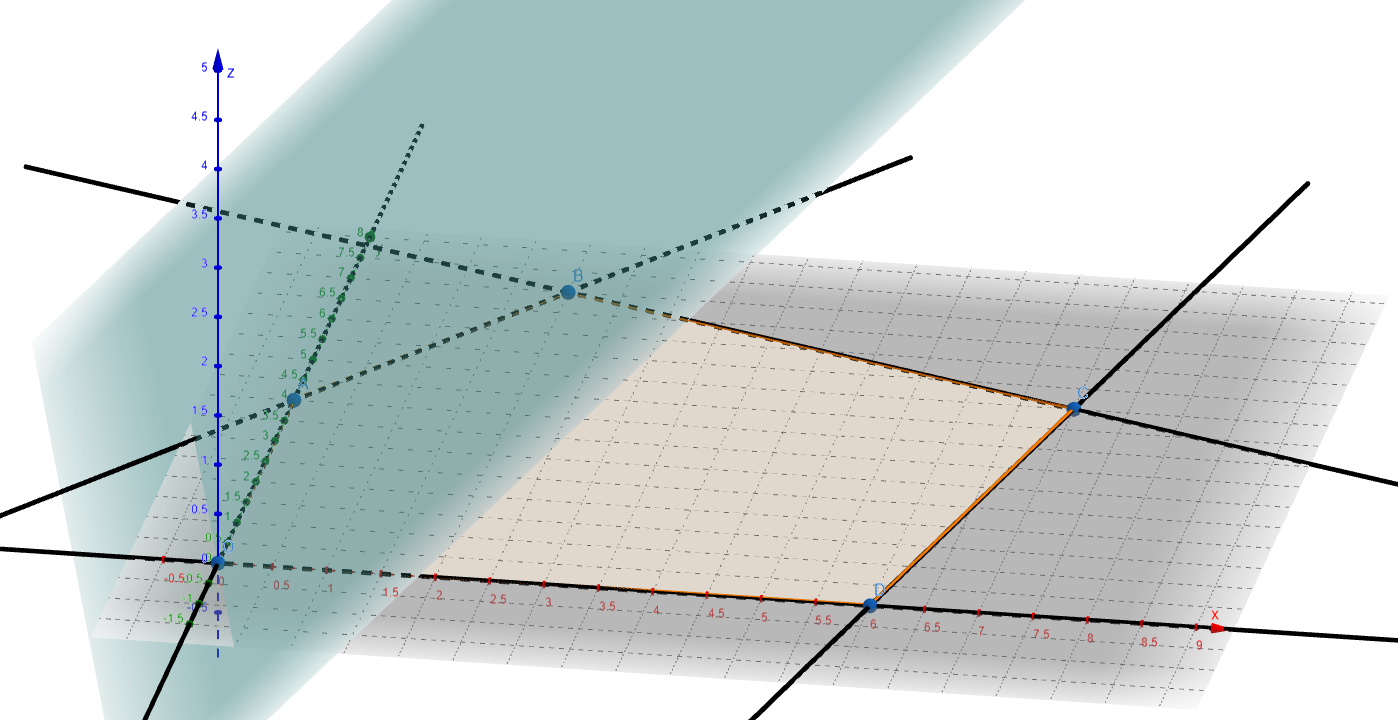
\includegraphics[width=0.45\linewidth]{example2.png}
    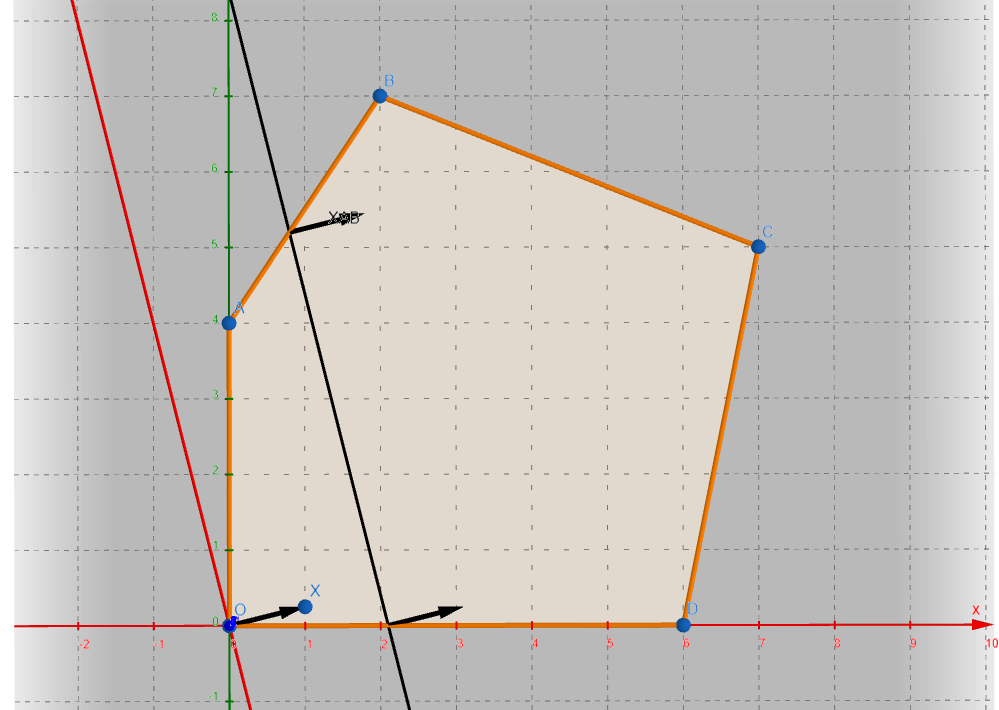
\includegraphics[width=0.45\linewidth]{Example3.png}
\end{figure}

ซึ่งถ้าใช้แนวคิดการไต่เขาตามให้ขนานกับแนวการไต่ระดับ จะพบว่าจุดสุดท้ายที่จะไต่ขึ้นไปได้คือจุด $C$ ด้วยการลากเส้นไต่ระดับขึ้นไปเรื่อย ๆ ดังรูป
\begin{figure}[h]
    \centering
    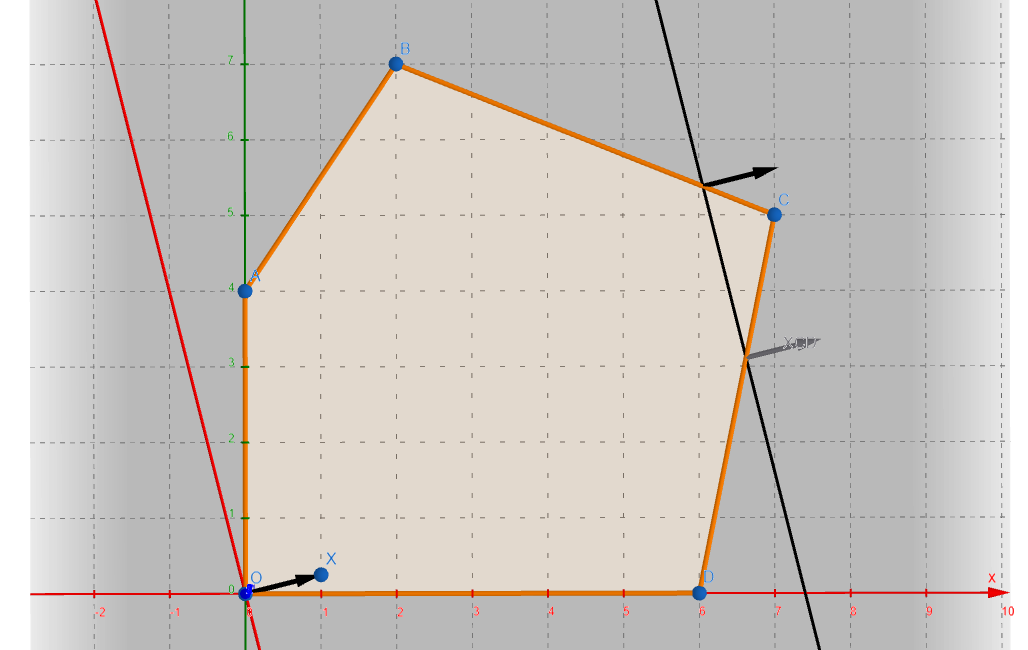
\includegraphics[width=0.75\linewidth]{Example4.png}
\end{figure}
และนอกจากวิธีการเลื่อนเส้นไต่ระดับแล้ว อีกวิธีที่ง่ายคือการลองแทนค่าทุกจุดยอดเพื่อคำนวณค่าจุดประสงค์แล้วเปรียบเทียบว่าค่าใดมากที่สุดหรือน้อยที่สุด

\begin{example}{โจทย์สำรวจคุณสมบัติ \ref{pro:linprogproperty}}{}
    พิจารณาโจทย์กำหนดการเชิงเส้น
    \begin{align*}
    \max  &\quad z=x+0.25y \\
    \text{subject to} &\quad x\geq0, \quad y\geq0\\
                &\quad y\leq1.5x+4\\
                &\quad y\leq-0.4x+7.8\\
                &\quad y\geq5x-30
    \end{align*}
    \begin{enumerate}
        \item จงแสดงว่าสมการเส้นตรงที่ระบุแนวหน้ากระดานการไต่ระดับ (เส้นที่เลื่อนตามรูปด้านบน) ที่ตัดแกน $y$ ที่ $y = c$ \underline{มีสมการเป็น $y=-4x + c$} กล่าวคือ แนวเส้นตรงที่มีความชัน $-4$ จะเป็นแนวที่ระนามมีค่าคงที่
        \item เมื่อพิจารณาบนแนวเส้นที่ทำให้ระนาบมีค่าคงที่ $y=-4x + 8$ เป็นตัวอย่าง จงหาจุดตัดของเส้นดังกล่าวกับเส้นตรง $y = 1.5x + 4$ กับเส้นตรง $y=0$
        \item จากจุดตัดที่ได้ในข้อที่ผ่านมา (ซึ่งมี 2 จุด) จงแสดงว่าทั้งสองจุดดังกล่าวให้ค่า $z=x + 0.25y$ \underline{เป็น $z = 2$}
        \item เมื่อพิจารณาบนแนวเส้นที่ทำให้ระนาบมีค่าคงที่ $y=-4x + c$ จงแสดงว่า \underline{ค่าคงที่ของระนาบคือ $z = 0.25c$}
    \end{enumerate}
\end{example}

\newpage
\begin{example}{แก้ปัญหากำหนดการเชิงเส้น 2 ตัวแปรด้วยการวาดภาพ}{}
    จงแก้โจทย์กำหนดการเชิงเส้นในตัวอย่าง \ref{ex:sampleLinProg} ด้วยวิธีวาดภาพ โดยพิจารณาค่าสูงสุดทั้งวิธีการไต่ระดับ และวิธีการลองแทนค่าทุกจุดยอด
\end{example}
\newpage
\begin{example}{แก้ปัญหากำหนดการเชิงเส้น 2 ตัวแปรด้วยการวาดภาพ}{}
    จงแก้โจทย์กำหนดการเชิงเส้นในตัวอย่าง \ref{ex:2varformulate} ด้วยวิธีวาดภาพ โดยพิจารณาค่าสูงสุดทั้งวิธีการไต่ระดับ และวิธีการลองแทนค่าทุกจุดยอด
\end{example}
\begin{solution}
    จากข้อที่ผ่านมา เราได้มาแล้วว่ากำหนดการเชิงเส้นคือ
    \begin{align*}
        \max  &\quad z=4000a + 1800b \\
        \text{s.t.} &\quad100a + 70b \leq 6000\\
                    &\quad800a + 600b \leq 100000\\
                    &\quad16a + 16b \leq 1000\\
                    &\quad a, b\geq0
        \end{align*}
    \begin{enumerate}[label=\textbf{ขั้นที่ \arabic*:}, align=left, labelwidth=5em, labelsep=1em, leftmargin=*, itemsep=16pt, topsep=0pt, parsep=0pt, partopsep=0pt]
    
    \item วาดรูปภาพเงื่อนไข โดยเรามี 3 เงื่อนไขดังนี้
        \begin{itemize}
            \item $100a + 70b = 6000$
            \item $800a + 600b = 100000$
            \item $16a + 16b = 1000$
        \end{itemize}
        ซึ่งทำได้โดยการหาจุดตัดแกน ซึ่งจะได้ดังนี้\\
        
        \begin{tabular}{|c|c|c|}
        \hline
            สมการ & จุดตัดแกน $x$ ($a$) & จุดตัดแกน $y$ ($b$) \\
            \hline
            $100a + 70b = 6000$ & 60 & 600/7 $\approx$ 85.71\\
            \hline
            $800a + 600b = 100000$ & 125 & $\approx$ 166.67\\
            \hline
            $16a + 16b = 1000$ & 62.5 & 62.5\\
            \hline
        \end{tabular}
        \begin{figure}[h]
            \centering
            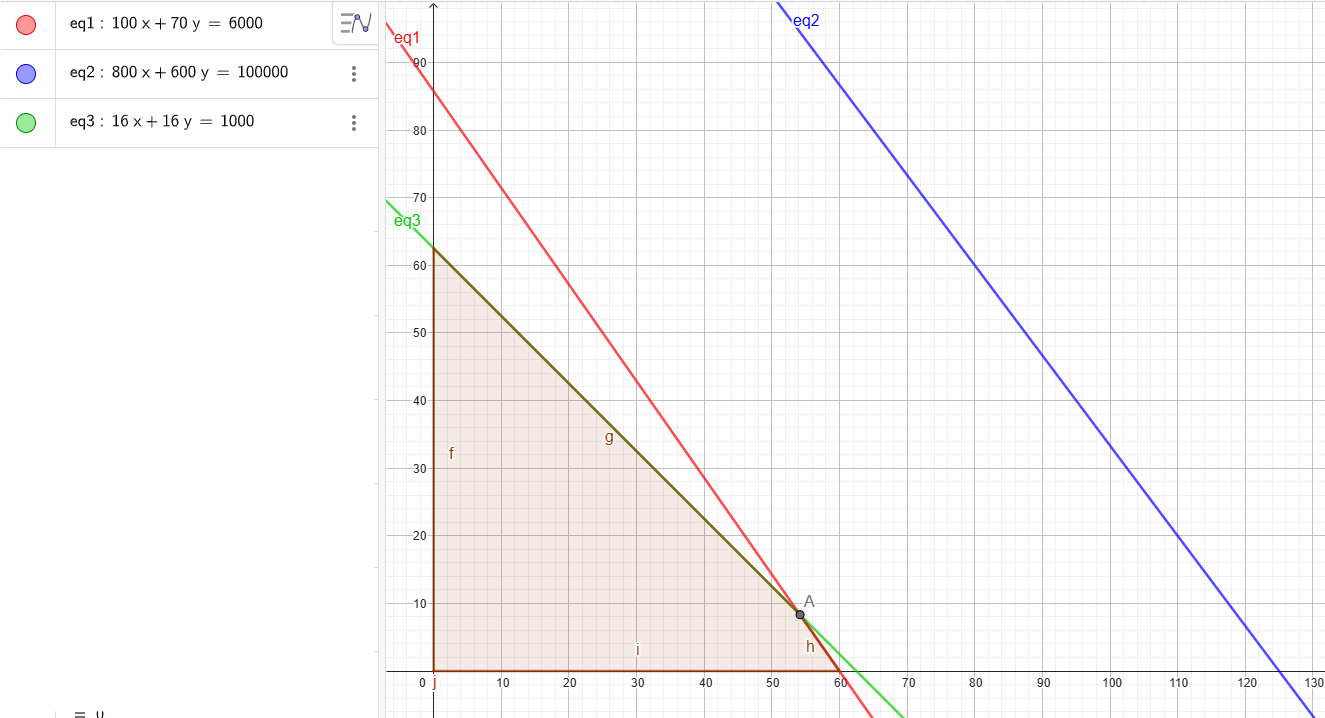
\includegraphics[width=0.75\linewidth]{ex113-1.png}
        \end{figure}
        และถ้าหาจุดตัดจากสมการที่ 1 และสมการที่ 3 ที่ตัดกันจะได้จุด $\approx(54.17,8.33)$

    \item แทนค่าจุดมุมลงในฟังก์ชันจุดประสงค์เพื่อหาค่าแล้วเปรียบเทียบกันว่าจุดใดให้ค่าจุดประสงค์มากที่สุด\\

    \begin{tabular}{c|c}
        $(a,b)$ & $\text{ยอดขาย} = 4000a + 1800b$ \\
        \hline
        $(0,62.5)\approx(0,62)$ & 111600 \\
        \hline
        $(54.17,8.33)\approx(54,8)$ & 230400 \\
        \hline
        $(60,0)$ & 240000 \\
        \hline
        $(0,0)$ & 0 \\
        \hline
    \end{tabular}

    \item สรุปคำตอบ จะได้ค่ายอดขายมากสุดเท่ากับ 240000 เกิดขึ้นที่จุด $(60,0)$ กล่าวคือผลิตกระบวนการที่ 1 เป็นจำนวน 60 เครื่อง และไม่ผลิตกระบวนการที่ 2 เลย
    \end{enumerate}
    \begin{remark}
        {โจทย์เพิ่ม}{}
        จะเห็นว่ากระบวนการที่ 2 ไม่ถูกใช้งานเลย ซึ่งอาจไม่เป็นที่พึงพอใจกับฝ่ายจัดซื้อที่ลงทุนไปกับการซื้อเครื่องมือสำหรับกระบวนการที่ 2 ไปแล้ว (เช่นกรณีกระบวนการที่ 2 เป็นเรื่องของเครื่องจักร) แต่เมื่อฝ่ายการตลาดทำการสำรวจเพิ่มเติม พบว่าเรายังสามารถทำสินค้า Y ให้มีภาพลักษณ์ที่พรีเมียมมากขึ้นเพื่อเปลี่ยนกลุ่มลูกค้าไปกลุ่มที่กำลังจ่ายสูงขึ้นได้ (เนื่องจากผลิตได้น้อยเมื่อเทียบกับ X ที่ผลิตได้ 4 ชิ้นต่อครั้งของกระบวนการที่ 1) ดังนั้นฝ่ายการตลาดจึงมาถามเราที่เป็นที่ปรึกษาทางธุรกิจว่าควรตั้งราคาขายสินค้า Y ให้อยู่ในช่วงราคาเท่าไหร่เพื่อให้ผลเฉลยที่ให้ยอดขายสูงสุดมาจากการใช้ทั้งเครื่องจักรของกระบวนการที่ 1 และเครื่องจักรของกระบวนการที่ 2\\

        นอกจากการปรับราคาแล้ว ยังมีทางเลือกอื่นใดบ้างในการปรับปรุงแบบจำลองให้ยังคงใช้ทั้ง 2 กระบวนการ โดยที่ไม่ต้องปรับราคา (แต่อาจจะได้ยอดขายรวมน้อยลงบ้างก็ยังยอมรับได้)
    \end{remark}
\end{solution}

\section{แนวคิดเบื้องต้นของวิธีซิมเพล็กซ์ (Simplex)}
ในหัวข้อที่แล้ว เราศึกษาวิธีการแก้ปัญหากำหนดการเชิงเส้นด้วยวิธีการรูปภาพ ซึ่งข้อจำกัดของวิธีการดังกล่าวคือเราจะสามารถแก้ปัญหาได้แค่กรณี 2 ตัวแปร และจริง ๆ แล้ว เราสามารถทำกับปัญหา 3 ตัวแปรก็ได้เช่นกันแต่จะวาดภาพยากกว่า เพราะต้องดูขอบเขตผลเฉลยใน 3 มิติ แต่ว่าถ้า 4 ตัวแปรเป็นต้นไปเราจะไม่สามารถวาดภาพได้อีกแล้ว ทำให้วิธีการดังกล่าวใช้ไม่ได้อีกต่อไป

\begin{figure}[h]
    \centering
    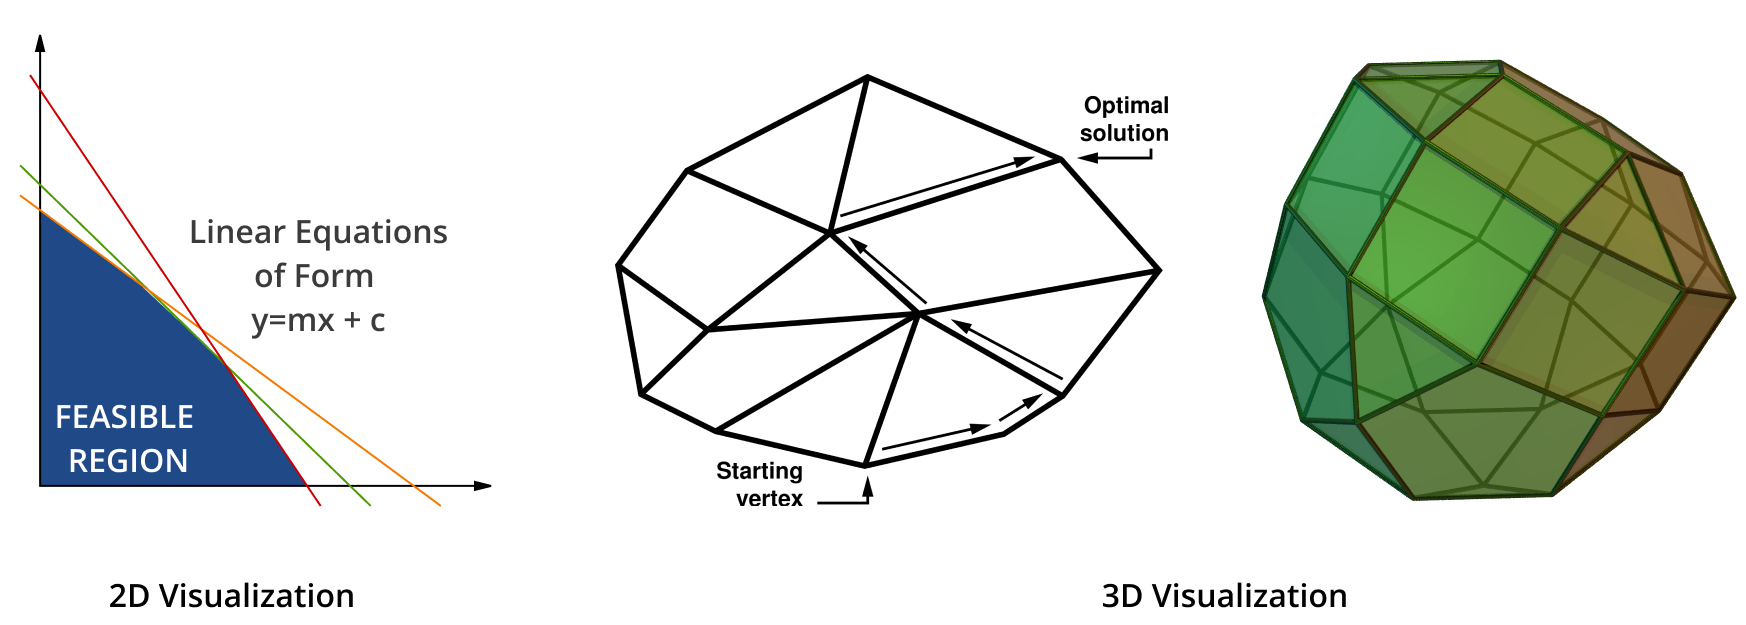
\includegraphics[width=1\linewidth]{simplex1.png}
\end{figure}

เครื่องมือที่จะใช้ในการแก้ปัญหากำหนดการเชิงเส้นสำหรับกรณีใด ๆ ก็ตามที่จะศึกษาในหัวข้อนี้คือวิธีซิมเพล็กซ์ (simplex method) ซึ่งเป็นกระบวนการในการใช้การดำเนินการทางเมทริกซ์เพื่อการเปลี่ยน pivot ที่จะให้ค่าสูงขึ้นเรื่อย ๆ ไล่ไปตามขอบของรูป โดยอาศัยคุณสมบัติตามที่เราได้ศึกษามาในกรณี 2 มิติว่าการเดินตามขอบบนบริเวณที่เป็นรูปนูน (convex) จะพาเราไปจุดผลเฉลยค่าสุดขีดได้แน่ ๆ

\begin{figure}[h]
    \centering
    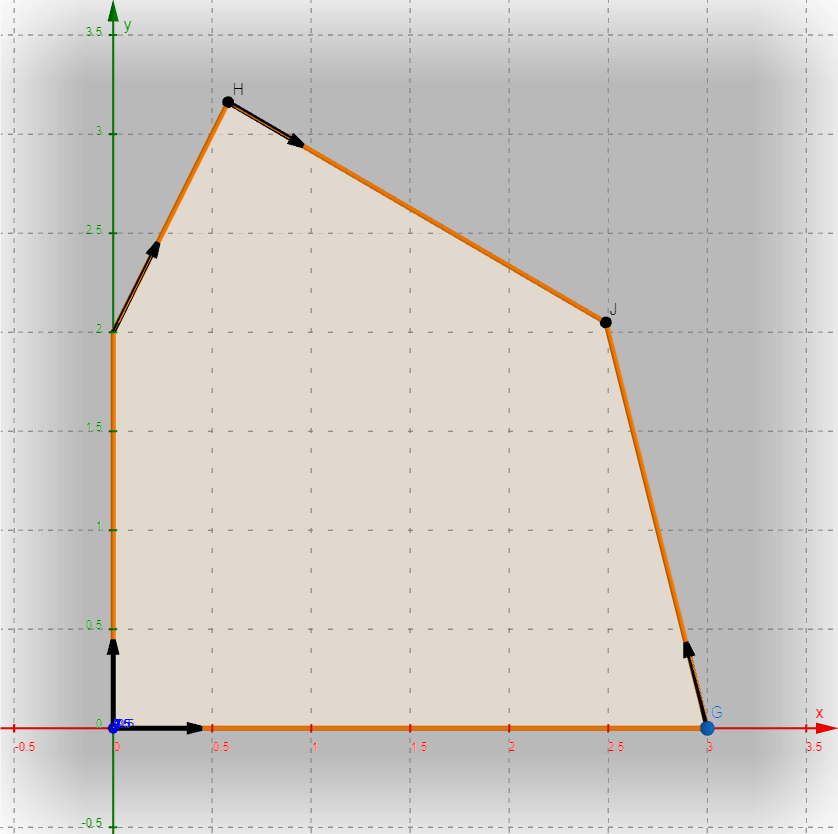
\includegraphics[width=0.5\linewidth]{simplex2.png}
\end{figure}

ทั้งนี้ สิ่งหนึ่งที่ต้องเน้นย้ำสำหรับขั้นตอนกระบวนการนี้คือสมมติฐานการเป็นรูปนูน เพราะอัลกอริทึมที่กำลังจะได้ศึกษาอาศัยการเดินตามเส้นขอบตามทิศทางที่มีค่าเพิ่มได้ ซึ่งเงื่อนไขที่การันตีการไปจุดผลเฉลยสุดขีดได้คือการเป็นรูปนูนที่ทำให้เราไต่ระนาบขึ้นได้เรื่อย ๆ เสมอตามรูปด้านบนที่เราสามารถเดินทางจากจุด $O$ ไปที่จุด $J$ ที่เป็นผลเฉลยได้ แต่ถ้ารูปพื้นที่เป็นไปได้ไม่ใช่รูปนูน อาจทำให้เกิดปัญหาที่เรียกว่าการติดค่าสุดขีดสัมพัทธ์ (local extrema) ตามรูปด้านล่าง ซึ่งถ้าเริ่มที่จุด $O$ จะเดินไปได้ไกลสุดแค่จุด $H$ หรือจุด $G$ เท่านั้นตามแนวคิดเบื้องต้นของ simplex แต่ในวิชานี้ เราจะโฟกัสไปแค่ที่โจทย์ที่พื้นที่ผลเฉลยเป็นรูปนูนอยู่แล้ว ดังนั้นนักศึกษาจึงไม่ต้องกังเรื่องสมมติฐานดังกล่าว

\begin{figure}[h]
    \centering
    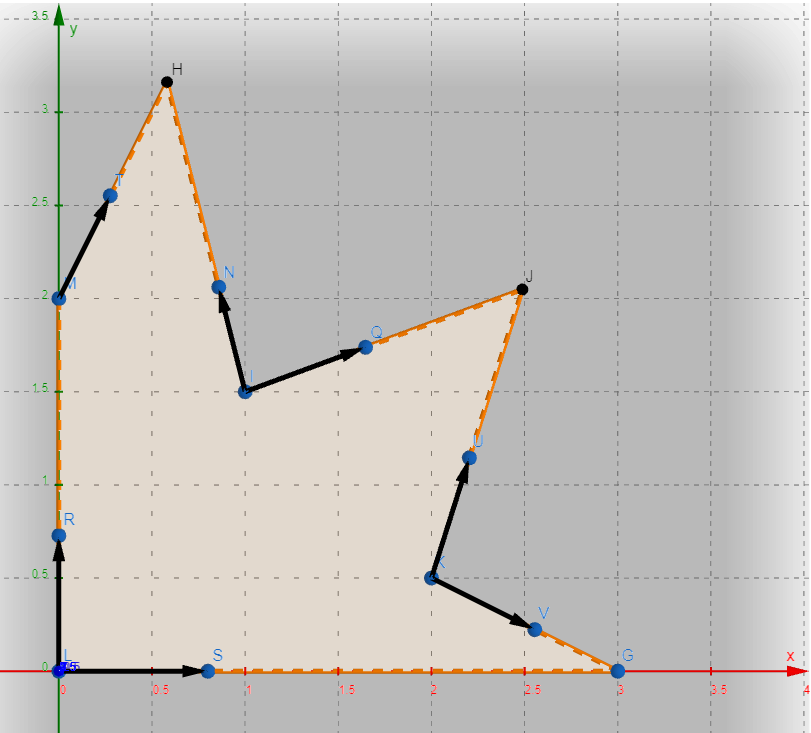
\includegraphics[width=0.4\linewidth]{simplex3.png}
\end{figure}

\subsubsection*{แนวคิดเชิงการคำนวณ (อ่านนอกเวลาเพิ่มเติม): wait revise again}
จะขอเริ่มจากตัวอย่างที่ง่ายเพื่อพาไปดูหลักการคิดทีละขั้น (สำหรับนักศึกษาที่สนใจ simplex method เลยสามารถข้ามหัวข้อนี้ได้) โดยปัญหากำหนดการเชิงเส้นที่จะพิจารณาคือ
\begin{align*}
    \max  &\quad 4x + y \\
    \text{subject to} &\quad x\geq0, \quad y\geq0\\
                &\quad x\leq 4\\
                &\quad y\leq 4
\end{align*}
และมีบริเวณการพิจารณาตามรูปด้านล่างนี้ ในรูปจะมีเวกเตอร์แนวการไต่ระดับของระนาบอยู่ และจะเห็นว่าจุด $(4,4)$ ควรเป็นจุดที่ให้ค่าสูงสุดแน่นอน
\begin{figure}[h]
    \centering
    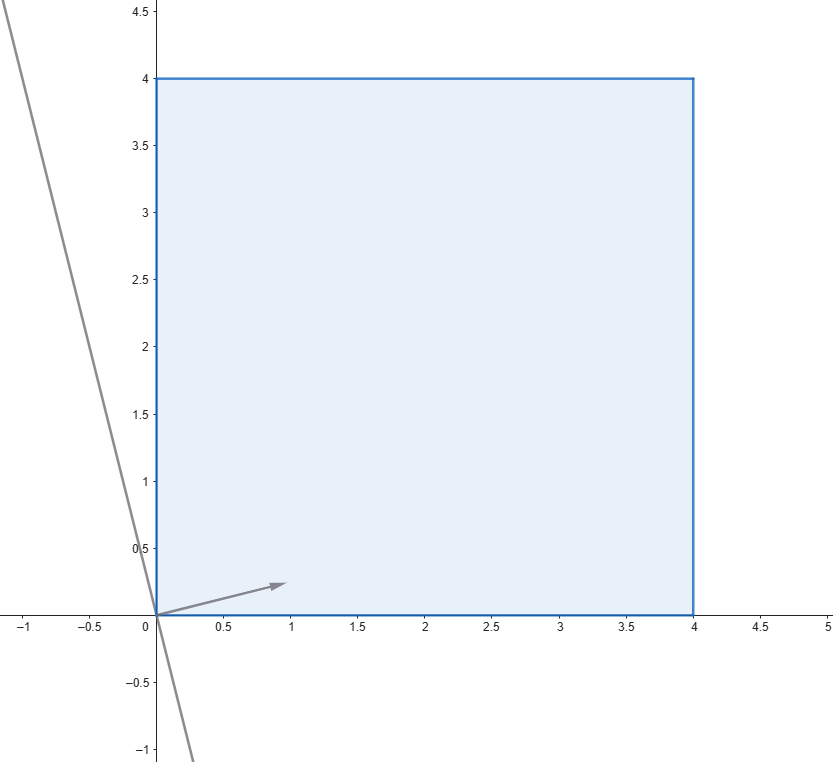
\includegraphics[width=0.4\linewidth]{basicSimplex1.png}
\end{figure}

แต่รูปแบบอสมการนั้นเป็นรูปแบบที่ไม่เหมาะกับการแก้ปัญหาในเชิงการคำนวณ ทำให้เราต้องเปลี่ยนรูปแบบการเขียนให้อยู่ในรูปแบบสมการเท่ากับ ซึ่งอาศัยคุณสมบัติของระบบจำนวนว่า
\begin{property}
    {เปลี่ยนอสมการเป็นสมการ}{}
    $$
    x \leq a \text{ ก็ต่อเมื่อ มีจำนวนจริง } s \text{ ที่เป็นบวกหรือศูนย์ที่ทำให้ } x+s = a
    $$
    ซึ่งตัวแปร $s$ ในที่นี้มีชื่อเรียกว่าตัวแปรส่วนเกิน (slack variable)
\end{property}

ซึ่งแน่นอนว่าตัวแปรส่วนเกินนี้จะเป็นเพียงแค่ตัวแปรที่เพิ่มเข้ามาในเงื่อนไข ไม่มีผลต่อค่าของฟังก์ชันจุดประสงค์ ดังนั้น เหล่าบรรดาเงื่อนไขอสมการจะต้องมีการเติมตัวแปรส่วนเกินเพื่อทำให้เป็นเงื่อนไขสมการได้ดังนี้
\begin{align*}
    \max  &\quad 4x + y + 0s_1 + 0s_2 \\
    \text{subject to} &\quad x, y, s_1, s_2\geq0\\
                &\quad x + s_1 = 4\\
                &\quad y + s_2 = 4
\end{align*}
หมายเหตุสำคัญตัวแปรทุกตัวจะต้องไม่ต่ำกว่า 0 เป็นเงื่อนไขบังคับ

ทีนี้ จะขอกล่าวถึงความหมายของตัวแปรส่วนเกินเชิงรูปภาพกันก่อนว่าคืออะไรในรูปภาพ ทั้งนี้อย่าลืมว่า simplex method คือการเดินตามขอบจากจุดยอดหนึ่งไปยังอีกจุดยอดหนึ่ง เพราะฉะนั้น เราจะพิจารณาแค่จุดตามขอบเท่านั้น รูปภาพด้านล่างนี้เป็นตัวอย่างค่าตัวแปรของจุดตามตำแหน่งขอบต่าง ๆ ซึ่งจะเห็นว่าตัวแปร $s_1$ ทีเป็นตัวแปรส่วนเกินของตัวแปร $x$ คือตัวแปรที่จะเติมเต็มให้ $x$ เดินไปถึงจุดยอดได้ และถ้าพิจารณาตามจุดยอดต่าง ๆ ก็จะพบว่าระหว่างตัวแปรของปัญหาและตัวแปรส่วนเกินที่คู่กันนั้นจะต้องมีอย่างน้อย 1 ตัวที่แปรที่มีค่าเป็น 0 ตัวอย่างเช่นการเดินตามขอบด้านล่างของรูปภาพในตัวอย่างนี้คือการแลกค่ากันระหว่าง $x$ และ $s_1$ โดยสมการ $x + s_1 = 4$ ที่จุดยอดซ้ายคือจุดที่ $x=0, s_1=4$ ในขณะที่จุดด้านขวาคือจุดที่ $x=4,s_1=0$ กล่าวคือ การเดินตามขอบของบริเวณที่เป็นไปได้จากจุดยอดไปอีกจุดยอดก็คือการพยายามแลกเปลี่ยนค่าของตัวแปรส่วนเกินให้เป็น 0 นั่นเอง

\begin{figure}[h!]
    \centering
    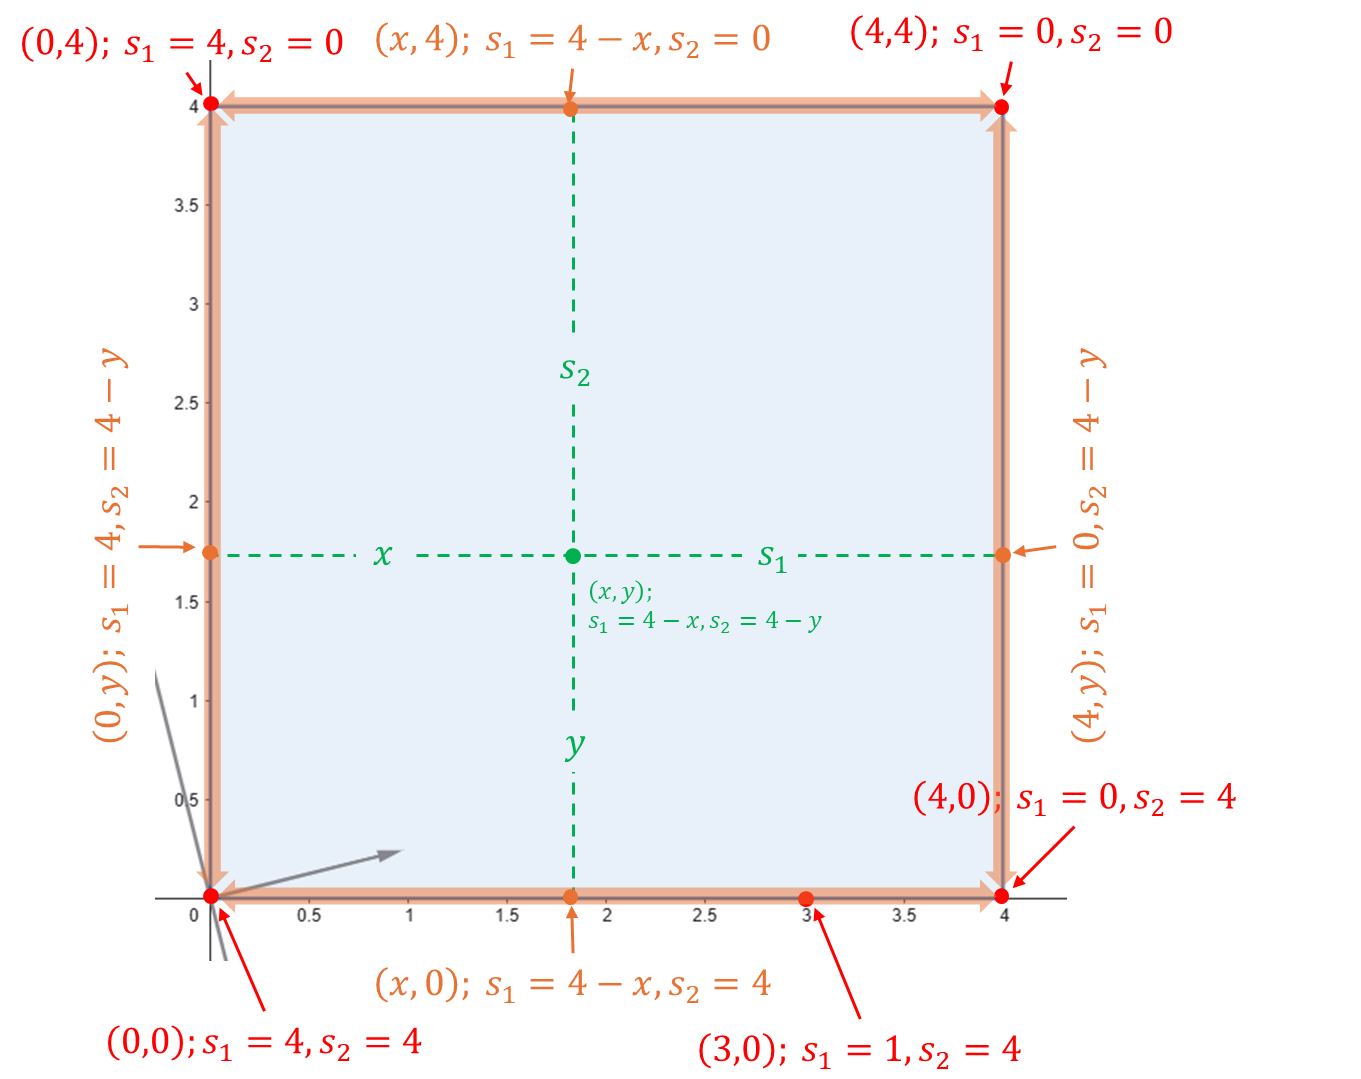
\includegraphics[width=0.7\linewidth]{basicSimplex2.png}
    \caption{Enter Caption}
    \label{fig:enter-label}
\end{figure}

จากที่กล่าวไปสักครู่ คือวิธีการเดินทางกรณีที่รู้แล้วว่าจะเดินตามขอบใด
คำถามต่อมาคือ เมื่อเรายืนอยู่ที่จุดยอดหนึ่ง จะรู้ได้อย่างไรว่าต้องเดินไปทางไหน ตัวอย่างเช่นถ้าเรากำลังยืนอยู่ที่จุด $(0,0)$ จะรู้ได้อย่างไรว่าต้องเดินตามขอบแนวตั้งไปที่ $(0,4)$ หรือตามขอบแนวนอนไปที่ $(4,0)$
ซึ่งถ้าอาศัยความรู้ในวิชาแคลคูลัสในแง่ขอการดูอัตราการเปลี่ยนแปลง จะทราบได้ทันทีว่าต้องเดินตามแนวแกน $x$ เพราะแนวการเดินใกล้กับเวกเตอร์ระบุทิศทางของระนาบมากที่สุด ซึ่งจริง ๆ แล้วก็สามารถดูได้โดยง่ายจากสัมประสิทธิ์ของตัวแปรในสมการ $z=4x+y+0s_1+0s_2$ ที่หมายความว่าการเดินตาม $x$ จะเปลี่ยนค่า $z$ เป็นระยะ 4 หน่วยเมื่อเพิ่ม $x$ ไป 1 หน่วย ในขณะที่ถ้าเดินตาม $y$ จะเปลี่ยนค่าแค่ 1 หน่วยเท่านั้น

ดังนั้น เราจึงสามารถตัดสินใจได้ว่าเราจะเดินตาม $x$ โดยจากเดิมที่ตรึง $x=0, y=0$ เราจะเปลี่ยนไปตรึง $s_1=0, y=0$ ซึ่งลักษณะการพิจารณาชุดตัวแปรในลักษณะนี้เราจะเรียกว่าชุดตัวแปรพื้นฐาน (basic variables) ซึ่งคือชุดตัวแปรที่จะถูกมองให้มีค่าเป็น 0 เพื่อใช้คำนวณค่าตัวแปรที่ไม่ใช่ตัวแปรพื้นฐาน (non-basic variables) กล่าวคือ จากเดิมที่เรากำหนดระบบเป็น $s_1 = 4 - x$ และ $s_2 = 4 - y$ โดยที่ $x=0, y=0$ จะโดนเปลี่ยนการพิจารณาระบบเป็น $x = 4 - s_1$ และ $s_2 = 4 - y$ โดยที่ $s_1=0, y=0$ ซึ่งเรียกการดำเนินการนี้ว่าการหมุนตัวแปรหลัก (pivot change) จากเดิมที่ $s_1, s_2$ เป็นตัวแปรหลัก (pivot variable) เราจะเปลี่ยนระบบให้ $x, s_2$ เป็นตัวแปรหลักแทน

สำหรับการดำเนินการหมุนตัวแปรหลัก ตัวแปรหลักจะไม่สามารถมีเพิ่มได้ ในตัวอย่างจะมีได้แค่ 2 ตัวแปร ดังนั้น การจะนำตัวแปรใหม่เข้ามาเป็นตัวแปรหลัก จึงต้องมีการนำ pivot ตัวเก่าออกหนึ่งตัว ซึ่งจะตามมาด้วยคำถามว่ารู้ได้อย่างไรว่าต้องเอา $s_1$ ออกจากการเป็นตัวแปรหลักแล้วนำ $x$ มาแทนที่
ซึ่งแนวคิดที่ใช้ในการเดินทางจริง ๆ เป็นเรื่องการเดินตามแนวตัวแปรหลักใหม่อย่างไรให้ไม่หลุดออกจากขอบ ซึ่งเห็นได้ชัดว่าถ้าเดินให้สั้นที่สุดเท่าที่จำเป็นเพื่อจะไปเจอขอบหนึ่งจะการันตีได้ว่าเราจะไม่เดินหลุดขอบแน่นอน ซึ่งคุณสมบัติของการเป็นรูปนูนคือจะไม่มีเส้นขอบใดที่ลากต่อแล้วตัดภายในพื้นที่เสมอดังรูปด้านล่างนี้
เพราะฉะนั้น ในทางปฏิบัติที่เราอาจไม่เห็นรูปภาพ เราจึงต้องเลือกการเดินที่สั้นที่สุดเอาไว้ก่อนเพื่อให้ไม่หลุดขอบถึงแม้จะไม่ใช่ทางที่เร็วที่สุดก็ตาม
และเมื่อทราบแล้วว่าต้องเดินไปชนขอบใด จึงค่อยพิจารณาว่าขอบนั้นเป็นขอบประชิดของตัวแปรส่วนเกินตัวไหน

\begin{figure}
    \centering
    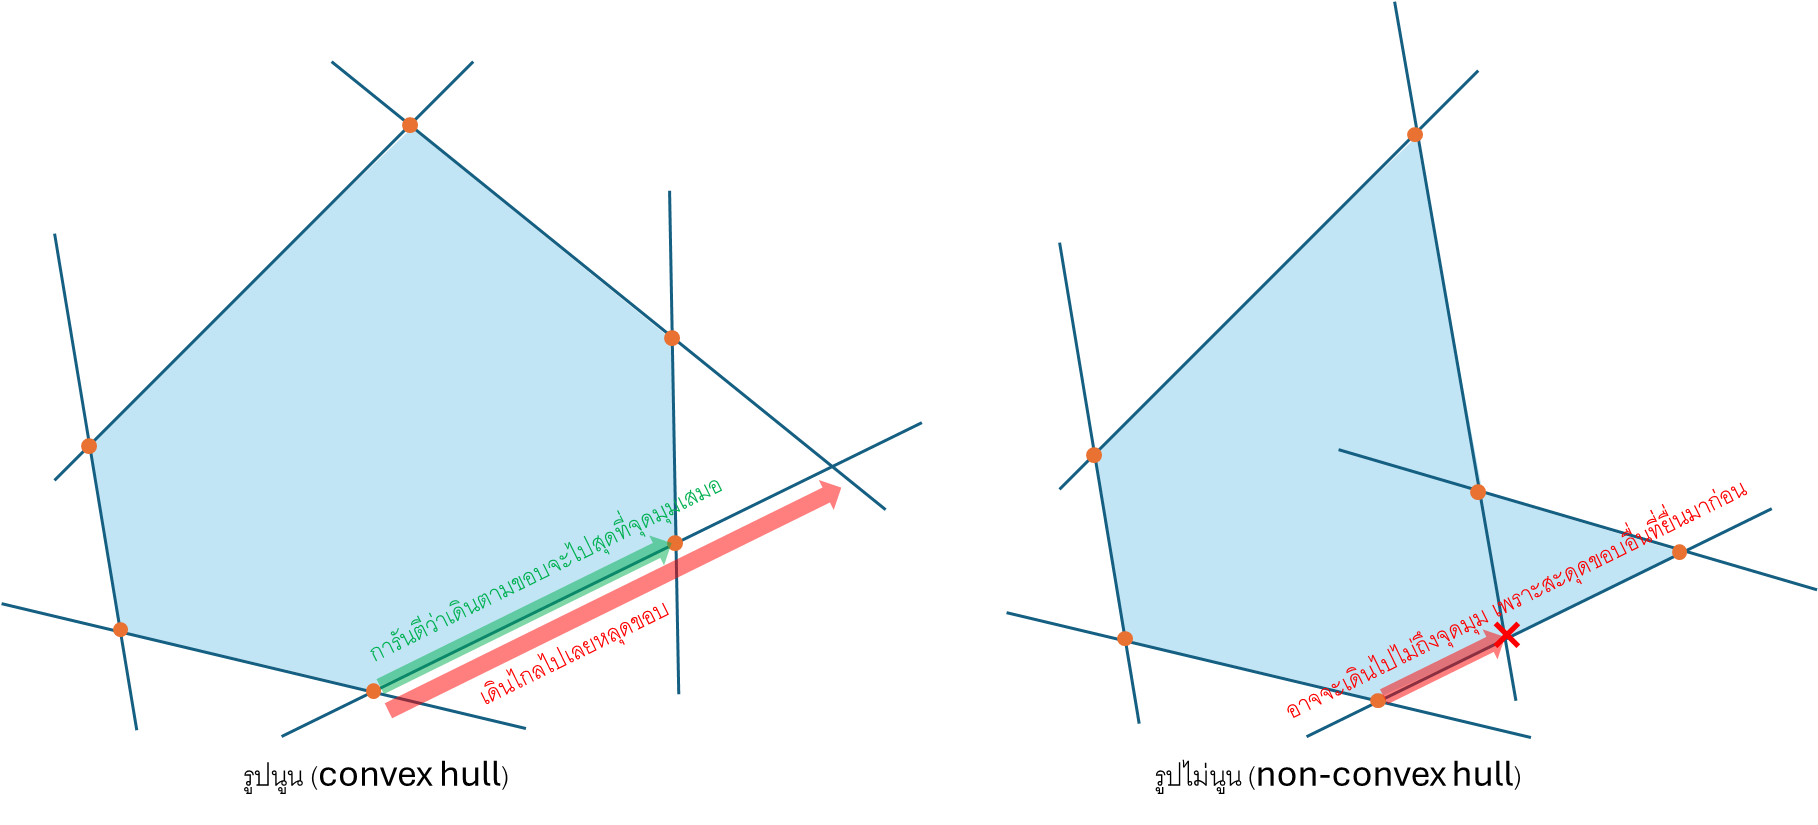
\includegraphics[width=0.8\linewidth]{SimplexConvexHull.png}
    \caption{Enter Caption}
    \label{fig:enter-label}
\end{figure}

จากตัวอย่างที่เรากำลังพิจารณาอยู่นั้น เราทราบแล้วว่าเราต้องเดินจาก $(0,0)$ ตามแนวตัวแปร $x$ แต่เนื่องจากรูปนี้ยังเป็นรูปอย่างง่ายจึงเห็นชัดว่ามีเส้นทางเดียวเท่านั้นที่ไปได้เมื่อบังคับให้เปลี่ยน $x$ คือเดินตามขอบแนวด้านล่าง และจะไปประชิดที่ขอบ $x=4$ ซึ่งคือขอบที่ตัวแปรส่วนเกิน $s_1=0$ จึงทำให้ทราบว่าเราต้องนำ $x$ ไปเป็นตัวแปรหลักแทน $s_1$ และให้ $s_1$ ทำหน้าที่ตัวแปรพื้นฐาน กล่าวคือ ตั้งให้ $s_1=0$ และ $y=0$ เป็นตัวแปรพื้นฐานและได้ว่า $x=4, y=0$ เพราะฉะนั้น จาก $z=4\times 0 + 1\times0 + 0\times 4 + 0\times 4 = 0$ ที่จุด $(0,0)$ จะได้ว่าค่าจุดประสงค์ ณ ปัจจุบันเปลี่ยนไปเป็น $z=4\times 4 + 1\times0 + 0\times 0 + 0\times 4 = 16$ และเราจะไม่เดินตาม $x$ อีกแล้ว

กล่าวคือตอนนี้ระบบเหลือแค่ปัญหา
\begin{align*}
    \max  &\quad y + 0s_2 + 16 \\
    \text{subject to} &\quad y, s_2\geq0\\
                &\quad y + s_2 = 4
\end{align*}
ซึ่งจะเห็นว่าเปรียบเสมือนการเดินตามแนว $y$ โดยที่จะเอา $y$ ไปเป็นตัวแปรหลักแทน $s_2$ จึงไปจบที่ขอบที่ $s_2=0$ ทำให้ได้ $y=4$ และจบด้วยการไม่สามารถปรับค่าตัวแปรไหนเพิ่มเติมได้อีกแล้ว จึงได้ว่า $(x,y) = (4,4)$ เป็นผลเฉลยที่ทำให้ได้ฟังก์ชันค่าจุดประสงค์มากที่สุด และเท่ากับ $z = 4\times 4 + 1\times 4 = 20$

ทั้งนี้ ขอสรุปขั้นตอนสำคัญของการทำ simplex method ดังนี้
\begin{enumerate}
    \item หา pivot ตัวใหม่: พิจารณาหาทิศทางที่ทำให้เปลี่ยนค่าได้เร็วสุดก่อน
    \item หา pivot ตัวที่จะถูกแทนที่: เมื่อทราบแนวการเปลี่ยนแล้ว ให้ดูว่าจุดที่ยืนอยู่ปัจจุบันมีเส้นทางไหนที่เดินแล้วถึงขอบเร็วสุดเพื่อป้องกันการหลุดนอกขอบ แล้วตัวแปรส่วนเกินของขอบนั้นจะโดนแทนที่กลายไปเป็นตัวแปรพื้นฐาน (ตัวแปรที่ถูกตั้งค่าให้เป็น 0)
    \item กำจัดตัวแปร pivot ใหม่ออกจากระบบ
    \item ทำวนไปเรื่อย ๆ จนไม่สามารถเปลี่ยนตัวแปรใด ๆ เพื่อเพิ่มค่าจุดประสงค์ได้อีกแล้ว
\end{enumerate}

\subsection{Simplex Method Algorithm}
ในการทำ simplex นั้นจะนิยมเขียนการคำนวณอยู่ในรูปแบบเมทริกซ์ที่เรียกว่า simplex tableau ดังนี้
\begin{center}
\renewcommand{\arraystretch}{1.4}
\begin{tabular}{|c|cccccc|c|}
\hline
\textbf{Pivot} & $x_1$ & $x_2$ & $\cdots$ & $x_n$ & $s_1$ & $\cdots$ & \textbf{RHS} \\
\hline
$x_{B_1}$ & $c_{11}$ & $c_{12}$ & $\cdots$ & $c_{1n}$ & $c_{1s_1}$ & $\cdots$ & $b_1$ \\
$x_{B_2}$ & $c_{21}$ & $c_{22}$ & $\cdots$ & $c_{2n}$ & $c_{2s_1}$ & $\cdots$ & $b_2$ \\
$\vdots$ & $\vdots$ & $\vdots$ & & $\vdots$ & $\vdots$ & & $\vdots$ \\
$x_{B_m}$ & $c_{m1}$ & $c_{m2}$ & $\cdots$ & $c_{mn}$ & $c_{ms_1}$ & $\cdots$ & $b_m$ \\
\hline
$Z$ & $z_1$ & $z_2$ & $\cdots$ & $z_n$ & $z_{s_1}$ & $\cdots$ & $z$ \\
\hline
\end{tabular}
\end{center}
โดยจะกล่าวละเอียดทีละขั้น โดยมีขั้นตอนดังนี้

\begin{algorithm}
    {Simplex Method}{}
    ก่อนอื่น ตัวแปรทุกตัวต้องไม่ติดลบ ($x_i \geq 0$) และเงื่อนไขอยู่ในรูปแบบซึ่งก้อนตัวแปรอยู่ฝั่งซ้ายและค่าคงที่อยู่ฝั่งขวาโดยที่ค่าคงที่ต้องไม่ติดลบ
    \begin{enumerate}[label=\textbf{ขั้นที่ \arabic*.}, align=left, labelwidth=5em, labelsep=1em, leftmargin=*, itemsep=0pt, topsep=0pt, parsep=0pt, partopsep=0pt]
 
  \item \textbf{แปลงปัญหาให้อยู่ในรูปแบบมาตรฐาน (Standard Form)}  
  \begin{itemize}[itemsep=0pt, topsep=0pt, parsep=0pt, partopsep=0pt]
    \item เป้าหมายต้องอยู่ในรูปแบบ \textbf{Maximize $Z = c_1x_1 + c_2x_2 + \dots + c_nx_n$}
    \item ข้อจำกัดต้องอยู่ในรูป \textbf{สมการ} โดยการเพิ่มตัวแปรประเภท \textit{slack, surplus, artificial} ตามความเหมาะสม
  \end{itemize}

  \item \textbf{เขียน Simplex Tableau แรก}  
  \begin{itemize}[itemsep=0pt, topsep=0pt, parsep=0pt, partopsep=0pt]
    \item สร้างตารางแสดงสัมประสิทธิ์ของตัวแปรในแต่ละ constraint
    \item เพิ่มแถวของสมการ $Z$ และค่าคงที่ (RHS)
  \end{itemize}

  \item \textbf{เลือกตัวแปรที่จะเข้าสู่ฐาน (Entering Variable)}  
  \begin{itemize}[itemsep=0pt, topsep=0pt, parsep=0pt, partopsep=0pt]
    \item เลือกตัวแปรที่มีสัมประสิทธิ์ในแถว $Z$ น้อยที่สุด (ติดลบมากที่สุด)
    \item ถ้าไม่มีค่าสัมประสิทธิ์ใดติดลบในแถว $Z$: หยุดได้เลยเพราะได้คำตอบที่เหมาะสมแล้ว
  \end{itemize}

  \item \textbf{ทำ Minimum Ratio Test เพื่อเลือกตัวแปรที่จะออกจากฐาน (Leaving Variable)}  
  \begin{itemize}[itemsep=0pt, topsep=0pt, parsep=0pt, partopsep=0pt]
    \item สำหรับแต่ละแถวที่ตัวแปรเข้ามามีสัมประสิทธิ์เป็นบวก ให้คำนวณ:
    \[
    \text{Ratio} = \frac{\text{RHS}}{\text{ค่าสัมประสิทธิ์ของตัวแปรเข้าใหม่}}
    \]
    \item เลือกแถวที่ให้ค่า Ratio ต่ำสุด
    \item ถ้าไม่มี Ratio ใดสามารถคำนวณได้ (ทุกสัมประสิทธิ์ ≤ 0) → ปัญหา \textbf{ไม่จำกัดคำตอบ} (Unbounded)
  \end{itemize}

  \item \textbf{ทำ Pivot เพื่ออัปเดต Tableau}  
  \begin{itemize}[itemsep=0pt, topsep=0pt, parsep=0pt, partopsep=0pt]
    \item ทำให้ตำแหน่ง Pivot (จุดตัดระหว่างแถวเข้าและออก) มีค่าเป็น 1
    \item ปรับแถวอื่นให้ค่าของตัวแปรเข้ามาในคอลัมน์นั้นเป็น 0
  \end{itemize}

  \item \textbf{ทำซ้ำขั้นตอนที่ 3–5 จนกว่าจะไม่มีสัมประสิทธิ์ติดลบในแถว $Z$}

  \item \textbf{อ่านคำตอบจาก Tableau สุดท้าย}  
  \begin{itemize}[itemsep=0pt, topsep=0pt, parsep=0pt, partopsep=0pt]
    \item ตัวแปรในฐานจะมีค่าตรงกับ RHS
    \item ตัวแปรที่ไม่อยู่ในฐานจะมีค่าเป็น 0
    \item ค่า $Z$ ที่เหมาะสมที่สุดอยู่ในมุมขวาล่างของแถว $Z$
  \end{itemize}

\end{enumerate}
\end{algorithm}

\subsubsection{กรณีที่ 1: เงื่อนไขมีแต่ $\leq$ (จุดกำเนิดเป็น basic feasible solution)}
กรณีนี้เป็นกรณีที่ง่ายที่สุด เพราะเป็นกรณีที่เริ่มกระบวน simplex ได้ทันทีที่จุดกำเนิดโดยไม่ต้องมีการปรับแต่งอะไรก่อนหน้า
ในการอธิบายวิธีการของกรณีนี้ จะขอใช้ตัวอย่างดังนี้
\begin{align*}
    \max \quad & 3x + 5y \\
    \text{subject to} \quad
    & x \geq 0, \quad y \geq 0 \\
    & x \leq 4 \\
    & y \leq 6 \\
    & 3x + 2y \leq 18
\end{align*}

\subsubsection*{ขั้นที่ 1: แปลงปัญหาให้อยู่ในรูปแบบมาตรฐาน (Standard Form)}
\begin{itemize}
  \item เป้าหมาย $\max 3x + 5y$ อยู่ในรูป \textbf{การเพิ่มค่า (Maximization)} อยู่แล้ว
  \item แต่ถ้าเป้าหมายเป็น \textbf{Minimization}, ต้องแปลงเป็น \textbf{Maximization} โดยเปลี่ยนเครื่องหมาย:
  \[
  \text{Minimize } Z = c_1x_1 + c_2x_2 \quad \Rightarrow \quad \text{Maximize } -Z = -c_1x_1 - c_2x_2
  \]
    \item ทุกตัวแปรต้องมีเงื่อนไข \textbf{ไม่ติดลบ}:
  \[
  x_i, s_i, a_i \geq 0
  \]
    ถ้าติดลบ ให้เปลี่ยนเป็นตัวแปรใหม่ $x_{new} = -x$ (แต่ในกรณีนี้ยังไม่มี)
  \item ข้อจำกัดทั้งหมดต้องเขียนในรูปสมการ (equalities) โดยข้อจำกัดแบบ $\leq$, ให้เพิ่ม \textbf{ตัวแปรส่วนเกิน (Slack Variable)} $s_i$: $a_1x_1 + a_2x_2 \leq b \quad \Rightarrow \quad a_1x_1 + a_2x_2 + s_i = b$

\end{itemize}
\begin{example}{เปลี่ยนรูปมาตรฐานกรณี 1}{}
    จงเปลี่ยนปัญหา
    \begin{align*}
        \max \quad & 3x + 5y \\
        \text{subject to} \quad
        & x \geq 0, \quad y \geq 0 \\
        & x \leq 4 \\
        & y \leq 6 \\
        & 3x + 2y \leq 18
    \end{align*}
    ให้อยู่ในรูปมาตรฐาน
\end{example}

\begin{center}
    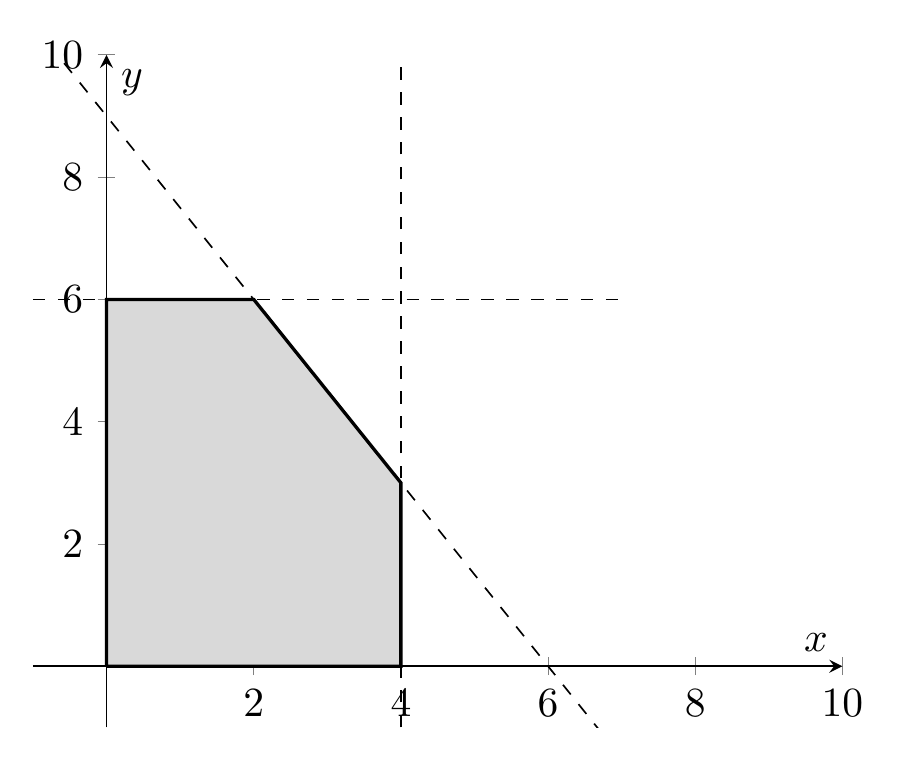
\begin{tikzpicture}[scale=1.5]
\begin{axis}[
  axis lines=middle,
  xmin=-1, xmax=10,
  ymin=-1, ymax=10,
  % xtick=0...20,
  % ytick=0...20,
  xlabel={$x$}, ylabel={$y$},
]
\addplot[black, dashed, domain=-1:7] {6};
\addplot[black, dashed, domain=-1:7] {-1.5*x + 9};
\addplot[black, dashed] coordinates {(4, -1) (4, 10)}; % vertical line x=4
\addplot[black, thick, fill=gray!30] coordinates {(0,0) (0,6) (2,6) (4,3) (4,0) (0,0)};
\end{axis}
\end{tikzpicture}
\end{center}


\subsubsection*{ขั้นที่ 2: เขียน Simplex Tableau แรก}
โดยให้กลุ่มตัวแปรส่วนขาดเป็นตัวแปร pivot ของระบบก่อน และให้ตัวแปรตัดสินใจเป็นตัวแปรพื้นฐาน กล่าวคือเราให้จุดกำเนิดเป็นผลเฉลยตั้งต้น
และนอกจากนั้น เราจะให้แถวสุดท้ายมีค่าเป็นค่าติดลบของสัมประสิทธิ์แต่ละตัวแปรในฟังก์ชันจุดประสงค์ $z$ และ RHS มีค่าเป็น 0
\begin{example}
    {Initial Simplex Tableau}{}
    จากรูปมาตรฐานที่ได้จากตัวอย่างที่ผ่านมา จะเขียน Simplex tableau เริ่มต้นได้ดังนี้
    \begin{center}
    \renewcommand{\arraystretch}{1.4}
        \begin{tabular}{|c|ccccc|c|}
            \hline
            \textbf{Pivot} & $x$ & $y$ &  $s_1$ & $s_2$ & $s_3$ & \textbf{RHS} \\
            \hline
            $ $ & $ $ & $ $  & $ $ & $ $ & $ $ & $ $ \\
            $ $ & $ $ & $ $  & $ $ & $ $ & $ $ & $ $ \\
            $ $ & $ $ & $ $  & $ $ & $ $ & $ $ & $ $ \\
            $ $ & $ $ & $ $  & $ $ & $ $ & $ $ & $ $ \\
            \hline
            $z$ & $ $ & $ $  & $ $ & $ $ & $ $ & $ $ \\
            \hline
        \end{tabular}
    \end{center}
\end{example}

\newpage
หมายเหตุ: จริง ๆ แล้วเรายังมีอีกคอลัมน์นึงที่ถูกซ่อนไว้คือคอลัมน์ของตัวแปรจุดประสงค์ $z$ ซึ่งจะสามารถเขียนได้เป็น
    \begin{center}
    \renewcommand{\arraystretch}{1.4}
        \begin{tabular}{|c|cccccc|c|}
            \hline
            \textbf{Pivot} & $z$ & $x$ & $y$ &  $s_1$ & $s_2$ & $s_3$ & \textbf{RHS} \\
            \hline
            $ $ &$0$ & $ $ & $ $  & $ $ & $ $ & $ $ & $ $ \\
            $ $ &$0$ & $ $ & $ $  & $ $ & $ $ & $ $ & $ $ \\
            $ $ &$0$ & $ $ & $ $  & $ $ & $ $ & $ $ & $ $ \\
            \hline
            $z$& $1$ & $ $ & $ $  & $ $ & $ $ & $ $ & $ $ \\
            \hline
        \end{tabular}
    \end{center}
แต่เนื่องจากไม่ว่าจะดำเนินการในขั้นอื่น ๆ ต่อไปอย่างไร คอลัมน์นี้จะไม่มีทางเปลี่ยนแปลงแน่นอน ดังนั้นจึงละการเขียนคอลัมน์นี้ไว้
\begin{property}
    {คำถาม}{}
    \begin{enumerate}
    \item ทำไมแถวของฟังก์ชันจุดประสงค์ถึงต้องใช้ค่าติดลบของสัมประสิทธิ์ และทำไมฝั่ง RHS ถึงต้องมีค่าเป็น 0
    \item การเป็น Pivot ของตัวแปรหมายถึงอะไร
    \item อะไรในตารางที่บอกเราว่าปัจจุบันเรายืนอยู่ที่จุด $(0,0)$
\end{enumerate}
\end{property}
\newpage
\subsubsection*{ขั้นที่ 3: เลือกตัวแปรที่จะเข้าสู่ฐาน (Entering Variable)}
จากตำแหน่งที่ยืนอยู่ ณ ปัจจุบัน สิ่งที่เราต้องหาในขั้นตอนถัดไปคือควรจะเดินไปตามทางไหน ซึ่งแน่นอนว่าเราไม่ได้ระบุการเดินแบบบอกทิศการเดินชัดเจน (ถึงแม้ในกรณีนี้เราจะทราบว่าการเดินไปตามเวกเตอร์ $(3,5)$ จะเป็นทิศที่ไต่ขึ้นได้เร็วสุดก็ตาม)
เพราะหลักการของ simplex คือการเดินตามขอบ
เพราะฉะนั้นเราจึงบอกทิศการเดินแบบคร่าว ๆ ว่าจะเดินไปตามแนวแกนของตัวแปรใดก็เพียงพอแล้ว (ในที่นี้คือแนวแกน $x$ หรือแนวแกน $y$)

วิธีการที่จะเลือกว่าเราควรเดินไปทิศทางใด คือการดูสัมประสิทธิ์ของตัวแปรนั้นที่อยู่ในฟังก์ชันจุดประสงค์
\begin{example}
    {การเลือกตัวแปรฐานใหม่}{}
    จากฟังก์ชันจุดประสงค์ (ในปัจจุบัน) $z = 3x + 5y + 0s_1 + 0s_2 + 0s_3$ ถ้า แต่ละตัวแปรมีค่าเปลี่ยนไป +1 แล้วค่า $z$ จะมีค่าเปลี่ยนไปเท่าไหร่บ้าง และการเปลี่ยนตัวแปรใดทำให้เพิ่มค่า $z$ ได้มากที่สุด
\end{example}

\newpage

\subsubsection*{ขั้นที่ 4: เลือกตัวแปรที่จะออกจากฐาน (Leaving Variable)}

\begin{center}
    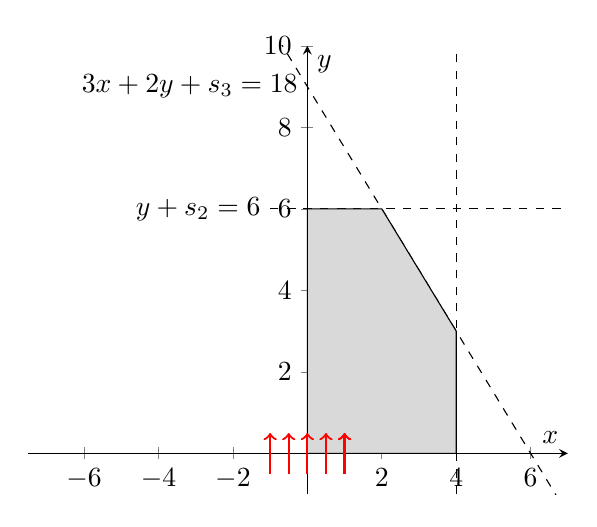
\begin{tikzpicture}
\begin{axis}[
  axis lines=middle,
  xmin=-7.5, xmax=7,
  ymin=-1, ymax=10,
  % xtick=0...20,
  % ytick=0...20,
  xlabel={$x$}, ylabel={$y$},
]
\addplot[black, dashed, domain=-1:7] {6};
\addplot[black, dashed, domain=-1:7] {-1.5*x + 9};
\addplot[black, dashed] coordinates {(4, -1) (4, 10)}; % vertical line x=4
\addplot[black, fill=gray!30] coordinates {(0,0) (0,6) (2,6) (4,3) (4,0) (0,0)};
\addplot[red, thick, ->] coordinates {(-1,-0.5) (-1,0.5)};
\addplot[red, thick, ->] coordinates {(-0.5,-0.5) (-0.5,0.5)};
\addplot[red, thick, ->] coordinates {(-0,-0.5) (-0,0.5)};
\addplot[red, thick, ->] coordinates {(0.5,-0.5) (0.5,0.5)};
\addplot[red, thick, ->] coordinates {(1,-0.5) (1,0.5)};
\addplot[red, thick, ->] coordinates {(1,-0.5) (1,0.5)};
\addplot[] coordinates {(-1, 6)}
node[pos=0.7, anchor=east] {$y+s_2 = 6$};
\addplot[] coordinates {(0, 9)}
node[pos=0.7, anchor=east] {$3x+2y+s_3 = 18$};
\end{axis}
\end{tikzpicture}
\end{center}

ณ ขั้นตอนนี้ เราทราบแล้วว่าเรากำลังจะเอาตัวแปร $y$ เข้ามาเป็นตัวแปรฐานใหม่ เพราะการเดินตามแนวแกน $y$ ให้การเปลี่ยนค่า $z$ ได้มากที่สุด
ซึ่งจากรูปภาพเราจะเห็นว่าจะมีเพียงขอบด้านซ้าย (เดินไปตามแกน $y$) เท่านั้นที่เป็นเส้นทางการเดินเดียวจากจุด $(0,0)$

คำถามต่อมาคือเดินควรไกลแค่ไหนถึงจะมั่นใจได้ว่าเดินไปถึงจุดมุมของบริเวณแน่ ๆ
ซึ่งถ้าเดินสั้นไปจะเดินไม่ถึงจุดมุม แต่ถ้าเดินไกลไปก็จะเลยจุดมุม
เพราะฉะนั้น เราจึงใช้ตัวแปรส่วนขาดเป็นตัวบอกว่าขอบของตัวแปรส่วนขาดใดอยู่ใกล้ที่สุด (ในกรณีอื่นอาจมีได้หลายเส้นทาง แต่เราก็จะเลือกอันที่ใกล้ที่สุดอยู่)
หรือกล่าวคือ เรากำลังจำลองว่าจะต้องเปลี่ยนค่า $y$ เท่าไหร่เพื่อให้ตัวแปรส่วนขาดของเส้นดังกล่าวมีค่าเป็น 0
\begin{example}
    {การเลือกตัวแปรเพื่อออกจากฐาน}{}
    จากรูปจะเห็นว่าถ้าเราเดิน จะไปพบได้ 2 เส้นเท่านั้นคือเส้นของ $s_2$ และเส้นของ $s_3$ จงหาค่า $y$ ของแต่ละเส้นที่ทำให้ตัวแปรส่วนขาดของเส้นดังกล่าวมีค่าเป็น 0 (สุดท้ายจะได้ว่าต้องเดินไปเส้นของ $s_2$)
    และเราจะสามารถเขียนแสดงผลลัพธ์ดังกล่าวในรูปแบบ simplex tableau ได้อย่างไร 
\end{example}
\newpage

\subsubsection*{ขั้นที่ 5: ทำ Pivot Row Operation เพื่ออัปเดต Tableau}

\begin{center}
    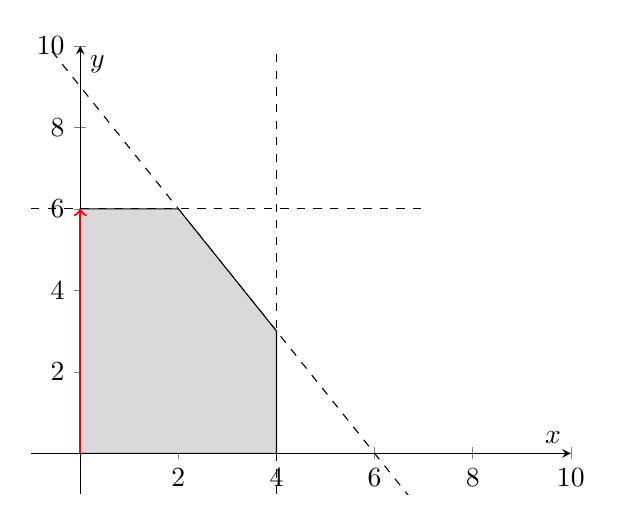
\begin{tikzpicture}
\begin{axis}[
  axis lines=middle,
  axis on top=false,
  xmin=-1, xmax=10,
  ymin=-1, ymax=10,
  % xtick=0...20,
  % ytick=0...20,
  xlabel={$x$}, ylabel={$y$},
]
\addplot[black, dashed, domain=-1:7] {6};
\addplot[black, dashed, domain=-1:7] {-1.5*x + 9};
\addplot[black, dashed] coordinates {(4, -1) (4, 10)}; % vertical line x=4
\addplot[black, fill=gray!30] coordinates {(0,0) (0,6) (2,6) (4,3) (4,0) (0,0)};
\addplot[red, thick, ->] coordinates {(0,0) (0,6)};
\end{axis}
\end{tikzpicture}
\end{center}

ตามความหมายในวิชาพีชคณิตเชิงเส้นเรื่องการแก้ระบบสมการเชิงเส้นนั้น pivot หมายถึงคอลัมน์ในเมทริกซ์สัมประสิทธิ์ที่มีสมาชิกเป็น 1 อยู่ตัวเดียว (เรียกว่า pivot element) และที่เหลือเป็น 0 ล้วน โดยในแต่ละแถวจะมี pivot element ได้ไม่เกิน 1 ตัว ซึ่งจากการที่เราบังคับให้ $s_2$ ออกจากการเป็นฐาน และนำ $y$ เข้ามาเป็นฐานแทน $s_2$ จึงต้องการให้ตาราง simplex อันใหม่มีหน้าตาดังนี้
    \begin{center}
    \renewcommand{\arraystretch}{1.4}
        \begin{tabular}{|c|ccccc|c|}
            \hline
            \textbf{Pivot} & $x$ & $y$ &  $s_1$ & $s_2$ & $s_3$ & \textbf{RHS} \\
            \hline
            $s_1$ & $*$ & $*$  & $1$ & $0$ & $0$ & $*$ \\
            $s_2$ & $*$ & $*$  & $0$ & $1$ & $0$ & $*$ \\
            $s_3$ & $*$ & $*$  & $0$ & $0$ & $1$ & $*$ \\
            \hline
            $z$   & $*$ & $*$  & $0$ & $0$ & $0$ & $*$ \\
            \hline
        \end{tabular}
        $\Longrightarrow$
        \begin{tabular}{|c|ccccc|c|}
            \hline
            \textbf{Pivot} & $x$ & $y$ &  $s_1$ & $s_2$ & $s_3$ & \textbf{RHS} \\
            \hline
            $s_1$ & $*$ & $0$  & $1$ & $*$ & $0$ & $*$ \\
            $y$   & $*$ & $1$  & $0$ & $*$ & $0$ & $*$ \\
            $s_3$ & $*$ & $0$  & $0$ & $*$ & $1$ & $*$ \\
            \hline
            $z$   & $*$ & $0$  & $0$ & $*$ & $0$ & $*$ \\
            \hline
        \end{tabular}
    \end{center}

\begin{example}
    {การเปลี่ยน pivot ของระบบ}{}
    แปลง simplex tableau ให้เป็นของระบบ pivot $s_1$, $y$ และ $s_3$ และให้เหตุผลว่าทำไมระบบปัจจุบันถึงแสดงสถานะว่ากำลังยืนอยู่ที่จุด $(0,6)$
\end{example}
\newpage
\subsubsection*{ขั้นที่ 6: วนซ้ำขั้นที่ 3-5 จนกว่าจะไม่มีสัมประสิทธิ์ติดลบในแถวของ $z$}
\begin{example}
    {ทำต่อ}{}
    ทำขั้นตอนที่ 3-5 วนจนกว่าจะจบกระบวนการ และแปลผลตารางสุดท้าย (ขั้นที่ 7)
\end{example}
\newpage
\begin{example}
    {}{}
    ใช้วิธี simplex หาผลเฉลยของกำหนดการเชิงเส้น
    \begin{align*}
        \max \quad & 4x + 2y \\
        \text{subject to} \quad
        & x \geq 0, \quad y \geq 0 \\
        & x \leq 2 \\
        & y \leq 3 \\
        & x - y \leq 1\\
        & x + y \leq 4
    \end{align*}
\end{example}
\newpage

\subsubsection{กรณีที่ 2: เงื่อนไขมี $\geq$ ที่อาจจะทำให้จุดกำเนิดไม่เป็น basic feasible solution}
ในบางกรณี เราอาจพบเงื่อนไขที่ทำให้จุดกำเนิดไม่ใช่ feasible solution เลยทำให้ไม่สามารถดำเนินการ simplex ได้ทันทีเหมือนกรณีที่ 1
ซึ่งกรณีดังกล่าวคือกรณีที่อสมการเงื่อนไขเขียนในรูป $ax + by \geq c$ โดยที่ $c \geq 0$ ซึ่งจะเห็นได้โดยง่ายว่าจุด $(0,0)$ ไม่เป็น feasible solution สำหรับเงื่อนไขนี้
แต่ถึงแม้เราจะใช้วิธีการการเพิ่มตัวแปรส่วนขาดเข้าไป ตัวอย่างเช่นสมการ $-3x + 5y \geq 4$ เมื่อเราทำการเพิ่มตัวแปรส่วนขาดเข้าไป จะได้สมการเป็น $-3x + 5y = 4 + s$ เมื่อ $s \geq 0$ หรือก็คือสมการ $-3x + 5y - s = 4$\footnote{หนังสือบางเล่มจะเรียกว่า\textbf{ตัวแปรส่วนเกิน} เพราะมองในลักษณะ $-3x + 5y - s = 4$ โดยที่ $s$ เป็นส่วนเกินของฝั่งที่มีค่ามากกว่า ทำให้เราต้องลบออกเพื่อให้ได้สมการ แต่ในมุมของผู้เขียนจะขอมองในลักษณะของตัวแปรส่วนขาดทั้งหมด แล้วใช้การย้ายข้างสมการแทน}
ซึ่งจะเห็นว่าถ้าให้ $x=0$ และ $y=0$ แล้วจะได้ว่า
$$
4 = -3x + 5y - s = -s \Longrightarrow s = -4 \ngeq 0
$$
กล่าวคือ เราไม่สามารถให้ $x$ และ $y$ เป็นตัวแปร non-basic ได้เหมือนกรณีที่ 1 

วิธีแก้ปัญหาคือเราจะเพิ่มตัวแปรเข้าระบบไปอีกตัว เพื่อปรับดุลสมการให้สามารถเริ่ม basic feasible solution ที่จุดกำเนิดได้ ซึ่งตัวแปรที่ถูกเพิ่มเข้ามานี้ถูกเรียกว่า \textbf{ตัวแปรจำลอง} (artificial variable) โดยจะได้สมการตัวอย่างเป็น
$$
-3x + 5y - s + A = 4 \text{ โดยที่ } A\geq 0
$$
และจะให้ตัวแปรจำลองเป็นตัวแปรพื้นฐาน และ $x,y,s$ มีค่าเป็น 0
โดยในขั้นตอนนี้ เราได้ basic feasible solution เริ่มต้นเป็นตัวแปรจำลอง ($A$) ซึ่งมีค่าเป็นบวก (ในที่นี้คือ $A=4$)  
แต่เป้าหมายของเราในการทำ Simplex method คือการกำจัดตัวแปรจำลองออกไปจากระบบในที่สุด เพราะตัวแปรจำลองนี้ไม่ได้มีความหมายในทางปฏิบัติ แต่เป็นเพียงตัวช่วยชั่วคราวในการเริ่มต้นหาคำตอบที่เหมาะสมที่สุดของระบบสมการ

การดำเนินการจากนี้เรียกกันโดยทั่วไปว่า \textbf{Simplex Method ระยะที่หนึ่ง (Phase I Simplex Method)} ซึ่งมีขั้นตอนการดำเนินงานดังต่อไปนี้:

\begin{enumerate}
    \item หลังจากเพิ่มตัวแปรจำลองในแต่ละสมการที่มีเงื่อนไข $\geq$ เรียบร้อยแล้ว เราจะกำหนดฟังก์ชันวัตถุประสงค์ชั่วคราว (Phase I Objective) ให้เป็นการหาผลรวมของตัวแปรจำลองทั้งหมดที่ถูกเพิ่มเข้าไป และเป้าหมายของขั้นตอนนี้คือการทำให้ผลรวมของตัวแปรจำลองมีค่าเท่ากับศูนย์ให้ได้ กล่าวคือเราสร้างฟังก์ชันวัตถุประสงค์ชั่วคราว (Phase I Objective) ดังนี้:
\[
\text{Minimize}\quad W = \sum (\text{ตัวแปรจำลองทั้งหมด})
\]

สำหรับตัวอย่างนี้จะได้เป็น
\[
\text{Minimize}\quad W = A
\]

    \item ใช้วิธี Simplex กับฟังก์ชันวัตถุประสงค์ชั่วคราวนี้ (Minimize $W$) และดำเนินการแปลงแถว (Pivot) ไปเรื่อย ๆ จนกว่าจะได้ตัวแปรจำลองจะออกจากฐานทั้งหมด

\begin{itemize}
    \item หากสามารถทำให้ฟังก์ชันวัตถุประสงค์ชั่วคราว $W=0$ ได้สำเร็จ แสดงว่าปัญหานี้มี feasible solution เดิมจริง และสามารถไปสู่ขั้นตอน Phase II ได้
    \item หากไม่สามารถทำให้ $W=0$ ได้ (เช่น $W>0$ เสมอ) แสดงว่าปัญหานี้ไม่มี feasible solution (infeasible problem) ไม่จำเป็นต้องดำเนินการต่อ
\end{itemize}

    \item เมื่อได้ $W=0$ แล้ว (กำจัดตัวแปรจำลองหมดแล้ว) เราจะดำเนินการต่อในขั้นที่สอง (\textbf{Phase II}) โดยกลับไปใช้ฟังก์ชันวัตถุประสงค์จริงของปัญหาเดิม และเริ่มทำ Simplex method ตามปกติจนได้คำตอบสุดท้าย
\end{enumerate}

\noindent
สรุปได้ว่าในกรณีที่ 2 นี้ การใช้ตัวแปรจำลอง (Artificial variable) และวิธีการ Simplex Phase I จะช่วยให้เราสามารถเริ่มต้นแก้ปัญหาการกำหนดการเชิงเส้นได้ แม้ว่าเงื่อนไขของปัญหาจะทำให้จุดกำเนิดไม่สามารถเป็น basic feasible solution ตั้งต้นได้ก็ตาม

\begin{example}
    {}{}
    ใช้วิธี simplex หาผลเฉลยของกำหนดการเชิงเส้น
    \begin{align*}
        \max \quad & 4x + 5y \\
        \text{subject to} \quad
        & x \geq 0, \quad y \geq 0 \\
        & -3x + 5y \geq 4\\
        & x + 2y \leq 8
    \end{align*}
\end{example}
\begin{solution}
    \begin{enumerate}[label=\textbf{ขั้นที่ \arabic*:}, align=left, labelwidth=5em, labelsep=1em, leftmargin=*, itemsep=16pt, topsep=0pt, parsep=0pt, partopsep=0pt]
    \item ปรับสมการให้อยู่ในรูปมาตรฐาน
        \begin{itemize}
            \item เนื่องจาก $(0,0)$ \textbf{ไม่}สอดคล้องเงื่อนไข $-3x + 5y \geq 4$ (แทนค่าแล้วได้ $0\geq 4$ ซึ่งเป็นเท็จ) เป็นจริง ดังนั้นจึงต้องเติมตัวแปรส่วนเกินและตัวแปรจำลอง ได้เป็น $-3x + 5y - s_1 + a_1 = 4$ โดยที่ $s_1, a_1 \geq 0$ โดยที่ให้ $a_1$ เป็นตัวแปรฐาน และ $x,y,s_1 = 0$ ในขั้นตั้งต้น
            \item เนื่องจาก $(0,0)$ สอดคล้องเงื่อนไข $3x + 2y \leq 8$ (แทนค่าแล้วได้ $0 \leq 8$ ซึ่งเป็นจริง) ดังนั้นจึงเติมตัวแปรส่วนขาดเข้าไปเท่านั้น ได้เป็น $x + 2y + s_2 = 8$ โดยที่ให้ $s_2$ เป็นตัวแปรฐานและ $x,y=0$
        \end{itemize}
        และเนื่องจากว่ามีตัวแปรจำลอง จึงต้องตั้งฟังก์ชันจุดประสงค์ชั่วคราวมให้เป็นการหาค่าต่ำสุดของผลรวมตัวแปรจำลอง กล่าวคือ $\min a_1$ แต่เนื่องจากเรากำลังจะทำ simplex จึงต้องปรับปัญหาให้เป็นการหาค่าสูงสุดด้วยการคูณ $-1$ เข้าไปได้เป็น $\max W = -a_1$ จึงได้ปัญหา Phase 1 ออกมาเป็น
        \begin{align*}
            \max \quad & W = -a_1 \\
            \text{subject to} \quad
            & x, y, s_1, s_2, a_1 \geq 0 \\
            & -3x + 5y -s_1 + a_1 = 4\\
            & x + 2y + s_2 = 8
        \end{align*}

    \newpage
    \item ตั้งตารางซิมเพล็กซ์ของตัวแปรจำลอง ได้เป็น
    \begin{center}
        \begin{tabular}{|c|ccccc|c|}
            \hline
            \textbf{Pivot} & $x$ & $y$ &  $s_1$ & $s_2$ & $a_1$ &  \textbf{RHS}  \\
            \hline
            $a_1$ & $-3$ & $5$  & $-1$ & $0$ & $1$ & $4$ \\
            $s_2$ & $1$ & $2$  & $0$ & $1$ & $0$ & $8$ \\
            \hline
            $W$   & $0$ & $0$  & $0$ & $0$ & $1$ & $0$ \\
            \hline
        \end{tabular}
    \end{center}
    และทำการกำจัดตัวแปรจำลองออกจากจุดประสงค์ (การเอาตัวแปรอื่นมาพิจารณา) เพื่อให้คอลัมน์ $a_1$ มีแถวของ $a_1$ เป็น 1 เพียงคนเดียว (เป็น pivot element ที่ตำแหน่งอื่นเป็น 0 ล้วน) ซึ่งทำได้โดยดำเนินการตามแถว $(-1)R_1 + R_3 \rightarrow R_3$ จะได้สมาชิกในแถวที่ $R_3$ ใหม่คำนวณได้ดังนี้
    \begin{itemize}
        \item คอลัมน์ $x$: $(-1)(-3) + 0 = 3$
        \item คอลัมน์ $y$: $(-1)(5) + 0 = -5$
        \item คอลัมน์ $s_1$: $(-1)(-1) + 0 = 1$
        \item คอลัมน์ $s_2$: $(-1)(0) + 0 = 0$
        \item คอลัมน์ $a_1$: $(-1)(1) + 1 = 0$
        \item คอลัมน์ $RHS$: $(-1)(4) + 0 = -4$
    \end{itemize}
    จึงได้ตารางซิมเพล็กซ์ตั้งต้นดังนี้ \textbf{(ถ้าในข้อสอบถามหาตารางตั้งต้น ต้องตอบตารางนี้ เพราะำคอลัมน์ $a_1$ ในตารางก่อนหน้ายังไม่อยู่ในรูปแบบ Pivot column)}
    \begin{center}
        \begin{tabular}{|c|ccccc|c|}
            \hline
            \textbf{Pivot} & $x$ & $y$ &  $s_1$ & $s_2$ & $a_1$ &  \textbf{RHS}  \\
            \hline
            $a_1$ & $-3$ & $5$  & $-1$ & $0$ & $1$ & $4$ \\
            $s_2$ & $1$ & $2$  & $0$ & $1$ & $0$ & $8$ \\
            \hline
            $W$   & $3$ & $-5$  & $1$ & $0$ & $0$ & $-4$ \\
            \hline
        \end{tabular}
    \end{center}
    \begin{remark}{การหาแถว $W$ อีกแบบ}{}
        เราสามารถหาแถว $W$ ได้แบบเร็วๆ โดยการนำสมการเงื่อนไขที่มีตัวแปรจำลองมาจัดรูปให้ตัวแปรจำลองอยู่ฝั่งหนึ่ง และตัวแปรที่เหลืออยู่อีกฝั่ง แล้วนำไปแทนค่าใน $W$ เช่นในเงื่อนไขที่ 1 ของตัวอย่างนี้คือ $-3x + 5y -s_1 + a_1 = 4$ และจัดรูปได้เป็น $a_1 = 3x - 5y + s_1 + 4$ แล้วนำไปแทนใน $W$ จะได้
        $$
        W = -a_1 = - (3x - 5y + s_1 + 4) = -3x + 5y - s_1 -4
        $$
        และย้ายข้างได้รูปแบบ $W +3x - 5y + s_1 = -4$ ทำให้เขียนสัมประสิทธิ์ได้เป็น $$3\quad-5\quad1\quad0\quad0\quad|\quad-4$$
    \end{remark}

    และทำกระบวนการ simplex ไปจนกว่าตัวแปรจำลองจะออกจากตัวแปรฐานทั้งหมด โดยจากตารางจะได้ว่าต้องให้ $y$ เป็นตัวแปรเข้าฐาน และเมื่อหาอัตราส่วนเพื่อเลือกตัวแปรขาออกจากฐานตามตารางด้านล่าง จะได้ว่าต้องใช้ $a_2$ ออกจากฐาน

    \begin{center}
        \begin{tabular}{|c|ccccc|c|c|}
            \hline
            \textbf{Pivot} & $x$ & $y$ &  $s_1$ & $s_2$ & $a_1$ &  \textbf{RHS} & อัตราส่วน  \\
            \hline
            $a_1$ & $-3$ & $5$  & $-1$ & $0$ & $1$ & $4$ & $4/5= 0.8$ \\
            $s_2$ & $1$ & $2$  & $0$ & $1$ & $0$ & $8$ & $8/2= 4$ \\
            \hline
            $W$   & $3$ & $-5$  & $1$ & $0$ & $0$ & $-4$ & \\
            \hline
        \end{tabular}
    \end{center}

    ดำเนินการตามแถวเพื่อเปลี่ยน pivot โดยใช้ $R_1/5$, $(-2/5)R_1 + R_2 \rightarrow R_2 $ และ $(1)R_1 + R_3 \rightarrow R_3 $ จะได้
    \begin{center}
        \begin{tabular}{|c|ccccc|c|}
            \hline
            \textbf{Pivot} & $x$ & $y$ &  $s_1$ & $s_2$ & $a_1$ &  \textbf{RHS}  \\
            \hline
            $y$ & $-3/5$ & $1$  & $-1/5$ & $0$ & $1/5$ & $4/5$ \\
            $s_2$ & $11/5$ & $0$  & $2/5$ & $1$ & $-2/5$ & $32/5$ \\
            \hline
            $W$   & $0$ & $0$  & $0$ & $0$ & $1$ & $0$ \\
            \hline
        \end{tabular}
    \end{center}
    ซึ่งตารางใหม่ไม่สามารถอัพเดตเพิ่มเติมได้อีกแล้ว และตัวแปรจำลองถูกกำจัดออกจากตัวแปรฐานได้ทั้งหมด และได้ $W=0$ จึงได้ว่าสามารถทำ simplex phase 2 ต่อได้โดยใช้ชุดสัมประสิทธิ์ที่ได้จาก phase 1
    \begin{center}
        \begin{tabular}{|c|cccc|c|}
            \hline
            \textbf{Pivot} & $x$ & $y$ &  $s_1$ & $s_2$ &  \textbf{RHS}  \\
            \hline
            $y$ & $-3/5$ & $1$  & $-1/5$ & $0$ & $4/5$ \\
            $s_2$ & $11/5$ & $0$  & $2/5$ & $1$ & $32/5$ \\
            \hline
            $z$   & $-4$ & $-5$  & $0$ & $0$ & $0$ \\
            \hline
        \end{tabular}
    \end{center}

    \begin{remark}{ความหมายของผลที่ได้จาก Phase 1}{}
        ผลที่ได้จากการทำ simplex phase 1 คือการพยายามหาจุดผลเฉลยตั้งต้น (basic feasible solution) ซึ่งจากเดิมเราสามารถเริ่มได้โดยง่ายที่จุด $x=0, y=0$ แต่ว่าในกรณีที่มีเงื่อนไขที่ทำให้จุดดังกล่าวไม่สอดคล้อง (เช่นเงื่อนไข $-3x + 5y \geq 4$) เราจึงจำเป็นต้องเพิ่มตัวแปรจำลองเพื่อจำลองการเดินทางจากจุด $(0,0)$ ไปที่จุดมุมตั้งต้นที่ใกล้ที่สุด ซึ่งจากตารางสุดท้ายที่ได้มาจาก phase 1 เราได้ระบบสมการ
        \begin{align*}
            -\frac{3}{5}x + y - \frac{1}{5}s_1 &= \frac{4}{5}\\
            \frac{11}{5}x + \frac{2}{5}s_1 + s_2 &= \frac{32}{5}
        \end{align*}
        โดยที่ $x = 0, s_1=0$ (เพราะไม่ใช่ฐาน) ซึ่งเมื่อแก้ระบบสมการหาค่าตัวแปรฐาน จะได้ $y=4/5$ และ $s_2 = 32/5$ ซึ่งหมายถึง เราหาจุดผลเฉลยตั้งต้นได้เป็นจุด $(x,y) = (0, 4/5)$ และใช้ระบบของจุดนี้เพื่อไปแก้หาค่าสูงสุดของ $Z$ ต่อได้
    \end{remark}
    
    \item ดำเนินการ simplex ได้ตามปกติ (ทิ้งไว้ให้เป็นแบบฝึกหัดเพิ่มเติมเพื่อทบทวนการดำเนินการ simplex)
    \end{enumerate}
\end{solution}

\subsubsection{กรณีที่ 3: เงื่อนไขมี $=$ ซึ่งทำให้ feasible ไม่เป็น region เต็มมิติ}
\begin{example}
    {}{}
    ใช้วิธี simplex หาผลเฉลยของกำหนดการเชิงเส้น
    \begin{align*}
        \max \quad & 2x + 15y \\
        \text{subject to} \quad
        & x \geq 0, \quad y \geq 0 \\
        & -3x + 5y \leq 15\\
        & 2x + 5y \leq 40\\
        & 4x -5y = 20
    \end{align*}
\end{example}
\newpage
\begin{example}
    {โจทย์ผสม}{}
    ใช้วิธี simplex หาผลเฉลยของกำหนดการเชิงเส้น
    \begin{align*}
        \min \quad & -1840x - 1720y \\
        \text{subject to} \quad
        & x \geq 0, \quad y \geq 0 \\
        & 2x+y \leq 1800\\
        & 2x + 2y \geq 1400\\
        & x -2y = 100
    \end{align*}
\end{example}
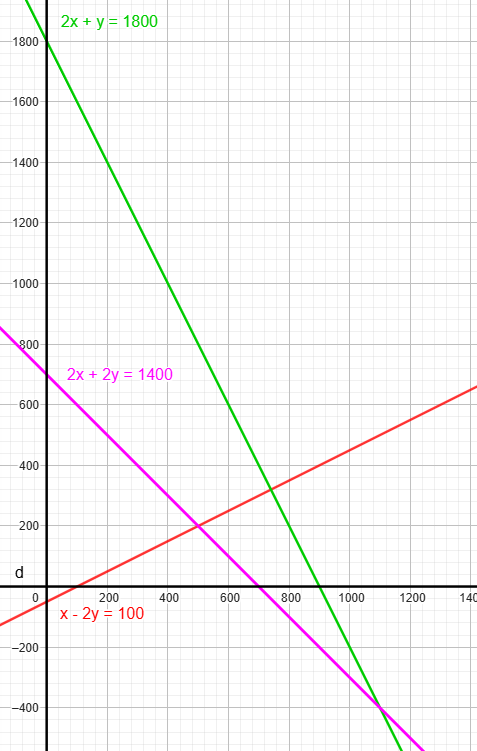
\includegraphics[width=0.5\linewidth]{ex-simplex-mix.png}


\newpage
\section{การแก้ปัญหาด้วย Excel Solver}

\subsection*{สถานการณ์จำลอง}
โรงงานผลิตน้ำผลไม้แห่งหนึ่งมีผลิตภัณฑ์ 4 ชนิด ได้แก่ น้ำส้ม (A), น้ำแอปเปิ้ล (B), น้ำองุ่น (C) และน้ำเสาวรส (D) โดยการผลิตแต่ละชนิดต้องใช้วัตถุดิบและเวลาที่แตกต่างกัน โรงงานมีข้อจำกัดด้านวัตถุดิบ วัตถุบรรจุ และแรงงานต่อวันตามตารางด้านล่าง

\begin{center}
\begin{tabular}{lcccc}
\toprule
\textbf{ทรัพยากร / ผลิตภัณฑ์} & \textbf{A (น้ำส้ม)} & \textbf{B (น้ำแอปเปิ้ล)} & \textbf{C (น้ำองุ่น)} & \textbf{D (น้ำเสาวรส)} \\
\midrule
วัตถุดิบ (ลิตร) & 2.0 & 1.5 & 2.2 & 1.0 \\
วัตถุบรรจุ (หน่วย) & 1.0 & 1.0 & 0.8 & 1.2 \\
แรงงาน (ชม.) & 0.5 & 0.7 & 0.6 & 0.4 \\
กำไรต่อหน่วย (บาท) & 10 & 8 & 12 & 9 \\
\bottomrule
\end{tabular}
\end{center}

ข้อจำกัดต่อวัน:
\begin{itemize}
    \item วัตถุดิบไม่เกิน 500 ลิตร
    \item วัตถุบรรจุไม่เกิน 250 หน่วย
    \item ชั่วโมงแรงงานไม่เกิน 120 ชั่วโมง
\end{itemize}

\subsection*{คำสั่งในการทำงาน}
\begin{enumerate}[label=\arabic*.]
    \item กำหนดให้ตัวแปร $x_1, x_2, x_3, x_4$ แทนจำนวนหน่วยของ A, B, C, D ตามลำดับ
    \item เขียนแบบจำลองทางคณิตศาสตร์ในรูปแบบ LP โดยกำหนด
    \begin{itemize}
        \item \textbf{ฟังก์ชันวัตถุประสงค์:} Maximize กำไรรวม
        \item \textbf{ข้อจำกัด:} ทรัพยากรไม่เกินที่กำหนด
        \item \textbf{เงื่อนไข:} $x_1, x_2, x_3, x_4 \geq 0$
    \end{itemize}
    \item เปิด Excel และสร้างตารางการคำนวณ (Decision Variables, Total Usage, Constraints)
    \item ใช้ \textbf{Solver} เพื่อหาคำตอบที่ให้กำไรสูงสุด โดยกำหนดเงื่อนไขที่เหมาะสม
    \item บันทึกผลลัพธ์ที่ได้
\end{enumerate}

\subsection*{คำถามท้ายแล็บ}
\begin{enumerate}[label=\alph*.]
    \item ผลลัพธ์ที่ได้คือ: $x_1 = \_\_\_$, $x_2 = \_\_\_$, $x_3 = \_\_\_$, $x_4 = \_\_\_$ และกำไรสูงสุดคือ \_\_\_ บาท
    \item ข้อจำกัดใดที่ใช้เต็มความสามารถ? และข้อจำกัดใดที่ยังมีทรัพยากรเหลือ?
    \item หากโรงงานสามารถเพิ่มแรงงานได้อีก 10 ชั่วโมง จะส่งผลต่อกำไรหรือไม่?
    \item หากบริษัทต้องการผลิตแบบจำนวนเต็ม จะต้องเปลี่ยนการตั้งค่า Solver อย่างไร?
\end{enumerate}
\newpage
% \section{หัวข้อพิเศษ: ปัญหาอื่น ๆ ที่เป็นรูปแบบกำหนดการเชิงเส้น}
% \subsection{Transportation Problem}
% \subsection{Scheduling Problem}
% \subsection{Assignment Problem}

% \newpage
\section*{Assignment}

จากสถานการณ์ของบริษัท ABC Furniture ที่ต้องการวางแผนการผลิต “โต๊ะทำงาน” และ “ตู้เก็บเอกสาร” เพื่อให้ได้ยอดสูงสุดภายใต้ข้อจำกัดของแรงงานและวัตถุดิบ (ตามสถานการณ์ในต้นบท)

\subsection*{Part A: การสร้างโมเดลคณิตศาสตร์}
\begin{enumerate}
    \item จากสถานการณ์ของบริษัท ABC Furniture
        \begin{enumerate}
            \item กำหนดตัวแปรให้ชัดเจน
            \item เขียนสมการจุดประสงค์ (Objective Function)
            \item เขียนข้อจำกัดทั้งหมด (Constraints)
            \item ระบุ Domain ของตัวแปร
        \end{enumerate}
\end{enumerate}
\begin{solution}
    เนื่องจากเราต้องวางแผนจำนวนการผลิตโต๊ะทำงานและตู้เก็บเอกสาร ดังนั้นเราจึงต้องกำหนดตัวแปรเป้นจำนวนโต๊ะและจำนวนตู้ โดยในที่นี้ กำหนดให้
    \begin{align*}
        x &= \text{จำนวนโต๊ะทำงานที่จะผลิต}\\
        y &= \text{จำนวนตู้เก็บเอกสารที่จะผลิต}
    \end{align*}

    เป้าหมายของการผลิตคือเพื่อที่ทำให้ได้ยอดขายสูงที่สุด ดังนั้นจึงต้องวางฟังก์ชันจุดประสงค์คือยอดขาย และเนื่องจากยอดขายคิดได้จากจำนวนโต๊ะและจำนวนตู้ที่ผลิตคูณด้วยราคาที่ขายตรง ๆ จึงได้ว่า สมการจุดประสงค์คือยอดขาย
    $$
    2000x + 1500y
    $$

    ในส่วนของเงื่อนไขที่เป็นข้อจำกัดของโจทย์นี้จะมีเรื่องของเวลาแรงงานและปริมาณวัตถุดิบที่มี
    \begin{itemize}
        \item การผลิตโต๊ะ $x$ ตัวซึ่งต้องใช้เวลาผลิตตัวละ 4 ชั่วโมง จึงต้องใช้เวลาผลิตโต๊ะทั้งหมด $4x$ ชั่วโมง
        \item การผลิตตู้ $y$ ตัวซึ่งต้องใช้เวลาผลิตตัวละ 3 ชั่วโมง จึงต้องใช้เวลาผลิตโต๊ะทั้งหมด $3y$ ชั่วโมง
    \end{itemize}
    ดังนั้นเราจึงใช้เวลาแรงงานในการผลิตทั้งหมด $4x + 3y$ และเพราะเรามีเวลาจำกัดสูงสุดที่ 1000 ชั่วโมง จึงได้เงื่อนไขด้านเวลาเป็น
    $$
    4x + 3y \leq 1000
    $$
    ในทำนองเดียวกัน เราจะได้เงื่อนไขเรื่องวัตถุดิบเป็น
    $$
    2x + y \leq 800
    $$

    ทั้งนี้ เนื่องจากตัวแปรที่เราตั้งไว้เป็นเรื่องของจำนวนการผลิต ดังนั้น Domain ของจำนวนแปรจึงคือจำนวนเต็มที่ไม่เป็นลบ (ถึงแม้ตอนเราแก้ปัญหาเราจะสนใจแค่ไม่ติดลบอย่างเดียวก็ตาม: $x \geq 0, y\geq 0$)

    สรุปแล้ว โจทย์นี้เราจะได้แบบจำลองกำหนดการเชิงเส้นอยู่ในรูป
        \begin{align*}
            \max \quad & 2000x + 1500y \\
            \texttt{subject to} \quad
            & 4x + 3y \leq 1000 \\
            & 2x + y \leq 800 \\
            & x \geq 0, \quad y \geq 0 
        \end{align*}
\end{solution}

\subsection*{Part B: การวิเคราะห์และคำนวณผลลัพธ์}
\begin{enumerate}
    \item หาผลเฉลยด้วยวิธีการวาดกราฟ
    \begin{solution}
        เริ่มจากการหาจุดตัดแกนของแต่ละเส้นสมการเงื่อนไข
        \begin{center}
            \begin{tabular}{|c|c|c|}
                \hline
                    สมการ & จุดตัดแกน $x$ (แทน $y=0$)  & จุดตัดแกน $y$ (แทน $x=0$) \\
                    \hline
                    $4x + 3y= 1000$ & $4x = 1000 \Rightarrow x = 250$ & $3y = 1000 \Rightarrow y = 1000/3 \approx 333.33$ \\
                    \hline
                    $2x + y = 800$ & $2x = 800 \Rightarrow x = 400$ & $y = 800$\\
                    \hline
            \end{tabular}\\
    
            
            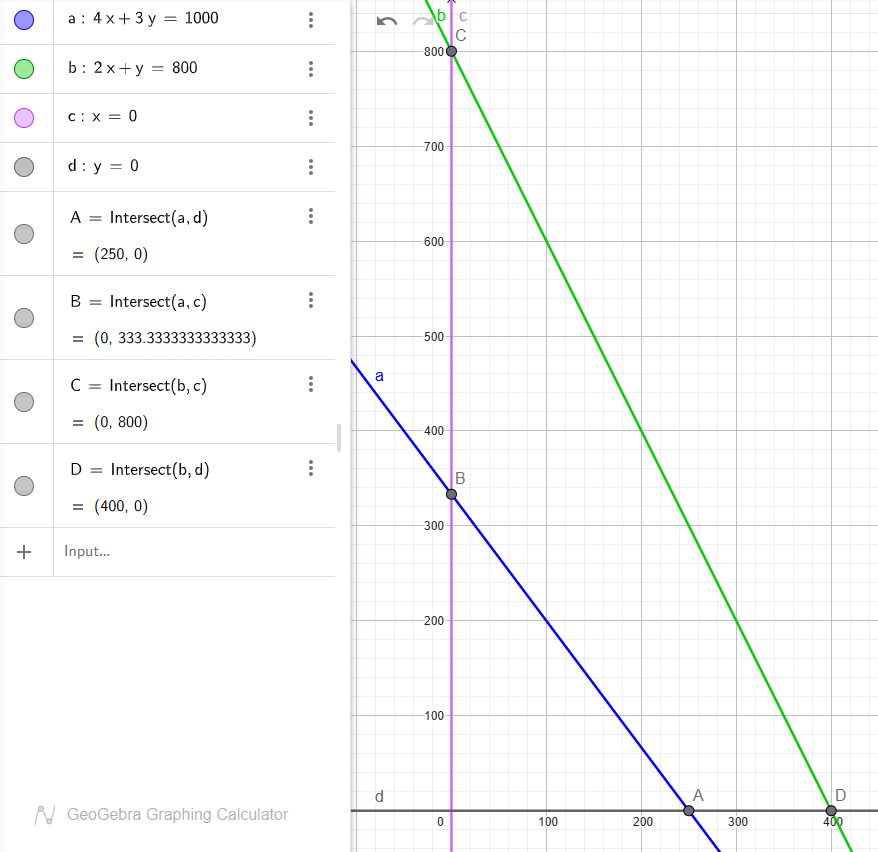
\includegraphics[width=0.6\linewidth]{assChap1-B-1.png}
        \end{center}
        จะได้ว่าบริเวณความเป็นไปได้ (feasible region) คือรูปสามเหลี่ยมที่ปิดล้อมด้วยแกน $x$, แกน $y$ และเส้นตรงสมการ $4x+3y=1000$ ซึ่งมีจุดยอด 3 จุดได้แก่ $(0,0), (0,1000/3), (250,0)$ (เนื่องจากในข้อนี้ไม่มีการตัดกันของเส้นสมการเงื่อนไขในบริเวณที่สนใจ จึงไม่มีการแก้ระบบสมการเพื่อหาจุดตัด)
    
        สุดท้ายคือแทนค่าจุดมุมลงในฟังก์ชันจุดประสงค์เพื่อหาค่าแล้วเปรียบเทียบกันว่าจุดใดให้ค่าจุดประสงค์มากที่สุด
    
        \begin{center}
            \begin{tabular}{c|c}
                $(x,y)$ & $\text{ยอดขาย} = 2000x + 1500y$ \\
                \hline
                $(0,0)$ & 0 \\
                \hline
                $(0,1000/3)\approx(0,333)$ & $499500$ \\
                \hline
                $(250,0)$ & $500000$ \\
                \hline
            \end{tabular}
        \end{center}
        ซึ่งทำให้ได้ว่าค่ายอดขายสูงสุดที่จะทำได้ภายใต้เงื่อนไขที่กำหนดมาคือ $500,000$ บาท ที่จะผลิตโต๊ะอย่างเดียว $250$ ตัว
        \begin{remark}
            {}{}
            ถ้าไม่นับเรื่องการปัดให้เป็นจำนวนเต็มนั้น จริงๆ แล้วที่จุด $(0,1000/3)$ ก็ให้ค่ายอดขายสูงสุดเป็น $500000$ บาทเช่นกัน แต่ว่าเนื่องจากเราต้องปัดให้เป็นจำนวนเต็ม และไม่สามารถปัดขึ้นได้เนื่องจากจะเกินเงื่อนไขที่กำหนดมา ทำให้เราสามารถผลิตได้ยอดขายแค่ $499500$ ที่จุดที่จะผลิตตู้อย่างเดียว\\
    
            นอกจากนั้น ทุกจุดบนเส้นสมการเงื่อนไข $4x+3y=1000$ นั้นต่างให้ค่าฟังก์ชันจุดประสงค์เป็น $500000$ เหมือนกันทุกจุด (เป็นโจทย์ทิ้งไว้ให้นักศึกษาลองคิดว่าทำไมถึงเป็นเช่นนั้น) ดังนั้น เราอาจจะเลือกตัวเลือกอื่นที่ไม่ใช่จุดมุมก็ได้ ตราบใดที่ยังเป็นจุดที่ทั้ง $x$ และ $y$ ต่างเป็นจำนวนเต็มและยังอยู่บนเงื่อนไขดังกล่าว (ตัวอย่างเช่น $x = 100, y=250$ ก็เป็นอีกจุดที่ยังสอดคล้องเงื่อนไขของโจทย์และให้ค่ายอดขายรวมเป็น $500000$ เช่นเดียวกัน)\\
    
            \textbf{โจทย์ Challenge}
            \begin{align*}
                \max \quad & 2000x + 1500y \\
                \texttt{subject to} \quad
                & 4x + 3y \leq 1000 \\
                & 2x + y \leq 800 \\
                & x \geq 0, \quad y \geq 0 
            \end{align*}
            \begin{enumerate}
                \item ทำไมทุกจุดบนเส้นเงื่อนไข $4x + 3y = 1000$ ถึงทำให้ค่ายอดขายรวมได้ราคา $500,000$ บาทเหมือนกันทั้งหมด
                \item ถ้าเกิดทางบริษัท ABC Furniture ไม่ต้องการตัวเลือกที่ผลิตแค่อย่างใดอย่างหนึ่งเท่านั้น แต่ให้ช่วยลิสต์รายการทั้งหมดที่เป็นไปได้ที่ทำให้ยอดขายรวมได้ $500,000$ บาทเหมือนกัน เราจะมีวิธีการหาตัวเลือกทั้งหมดนั้นอย่างไร\\
                (คำใบ้ $x = 250 - \frac{3}{4}y$)
            \end{enumerate}
        \end{remark}
    \end{solution}
    
    

    \item หาผลเฉลยด้วยวิธี Simplex method
    \item จงอธิบายความหมายทางเรขาคณิตของแต่ละ simplex tableau ที่ได้ในข้อที่ผ่านมา
    \item หาผลเฉลยด้วย Excel Solver
    \item ถ้าบริษัทเพิ่มแรงงานได้เป็น 1,200 ชั่วโมงต่อสัปดาห์ ข้อจำกัดเปลี่ยนแปลงอย่างไร และคำตอบใหม่คืออะไร?
    \item ถ้าราคาขายตู้เก็บเอกสารเพิ่มเป็น 1,800 บาท จะมีผลต่อคำตอบอย่างไร? ควรผลิตเปลี่ยนไปหรือไม่?
\end{enumerate}

\subsection*{Part C: Sensitivity Analysis}
เราสามารถลด (หรือเพิ่ม) ทรัพยากรได้แค่ไหน โดยที่คำตอบที่ดีที่สุด (optimal solution) ยังไม่เปลี่ยน?
\begin{enumerate}
    \item อธิบายเงื่อนไขเชิงเรขาคณิตที่ทำให้คำตอบที่เหมาะสมที่สุดยังคงอยู่ที่เดิม เมื่อเปลี่ยนค่าด้านขวาของข้อจำกัด (RHS)
    \item พิจารณาว่าเราสามารถลดค่าของ RHS ของข้อจำกัดแรงงาน (1000) และวัตถุดิบ (800) ลงอย่างละเท่าไร โดยที่จุดคำตอบเดิมยัง feasible และยังเป็นคำตอบที่ให้ค่า Z มากที่สุด
\end{enumerate}


	\chapter{ทฤษฎีการตัดสินใจ (Decision Theory)}

\section*{โจทย์ธุรกิจ}
\begin{tcolorbox}[colback=white!100!white, colframe=black!80!white,
  title=ข้อความ,
  fonttitle=\bfseries,
  sharp corners=southwest,
  boxrule=0.8pt,
  left=1mm, right=1mm, top=1mm, bottom=1mm,
]
\emph{
``ขอบคุณสำหรับแผนการผลิตที่คุณแนะนำครับ แต่เรายังมีปัญหาใหม่เกิดขึ้น...  
ฝ่ายบริหารกำลังลังเลว่าจะใช้กลยุทธ์ไหนต่อในไตรมาสหน้า  
เพราะสถานการณ์ตลาดมีแนวโน้มเปลี่ยนแปลงตลอดเวลา  
บางสัปดาห์โต๊ะทำงานขายดี บางสัปดาห์กลับเป็นตู้เอกสารที่มาแรง  
บางทีก็มีปัญหาขนส่งวัตถุดิบจากซัพพลายเออร์อีก  
ถ้าจะวางกลยุทธ์ที่เหมาะสม เราควรเลือกแนวทางการผลิตแบบใด?"}
\end{tcolorbox}
คุณสมชายกลับมาอีกครั้ง หลังจากบริษัท ABC Furniture ใช้แบบจำลองเชิงเส้นเพื่อตัดสินใจจำนวนการผลิตโต๊ะทำงานและตู้เก็บเอกสารในแต่ละสัปดาห์ได้แล้ว ซึ่งทำให้ได้ผลดีในช่วงแรก ๆ ที่ใช้งาน แต่ผ่านไปสักพักฝ่ายการตลาดพบว่ามีปัจจัยภายนอกมากระทบทำให้ไม่สามารถใช้แค่เกณฑ์ภายในด้านกำไรมาพิจารณาได้อย่างเดียว และสถานการณ์ตลาดเปลี่ยนแปลงอย่างรวดเร็ว — ทำให้ฝ่ายการผลิตต้องเผชิญกับความไม่แน่นอนหลายด้าน เช่น
\begin{itemize}
    \item ราคาขายเปลี่ยนแปลง
    \item ความต้องการของลูกค้าเปลี่ยนไป
    \item มีปัญหาการขนส่งวัตถุดิบ
    \item คู่แข่งออกรุ่นใหม่ที่มีราคาถูกกว่า
\end{itemize}~
เพื่อช่วยในการวางแผน บริษัทจึงอยากรู้ว่า หากมีสถานการณ์ที่ไม่แน่นอน (uncertain states of nature) เกิดขึ้น บริษัทควรเลือกแนวทางการผลิตแบบใดเพื่อรับมือ

\textbf{คำถามชวนคิด:}
\begin{itemize}
    \item คุณคิดว่าบริษัท ABC Furniture กำลังเผชิญกับปัญหาแบบใด? ทำไม LP ไม่ตอบโจทย์?
    \item คุณต้องการข้อมูลอะไรเพิ่มเติมก่อนจะตอบคำถามของคุณสมชายได้?
    \item คุณจะเริ่มต้นจัดกลุ่มหรือจำแนกทางเลือกในการตัดสินใจอย่างไร?
    \item หากไม่สามารถรู้อนาคตได้แน่ชัด คุณจะวิเคราะห์หรือวางแผนอย่างไร?
    \item ลองจินตนาการว่าบริษัทอาจมี “หลายสถานการณ์ตลาด” ที่อาจเกิดขึ้น คุณจะจัดโครงสร้างปัญหาเพื่อเปรียบเทียบตัวเลือกได้อย่างไร?
    \item คุณคาดหวังว่าข้อมูลลักษณะใดจะช่วยให้การตัดสินใจแม่นยำมากขึ้น?
\end{itemize}

\section*{บทนำ}
(Draft Version)\footnote{draft for teaching in class, not for text book this semester}

\begin{itemize}
    \item ในบางครั้ง ก็มีทางเลือกที่จะต้องตัดสินใจเลือก
    \item เป้าหมายคือทางเลือกที่ดีที่สุด
    \item แต่ก็มีรูปแบบของสถานการณ์ได้หลากหลาย ขึ้นกับการเกิดขึ้นของทางเลือกที่มี: (1) ภายใต้ความแน่นอน (2) ภายใต้ความเสี่ยง และ (3) ภายใต้ความไม่แน่นอน
    \item ซึ่งการตัดสินใจภายใต้ความเสี่ยงและความไม่แน่นอนนั้นจะใช้ทฤษฎีความน่าจะเป็นเข้ามาช่วย: ค่าคาดหวัง (expected value)
\end{itemize}

\section{ลักษณะการแสดงข้อมูล}
เราสามารถแสดงข้อมูลเพื่อความง่ายในการอ่านได้ 2 รูปดังนี้
\begin{enumerate}
    \item เมทริกซ์การตัดสินใจ (decision matrix) เป็นการแสดงผลจากลัพธ์ (เช่น กำไร) ระหว่างตัวเลือก (option) และเหตุการณ์ที่เป็นไปได้ที่อาจจะเกิดขึ้น
    \begin{center}
        \begin{tabular}{c|c|c|c|c|}
             & เหตุการณ์ 1 & เหตุการณ์ 2 & $\cdots$ & เหตุการณ์ $n$ \\ \hline
            ทางเลือก 1 &  & & & \\
            ทางเลือก 2 &  & & & \\
            $\vdots$ &  & & & \\
            ทางเลือก $m$ &  & & & \\ \hline
        \end{tabular}
    \end{center}
        
    \item ต้นไม้การตัดสินใจ (decision tree) เป็นลักษณะของการแสดงความต่อเนื่องของเหตุการณ์การเลือกโดยอาศัยจุดยอด (node) เชื่อมต่อกัน และปลายกิ่งสุดท้ายจะแสดงผลลัพธ์ที่เกิดขึ้น
    \begin{figure}[h!]
        \centering
        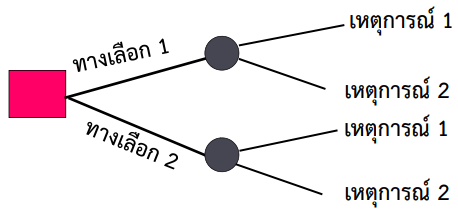
\includegraphics[width=0.5\linewidth]{decisiontree.png}
        \caption{Enter Caption}
        \label{fig:enter-label}
    \end{figure}
\end{enumerate}

\begin{example}
    {ตัวอย่างการสร้างเมทริกซ์การตัดสินใจ และต้นไม้การตัดสินใจ}{decision-matrix}
    ณ บริษัทสมมติแห่งหนึ่ง ต้องการตัดสินใจว่าจะจัดนิทรรศการขนาดเล็ก หรือขนาดกลาง หรือขนาดใหญ่ โดยจากการประเมิณเบื้องต้นพบว่าถ้าขายบัตรเข้างานได้หมด จะได้กำไร 8 ล้านบาท, 15 ล้านบาท และ 25 ล้านบาทเรียงตามขนาดของงาน ในขณะที่ถ้าขายได้ 50\% ของบัตรทั้งหมดจะได้กำไร 4 ล้านบาท, 15 ล้านบาท และ 10 ล้านบาทตามลำดับ และถ้าขายได้เพียงแค่ 10\% ของบัตรทั้งหมดจะได้กำไร 3 บาท และขาดทุน 1 ล้านบาทและ 10 ล้านบาทตามลำดับขนาดของงาน จากเหตุการณ์ดังกล่าว จะสร้างเมทริกซ์การตัดสินใจและต้นไม้การตัดสินใจได้ดังนี้
\end{example}
\newpage

\section{การตัดสินใจภายใต้สภาวะความแน่นอน}
\begin{itemize}
    \item เมื่อทราบว่าจะเกิดเหตุการณ์ใดขึ้น
    \item ถึงจะไม่ realistic ในหลาย ๆ กรณี แต่บางครั้งเราก็ต้องพิจารณาในรูปแบบนี้
    \item เพราะง่ายและตรงไปตรงมา
\end{itemize}

\begin{example}
    {การตัดสินใจภายใต้สภาวะความแน่นอน}{}
    จากเมทริกซ์การตัดสินใจที่ได้จากตัวอย่าง \ref{ex:decision-matrix} จะตัดสินใจภายใต้สภาวะความแน่นอนของแต่ละเหตุการณ์ได้อย่างไรบ้าง
\end{example}

\newpage
\section{การตัดสินใจภายใต้สภาวะความเสี่ยง}
\begin{itemize}
    \item ไม่ทราบว่าจะเกิดเหตุการณ์ใด
    \item แต่พอมีข้อมูลเพื่อคาดการณ์ความน่าจะเป็นของการเกิดแต่ละเหตุการณ์ได้
    \item ใช้แนวคิดเรื่องของความน่าจะเป็นเข้ามาช่วย
\end{itemize}
\subsection{ค่าคาดหวัง (Expected Value)}
\begin{definition}
    {ค่าคาดหวัง}{}
    ภายใต้การทดลองเชิงการสุ่มหนึ่ง ถ้าผลจอบแทนทั้งหมดที่เป็นไปได้คือ $X = X_1, X_2, X_3, \dots$ (อาจจะมีจำกัดหรือไม่จำกัดเหตุการณ์ก็ได้) โดยที่มีความน่าจะเป็นการได้ผลตอบแทนเป็น $P(X) = P(X_1), P(X_2), P(X_3), \dots$ ตามลำดับ
    แล้ว\textbf{ค่าคาดหวัง}ของผลตอบแทนจะคำนวณโดย
    $$
    E(X) := X_1 P(X_1) + X_2 P(X_2) + X_3 P(X_3) + \cdots
    $$
\end{definition}
ซึ่งค่าคาดหวังในเชิงความน่าจะเป็นเปรียบเสมือนค่าเฉลี่ยในเชิงสถิติที่จะบอกแนวโน้มการได้ว่ามักจะได้ค่าไหนเป็นส่วนใหญ่
\begin{example}
    {ค่าคาดหวังของเหตุการณ์อย่างง่าย}{}
    สมมติว่าพนันด้วยการโยนเหรียญไม่เที่ยงตรงอันหนึ่งโดยมีโอกาสออกหัว 0.3 และออกก้อย 0.7 ในการพนันนี้มีกฏว่าถ้าออกหัวผู้เล่นจะได้เงิน 5 บาท ในขณะที่ถ้าออกก้อยผู้เล่นจะเสียเงิน 3 บาท ในการเล่นพนันครั้งนี้ผู้เล่นจะเสียเปรียบหรือว่าได้เปรียบอยู่กี่บาท
\end{example}

\newpage
\subsection{เกณฑ์ผลตอบแทน}
\begin{example}
    {การตัดสินใจภายใต้สภาวะความเสี่ยง:ค่าคาดหวังของผลตอบแทน}{}
    จากเมทริกซ์การตัดสินใจที่ได้จากตัวอย่าง \ref{ex:decision-matrix} ซึ่งคือ
    \begin{center}
        \begin{tabular}{|c|c|c|c|}
        \hline
            (หน่วย: ล้านบาท) & ขายได้หมด & ขายได้ 50\% & ขายได้ 10\% \\ \hline
            ขนาดเล็ก & 8 & 4 & 3 \\
            ขนาดกลาง & 15 & 15 & -1\\
            ขนาดใหญ่ & 25 & 10 & -10\\ \hline
        \end{tabular}
    \end{center}
    และจากการสำรวจสถิติเก่า ๆ พบว่า โอกาสที่จะขายได้หมดมี 0.3 ในขณะที่ขายได้ครึ่งหนึ่งของงานจะมีโอกาสที่ 0.4 และขายได้เพียง 10\% ของงานจะมีโอกาสอยู่ที่ 0.3
    เนื่องจากเราไม่ทราบว่าจะเกิดเหตุการณ์แบบไหนขึ้น แต่เราทราบความน่าจะเป็นที่จะเกิด เราจึงต้องใช้ค่าคาดหวังเข้ามาช่วย 
    \begin{enumerate}
        \item เราต้องหาค่าคาดหวังของอะไร (ระบุตัวแปรสุ่ม) โดยที่แยกคิดตามอะไร (ตามขนาดงานหรือตามปริมาณการขายบัตรได้)
        \item จงหาค่าคาดหวังตามที่ตั้งไว้
        \item และจากค่าคาดหวังที่ได้ ควรเลือกจัดงานขนาดใด
        \item ข้อมูลเรื่องความน่าจะเป็นที่จะเกิดเหตุการณ์ต่าง ๆ นักศึกษาคิดว่าหาได้จากไหนบ้าง (ยกตัวอย่างแหล่งข้อมูล หรือสิ่งที่ขอเพิ่มจากลูกค้า)
    \end{enumerate}
\end{example}
\newpage
\subsection{เกณฑ์ค่าเสียโอกาส (opportunity loss)}
\begin{itemize}
    \item นอกจากคำนวณจากผลตอบแทนแล้ว เรายังสามารถคำนวณโดยอาศัยเกณฑ์ค่าเสียโอกาส
    \item ค่าเสียโอกาส = ผลตอบแทนที่ควรได้สูงสุด - ผลตอบแทนกรณีเลือกตัวเลือกดังกล่าว
    \item และใช้ค่าคาดหวังของค่าเสียโอกาส (Expected Opportunity Loss: EOL) เป็นตัวตัดสินใจ
\end{itemize}
\begin{example}
    {การตัดสินใจภายใต้สภาวะความเสี่ยง:ค่าคาดหวังของค่าเสียโอกาส}{}
    จากเมทริกซ์การตัดสินใจที่ได้จากตัวอย่าง \ref{ex:decision-matrix} ซึ่งคือ
    \begin{center}
        \begin{tabular}{|c|c|c|c|}
        \hline
            (หน่วย: ล้านบาท) & ขายได้หมด & ขายได้ 50\% & ขายได้ 10\% \\ \hline
            ขนาดเล็ก & 8 & 4 & 3 \\
            ขนาดกลาง & 15 & 15 & -1\\
            ขนาดใหญ่ & 25 & 10 & -10\\ \hline
        \end{tabular}
    \end{center}
    และจากการสำรวจสถิติเก่า ๆ พบว่า โอกาสที่จะขายได้หมดมี 0.3 ในขณะที่ขายได้ครึ่งหนึ่งของงานจะมีโอกาสที่ 0.4 และขายได้เพียง 10\% ของงานจะมีโอกาสอยู่ที่ 0.3
    เนื่องจากเราไม่ทราบว่าจะเกิดเหตุการณ์แบบไหนขึ้น แต่เราทราบความน่าจะเป็นที่จะเกิด เราจึงต้องใช้ค่าคาดหวังเข้ามาช่วย 
    \begin{enumerate}
        \item จงคำนวณค่าเสียโอกาสที่จะเกิดขึ้นในแต่ละเหตุการณ์
        \item จงหาค่าคาดหวังของค่าเสียโอกาส
        \item และจากค่าคาดหวังที่ได้ ควรเลือกจัดงานขนาดใด
    \end{enumerate}
\end{example}
\newpage
\subsection{ค่าคาดหวังของข่าวสารที่สมบูรณ์}
\begin{itemize}
    \item ถ้าเราทราบเหตุการณ์ที่จะเกิดได้ จะทำให้เลือกตัวเลือกที่ทำกำไรได้สูงสุดแน่นอน (มีข่าวสารสมบูรณ์)
    $$
    \text{ค่าคาดหวังของข่าวสารที่สมบูรณ์} = E(\text{ผลตอบแทนสูงสุดของแต่ละเหตุการณ์})
    $$
    \item แต่ถ้าเราไม่มีข่าวสารอะไรเลย เราจะตัดสินใจได้เพียงแค่ค่าคาดหวังของผลตอบแทนในแต่ละตัวเลือก และเลือกตัวเลือกที่ให้ค่าคาดหวังมากที่สุด
    $$
    \text{ค่าคาดหวังที่สูงที่สุดเมื่อไม่มีข่าวสาร} = \max_\text{ตัวเลือก}E(\text{ผลตอบแทนตามเหตุการณ์})
    $$
    \item เราจึงวัดผลความต่างระหว่างค่าคาดหวังที่จะทำผลตอบแทนได้สูงสุดเมื่อมีข่าวสารสมบูรณ์เทียบกับค่าคาดหวังที่สูงที่สุดเมื่อไม่มีข่าวสาร
    \item เรียกว่า \textbf{ค่าคาดหวังของข่าวสารที่สมบูรณ์} (Expected Value of Perfect Information: EVPI)
    $$
    EVPI = \text{ค่าคาดหวังเมื่อมีข่าวสารสมบูรณ์} - \text{ค่าคาดหวังที่สูงที่สุดเมื่อไม่มีข่าวสาร}
    $$
\end{itemize}
\begin{example}
    {การตัดสินใจภายใต้สภาวะความเสี่ยง:ค่าคาดหวังของข่าวสารที่สมบูรณ์}{}
    จากเมทริกซ์การตัดสินใจที่ได้จากตัวอย่าง \ref{ex:decision-matrix} ซึ่งคือ
    \begin{center}
        \begin{tabular}{|c|c|c|c|}
        \hline
            (หน่วย: ล้านบาท) & ขายได้หมด & ขายได้ 50\% & ขายได้ 10\% \\ \hline
            ขนาดเล็ก & 8 & 4 & 3 \\
            ขนาดกลาง & 15 & 15 & -1\\
            ขนาดใหญ่ & 25 & 10 & -10\\ \hline
        \end{tabular}
    \end{center}
    และจากการสำรวจสถิติเก่า ๆ พบว่า โอกาสที่จะขายได้หมดมี 0.3 ในขณะที่ขายได้ครึ่งหนึ่งของงานจะมีโอกาสที่ 0.4 และขายได้เพียง 10\% ของงานจะมีโอกาสอยู่ที่ 0.3 จงคำนวณหา EVPI และอภิปรายค่าที่ได้ในแง่ของการลงทุนทำ R\&D เพิ่มเติม 
\end{example}
\newpage
ผลพลอยได้อย่างหนึ่งที่น่าสนใจคือไม่ว่าเราจะใช้เกณฑ์ใดก็ตาม เราจะได้วิธีการตัดสินใจเดียวกันเสมอ
\begin{theorem}
    {ปัญหาคู่กันของเกณฑ์ผลตอบแทนและเกณฑ์ค่าเสียโอกาส}{mon-eol}
    ผลการตัดสินใจที่ได้จากค่าคาดหวังของผลตอบแทนจะเหมือนกับผลการตัดสินใจจากค่าคาดหวังของค่าเสียโอกาส
    $$
    \arg\max_{\text{ตัวเลือก}} E(\text{ผลตอบแทน}) = \arg\min_{\text{ตัวเลือก}} E(\text{ค่าเสียโอกาส})
    $$
\end{theorem}
และทำให้เราได้ผลตามมาว่า
\begin{corollary}
    {EVPI กับ EOL}{}
    $$
    EVPI = \min_{\text{ตัวเลือก}} E(\text{ค่าเสียโอกาส})
    $$
\end{corollary}
(ข้ามได้) เพื่อความง่ายสำหรับนักศึกษาที่ไม่คุ้นเคยกับการคิดคณิตศาสตร์แบบนามธรรม ขอกำหนดให้เรามีทางเลือก 3 ทางเลือก และเหตุการณ์ 4 เหตุการณ์ 
% (แต่ถ้านักศึกษาชอบความท้าทาย อาจจะลองคิดแบบใด ๆ คือ $m$ ทางเลือกและ $n$ เหตุการณ์เลยก็ได้)
    \begin{exercise}
        {คำถามช่วยไกด์}{}
        \begin{enumerate}
            \item กำหนดให้เมทริกซ์ผลตอบแทนคือ $D=\begin{bmatrix}
                                                x_{11} & x_{12} & x_{13} & x_{14} \\
                                                x_{21} & x_{22} & x_{23} & x_{24} \\
                                                x_{31} & x_{32} & x_{33} & x_{34}
                                                \end{bmatrix}$ และเวกเตอร์ความน่าจะเป็นคือ $\vec{p} = \begin{bmatrix}
                                                p_{1}\\
                                                p_{2}\\
                                                p_{3}\\
                                                p_{4}
                                                \end{bmatrix}$ แล้วเราจะสามารถใช้ $D$ และ $\vec{p}$ เขียนแสดงค่าคาดหวังของผลตอบแทนได้อย่างไร\\(Ans: $\vec{E}(\text{ผลตอบแทน}) = D\vec{p}$)
            \item เพื่อที่จะเขียนเมทริกซ์ที่แสดงถึงค่าเสียโอกาส ขอสมมติว่าให้ในเหตุการณ์ที่ 1, 2, 3 และ 4 มีผลตอบแทนที่ได้มากที่สุดเป็น $x_{11}, x_{32}, x_{23}, x_{24}$ ตามลำดับ กล่าวคือในเหตุการณ์ที่ 1, 2, 3 และ 4 นั้นทางเลือกที่ 1, 3, 2 และ 2 จะให้ผลตอบแทนเยอะสุดตามลำดับ จงเขียนค่าเสียโอกาสรายตัวเลือกให้อยู่ในรูปเมทริกซ์
            \item ถ้าไม่กำหนดแบบเจาะจงว่าตัวเลือกใดให้ผลตอบแทนมากที่สุดในแต่ละเหตุการณ์ แต่สมมติว่าให้ผลตอบแทนที่มากที่สุดของเหตุการณ์ที่ 1, 2, 3 และ 4 มีผลตอบแทนที่ได้มากที่สุดเป็น $M_1, M_2, M_3, M_4$ ตามลำดับ จงเขียนค่าเสียโอกาสรายตัวเลือกให้อยู่ในรูปเมทริกซ์\\(Ans: $M - D$ โดยที่ทุกแถวของ $M$ คือ $M_1, M_2, M_3, M_4$)
            \item จงหาค่าคาดหวังของค่าเสียโอกาส\\(Ans: $\vec{E}(\text{ค่าเสียโอกาส}) = M\vec{p} - D\vec{p}$)
            \item คราวนี้เราจะสามารถพิสูจน์ผลใน \ref{thm:mon-eol} โดยใช้ผลจากข้อ 1 และข้อ 4
        \end{enumerate}
    \end{exercise}
    
\section{การตัดสินใจภายใต้สภาวะที่ไม่แน่นอน}
% ในหลายๆ สถานการณ์นั้น เรามักไม่ทราบโอกาสการเกิดของแต่ละเหตุการณ์เลย ไม่เหมือนกรณีภายใต้ความเสี่ยงที่เรายังสามารถประมาณการณ์การเกิดได้ด้วยความน่าจะเป็น ดังนั้นเราจึงทำได้เพียงแค่การใช้เกณฑ์การเปรียบเทียบเชิงมากกว่าน้อยกว่าได้เท่านั้น

\begin{tcolorbox}[colback=white!100!white, colframe=black!80!white,
  title=maximax criterion,
  fonttitle=\bfseries,
  sharp corners=southwest,
  boxrule=0.8pt,
  left=1mm, right=1mm, top=1mm, bottom=1mm,
]
เหมาะกับผู้ตัดสินใจที่มีนิสัยกล้าได้กล้าเสีย โดยเลือกค่าผลลัพธ์สูงสุด (Maximum payoff) ของแต่ละทางเลือก แล้วเลือกค่าที่มากที่สุดในบรรดานั้น

\[
\text{Maximax} = \max_i \left( \max_j \, a_{ij} \right)
\]

โดยที่ $a_{ij}$ คือค่าผลลัพธ์ของกลยุทธ์ $i$ เมื่อเกิดเหตุการณ์ $j$
\end{tcolorbox}

\begin{tcolorbox}[colback=white!100!white, colframe=black!80!white,
  title=maximin criterion,
  fonttitle=\bfseries,
  sharp corners=southwest,
  boxrule=0.8pt,
  left=1mm, right=1mm, top=1mm, bottom=1mm,
]
เหมาะกับผู้ตัดสินใจที่ระมัดระวัง โดยเลือกค่าผลลัพธ์ต่ำสุด (Minimum payoff) ของแต่ละทางเลือก แล้วเลือกค่าที่มากที่สุดในบรรดานั้น

\[
\text{Maximin} = \max_i \left( \min_j \, a_{ij} \right)
\]
\end{tcolorbox}

\begin{tcolorbox}[colback=white!100!white, colframe=black!80!white,
  title=minimax regret criterion,
  fonttitle=\bfseries,
  sharp corners=southwest,
  boxrule=0.8pt,
  left=1mm, right=1mm, top=1mm, bottom=1mm,
]
คำนวณ “ความเสียใจ” (regret) โดยการหาผลต่างระหว่างผลลัพธ์ที่ดีที่สุดในแต่ละสถานการณ์ กับค่าของแต่ละกลยุทธ์ แล้วเลือกกลยุทธ์ที่มี regret สูงสุดน้อยที่สุด

\[
r_{ij} = \max_i a_{ij} - a_{ij}, \quad
\text{Minimax Regret} = \min_i \left( \max_j \, r_{ij} \right)
\]
\end{tcolorbox}

\begin{tcolorbox}[colback=white!100!white, colframe=black!80!white,
  title=Laplace criterion,
  fonttitle=\bfseries,
  sharp corners=southwest,
  boxrule=0.8pt,
  left=1mm, right=1mm, top=1mm, bottom=1mm,
]
ถือว่าทุกสถานการณ์มีโอกาสเกิดเท่ากัน แล้วคำนวณค่าเฉลี่ยของแต่ละกลยุทธ์ จากนั้นเลือกค่าที่มีค่าเฉลี่ยสูงสุด

\[
\text{Laplace} = \max_i \left( \frac{1}{n} \sum_{j=1}^n a_{ij} \right)
\]

โดยที่ $n$ คือจำนวนเหตุการณ์ที่เป็นไปได้
\end{tcolorbox}

\begin{tcolorbox}[colback=white!100!white, colframe=black!80!white,
  title=Hurwicz criterion,
  fonttitle=\bfseries,
  sharp corners=southwest,
  boxrule=0.8pt,
  left=1mm, right=1mm, top=1mm, bottom=1mm,
]
ประนีประนอมระหว่าง maximax และ maximin โดยใช้ค่าสัมประสิทธิ์ $\alpha$ ที่สะท้อนระดับความมองโลกในแง่ดี

\[
\text{Hurwicz}_i = \alpha \cdot \max_j a_{ij} + (1 - \alpha) \cdot \min_j a_{ij}
\]

โดย $0 \leq \alpha \leq 1$ และเลือกกลยุทธ์ที่ให้ค่าดังกล่าวสูงสุด
\end{tcolorbox}

\begin{example}
    {การตัดสินใจภายใต้สภาวะความไม่แน่นอน}{}
    จากเมทริกซ์การตัดสินใจที่ได้จากตัวอย่าง \ref{ex:decision-matrix} ซึ่งคือ
    \begin{center}
        \begin{tabular}{|c|c|c|c|}
        \hline
            (หน่วย: ล้านบาท) & ขายได้หมด & ขายได้ 50\% & ขายได้ 10\% \\ \hline
            ขนาดเล็ก & 8 & 4 & 3 \\
            ขนาดกลาง & 15 & 15 & -1\\
            ขนาดใหญ่ & 25 & 10 & -10\\ \hline
        \end{tabular}
    \end{center}
    จงคำนวณค่าตามเกณฑ์ต่าง ๆ และเปรียบเทียบผลการตัดสินใจที่ได้ 
\end{example}
\newpage
\section{การใช้ต้นไม้การตัดสินใจ}
ไม่ใช่การคำนวณใหม่ แต่เป็นวิธีการคิดสิ่งเดิมโดยใช้แผนภาพเข้ามาช่วย
\subsection{การคิดค่าคาดหวังด้วยแผนภาพต้นไม้ความน่าจะเป็นของเหตุการณ์}
การคิดเกี่ยวกับเหตุการณ์ความน่าจะเป็นนั้นสามารถเขียนในรูปแบบการวาดแผนภาพต้นไม้เพื่อพิจารณาเหตุการณ์ที่เกิดขึ้นต่อเนื่องกัน ตัวอย่างเช่น การโยนเหรียญ 2 เหรียญต่อเนื่องกัน โดยเหรียญแรกเป็นเหรียญไม่เที่ยงตรงที่มีโอกาสออกหัว 0.7 และออกก้อย 0.3 ในขณะที่เหรียญที่สองเป็นเหรียญที่มีโอกาสออกหัว 0.4 และออกก้อย 0.6 ถ้าเราพิจารณาความน่าจะเป็นที่จะได้ เราสามรถวาดแผนภาพได้ดังนี้
\begin{center}
\begin{tikzpicture}[>=Stealth, node distance=2cm and 2cm, font=\sffamily]

% จุดเริ่มต้น
\node (start) [circle, fill=black!20, minimum size=10pt] {};

% เหรียญแรก: H (0.7), T (0.3)
\node[right=of start, yshift=1.5cm] (H1) [circle, fill=gray!50] {H};
\node[right=of start, yshift=-1.5cm] (T1) [circle, fill=gray!50] {T};

% เหรียญสองจาก H1: H (0.4), T (0.6)
\node[right=of H1, yshift=1cm] (HH) {HH};
\node[right=of H1, yshift=-1cm] (HT) {HT};

% เหรียญสองจาก T1: H (0.4), T (0.6)
\node[right=of T1, yshift=1cm] (TH) {TH};
\node[right=of T1, yshift=-1cm] (TT) {TT};

% เส้นเหรียญ 1
\draw[->] (start) -- (H1) node[midway, above left] {H (0.7)};
\draw[->] (start) -- (T1) node[midway, below left] {T (0.3)};

% เส้นเหรียญ 2 (จาก H1)
\draw[->] (H1) -- (HH) node[midway, above] {H (0.4)};
\draw[->] (H1) -- (HT) node[midway, below] {T (0.6)};

% เส้นเหรียญ 2 (จาก T1)
\draw[->] (T1) -- (TH) node[midway, above] {H (0.4)};
\draw[->] (T1) -- (TT) node[midway, below] {T (0.6)};

\end{tikzpicture}
\end{center}
ซึ่งสามารถนำมาช่วยคิดค่าความน่าจะเป็นได้โดยอาศัยลักษณะการคูณของสายต่อเนื่อง เช่น\footnote{เราพิจารณากรณีง่าย ซึ่งคือกรณีที่เหตุการณ์ทั้ง 2 ขั้นตอนอิสระจากกัน}
$$
P(HT) = P(H)P(T) = 0.7 \times 0.6 = 0.42
$$

และในกรณีที่มีเรื่องของผลลัพท์เพื่อนำมาคิดค่าคาดหวังของผลลัพธ์นั้น เราอาจจะเขียนแผนภาพต้นไม้เพิ่มเติมได้ดังนี้
\begin{center}
\begin{tikzpicture}[>=Stealth, node distance=2cm and 2cm, font=\sffamily]

% จุดเริ่มต้น
\node (start) [circle, fill=black!20, minimum size=10pt] {};

% เหรียญแรก: H (0.7), T (0.3)
\node[right=of start, yshift=1.5cm] (H1) [circle, fill=gray!50] {H};
\node[right=of start, yshift=-1.5cm] (T1) [circle, fill=gray!50] {T};

% เหรียญสองจาก H1: H (0.4), T (0.6)
\node[right=of H1, yshift=1cm] (HH) {HH: -500 บาท};
\node[right=of H1, yshift=-1cm] (HT) {HT: 300 บาท};

% เหรียญสองจาก T1: H (0.4), T (0.6)
\node[right=of T1, yshift=1cm] (TH) {TH: 400 บาท};
\node[right=of T1, yshift=-1cm] (TT) {TT: -500 บาท};

% เส้นเหรียญ 1
\draw[->] (start) -- (H1) node[midway, above left] {H (0.7)};
\draw[->] (start) -- (T1) node[midway, below left] {T (0.3)};

% เส้นเหรียญ 2 (จาก H1)
\draw[->] (H1) -- (HH) node[midway, above] {H (0.4)};
\draw[->] (H1) -- (HT) node[midway, below] {T (0.6)};

% เส้นเหรียญ 2 (จาก T1)
\draw[->] (T1) -- (TH) node[midway, above] {H (0.4)};
\draw[->] (T1) -- (TT) node[midway, below] {T (0.6)};

\end{tikzpicture}
\end{center}
ซึ่งเราสามารถคิดค่าคาดหวังของผลลัพธ์ได้ตามแบบนิยามของค่าคาดหวังได้เป็น 
\begin{align*}
    E(\text{ผลลัพธ์}) &= -500P(HH) + 300P(HT) + 400P(TH) - 500P(TT)\\
                    &= -500(0.7)(0.4) + 300(0.7)(0.6) + 400(0.3)(0.4) - 500(0.3)(0.6)
\end{align*}

แต่ถ้าพิจารณาตามลำดับขั้นการคำนวณตามแผนภาพต้นไม้ เราสามารถจัดรูปได้เป็น
\begin{align*}
    E(\text{ผลลัพธ์}) &= -500(0.7)(0.4) + 300(0.7)(0.6) + 400(0.3)(0.4) - 500(0.3)(0.6)\\
                    &= (-500(0.4) + 300(0.6))(0.7)+ (400(0.4) - 500(0.6))(0.3)\\
                    &= \text{ค่าคาดหวังที่ต้นไม่ย่อยที่เหรียญแรกออกหัว}(0.7) + \text{ค่าคาดหวังที่ต้นไม่ย่อยที่เหรียญแรกออกก้อย}(0.3)
\end{align*}
\begin{center}
\begin{tikzpicture}[>=Stealth, node distance=2cm and 2cm, font=\sffamily]

% จุดเริ่มต้น
\node (start) [circle, fill=black!20, minimum size=10pt] {};

% เหรียญแรก: H (0.7), T (0.3)
\node[right=of start, yshift=1.5cm] (H1) [circle, fill=gray!50] {H};
\node[right=of H1, xshift=-2cm] {: $-500(0.4) + 300(0.6)$};
\node[right=of start, yshift=-1.5cm] (T1) [circle, fill=gray!50] {T};
\node[right=of T1, xshift=-2cm] {: $400(0.4) - 500(0.6)$};

% เส้นเหรียญ 1
\draw[->] (start) -- (H1) node[midway, above left] {H (0.7)};
\draw[->] (start) -- (T1) node[midway, below left] {T (0.3)};

\node[below=of start, yshift=-1.5cm] (start_new) [circle, fill=black!20, minimum size=10pt] {};
\node[right=of start_new, xshift=-1cm] {: $(-500(0.4) + 300(0.6))(0.7)+ (400(0.4) - 500(0.6))(0.3)$};
\end{tikzpicture}
\end{center}

กล่าวคือ ในกรณีที่เรามีแผนภาพลำดับของการเกิดเหตุกาเมื่รณ์ในรูปแบบของแผนภาพต้นไม้ เราสามารถคิดค่าคาดหวังของทั้งต้นไม้นั้นได้โดยคิดจาดค่าคาดหวังของต้นไม้ย่อยก่อน หรือก็คือคิดไต่ขึ้นมาจากปลายกิ่งไล่ไปหาจุดรากของแผนภาพ

\subsection{เมื่อมีตัวเลือกเข้ามาเกี่ยวข้อง}
ความแตกต่างสำคัญระหว่างตัวเลือกและเหตุการณ์คือ ตัวเลือกเป็นสิ่งที่เรากำหนดให้เป็นขึ้นกับข้อมูลที่มี ในขณะที่เหตุการณ์คือสิ่งที่เราควบคุมไม่ได้ ยิ่งเฉพาะในการตัดสินใจภายใต้ความเสี่ยงนั้น เหตุการณ์จะเป็นสิ่งที่มีค่าความน่าจะเป็นมาเป็นตัวควบคุมโอกาสที่จะเกิด

ในหัวข้อที่ผ่านมา เป็นพื้นฐานการคำนวณค่าความน่าจะเป็นและค่าคาดหวังโดยใข้แผนภาพต้นไม้เป็นเครื่องมือช่วยให้เราคำนวยณได้อย่างเป็นระบบมากขึ้น ซึ่งมีเพียงแค่ลำดับของเหตุการณ์ที่เข้ามาพิจารณาเท่านั้น ยังไม่มีตัวเลือกอยู่ในแผนภาพต้นไม้

เมื่อมีตัวเลือกเข้ามาเกี่ยวข้อง แผนภาพต้นไม้จะไม่สามารถคิดด้วยหลักความน่าจะเป็นของทั้งแผนภาพได้ แต่จะใช้วิธีการตัดสินใจเลือกตัวเลือกไล่ลำดับไปจากปลายกิ่งไปราก (ขวาไปซ้าย) โดยการเลือกทางเลือกที่ให้ค่าคาดหวังของผลตอบแทนที่มากที่สุด

\begin{example}
    {การตัดสินใจโดยใช้ต้นไม้การตัดสินใจ}{}
    จากเหตุการณ์ในตัวอย่าง \ref{ex:decision-matrix} เราจะสามารถวาดแผนภาพต้นไม้ได้ดังนี้
    \begin{center}
        \begin{tikzpicture}[>=Stealth, node distance=2.8cm and 2.5cm, font=\sffamily]
        
        % สี่เหลี่ยม ตัดสินใจ
        \node[draw, rectangle, fill=orange!50, minimum width=0.2cm, minimum height=1cm] (dec) {};
        % \node (D) {decision};
        
        % นิทรรศการ 3 ทางเลือก
        \node[draw, circle, fill=gray!30, right=of dec, yshift=2.5cm] (S) {เล็ก};
        \node[draw, circle, fill=gray!30, right=of dec] (M) {กลาง};
        \node[draw, circle, fill=gray!30, right=of dec, yshift=-2.5cm] (L) {ใหญ่};
        
        % เหตุการณ์จากทางเลือก "เล็ก"
        \node[right=of S, yshift=0.75cm] (S1) {(all: 0.3) profit = 8M};
        \node[right=of S] (S2) {(half: 0.4) profit = 4M};
        \node[right=of S, yshift=-0.75cm] (S3) {(few: 0.3) profit = 3M};
        
        % % จาก "กลาง"
        \node[right=of M, yshift=0.75cm] (M1) {(all: 0.3) profit = 15M};
        \node[right=of M] (M2) {(half: 0.4) profit = 15M};
        \node[right=of M, yshift=-0.75cm] (M3) {(few: 0.3) profit = -1M};
        
        % % จาก "ใหญ่"
        \node[right=of L, yshift=0.75cm] (L1) {(all: 0.3) profit = 25M};
        \node[right=of L] (L2) {(half: 0.4) profit = 10M};
        \node[right=of L, yshift=-0.75cm] (L3) {(few: 0.3) profit = -10M};
        
        % เส้นจากตัดสินใจไปทางเลือก
        \draw[->] (dec) -- (S) node[midway, above left] {small};
        \draw[->] (dec) -- (M) node[midway, above] {medium};
        \draw[->] (dec) -- (L) node[midway, below left] {large};
        
        % % เส้นผลลัพธ์แต่ละทาง
        \draw[->] (S) -- (S1);
        \draw[->] (S) -- (S2);
        \draw[->] (S) -- (S3);
        \draw[->] (M) -- (M1);
        \draw[->] (M) -- (M2);
        \draw[->] (M) -- (M3);
        \draw[->] (L) -- (L1);
        \draw[->] (L) -- (L2);
        \draw[->] (L) -- (L3);
        \end{tikzpicture}
    \end{center}
    โดยที่โอกาสที่จะขายได้หมดมี 0.3 ในขณะที่ขายได้ครึ่งหนึ่งของงานจะมีโอกาสที่ 0.4 และขายได้เพียง 10\% ของงานจะมีโอกาสอยู่ที่ 0.3 
    จงเขียนขั้นตอนการตัดสินใจโดยใช้แผนภาพต้นไม้การตัดสินนี้ (แบ่งส่วนแผนภาพต้นไม้ความน่าจะเป็นขึ้นมาก่อนเพื่อหาค่าคาดหวัง แล้วค่อยตัดสินใจด้วยค่าคาดหวังของแต่ละต้นไม้ย่อย)
\end{example}
\newpage
\begin{example}
    {การตัดสินใจโดยใช้ต้นไม้การตัดสินใจ 2}{}
    บริษัท ABC กำลังพิจารณาว่าควรจะเปิดตัวผลิตภัณฑ์ใหม่เข้าสู่ตลาดหรือไม่ โดยมีทางเลือกหลายขั้นตอนซับซ้อนที่ต้องประเมินต้นทุน ความไม่แน่นอน และผลตอบแทนที่อาจเกิดขึ้น ดังนี้:

\begin{itemize}
    \item \textbf{ขั้นตอนที่ 1: การทดสอบผลิตภัณฑ์}
    \begin{itemize}
        \item บริษัทสามารถเลือกที่จะทำการทดสอบผลิตภัณฑ์ก่อน โดยมีโอกาส:
        \begin{itemize}
            \item \(80\%\) ที่ผลิตภัณฑ์ \textbf{ผ่าน} การทดสอบ
            \item \(20\%\) ที่ผลิตภัณฑ์ \textbf{ไม่ผ่าน} การทดสอบ และบริษัทจะขาดทุนทันที 100,000 บาท
        \end{itemize}
        \item หากผ่านการทดสอบ จะเข้าสู่ขั้นตอนถัดไป คือการทดสอบตลาด
    \end{itemize}

    \item \textbf{ขั้นตอนที่ 2: การทดสอบตลาด}
    \begin{itemize}
        \item ผลิตภัณฑ์ที่ผ่านการทดสอบ จะถูกนำไปทดสอบตลาดกับกลุ่มลูกค้าตัวอย่าง โดยมีโอกาส:
        \begin{itemize}
            \item \(90\%\) ที่ตลาด \textbf{ยอมรับผลิตภัณฑ์ใหม่}
            \item \(10\%\) ที่ตลาด \textbf{ไม่ยอมรับ} และบริษัทจะขาดทุน 250,000 บาท
        \end{itemize}
        \item หากตลาดยอมรับ จะเข้าสู่การตัดสินใจว่าจะนำผลิตภัณฑ์เข้าสู่ตลาดหรือไม่
    \end{itemize}

    \item \textbf{ขั้นตอนที่ 3: การตัดสินใจเปิดตัวผลิตภัณฑ์ }
    \begin{enumerate}
        \item \textbf{หากเปิดตัวผลิตภัณฑ์} ความสำเร็จในตลาดมีระดับและผลตอบแทนต่างกัน:
        \begin{itemize}
            \item ยอดขายสูง (\(40\%\)) $\rightarrow$ กำไร 1,450,000 บาท
            \item ยอดขายปานกลาง (\(40\%\)) $\rightarrow$ กำไร 450,000 บาท
            \item ยอดขายต่ำ (\(20\%\)) $\rightarrow$ ขาดทุน 150,000 บาท
        \end{itemize}
        \item \textbf{หากไม่เปิดตัว} จะยอมขาดทุนค่าทดสอบตลาด 250,000 บาท
    \end{enumerate}

    \item \textbf{ทางเลือกทางลัด: ข้ามการทดสอบผลิตภัณฑ์และเข้าสู่ตลาดทันที}
    \begin{itemize}
        \item หากบริษัทเลือกข้ามขั้นตอนและนำผลิตภัณฑ์เข้าสู่ตลาดทันที:
        \begin{itemize}
            \item ยอดขายสูง (\(10\%\)) $\rightarrow$ กำไร 1,700,000 บาท
            \item ยอดขายปานกลาง (\(40\%\)) $\rightarrow$ กำไร 700,000 บาท
            \item ยอดขายต่ำ (\(50\%\)) $\rightarrow$ กำไร 100,000 บาท
        \end{itemize}
    \end{itemize}
\end{itemize}

\medskip
\noindent
บริษัทควรดำเนินการตามทางเลือกใด เพื่อให้ได้ \textbf{ผลตอบแทนคาดหวังสูงสุด} ภายใต้ต้นทุนและความไม่แน่นอนในแต่ละขั้นตอน?

  
\end{example}
\newpage~
% 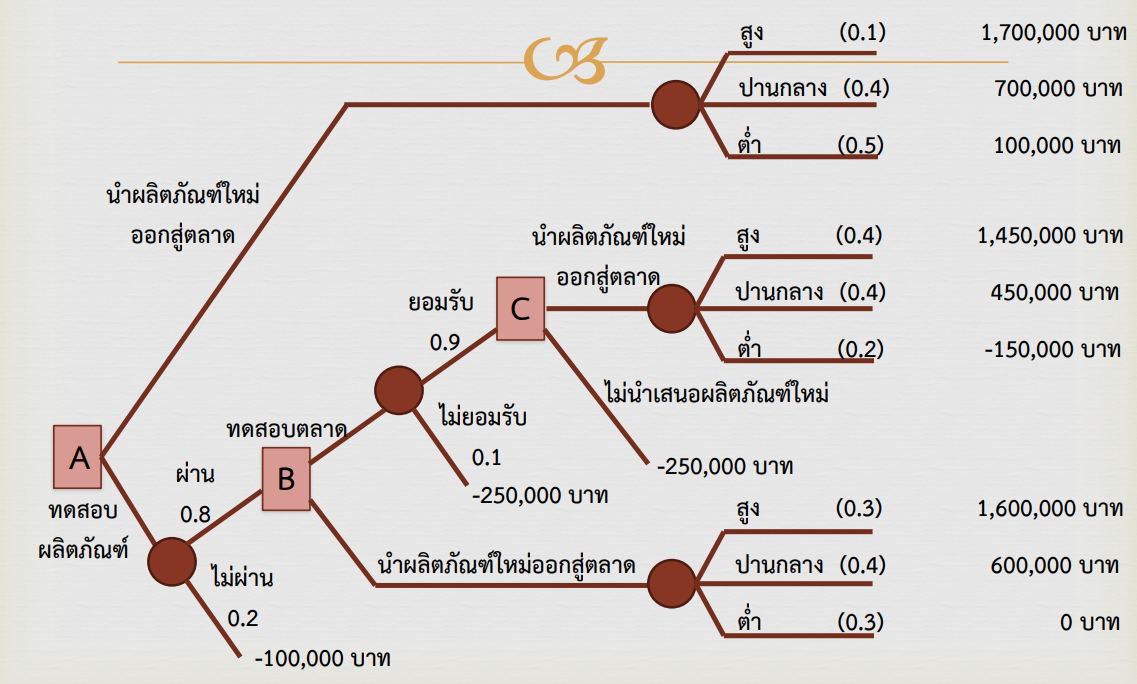
\includegraphics[width=1\linewidth]{solx.png}
\newpage
\section{การใช้โปรแกรม QM for Windows}
\newpage
\section*{Assignment (need revise)}
\subsection*{PART A:}
หลังจากบริษัท ABC Furniture ได้ใช้การวิเคราะห์เชิงเส้นในการวางแผนการผลิตช่วงไตรมาสก่อนหน้า  
บริษัทได้รับผลลัพธ์ที่ดีในช่วงแรก แต่ปัจจุบันกลับพบว่าไม่สามารถพึ่งพาแบบจำลองเดิมได้ตลอดเวลา  
เนื่องจากมีความไม่แน่นอนในตลาดสูงขึ้นเรื่อย ๆ เช่น ราคาวัตถุดิบผันผวน การแข่งขันสูง และความต้องการของลูกค้าที่แปรเปลี่ยนตลอด

\medskip
\noindent
\textbf{สถานการณ์ทางเลือก:} สำหรับไตรมาสถัดไป ฝ่ายผลิตเสนอ 3 กลยุทธ์ให้ฝ่ายบริหารพิจารณา:

\begin{itemize}
    \item \textbf{กลยุทธ์ A:} เพิ่มกำลังผลิต “โต๊ะทำงาน” ให้มากที่สุด โดยลดสัดส่วนตู้เก็บเอกสารลง
    \item \textbf{กลยุทธ์ B:} เพิ่มกำลังผลิต “ตู้เก็บเอกสาร” ให้มากที่สุด โดยลดสัดส่วนโต๊ะทำงานลง
    \item \textbf{กลยุทธ์ C:} กระจายการผลิตแบบสมดุลระหว่างทั้งสองประเภท
\end{itemize}

\noindent
\textbf{สถานการณ์ตลาด (States of Nature):}  
ฝ่ายการตลาดระบุว่าสถานการณ์ตลาดอาจเป็นไปได้ 3 แบบในไตรมาสหน้า:

\begin{itemize}
    \item \textbf{สถานการณ์ 1 (S1) — โต๊ะบูม:} โต๊ะทำงานขายดีมาก ตู้ขายได้น้อย
    \item \textbf{สถานการณ์ 2 (S2) — ตลาดสมดุล:} สินค้าทั้งสองขายได้ใกล้เคียงกัน
    \item \textbf{สถานการณ์ 3 (S3) — ตู้บูม:} ตู้เอกสารขายดีมาก โต๊ะขายได้น้อย
\end{itemize}

ฝ่ายบริหารต้องการทราบว่า ภายใต้แต่ละกลยุทธ์นั้น ถ้าเกิดสถานการณ์ตลาดแต่ละแบบ จะได้กำไรเท่าไร โดยฝ่ายวิเคราะห์ประเมินกำไร (หน่วย: พันบาท) ดังตาราง:

\begin{center}
\begin{tabular}{|c|c|c|c|}
\hline
\textbf{กลยุทธ์การผลิต} & \textbf{S1: โต๊ะบูม} & \textbf{S2: สมดุล} & \textbf{S3: ตู้บูม} \\
\hline
A (เน้นโต๊ะ) & 1,500 & 900 & 100 \\
B (เน้นตู้) & 200 & 800 & 1,400 \\
C (สมดุล) & 800 & 850 & 700 \\
\hline
\end{tabular}
\end{center}

\vspace{1em}
\noindent
\textbf{คำสั่ง:}

\begin{enumerate}
    % \item เขียนตารางผลตอบแทน (Payoff Table) จากข้อมูลข้างต้น (หากยังไม่ได้)
    \item วิเคราะห์การตัดสินใจภายใต้ความไม่แน่นอน โดยใช้เกณฑ์ต่อไปนี้:
    \begin{itemize}
        \item Maximax Criterion
        \item Maximin Criterion
        \item Laplace Criterion
        \item Hurwicz Criterion (ใช้ $\alpha = 0.6$)
        \item Minimax Regret Criterion
    \end{itemize}
    \item แต่ละเกณฑ์แนะนำกลยุทธ์ใด? อธิบายว่าแต่ละเกณฑ์สะท้อนทัศนคติความเสี่ยงแบบใด?
    \item ใช้โปรแกรม \textbf{QM for Windows} เพื่อคำนวณและตรวจสอบผลลัพธ์ พร้อมแนบภาพประกอบผลลัพธ์
\end{enumerate}

\subsection*{PART B:}
หลังจากฝ่ายบริหารบริษัท ABC Furniture ได้พิจารณาตารางผลตอบแทนจากกลยุทธ์ต่าง ๆ แล้ว  
ยังคงมีความลังเล เนื่องจากบริษัทไม่สามารถคาดการณ์สถานการณ์ตลาดล่วงหน้าได้อย่างแม่นยำ

คุณสมชายจึงเสนอแนวคิดว่า \emph{“หากบริษัทจ้างนักวิเคราะห์ตลาดมืออาชีพมาช่วยประเมินแนวโน้มตลาดก่อนได้หรือไม่?”}  
ซึ่งจะมีค่าใช้จ่ายในการจ้างทีมวิเคราะห์ภายนอกอยู่ที่ 150,000 บาท  
ทีมวิเคราะห์จะให้ผลลัพธ์เป็น \textbf{สัญญาณตลาดล่วงหน้า} (Market Signal) ซึ่งแบ่งเป็น 2 แบบคือ:

\begin{itemize}
    \item \textbf{สัญญาณบวก (Positive Signal):} แสดงว่าตลาดมีแนวโน้มดี
    \item \textbf{สัญญาณลบ (Negative Signal):} แสดงว่าตลาดมีแนวโน้มผันผวนหรือถดถอย
\end{itemize}

บริษัทสามารถเลือกที่จะ “เปิดกลยุทธ์ A, B หรือ C” หลังจากได้รับสัญญาณจากนักวิเคราะห์ก็ได้  
หรือจะตัดสินใจ “ไม่เปลี่ยนแผน” ก็ได้เช่นกัน

\medskip
\noindent
\textbf{ข้อมูลความแม่นยำของนักวิเคราะห์ตลาด} จากประวัติ:
\begin{itemize}
    \item หากสถานการณ์ตลาดเป็น \textbf{S1 (โต๊ะบูม)} $\rightarrow$ ให้สัญญาณบวก 80\%, สัญญาณลบ 20\%
    \item หากสถานการณ์ตลาดเป็น \textbf{S2 (สมดุล)} $\rightarrow$ ให้สัญญาณบวก 50\%, สัญญาณลบ 50\%
    \item หากสถานการณ์ตลาดเป็น \textbf{S3 (ตู้บูม)} $\rightarrow$ ให้สัญญาณบวก 30\%, สัญญาณลบ 70\%
\end{itemize}

\noindent
\textbf{ความน่าจะเป็นของแต่ละสถานการณ์ตลาด} (ตามฝ่ายการตลาดประเมิน):  
S1: 25\%, S2: 50\%, S3: 25\%

\medskip
\noindent
\textbf{คำสั่ง:}

\begin{enumerate}
    \item วาดแผนภาพ Decision Tree ที่เริ่มจากทางเลือก “จ้างนักวิเคราะห์” หรือ “ไม่จ้าง”
    \item แสดงการแตกเหตุการณ์ตามลำดับ: สัญญาณ → สถานการณ์ตลาด → กลยุทธ์การผลิต → ผลตอบแทนสุทธิ (หักค่าจ้าง)
    \item คำนวณ \textbf{Expected Monetary Value (EMV)} ของแต่ละทางเลือก (รวมต้นทุน 150,000 กรณีที่จ้าง)
    \item สร้างโมเดลนี้ใน \textbf{QM for Windows} เพื่อยืนยันผลลัพธ์ พร้อมแนบภาพผลลัพธ์
    \item คุณคิดว่าการจ้างนักวิเคราะห์มีความคุ้มค่าหรือไม่?
\end{enumerate}
	% !TEX root = ../BookTemplate.tex
%%%%%%%%%%%%%%%%%%%%%%%%%%%%%%%%%%%%%%%%%%%%%%%%%%%%%%%%%%%%%%%%%%%%%%%%%%%%%%%%%%
\chapter{ทฤษฎีการจำลองสถานการณ์ (Simulation)}

\section*{โจทย์ธุรกิจ: ความไม่แน่นอนในกระบวนการผลิตของ ABC Furniture}

\begin{tcolorbox}[colback=white!100!white, colframe=black!80!white,
  title=ข้อความจากคุณสมชาย,
  fonttitle=\bfseries,
  sharp corners=southwest,
  boxrule=0.8pt,
  left=1mm, right=1mm, top=1mm, bottom=1mm,
]
\emph{
"หลังจากที่เราได้วางแผนการผลิตและกลยุทธ์รับมือกับตลาดที่ไม่แน่นอนผ่านแบบจำลองเชิงเส้นและทฤษฎีการตัดสินใจเรียบร้อยแล้ว  
แต่สิ่งที่เรายังไม่สามารถคาดการณ์ได้แน่นอน คือเวลาที่ต้องใช้ในแต่ละขั้นตอนของกระบวนการผลิตจริง ๆ  
บางครั้งแรงงานลาป่วย บางครั้งเครื่องจักรเสีย หรือบางสัปดาห์มีคำสั่งซื้อเร่งด่วนแทรกเข้ามา  
เราจึงอยากจำลองสถานการณ์เหล่านี้ เพื่อดูว่าจะกระทบต่อการผลิตและการจัดส่งอย่างไร และควรจะปรับการจัดการโรงงานอย่างไรดี"
}
\end{tcolorbox}

บริษัท ABC Furniture กำลังเผชิญกับความไม่แน่นอนใน \textbf{ระยะเวลาการผลิตแต่ละชิ้นงาน} และ \textbf{ปริมาณคำสั่งซื้อที่เปลี่ยนแปลงตลอดเวลา} โดยเฉพาะในช่วงโปรโมชั่นและเทศกาลยอดนิยม ซึ่งอาจทำให้กระบวนการผลิตไม่สามารถดำเนินไปตามแผนได้

เพื่อรองรับเหตุการณ์ที่คาดเดาไม่ได้เหล่านี้ ผู้จัดการฝ่ายผลิตต้องการเครื่องมือในการ “ทดลอง” และ “คาดการณ์ผลลัพธ์” ของทางเลือกที่เป็นไปได้ โดยไม่ต้องเสี่ยงจริงในโลกธุรกิจจริง ซึ่งนำไปสู่แนวคิดของ \textbf{การจำลองสถานการณ์ (Simulation)} ที่จะช่วยให้บริษัทสามารถวิเคราะห์ผลกระทบจากตัวแปรสุ่มต่าง ๆ ต่อกระบวนการผลิตได้อย่างมีประสิทธิภาพ

\bigskip

\noindent\textbf{คำถามชวนคิด:}
\begin{itemize}
    \item ในสถานการณ์แบบนี้ คุณคิดว่า “สูตรคำนวณตายตัว” ที่เคยใช้ในบทก่อน ๆ ยังเหมาะสมอยู่หรือไม่?
    \item คุณจะเก็บข้อมูลอะไรเพื่อใช้ในการจำลองเหตุการณ์ในกระบวนการผลิต?
    \item คุณจะจำลองขั้นตอนใดในกระบวนการผลิตก่อน เช่น เวลาในการประกอบสินค้า การขนส่ง หรือการเตรียมวัตถุดิบ?
    \item ถ้าคุณลอง “สุ่มเหตุการณ์” ต่าง ๆ แล้วพบว่าเกิดความล่าช้าเป็นประจำ คุณจะวางแผนการผลิตใหม่อย่างไร?
    \item ถ้าต้องเขียนโปรแกรมจำลองขั้นตอนการผลิต คุณจะออกแบบลำดับเหตุการณ์หรือเงื่อนไขไว้อย่างไร?
    \item ผลลัพธ์ของการจำลองแบบใดที่จะช่วยให้ฝ่ายผลิตวางแผนจัดกำลังคนและเครื่องจักรได้ดีขึ้น?
\end{itemize}

\newpage
\section{แนวคิดเบื้องต้นของการจำลอง}
\begin{itemize}
    \item บางสถานการณ์อาจไม่สามารถเขียนสมการทางคณิตศาสตร์ตัวแบบเพื่ออธิบายสถานการณ์ได้เพราะระบบมีความซับซ้อนมากเกินไปหรือมีเงื่อนไขบางประการที่ทำให้ไม่สามารถใช้ตัวแบบที่มีอยู่แล้วได้
    \item ทำให้ต้องสุ่มภายใต้ข้อมูลที่มีเพื่อประมาณค่าจากการทำการทดลองสุ่มหลาย ๆ การทดลอง
    \item ในหัวข้อกรณีตัวอย่างที่จะกล่าวถึงถัดไป เป็นตัวอย่างพื้นฐานที่แสดงให้เห็นว่าการทำการทดลองสุ่มโดยที่จำลองสถานการณ์ให้เหมือน (หรือคล้าย) เหตุการณ์จริงจะสามารถประมาณค่าผลเฉลยให้ใกล้เคียงค่าจริงได้
\end{itemize}

\subsection{กรณีตัวอย่าง: การหาค่า $\pi$}
จากชุดความรู้เบื้องต้นที่เรามีคือ $\pi= \frac{\pi r^2}{r^2} = \frac{4\pi r^2}{(2r)^2} =4 \left( \frac{\text{พื้นที่วงกลม}}{\text{พื้นที่สี่เหลี่ยมจตุรัสที่แนบวงกลม}}\right)$
\begin{center}
\begin{tikzpicture}[scale=2]
  % Square
  \draw[thick] (-1,-1) rectangle (1,1);
  \node at (1.1,1.1) {$2r$};

  % Circle
  \draw[thick, fill=blue!10] (0,0) circle(1);
  \node at (0.6,0.2) {\small พื้นที่วงกลม = $\pi r^2$};

  % Square area label
  \node at (0,-1.3) {\small พื้นที่สี่เหลี่ยม = $(2r)^2 = 4r^2$};

  % Radius line
  \draw[->, thick, red] (0,0) -- (1,0) node[midway, below] {$r$};
\end{tikzpicture}
\end{center}
แต่เราไม่รู้ว่าค่า $\pi$ คือเท่าไหร่ เราจึงออกแบบการทดลองที่ถูกออกแบบให้อธิบายชุดความรู้ที่เรามีได้ ซึ่งก็คือการสุ่มโยนจุดเข้าไปในรูปสี่เหลี่ยม แล้วหาอัตราส่วนของจำนวนจุดที่อยู่ภายในวงกลม (แสดงถึงพื้นที่วงกลม) ต่อจำนวนจุดทั้งหมดที่โยนเข้าไป (แสดงถึงพื้นที่สี่เหลี่ยมจัตุรัส) แล้วนำอัตราส่วนที่ได้มาคูณกับ 4 จะได้ค่าประมาณของ $\pi$

เพื่อให้การสุ่มสามารถถูกควบคุมและวัดผลได้ เราจึงต้องใช้ระบบพิกัดฉากเข้ามาช่วยในการแสดงผล โดยที่เราจะให้จุดศูนย์กลางของวงกลมวางที่จุดกำเนิด และรัศมีของวงกลมมีค่าเท่ากับ $r=1$
\begin{center}
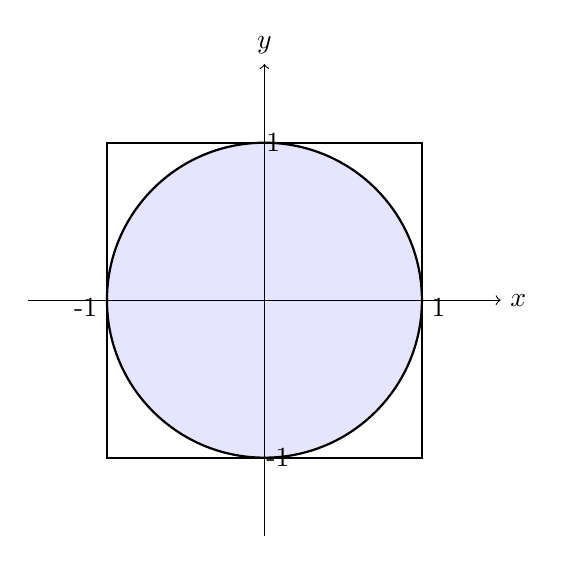
\begin{tikzpicture}[scale=2]
  % แกน x และ y
  % วงกลม
  \draw[thick, fill=blue!10] (0,0) circle(1);
  
  \draw[->] (-1.5,0) -- (1.5,0) node[right] {$x$};
  \draw[->] (0,-1.5) -- (0,1.5) node[above] {$y$};

  \draw (1,0.05) -- (1,-0.05) node[right] {1};
  \draw (-1,0.05) -- (-1,-0.05) node[left] {-1};
  \draw (0.05,1) -- (-0.05,1) node[right] {1};
  \draw (0.05,-1) -- (-0.05,-1) node[right] {-1};

  % สี่เหลี่ยมจัตุรัส
  \draw[thick] (-1,-1) rectangle (1,1);
\end{tikzpicture}
\end{center}
และเงื่อนไขการสุ่มจุด $(x,y)$ เป็นไปดังนี้
\begin{itemize}
    \item การสุ่มเป็นแบบ uniform กล่าวคือทุุกตำแหน่งมีโอกาสเท่ากัน
    \item สุ่ม $x$ และ $y$ อยู่ในช่วง $[-1,1]$ เพื่อให้มั่นใจว่าอยู่ภายในสี่เหลี่ยมจตุรัส
\end{itemize}
ทั้งนี้ การตรวจสอบว่าจุด $(x,y)$ อยู่ในวงกลมหรือไม่ เราสามารถเช็คได้ด้วยเงื่อนไขว่า
$$
x^2 + y^2 \leq 1
$$
ซึ่งเราสามารถใช้ Excel ช่วยในการสุ่มได้ดังนี้
\begin{itemize}
    \item Column A: ครั้งที่ทดลอง
    \item Column B-C: สุ่ม $x$ และ $y$ ด้วยคำสั่ง =RANDARRAY(จำนวนครั้งที่ทดลอง,2,-1,1,FALSE)
    \item Column D: เช็คว่าจุดอยู่ในวงกลมหรือไม่โดยใช้ ColumnB$\textasciicircum$2 + ColumnC$\textasciicircum$2 <= 1
    \item Column E: นับจำนวนจุดที่อยู่ในวงกลมตั้งแต่การทดลองที่ 1 จนถึงการทดลองปัจจุบัน
    \item Column F: หาค่า 4*อัตราส่วน
\end{itemize}
ตัวอย่าง 5 แถวแรกและ 5 แถวสุดท้ายของตารางกรณีสุ่ม 30000 ครั้ง:
\begin{center}
    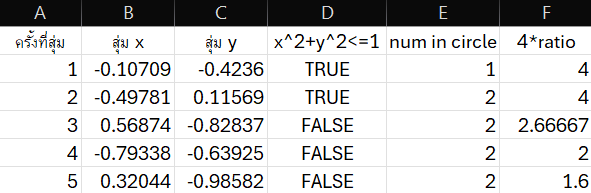
\includegraphics[width=0.7\linewidth]{image.png}
    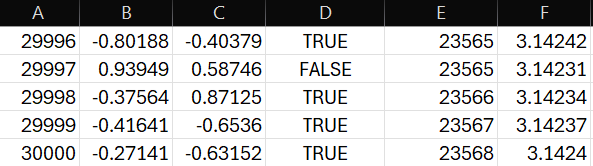
\includegraphics[width=0.7\linewidth]{image2.png}
\end{center}
และเมื่อลองทำการพล็อตกราฟของค่าที่เราสนใจ (Column F) จะได้ดังรูป
\begin{center}
    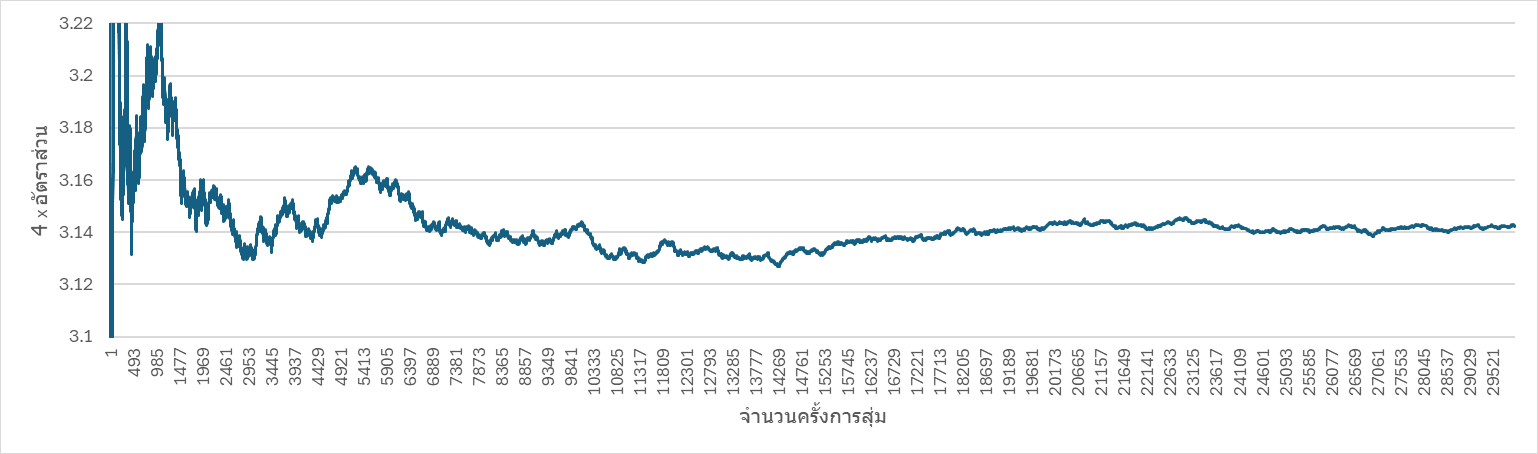
\includegraphics[width=\linewidth]{ratioToPi.png}
\end{center}
ซึ่งจะเห็นว่ายิ่งเราทำการสุ่มมากขึ้นเท่าไหร่ ค่าที่เราตั้งไว้ (4 เท่าของอัตราส่วน) เพื่อวัดสิ่งที่เราอยากค้นหา (ค่า $\pi$) จะยิ่งเข้าใกล้ค่าที่เราอยากค้นหาดังกล่าวมากขึ้นเรื่อยๆ

สามารถออกแบบการทดลองในทำนองเดียวกันคือทำการทดลองสุ่ม 30000 จุดหลาย ๆ รอบแล้วหาค่าเฉลี่ยค่าของรอบสุ่มที่ 30000 ของทุกชุดการทดลองก็ได้เช่นกันโดยรูปด้านล่างคือตัวอย่างการทดลองที่ทำการทดลอง 500 รอบ ซึ่งได้ค่าเฉลี่ยของค่าอัตราส่วนรอบที่ 30000 อยู่ที่ 3.141638 จากค่าประมาณจริง ๆ ของ $\pi\approx 3.1415926$ (ถ้าทำใน Excel อาจจะเจอปัญหาเรื่อง memory ไม่พอ แต่จะมีความแม่นยำกว่าการทดลองรอบเดียว เลยอาจต้องใช้เครื่องมือเช่นเขียน Python)
\begin{center}
    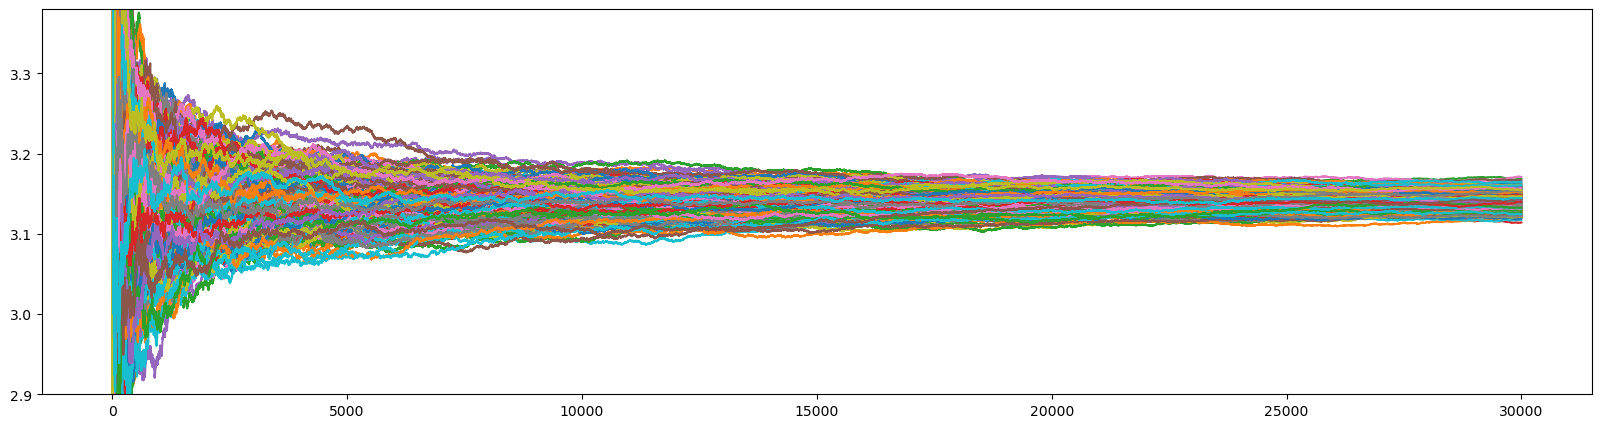
\includegraphics[width=1\linewidth]{SimulatePi.png}
\end{center}

ทั้งนี้ จะเห็นว่าเรามีการกำหนดเงื่อนไขการสุ่ม ซึ่งเป็นสิ่งที่สำคัญที่สุดของการจะจำลองสถานการณ์ ตัวอย่างเช่นกรณีนี้ก็คือต้องสุ่มแบบ Uniform เนื่องจากลักษณะการคำนวณอัตราส่วนของพื้นที่นั้นมีสมมติฐานว่าทุกจุดพื้นที่จะต้องมีความสำคัญเท่ากัน ไม่มีจุดใดจุดหนึ่งที่มีโอกาสมากกว่าจุดอื่นเพื่อไม่ให้เกิดอคติ (bias) ในการสุ่ม เช่นในตัวอย่างเดิม ถ้าเราเปลี่ยนสมมติฐานตั้งต้นให้สุ่มแบบ Normal Distribution ที่มีค่าเฉลี่ยเป็น 0 และส่วนเบี่ยงเบนมาตรฐานที่ 0.3 ที่จะมีโอกาสสุ่มได้บริเวณจุดกำเนิดมากกว่าจุดขอบ ๆ ซึ่งจะแสดงพฤติกรรมว่าจุดนอกวงกลมมีโอกาสน้อยกว่าจุดในวงกลม จะได้ว่าผลการประมาณค่าเปลี่ยนเป็น 3.9844 แทนที่จะเข้าใกล้ค่า $\pi$ ตามรูป
\begin{center}
    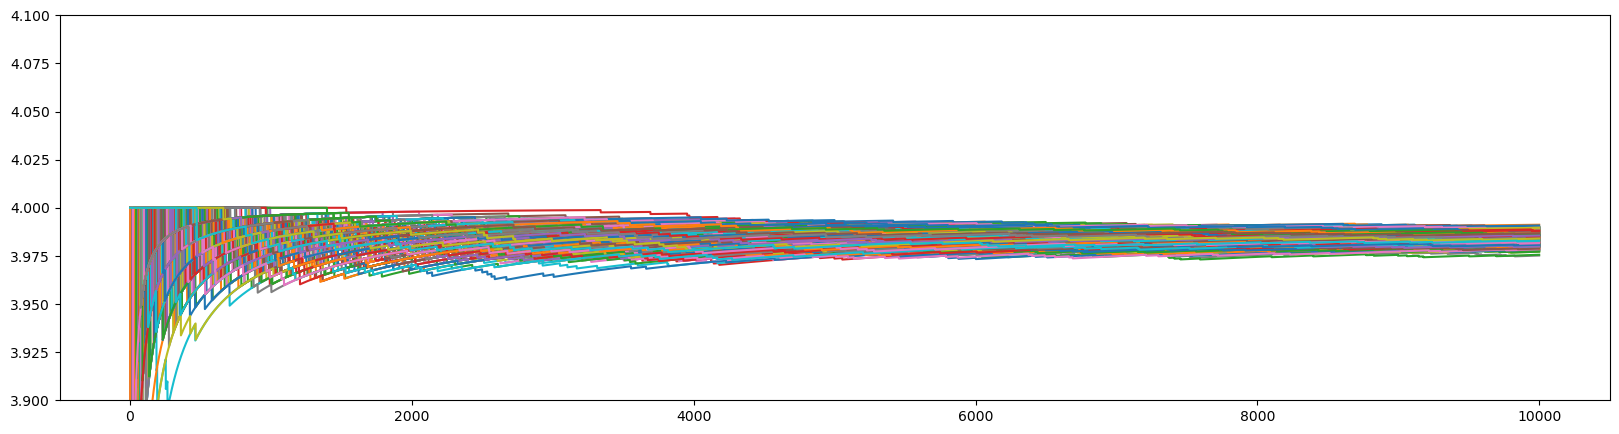
\includegraphics[width=1\linewidth]{simulatePiWrong.png}
\end{center}

\begin{tcolorbox}[colback=white!100!white, colframe=black!80!white,
  title=หมายเหตุ (สำหรับอ่านเพิ่มเติม),
  fonttitle=\bfseries,
  sharp corners=southwest,
  boxrule=0.8pt,
  left=1mm, right=1mm, top=1mm, bottom=1mm, breakable
]
    ตัวอย่างนี้เป็นตัวอย่างที่มีทฤษฎีเบื้องหลังและสามารถพิสูจน์ทางคณิตศาสตร์เพื่อยืนยันว่าผลที่ได้จากการทดลองเป็นไปตามทฤษฎี (อาจมีคลาดเคลื่อนเล็กน้อย) เนื่องจากเป็นสถานการณ์ที่สามารถอธิบายได้ด้วยการแจกแจงความน่าจะเป็นที่ไม่ซับซ้อน (ซึ่งไม่ค่อยพบในโลกจริงที่มักจะเป็นระบบที่ซับซ้อน)
    \newpage
    \textbf{กรณีที่ $X, Y$ แจกแจงแบบคงที่}
    \begin{proof}
        กำหนดให้ $X, Y$ เป็นตัวแปรสุ่มอิสระ ซึ่งแจกแจงแบบสม่ำเสมอ (Uniform) บนช่วง $[-1, 1]$ ดังนั้นคู่ $(X, Y)$ จะกระจายอยู่ทั่วพื้นที่ของสี่เหลี่ยมจัตุรัสที่มีด้านยาว 2 หน่วย และมีพื้นที่รวมเท่ากับ $4$ หน่วยตาราง

        นิยามเหตุการณ์ $A$ ว่าเป็นเหตุการณ์ที่จุด $(X, Y)$ ตกอยู่ภายในวงกลมรัศมี 1 ซึ่งมีสมการคือ $X^2 + Y^2 \leq 1$

        จะได้ว่า
        \[
            P((X, Y) \in A) = \frac{\text{พื้นที่ของวงกลม}}{\text{พื้นที่ของสี่เหลี่ยมจัตุรัส}} = \frac{\pi \cdot 1^2}{4} = \frac{\pi}{4}
        \]

        เมื่อสุ่มจุด $N$ จุดจากการแจกแจงนี้ ให้ $S$ เป็นจำนวนจุดที่ตกในวงกลม จะได้ว่า $S = \sum_{i=1}^N \mathbf{1}_{(X_i, Y_i) \in A}$

        ดังนั้นสัดส่วนของจุดที่อยู่ในวงกลมคือ $Z = \frac{S}{N}$ ซึ่งเป็นตัวแปรสุ่ม และค่าคาดหมายคือ:
        \[
            \mathbb{E}\left[Z\right] =\mathbb{E}\left[\frac{S}{N}\right] = \frac{1}{N} \sum_{i=1}^N \mathbb{E}\left[\mathbf{1}_{(X_i, Y_i) \in A}\right] = P((X, Y) \in A) = \frac{\pi}{4}
        \]

        นั่นคือ ค่าคาดหวังของสัดส่วนของจุดที่อยู่ในวงกลมจะมีค่าเท่ากับ $\frac{\pi}{4}$ เสมอ โดยไม่ขึ้นกับจำนวนจุด $N$
    \end{proof}
    \vspace{1em}

    \textbf{กรณีที่ $X, Y \sim \mathcal{N}(0, 0.09)$} (ค่าความเบี่ยงเบนมาตรฐาน $\sigma = 0.3$)
    \begin{proof}
        เนื่องจากบทพิสูจน์ในส่วนของตัวแปรสุ่ม $Z$ ไม่ขึ้นกับการแจกแจงของตัวแปรสุ่ม $X,Y$ ดังนั้น เราจึงยังสามารถได้ผลว่า
        \[
            \mathbb{E}\left[Z\right] =\mathbb{E}\left[\frac{S}{N}\right] = P((X, Y) \in A)
        \]
        เหลือแค่หาค่าความน่าจะเป็น $P((X, Y) \in A) = P(X^2 + Y^2 \leq 1)$ พิจารณาตัวแปรสุ่ม $R^2=X^2 + Y^2$ ซึ่งจากนิยามของการแจกแจง Chi-square (ผลรวมกำลังสองของตัวแปรสุ่มที่มีการแจกแจงปกติมาตรฐาน) จะได้ว่า
        $$
        \frac{R^2}{0.09}=\frac{X^2 + Y^2}{\sigma^2} = \left( \frac{X}{\sigma} \right)^2 + \left( \frac{Y}{\sigma} \right)^2 \sim \chi^2(2)
        $$
        ดังนั้น $P(R^2 \leq 1) = P(\chi^2(2) \leq \frac{1}{0.09}) = 1-\exp{-\frac{1}{2\times 0.09}}$\\
        เพราะฉะนั้น $E[4Z] = 4P(R^2\leq 1) = 4\left( 1-\exp{-\frac{1}{2\times 0.09}}\right)\approx 3.9845$
    \end{proof}
\end{tcolorbox}


\newpage
\section{ตัวแบบและขั้นตอนการจำลองสถานการณ์ (Simulation Process)}

จากตัวอย่างที่แล้ว เราได้เห็นกระบวนการที่สำคัญของการจำลองสถานการณ์ (Simulation) ซึ่งประกอบไปด้วยขั้นตอนหลัก ๆ ตั้งแต่การกำหนดวัตถุประสงค์, การเก็บข้อมูล, การเลือกตัวแบบ, การสุ่มตัวอย่าง และการวิเคราะห์ผลลัพธ์ที่ได้จากการทดลอง ในหัวข้อนี้เราจะสรุปขั้นตอนที่จำเป็นทั้งหมดในการจำลองสถานการณ์ทั่วไป ซึ่งสามารถนำไปประยุกต์ใช้กับสถานการณ์ทางธุรกิจต่าง ๆ ได้อย่างเป็นระบบ

กระบวนการในการจำลองสถานการณ์ประกอบด้วยขั้นตอนที่สำคัญ ดังนี้:

\begin{enumerate}
    \item \textbf{กำหนดวัตถุประสงค์ของการจำลอง (Define Simulation Objective)}\\
    ขั้นตอนแรกคือการระบุให้ชัดเจนว่าการจำลองครั้งนี้มีเป้าหมายอะไร เช่น บริษัท ABC Furniture ต้องการจำลองระยะเวลาในการผลิตสินค้าเพื่อดูว่าจะส่งผลต่อการส่งมอบสินค้าได้ทันตามกำหนดหรือไม่
    
    \item \textbf{กำหนดตัวแบบและตัวแปรที่เกี่ยวข้อง (Identify the Model and Relevant Variables)}\\
    หลังจากรู้วัตถุประสงค์แล้ว เราต้องกำหนดว่าอะไรคือสิ่งที่เราจะจำลอง ในทางธุรกิจอาจมีตัวแปรเช่น เวลามาถึงของลูกค้า, ระยะเวลาการผลิตสินค้า, ระยะเวลาการให้บริการ, หรือแม้กระทั่งปริมาณความต้องการของตลาดในแต่ละช่วงเวลา เป็นต้น
    
    \item \textbf{เก็บรวบรวมข้อมูลจากระบบจริง (Data Collection)}\\
    เมื่อระบุตัวแปรที่เกี่ยวข้องแล้ว ขั้นตอนถัดไปคือการเก็บข้อมูลเพื่อระบุลักษณะทางสถิติของตัวแปรนั้น ๆ เช่น การเก็บข้อมูลเวลาการผลิตจริงย้อนหลังหลายสัปดาห์ หรือข้อมูลพฤติกรรมของลูกค้าที่เกิดขึ้นจริงในอดีต
    
    \item \textbf{เลือกและสร้างแบบจำลองความน่าจะเป็น (Select and Build Probability Models)}\\
    หลังจากเก็บข้อมูล เราจึงนำข้อมูลนั้นมาวิเคราะห์เพื่อระบุการแจกแจงความน่าจะเป็นที่เหมาะสม เช่น เวลาการผลิตอาจเป็นแบบ Normal หรือ Exponential, จำนวนลูกค้าที่เข้าร้านอาจมีการแจกแจงแบบ Poisson หรือแบบ Uniform ดังในตัวอย่างที่ผ่านมาที่เราใช้ Uniform ในการประมาณค่า $\pi$
    
    \item \textbf{กำหนดเงื่อนไขการสุ่มและกฎของระบบ (Define Randomness Conditions and System Rules)}\\
    ขั้นตอนนี้คือการออกแบบกลไกของการจำลอง เช่น จะสุ่มตัวแปรต่าง ๆ อย่างไร ต้องใช้เครื่องมืออะไร มีเงื่อนไขและข้อจำกัดของระบบอย่างไรบ้าง เช่น บริษัท ABC Furniture อาจตั้งเงื่อนไขว่าหากการผลิตล่าช้ากว่าเวลาที่กำหนด จะส่งผลต่อกำหนดการจัดส่งสินค้าอย่างไร เป็นต้น
    
    \item \textbf{ดำเนินการจำลองสถานการณ์ (Perform Simulation Runs)}\\
    เมื่อโมเดลพร้อมแล้ว จะต้องดำเนินการจำลองซ้ำหลายครั้ง (replications) เพื่อให้ได้ผลลัพธ์ที่สะท้อนพฤติกรรมระบบจริงอย่างถูกต้องชัดเจน โดยอาจดำเนินการซ้ำหลายร้อยหรือหลายพันครั้งขึ้นอยู่กับลักษณะของปัญหา
    
    \item \textbf{วิเคราะห์ผลลัพธ์ที่ได้จากการจำลอง (Analyze Simulation Results)}\\
    หลังจากที่ทำการทดลองจำลองซ้ำหลาย ๆ รอบแล้ว เราจะนำผลลัพธ์ที่ได้มาวิเคราะห์เชิงสถิติ เช่น การหาค่าเฉลี่ย, ส่วนเบี่ยงเบนมาตรฐาน, ความน่าจะเป็นของเหตุการณ์ที่สนใจ เช่น โอกาสที่สินค้าไม่สามารถส่งมอบทันเวลา หรือเวลารอคอยเฉลี่ยของลูกค้า เป็นต้น
    
    \item \textbf{ตรวจสอบความถูกต้องและความแม่นยำของตัวแบบ (Validate and Verify the Model)}\\
    ก่อนนำไปใช้งานจริง เราต้องตรวจสอบว่าผลลัพธ์จากแบบจำลองนั้นตรงกับสิ่งที่เกิดขึ้นในระบบจริงมากแค่ไหน หากผลที่ได้จากตัวแบบมีความคลาดเคลื่อนสูง เราต้องกลับไปตรวจสอบข้อมูลหรือโมเดลที่ใช้ใหม่
    
    \item \textbf{การนำผลลัพธ์ไปประยุกต์ใช้ในทางปฏิบัติ (Implementation and Decision Making)}\\
    ขั้นตอนสุดท้ายคือการนำผลที่ได้จาก Simulation ไปใช้ในการตัดสินใจจริงในธุรกิจ เช่น บริษัท ABC Furniture อาจนำผลการจำลองไปกำหนดแผนการผลิตและจัดการทรัพยากรใหม่เพื่อลดความเสี่ยงในการผลิตและเพิ่มประสิทธิภาพของระบบ
\end{enumerate}

กระบวนการทั้งหมดนี้สามารถสรุปออกมาในลักษณะของแผนภาพดังนี้

\begin{center}
    \begin{tikzpicture}[node distance=1.5cm,auto,font=\small]
        \node[draw, rounded corners, fill=blue!10] (start) {กำหนดวัตถุประสงค์};
        \node[draw, rounded corners, fill=blue!10, below of=start] (identify) {กำหนดตัวแปรที่เกี่ยวข้อง};
        \node[draw, rounded corners, fill=blue!10, below of=identify] (collect) {เก็บข้อมูลจากระบบจริง};
        \node[draw, rounded corners, fill=blue!10, below of=collect] (prob) {เลือกและสร้างแบบจำลองความน่าจะเป็น};
        \node[draw, rounded corners, fill=blue!10, below of=prob] (rules) {กำหนดเงื่อนไขการสุ่มและกฎของระบบ};
        \node[draw, rounded corners, fill=blue!10, below of=rules] (simu) {ดำเนินการจำลอง};
        \node[draw, rounded corners, fill=blue!10, below of=simu] (analyze) {วิเคราะห์ผลลัพธ์};
        \node[draw, rounded corners, fill=blue!10, below of=analyze] (validate) {ตรวจสอบความถูกต้อง};
        \node[draw, rounded corners, fill=blue!10, below of=validate] (implement) {นำไปใช้ในการตัดสินใจ};

        \draw[->, thick] (start) -- (identify);
        \draw[->, thick] (identify) -- (collect);
        \draw[->, thick] (collect) -- (prob);
        \draw[->, thick] (prob) -- (rules);
        \draw[->, thick] (rules) -- (simu);
        \draw[->, thick] (simu) -- (analyze);
        \draw[->, thick] (analyze) -- (validate);
        \draw[->, thick] (validate) -- (implement);
    \end{tikzpicture}
\end{center}

โดยในหัวข้อถัดไป เราจะศึกษาและเจาะลึกเทคนิคการสุ่มแบบ Monte Carlo ซึ่งเป็นหัวใจสำคัญของกระบวนการจำลองสถานการณ์ในธุรกิจ เพื่อให้เห็นภาพการประยุกต์ใช้กระบวนการจำลองได้อย่างเป็นระบบยิ่งขึ้น

\section{การสุ่มตัวอย่างแบบ Monte Carlo ในการจำลองสถานการณ์ในธุรกิจ}
\textbf{การจำลองแบบมอนติคาร์โล} (Monte Carlo Simulation) เป็นเทคนิคที่ใช้วิธีการสุ่มตัวแปรเข้ามาช่วยในการประเมินผลลัพธ์ที่อาจเกิดขึ้นภายใต้สภาวะที่ไม่แน่นอน เทคนิคนี้มีรากฐานจากแนวคิดในทฤษฎีความน่าจะเป็นและสถิติ โดยเฉพาะอย่างยิ่งเมื่อปัญหาที่ต้องการศึกษามีความซับซ้อนเกินกว่าจะหาคำตอบได้ด้วยวิธีวิเคราะห์เชิงพีชคณิตแบบตรง

แก่นของมอนติคาร์โลคือการ “สุ่มค่าตัวแปรตามการแจกแจงที่กำหนด” เพื่อนำไปแทนค่าในโมเดล แล้วคำนวณผลลัพธ์ที่เกิดขึ้น จากนั้นทำซ้ำการสุ่มจำนวนมากเพื่อดูพฤติกรรมรวมของผลลัพธ์ เช่น ค่าคาดหมาย ค่ามากสุด ค่าน้อยสุด หรือค่าที่อยู่ในช่วงความเชื่อมั่นที่กำหนด โดยตัวอย่างการแจกแจงที่นิยมใช้งานกันอยู่แล้วมีดังนี้
\begin{itemize}
    \item ถ้าค่าใช้จ่ายในอนาคตมีความไม่แน่นอน อาจสุ่มค่าใช้จ่ายจากการแจกแจง Normal หรือ Triangular
    \item ถ้าความต้องการสินค้าในอนาคตขึ้นอยู่กับพฤติกรรมผู้บริโภค อาจสุ่มจำนวนจากการแจกแจง Poisson
    \item ถ้าความสำเร็จของกระบวนการหรือขั้นตอนมีแค่ 2 ผลลัพธ์ (สำเร็จ/ล้มเหลว ในภาษาของการแจกแจงความน่าจะเป็น) อาจใช้การแจกแจงแบบ Bernoulli หรือ Binomial
    \item ถ้าจำนวนลูกค้าในช่วงเวลาหนึ่งมีความแปรผัน อาจใช้การแจกแจง Poisson เพื่อสุ่มจำนวนลูกค้า
    \item ถ้าเวลาระหว่างลูกค้ารายถัดไปมีลักษณะสุ่มและต่อเนื่อง อาจใช้การแจกแจง Exponential เพื่อสุ่มระยะเวลาการรอลูกค้าเข้าร้าน
\end{itemize}
ซึ่งเป็นขั้นตอนที่สำคัญมาก ๆ และการเก็บข้อมูลและลายละเอียดพฤติกรรมทางธุรกิจให้ละเอียดพอจะช่วยทำให้เราเลือกการแจกแจงของตัวแปรได้แม่นยำและใกล้เคียงความเป็นจริงได้ (อาจจะใช้เรื่องการทำ goodness of fit test มาช่วยตรวจสอบในขั้นตอนการตรวจสอบได้)

\subsection*{5 ขั้นตอนการทำ Monte Carol Simulation}
\begin{enumerate}
    \item \textbf{กำหนดการแจกแจงความน่าจะเป็นของตัวแปรสำคัญ} \\
    ระบุ \textit{ตัวแปรสำคัญ} ที่ต้องการจำลอง เช่น ความต้องการสินค้า เวลารอ จำนวนลูกค้าในแต่ละวัน ฯลฯ จากนั้นคำนวณ \textit{ความน่าจะเป็น} โดยใช้ข้อมูลในอดีต เช่น ความถี่ของแต่ละเหตุการณ์หารด้วยความถี่รวมทั้งหมด
    
    \item \textbf{สร้างการแจกแจงความน่าจะเป็นสะสม (Cumulative Probability)} \\
    สร้างคอลัมน์ความน่าจะเป็นสะสม โดยการบวกค่าความน่าจะเป็นในข้อก่อนหน้าแบบสะสมต่อเนื่อง เพื่อใช้เป็นขอบเขตในการแมปกับช่วงของเลขสุ่ม
    
    \item \textbf{กำหนดช่วงของเลขสุ่ม (Random Number Interval)} \\
    แปลงความน่าจะเป็นสะสมให้เป็นช่วงของเลขสุ่ม เช่น 00--99 หรือ 000--999 โดยการจับคู่ค่าที่เป็นไปได้กับช่วงของตัวเลข เช่น ความน่าจะเป็น 0.2 อาจแทนด้วยเลขสุ่ม 00--19
    
    \item \textbf{สร้างเลขสุ่ม (Generate Random Numbers)} \\
    สร้างเลขสุ่มจำนวนหนึ่งโดยใช้เครื่องมือ เช่น ตารางเลขสุ่ม Excel หรือโปรแกรมคอมพิวเตอร์ เพื่อสุ่มค่าที่จะนำไปใช้ในการทดลองจำลองแต่ละรอบ
    
    \item \textbf{จำลองการทดลองหลายรอบ (Simulate a Series of Trials)} \\
    ทำการจำลองสถานการณ์โดยใช้เลขสุ่มในแต่ละรอบ เพื่อระบุค่าที่เกิดขึ้น แล้วนำข้อมูลที่ได้จากการทดลองไปวิเคราะห์ เช่น หาค่าเฉลี่ย ความแปรปรวน หรือพฤติกรรมของระบบในระยะยาว
\end{enumerate}

\begin{example}
    {การจำลองความต้องการยางรถยนต์}{}
    บริษัท ไทยไทร์ จำกัด เป็นผู้จัดจำหน่ายยางรถยนต์หลายประเภทในประเทศไทย โดยมียางรถยนต์รุ่นยอดนิยมรุ่นหนึ่งที่มียอดขายสูงเป็นพิเศษ  
    ฝ่ายคลังสินค้าสังเกตว่าต้นทุนจากการเก็บรักษาสินค้าคงคลัง (Inventory Cost) ของยางรุ่นนี้เริ่มสูงขึ้น และต้องการนโยบายการบริหารจัดการสินค้าคงคลังที่เหมาะสม  
    เพื่อดูแนวโน้มความต้องการยางในแต่ละวัน ผู้จัดการจึงตัดสินใจใช้การจำลองสถานการณ์ (Simulation) เพื่อดูความต้องการรายวันเป็นเวลา 10 วัน 
    \begin{enumerate}
        \item จงหาค่าความต้องการยางเฉลี่ยต่อวัน (จากการแจกแจงความน่าจะเป็นดั้งเดิม)
        \item จงหาค่าความต้องการยางเฉลี่ยต่อวันจากการจำลองสถานการณ์
    \end{enumerate}
\end{example}
\begin{tabular}{|c|c|}
    \hline
    \textbf{จำนวนที่ต้องการต่อวัน (เส้น)} & \textbf{ความถี่ (วัน)} \\
    \hline
    0 & 10 \\
    1 & 20 \\
    2 & 40 \\
    3 & 60 \\
    4 & 40 \\
    5 & 30 \\
    \hline
    \textbf{รวม} & \textbf{200} \\
    \hline
\end{tabular}
\newpage
\begin{example}
    {Inventory Analysis Usecase}{}
    คุณภูวเดชเป็นเจ้าของร้านเครื่องมือช่างชื่อ \textbf{เจริญวัสดุภัณฑ์} ซึ่งจำหน่ายเครื่องมือช่างหลากหลายประเภท และสินค้าที่ขายดีและทำกำไรสูงคือ \textbf{สว่านไฟฟ้ารุ่น Ace} คุณภูวเดชต้องการหานโยบายการจัดเก็บสินค้าคงคลังที่ต้นทุนต่ำที่สุดสำหรับสินค้ารุ่นนี้ แต่เนื่องจากว่าไม่สามารถควบคุมปัจจัยภายนอกบางประการได้ จึงตัดสินใจใช้วิธีการ \textbf{การจำลองสถานการณ์ (Simulation)} เพื่อช่วยในการตัดสินใจ

ในปัญหานี้ ตัวแปรที่ควบคุมได้ (Controllable Inputs) คือ
\begin{itemize}
    \item \textbf{จำนวนที่สั่งแต่ละครั้ง (Order Quantity)} และ 
    \item \textbf{จุดสั่งซื้อใหม่ (Reorder Point)}
\end{itemize}
ส่วนตัวแปรที่ควบคุมไม่ได้ (Uncontrollable Inputs) คือ
\begin{itemize}
    \item \textbf{ความต้องการต่อวัน (Daily Demand)} ซึ่งมีความผันแปร
    \item \textbf{ระยะเวลาในการจัดส่ง (Lead Time)} ซึ่งมีความไม่แน่นอนเช่นกัน
\end{itemize}

\textbf{คุณภูวเดชได้เก็บข้อมูลยอดขายจริงของสว่านรุ่น Ace ตลอด 300 วัน} โดยสรุปไว้ในตารางดังนี้:

\begin{center}
\begin{tabular}{|c|c|}
\hline
\textbf{ความต้องการต่อวัน (ตัว)} & \textbf{ความถี่ (วัน)} \\
\hline
0 & 15 \\
1 & 30 \\
2 & 60 \\
3 & 120 \\
4 & 45 \\
5 & 30 \\
\hline
\textbf{รวม} & \textbf{300} \\
\hline
\end{tabular}
\end{center}

เมื่อมีการสั่งซื้อสินค้า จะต้องรอสินค้าจัดส่งภายใน 1 ถึง 3 วัน โดยมีข้อมูลสรุปจากคำสั่งซื้อ 50 รายการที่ผ่านมาตามตารางต่อไปนี้:

\begin{center}
\begin{tabular}{|c|c|}
\hline
\textbf{ระยะเวลาในการส่งสินค้า (วัน)} & \textbf{ความถี่ (ครั้ง)} \\
\hline
1 & 10 \\
2 & 25 \\
3 & 15 \\
\hline
\textbf{รวม} & \textbf{50} \\
\hline
\end{tabular}
\end{center}

คุณภูวเดชต้องการทดลองใช้นโยบาย \textbf{สั่งซื้อเมื่อสินค้าคงเหลือน้อยกว่าหรือเท่ากับ 5 ชิ้น โดยสั่งครั้งละ 10 ชิ้น} และกำหนดให้ในวันแรกมีสินค้าในสต็อก 10 ชิ้น
\newpage
\textbf{ข้อมูลต้นทุนประกอบด้วย:}
\begin{itemize}
    \item ค่าดำเนินการสั่งซื้อสินค้าแต่ละครั้ง = 10 บาท
    \item ค่าถือครองสินค้าต่อปี = 6 บาทต่อชิ้น หรือเท่ากับ 0.03 บาทต่อชิ้นต่อวัน (คิดจากปีละ 200 วัน)
    \item ค่าขาดแคลนสินค้าหรือลูกค้าไม่ได้สินค้า = 8 บาทต่อครั้ง
\end{itemize}

\textbf{กำหนดให้ร้านเปิดบริการ 200 วันต่อปี และใช้ตัวเลขสุ่มต่อไปนี้ในการทดลอง:}\\
\texttt{06 63 57 94 52 69 32 30 48 88}

\vspace{1em}
\textbf{คำถาม}
\begin{enumerate}[label=\alph*)]
    \item จงคำนวณ \textbf{ตารางแจกแจงความน่าจะเป็น, ความน่าจะเป็นสะสม และช่วงตัวเลขสุ่ม (Random Number Interval)} สำหรับทั้งสองตาราง
    \item จากนโยบายการสั่งซื้อที่กำหนดไว้ ($Q = 10$, $ROP = 5$) จงคำนวณ \textbf{ต้นทุนเฉลี่ยต่อวัน} ของร้านในช่วง 10 วันแรก จากการจำลองสถานการณ์

    \textit{คำใบ้: ต้นทุนรวมต่อวัน = ค่าสั่งซื้อเฉลี่ยต่อวัน + ค่าถือครองเฉลี่ยต่อวัน + ค่าขาดแคลนเฉลี่ยต่อวัน}
\end{enumerate}
\end{example}
\newpage
\section*{Assignment}

...
	\chapter{การวิเคราะห์เชิงมาร์คอฟ (Markov Analysis)}

\section*{โจทย์ธุรกิจ}
\textbf{สถานการณ์ต้นบท: ความภักดีของลูกค้า (Customer Loyalty)}

หลังจากผ่านสถานการณ์ความไม่แน่นอนของตลาดและการตัดสินใจเรื่องกลยุทธ์การผลิตแล้ว  
ฝ่ายการตลาดของบริษัท ABC Furniture สังเกตเห็นปรากฏการณ์สำคัญที่กำลังส่งผลต่อผลประกอบการของบริษัท นั่นคือเรื่องของ \textbf{“การรักษาฐานลูกค้าจากบริการหลังการขาย”}

คุณสมชายและฝ่ายการตลาดพบข้อมูลที่น่าสนใจว่า ในแต่ละไตรมาส ลูกค้าของบริษัทมีแนวโน้มที่จะเปลี่ยนแปลงพฤติกรรมในการใช้บริการหลังการขายดังนี้:

\begin{itemize}
    \item ลูกค้าบางส่วนเป็น \textbf{ลูกค้าประจำ (Loyal Customers)} ที่ใช้บริการต่อเนื่องทุกไตรมาส
    \item ลูกค้าบางส่วนเป็น \textbf{ลูกค้าเปลี่ยนใจง่าย (Occasional Customers)} ที่ใช้บริการบ้างไม่ใช้บริการบ้าง
    \item ลูกค้าบางส่วนเป็น \textbf{ลูกค้าที่หายไป (Lost Customers)} ซึ่งหยุดใช้บริการจากบริษัท
\end{itemize}

ฝ่ายการตลาดต้องการวิเคราะห์ว่า ในแต่ละไตรมาสนั้น ลูกค้าจะเปลี่ยนแปลงสถานะจากกลุ่มหนึ่งไปอีกกลุ่มหนึ่งอย่างไร  
เพื่อที่จะได้วางแผนกลยุทธ์การตลาดและการบริหารความสัมพันธ์กับลูกค้า (CRM) ให้เหมาะสม

\vspace{0.5em}
\noindent
\textbf{อีเมลจากคุณสมชาย:}
\begin{tcolorbox}[colback=white!100!white, colframe=black!80!white,
  title=ข้อความ,
  fonttitle=\bfseries,
  sharp corners=southwest,
  boxrule=0.8pt,
  left=1mm, right=1mm, top=1mm, bottom=1mm,
]
\emph{
``ในช่วงไตรมาสที่ผ่านมา เราเริ่มสังเกตเห็นว่าฐานลูกค้าของเราเปลี่ยนแปลงเร็วมาก  
มีลูกค้าประจำหลายรายที่กลายเป็นลูกค้าเปลี่ยนใจง่าย  
และลูกค้ากลุ่มเปลี่ยนใจง่ายจำนวนไม่น้อยที่หยุดใช้บริการเราไปเลย  
แต่ในทางกลับกัน ก็ยังมีลูกค้าใหม่ๆ ที่เปลี่ยนจากลูกค้าเปลี่ยนใจง่ายมาเป็นลูกค้าประจำได้ด้วย  
เราอยากวิเคราะห์ให้ลึกกว่านี้ว่าการเปลี่ยนสถานะของลูกค้าเกิดขึ้นในลักษณะไหน  
เพื่อช่วยให้เราออกแบบกลยุทธ์รักษาฐานลูกค้าได้ดีขึ้นครับ"}
\end{tcolorbox}

\vspace{1em}
\noindent
\textbf{คำถามชวนคิดก่อนเรียน:}
\begin{enumerate}
    \item จากสถานการณ์ที่คุณสมชายเล่าให้ฟัง บริษัท ABC Furniture กำลังเจอกับปัญหาลักษณะใด?
    \item คุณคิดว่าการเปลี่ยนแปลงพฤติกรรมของลูกค้าในแต่ละไตรมาสเป็นเรื่องที่วิเคราะห์ได้อย่างไร?
    \item หากคุณจะสร้างแบบจำลองเพื่อวิเคราะห์พฤติกรรมลูกค้า คุณควรเก็บข้อมูลลักษณะใดบ้าง?
    \item สถานการณ์เช่นนี้ เหตุใดบริษัทจึงควรสนใจเรื่อง “การรักษาฐานลูกค้า” มากกว่าการหาลูกค้าใหม่เพียงอย่างเดียว?
    \item คุณคิดว่าการเปลี่ยนจากลูกค้าประจำไปเป็นลูกค้าเปลี่ยนใจง่าย หรือไปเป็นลูกค้าหายไป มีความสำคัญต่างกันหรือไม่ อย่างไร?
\end{enumerate}

\newpage
\section{ลักษณะของปัญหาที่ใช้ตัวแบบมาร์คอฟแก้ปัญหา}
\begin{itemize}
    \item ตัวแบบมาร์คอฟจะพิจารณาถึงความไม่แน่นอนของการเปลี่ยนสถานะในอนาคตโดยอ้างอิงจากสถานะในปัจจุบัน
    \item เพราะฉะนั้นปัญหาที่จะใช้ตัวแบบมาร์คอฟต้องสามารถแจกจางสถานะ (state) ขาดออกจากกันได้ โดยแต่ละตัวอย่างจะต้องอยู่ในสถานะใดสถานะหนึ่งและเพียงสถานะเดียวเท่านั้น
    \item ต้องมีข้อมูลเกี่ยวกับการแจกแจงความน่าจะเป็นหรืออัตราส่วนของแต่ละสถานะในปัจจุบัน
    \item ต้องทราบข้อมูลเรื่องความน่าจะเป็นของการเปลี่ยนสถานะ (transition probability)
\end{itemize}

\begin{example}
    {Warm-up ความน่าจะเป็นสำหรับ Markov (ต้องใช้ความรู้เรื่อง conditional probability)}{}
    ในเหตุการณ์สมมติที่มีสถานะ 3 สถานะ สมมติเป็น $s_1, s_2, s_3$ โดยเราทราบความน่าจะเป็นของการเปลี่ยนสถานะจากสถานะ $s_1, s_2, s_3$ มาเป็นสถานะ $s_1$ ในระยะเวลา 1 เดือนมีค่าเป็น $0.10, 0.90, 0.05$ ตามลำดับ โดยในปัจจุบันเราทราบว่ามีจำนวนคนที่มีสถานะเป็น $s_1, s_2, s_3$ อยู่เป็น $30,75,40$ คนตามลำดับ
    \begin{itemize}
        \item ทำไมความน่าจะเป็นของการเปลี่ยนสถานะจากสถานะ $s_1, s_2, s_3$ มาเป็นสถานะ $s_1$ ถึงรวมกันได้ไม่เท่ากับ 1
        \item จงหาจำนวนคนในสถานะ $s_1$ ใน 1 เดือนข้างหน้า
    \end{itemize}
\end{example}
\newpage
\section{คณิตศาสตร์สำหรับตัวแบบมาร์คอฟ}
จากตัวอย่างที่ผ่านมานั้น เป็นตัวอย่างที่ได้ทำให้เห็นแนวคิดการคิดแบบความน่าจะเป็นว่าการวิเคราะห์การเปลี่ยนสถานะนั้น จริงๆ แล้วก็คือการหาความน่าจะเป็นของ 2 เหตุการณ์ต่อเนื่องกันในรูปแบบของความน่าจะเป็นแบบมีเงื่อนไข (Conditional Probability) และคุณสมบัติความน่าจะเป็นรวม (Total probability)
\begin{align*}
    \text{จำนวน}&\text{คนในสถานะ $s_1$ ในเวลาถัดมา}\\ 
            &= \text{จำนวนคนทั้งหมด}\times P(\text{สุ่มหยิบได้คน $s_1$ ในเวลาถัดมา})\\
            &= N \cdot P(X^{(2)} = s_1)\\
            &= N\cdot\left(P(X^{(1)} = s_1 \wedge X^{(2)} = s_1) + P(X^{(1)} = s_2 \wedge X^{(2)} = s_1) + P(X^{(1)} = s_3 \wedge X^{(2)} = s_1)  \right)\\
            &= N\cdot\bigl[ P(X^{(1)} = s_1)P(X^{(2)} = s_1 | X^{(1)} = s_1) \\
            &\qquad\quad+ P(X^{(1)} = s_2)P(X^{(2)} = s_1 | X^{(1)} = s_2)\\
            &\qquad\quad+ P(X^{(1)} = s_3)P(X^{(2)} = s_1 | X^{(1)} = s_3) \bigr]\\
            &= N\cdot\bigl[ P(\text{สุ่มหยิบได้คน $s_1$ ในเวลาเริ่ม})P(\text{เปลี่ยนจาก $s_1$ ไปเป็น $s_1$}) \\
            &\qquad\quad+ P(\text{สุ่มหยิบได้คน $s_2$ ในเวลาเริ่ม})P(\text{เปลี่ยนจาก $s_2$ ไปเป็น $s_1$})\\
            &\qquad\quad+ P(\text{สุ่มหยิบได้คน $s_3$ ในเวลาเริ่ม})P(\text{เปลี่ยนจาก $s_3$ ไปเป็น $s_1$}) \bigr]\\
            &= (\text{จำนวนคน $s_1$ ในเวลาเริ่ม})P(\text{เปลี่ยนจาก $s_1$ ไปเป็น $s_1$}) \\
            &\qquad\quad+ (\text{จำนวนคน $s_1$ ในเวลาเริ่ม})P(\text{เปลี่ยนจาก $s_2$ ไปเป็น $s_1$})\\
            &\qquad\quad+ (\text{จำนวนคน $s_1$ ในเวลาเริ่ม})P(\text{เปลี่ยนจาก $s_3$ ไปเป็น $s_1$})
\end{align*}

ในทำนองเดียวกัน เราจึงได่ว่า
\begin{align*}
    \text{จำนวน}\text{คนในสถานะ $s_1$ ในเวลาถัดมา}
            &= (\text{จำนวนคน $s_1$ ในเวลาเริ่ม})P(\text{เปลี่ยนจาก $s_1$ ไปเป็น $s_1$}) \\
            &\quad+ (\text{จำนวนคน $s_2$ ในเวลาเริ่ม})P(\text{เปลี่ยนจาก $s_2$ ไปเป็น $s_1$})\\
            &\quad+ (\text{จำนวนคน $s_3$ ในเวลาเริ่ม})P(\text{เปลี่ยนจาก $s_3$ ไปเป็น $s_1$})\\
            ~\\
    \text{จำนวน}\text{คนในสถานะ $s_2$ ในเวลาถัดมา}
            &= (\text{จำนวนคน $s_1$ ในเวลาเริ่ม})P(\text{เปลี่ยนจาก $s_1$ ไปเป็น $s_2$}) \\
            &\quad+ (\text{จำนวนคน $s_2$ ในเวลาเริ่ม})P(\text{เปลี่ยนจาก $s_2$ ไปเป็น $s_2$})\\
            &\quad+ (\text{จำนวนคน $s_3$ ในเวลาเริ่ม})P(\text{เปลี่ยนจาก $s_3$ ไปเป็น $s_2$})\\
            ~\\
    \text{จำนวน}\text{คนในสถานะ $s_3$ ในเวลาถัดมา}
            &= (\text{จำนวนคน $s_1$ ในเวลาเริ่ม})P(\text{เปลี่ยนจาก $s_1$ ไปเป็น $s_3$}) \\
            &\quad+ (\text{จำนวนคน $s_2$ ในเวลาเริ่ม})P(\text{เปลี่ยนจาก $s_2$ ไปเป็น $s_3$})\\
            &\quad+ (\text{จำนวนคน $s_3$ ในเวลาเริ่ม})P(\text{เปลี่ยนจาก $s_3$ ไปเป็น $s_3$})
\end{align*}

เพื่อความสะดวกในการเขียนเป็นสัญลักษณ์เมทริกซ์ในส่วนถัดไป ขอกำหนดสัญลักษณ์ดังนี้
\begin{align*}
    N_i &= \text{จำนวนคนในสถานะ $s_i$ ในเวลาเริ่ม}\\
    N_i^{\prime} &= \text{จำนวนคนในสถานะ $s_i$ ในเวลาถัดมา}\\
    P_{ij} &= \text{ความน่าจะเป็นในการเปลี่ยนสถานะจาก $s_j$ มาเป็น $s_i$}
\end{align*}
ดังนั้น เราจึงได้ว่า
\begin{align*}
    N^{\prime}_1 &= N_1 P_{11} + N_2 P_{12} + N_3 P_{13}\\
    N^{\prime}_2 &= N_1 P_{21} + N_2 P_{22} + N_3 P_{23}\\
    N^{\prime}_3 &= N_1 P_{31} + N_2 P_{32} + N_3 P_{33}
\end{align*}
และเมื่อนำมาลองเขียนในรูปแบบเวกเตอร์แจกแจงจำนวนคน จะได้ว่า
\begin{align*}
    \vec{N}^{\prime} &= \begin{pmatrix}N^{\prime}_1 \\ N^{\prime}_2 \\ N^{\prime}_3\end{pmatrix}\\
                  &= \begin{pmatrix}
                  N_1 P_{11} + N_2 P_{12} + N_3 P_{13} \\ 
                  N_1 P_{21} + N_2 P_{22} + N_3 P_{23} \\ 
                  N_1 P_{31} + N_2 P_{32} + N_3 P_{33}\end{pmatrix}\\
                  &= \begin{bmatrix}P_{11} & P_{12} & P_{13} \\ 
                  P_{21} & P_{22} & P_{23} \\
                 P_{31} & P_{32} & P_{33} \end{bmatrix}\begin{pmatrix}N_1 \\ N_2 \\ N_3\end{pmatrix}\\
    \vec{N}^{\prime} &= \begin{bmatrix}P_{11} & P_{12} & P_{13} \\ 
                  P_{21} & P_{22} & P_{23} \\
                 P_{31} & P_{32} & P_{33} \end{bmatrix}\vec{N}
\end{align*}

\begin{definition}
    {Transition Matrix}{}
    เมทริกซ์การเปลี่ยนสถานะ (transition matrix) คือเมทริกซ์ที่ลำดับของแถวและหลักของเมทริกซ์สอดคล้องกับลำดับสถานะ $s_1,\dots,s_n$ โดยที่สมาชิกในตำแหน่งที่ $ij$ คือค่าความน่าจะเป็นของการเปลี่ยนจากสถานะ $j$ มาเป็นสถานะ $i$
\end{definition}

\begin{property}
    {การหาจำนวนคนในแต่ละสถานะในช่วงเวลาถัดไป}{}
    กำหนดให้ $N_t$ แทนเวกเตอร์ของจำนวนคนในแต่ละสถานะ โดยที่ลำดับของสถานะเป็น $s_1,\dots,s_n$ และให้ $P$ คือเมทริกซ์เปลี่ยนสถานะที่มีลำดับของสถานะเดียวกันกับลำดับสถานะของเวกเตอร์ $N_t$ จะได้ว่า
    \[
    N_{t+1} = P N_t
    \]

    เพราะฉะนั้น จะได้โดยง่ายว่า
    \[
    N_{t+k} = P^k N_t
    \]
    ทั้งนี้ เราอาจจะเปลี่ยนไปใช้เวกเตอร์ที่แสดงความน่าจะเป็นแทนเวกเตอร์จำนวนคนจริง ๆ ก็ได้
\end{property}
\newpage
\begin{example}
    {การคำนวณมาร์คอฟของโรงอาหาร}{canteenMarkov}
    โรงอาหารในบริษัทแห่งหนึ่งมีเมนูประจำร้าน 3 เมนู สมมติชื่อชุด A, B และ C โดยแต่ละเมนูมีการเตรียมวัตถุดิบที่แตกต่างกันออกไป ทางร้านจึงต้องการวางแผนอัตราส่วนของปริมาณของวัตถุดิบของอาหารแต่ละประเภทที่ต้องเก็บเข้าคลังไว้เป็นรายเดือน ดังนั้น ทางร้านจึงได้ทำการสำรวจพฤติกรรมการเปลี่ยนแปลงประเภทอาหารที่จะทานของพนักงานในบริษัทแห่งนั้น และได้ความน่าจะเป็นของการเปลี่ยนแปลงประเภทอาหารที่อยากทานใน 1 เดือนดังตารางด้านล่างนี้ (ให้สมมติว่าบริษัทไม่ได้มีการสมัครเข้าหรือลาออกบ่อย และในบริษัทมีร้านอาหารผูกขาดอยู่ร้านเดียว)
    \begin{center}
    \begin{tabular}{ll|lll|}
        \cline{3-5}
                                                                     &   & \multicolumn{3}{l|}{เมนูที่ทานเดือนนี้}                   \\ \cline{3-5} 
                                                                     &   & \multicolumn{1}{l|}{A}   & \multicolumn{1}{l|}{B}   & C   \\ \hline
        \multicolumn{1}{|l|}{\multirow{3}{*}{เมนูที่่ทานเดือนถัดไป}} & A & \multicolumn{1}{l|}{0.6} & \multicolumn{1}{l|}{0.6} & 0.2 \\ \cline{2-5} 
        \multicolumn{1}{|l|}{}                                       & B & \multicolumn{1}{l|}{0.3} & \multicolumn{1}{l|}{0.1} & 0.2 \\ \cline{2-5} 
        \multicolumn{1}{|l|}{}                                       & C & \multicolumn{1}{l|}{0.1} & \multicolumn{1}{l|}{0.3} & 0.6 \\ \hline
    \end{tabular}  
    \end{center}
    สมมติว่าในเดือนนี้มีปริมาณการทานอาหารเมนู A, B, C เป็นจำนวน 60 ครั้ง, 100 ครั้ง, 40 ครั้ง ตามลำดับ
    \begin{enumerate}
        \item จงหาว่าในเดือนถัดไปจะมีการทานอาหารในแต่ละเมนูกี่ครั้ง
        \item จงหาว่าในอีก 2 เดือนถัดไปจะมีการทานอาหารในแต่ละเมนูกี่ครั้ง
    \end{enumerate}
\end{example}

\newpage
\section{การวิเคราะห์สถานะคงที่่}
\begin{definition}
    {สถานะคงที่ (Steady State)}{}
    สถานะคงที่ของกระบวนการมาร์คอฟคือเวกเตอร์สถานะที่เมื่อผ่านขั้นตอนถัดไปแล้วมีสถานะคงเดิม (อัตราส่วนเท่าเดิม) กล่าวคือเวกเตอร์ $\vec{s}$ จะเป็นสถานะคงที่ของเมทริกซ์การเปลี่ยนสถานะ $P$ ก็ต่อเมื่อ
    \[
    P\vec{s} = \vec{s}
    \]
    \footnote{ในคณิตศาสตร์จะเรียกว่า $\vec{s}$ เป็น eigenvector ที่สอคคล้องกับ eigenvalue = 1 ของเมทริกซ์ $P$}ทั้งนี้เวกเตอร์ที่เป็นสเกลของเวกเตอร์สถานะคลที่ก็ยังคงเป็นสถานะคงที่เช่นกัน ดังนั้นในบางครั้งเราอาจจะระบุเพียงแค่เวกเตอร์ความน่าจะเป็น ณ สถานะคงที่ ซึ่งคือทุกสมาชิกในเวกเตอร์รวมกันได้ 1
\end{definition}

\begin{example}
    {เวกเตอร์สถานะคงที่}{}
    จงหาเวกเตอร์ความน่าจะเป็น ณ สถานะคงที่ของเมทริกซ์การเปลี่ยนสถานะของผู้รับบริการ $\begin{bmatrix}0.7 & 0.4 \\ 
                  0.3 & 0.6 \end{bmatrix}$
    และถ้าสมมติว่า ณ เวลานั้นมีผู้รับบริการทั้งหมดอยู่ 500 คน จะมีคนอยู่ในแต่ละสถานะกี่คน
\end{example}
\newpage

\begin{example}
    {มาร์คอฟของโรงอาหาร (ต่อ)}{}
    จากตัวอย่างสถานะการโรงอาหารในบริษัทในตัวอย่าง \ref{ex:canteenMarkov} จงหาว่าต้องมีอัตราส่วนของคนชอบเมนูอาหารใดเท่าไหร่บ้างถึงจะอยู่ในสภาวะที่ไม่ต้องเปลี่ยนแปลงปริมาณการเก็บวัตถุดิบในเดือนถัดไป
\end{example}
\newpage
\section{การคำนวณ Markov โดยใช้ Excel}
\newpage
\section{หัวข้อพิเศษ: การคูณเมทริกซ์กับเมทริกซ์ในมุมมองของมาร์คอฟ}
อย่างที่ได้กล่าวไปในหัวข้อที่ผ่าน ๆ มาว่าเราสามารถหาเวกเตอร์ความน่าจะเป็นของแต่ละสถานะ

\begin{exercise}{หาผลกำลังสองของเมทริกซ์ความน่าจะเปลี่ยนของการเปลี่ยนสถานะ}{quiz3}
	จงหาผลคูณของเมทริกซ์ได้ผลลัพธ์ดังนี้ (โจทย์ให้ผลลัพธ์การคูณมาแล้ว ดังนั้นไม่ต้องนั่งคูณด้วยตัวเอง แต่เราจะลองใช้ความรู้ Markov ช่วยหาผลคูณ และในข้อนี้เราจะไม่ได้หาผลคูณของทั้ง 9 ตัว เราจะยกตัวอย่างการหาผลคูณของแค่ 3 ตัวเท่านั้น)
	$$
	\begin{bmatrix}
		0.6 & 0.6 & 0.2 \\
		0.3 & 0.1 & 0.2 \\
		0.1 & 0.3 & 0.6 \\
	\end{bmatrix} \times
	\begin{bmatrix}
		0.6 & 0.6 & 0.2 \\
		0.3 & 0.1 & 0.2 \\
		0.1 & 0.3 & 0.6 \\
	\end{bmatrix}
	=
	\begin{bmatrix}
		0.56 & 0.48 & 0.36 \\
		0.23 & 0.25 & 0.20 \\
		0.21 & 0.27 & 0.44 \\
	\end{bmatrix}
	$$
\end{exercise}

เริ่มจากเขียนแผนภาพการเปลี่ยนสถานะกันก่อน โดยโจทย์คือให้\underline{\textbf{เขียนค่าความน่าจะเป็นลงไปบนเส้นการเปลี่ยนสถานะ}}
\begin{center}
	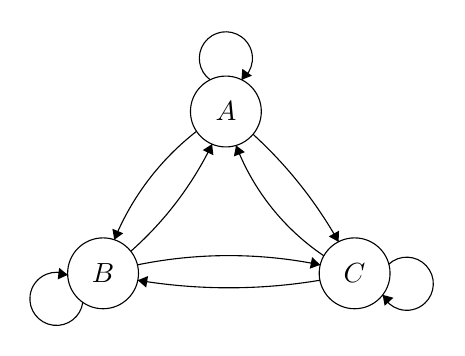
\begin{tikzpicture}[scale=0.15]
		\tikzstyle{every node}+=[inner sep=0pt]
		\draw [black] (23.7,-25.4) circle (3);
		\draw (23.7,-25.4) node {$A$};
		\draw [black] (13.3,-39.1) circle (3);
		\draw (13.3,-39.1) node {$B$};
		\draw [black] (34.6,-39.1) circle (3);
		\draw (34.6,-39.1) node {$C$};
		\draw [black] (14.249,-36.256) arc (157.70826:127.88572:22.39);
		\fill [black] (14.25,-36.26) -- (15.01,-35.71) -- (14.09,-35.33);
		\draw [black] (22.535,-28.163) arc (-25.83943:-48.56659:28.903);
		\fill [black] (22.53,-28.16) -- (21.74,-28.67) -- (22.64,-29.1);
		\draw [black] (16.213,-38.384) arc (101.57892:78.42108:38.549);
		\fill [black] (31.69,-38.38) -- (31,-37.73) -- (30.8,-38.71);
		\draw [black] (31.659,-39.688) arc (-80.52759:-99.47241:46.841);
		\fill [black] (16.24,-39.69) -- (16.95,-40.31) -- (17.11,-39.33);
		\draw [black] (25.997,-27.328) arc (47.64144:29.37151:36.624);
		\fill [black] (33.24,-36.43) -- (33.28,-35.49) -- (32.41,-35.98);
		\draw [black] (31.995,-37.618) arc (-123.95959:-159.02746:19.823);
		\fill [black] (24.56,-28.27) -- (24.38,-29.2) -- (25.31,-28.84);
		\draw [black] (22.377,-22.72) arc (234:-54:2.25);
		\fill [black] (25.02,-22.72) -- (25.9,-22.37) -- (25.09,-21.78);
		\draw [black] (37.487,-38.329) arc (132.69007:-155.30993:2.25);
		\fill [black] (36.97,-40.92) -- (37.14,-41.85) -- (37.88,-41.17);
		\draw [black] (11.585,-41.547) arc (-7.29476:-295.29476:2.25);
		\fill [black] (10.31,-39.23) -- (9.58,-38.63) -- (9.46,-39.62);
	\end{tikzpicture}
\end{center}


จากที่เรียนมาในห้อง เราทราบกันอยู่แล้วว่าความหมายของการนำเมทริกซ์การเปลี่ยนสถานะ 1 ขั้นมาคูณกัน จะได้ผลออกมาเป็นเมทริกซ์การเปลี่ยนสถานะข้าม 2 ขั้น (เช่นเปลี่ยนจากขั้นที่ 1 ไปขั้นที่ 3)
ดังนั้น ถ้าเราอยากหาผลคูณของเมทริกซ์การเปลี่ยนสถานะ สิ่งที่ต้องทำคือหาความน่าจะเป็นในการเดินข้าม 2 ขั้นทุกรูปแบบที่เป็นไปได้

\subsubsection*{การเปลี่ยนสถานะจาก A ในขั้นที่ 1 ไป A ในขั้นที่ 3}
วาดแผนภาพด้านล่าง โจทย์คือ \underline{\textbf{จงเขียนค่าความน่าจะเป็นของการย้ายสถานะของแต่ละเส้น (มี 6 เส้น)}}
\begin{center}
	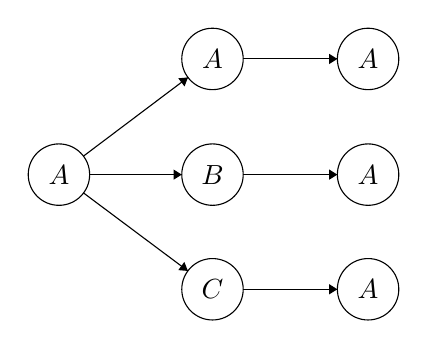
\begin{tikzpicture}[scale=0.13]
		\tikzstyle{every node}+=[inner sep=0pt]
		\draw [black] (11,-31.3) circle (3);
		\draw (11,-31.3) node {$A$};
		\draw [black] (26,-31.3) circle (3);
		\draw (26,-31.3) node {$B$};
		\draw [black] (26,-42.5) circle (3);
		\draw (26,-42.5) node {$C$};
		\draw [black] (26,-20) circle (3);
		\draw (26,-20) node {$A$};
		\draw [black] (41.2,-20) circle (3);
		\draw (41.2,-20) node {$A$};
		\draw [black] (41.2,-31.3) circle (3);
		\draw (41.2,-31.3) node {$A$};
		\draw [black] (41.2,-42.5) circle (3);
		\draw (41.2,-42.5) node {$A$};
		\draw [black] (13.4,-29.49) -- (23.6,-21.81);
		\fill [black] (23.6,-21.81) -- (22.66,-21.89) -- (23.27,-22.69);
		\draw [black] (14,-31.3) -- (23,-31.3);
		\fill [black] (23,-31.3) -- (22.2,-30.8) -- (22.2,-31.8);
		\draw [black] (13.4,-33.09) -- (23.6,-40.71);
		\fill [black] (23.6,-40.71) -- (23.25,-39.83) -- (22.66,-40.63);
		\draw [black] (29,-20) -- (38.2,-20);
		\fill [black] (38.2,-20) -- (37.4,-19.5) -- (37.4,-20.5);
		\draw [black] (29,-31.3) -- (38.2,-31.3);
		\fill [black] (38.2,-31.3) -- (37.4,-30.8) -- (37.4,-31.8);
		\draw [black] (29,-42.5) -- (38.2,-42.5);
		\fill [black] (38.2,-42.5) -- (37.4,-42) -- (37.4,-43);
	\end{tikzpicture}
\end{center}

ด้วยความรู้ในเรื่องความน่าจะเป็น เราจะได้ว่าความน่าจะเป็นรวมของการย้ายสถานะจาก A ข้ามไป A ใน 2 ขั้นถัดไปหาได้จากกฏการคูณและการบวกจากแผนภาพต้นไม้ดังกล่าว โดยที่
\begin{itemize}
	\item เส้นต่อกัน ให้นำค่าความน่าจะเป็นของเส้นมาคูณกัน
	\item หลังจากคิดผลคูณค่าความน่าจะเป็นของแต่ละกิ่งเรียบร้อยแล้ว ให้นำมาบวกกัน
\end{itemize}
เพราะฉะนั้น เราจะได้ว่าความน่าจะเป็นของการเปลี่ยนสถานะจาก A ข้ามไป A ใน 2 ขั้นถัดไปมีค่าเท่ากับ
$$
P(A\rightarrow_2A) = \left(\blank{1cm}\times\blank{1cm}\right) + \left(\blank{1cm}\times\blank{1cm}\right) + \left(\blank{1cm}\times\blank{1cm}\right) = 0.56
$$
ซึ่งมีผลลัพธ์เท่ากับสมาชิกในแถวที่ 1 หลักที่ 1 ที่แทนความน่าจะเป็นของการเปลี่ยนจาก A ไป A ในเมทริกซ์ผลลัพธ์
\subsubsection*{การเปลี่ยนสถานะจาก A ในขั้นที่ 1 ไป B ในขั้นที่ 3}
วาดแผนภาพด้านล่าง โจทย์คือ \underline{\textbf{จงเขียนค่าความน่าจะเป็นของการย้ายสถานะของแต่ละเส้น (มี 6 เส้น)}}
\begin{center}
	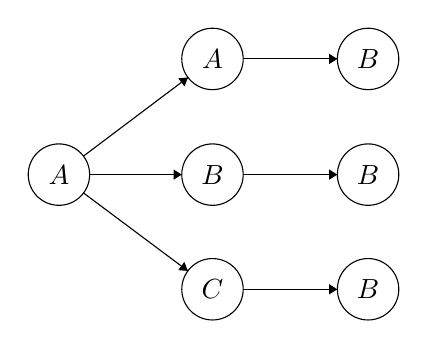
\begin{tikzpicture}[scale=0.13]
		\tikzstyle{every node}+=[inner sep=0pt]
		\draw [black] (11,-31.3) circle (3);
		\draw (11,-31.3) node {$A$};
		\draw [black] (26,-31.3) circle (3);
		\draw (26,-31.3) node {$B$};
		\draw [black] (26,-42.5) circle (3);
		\draw (26,-42.5) node {$C$};
		\draw [black] (26,-20) circle (3);
		\draw (26,-20) node {$A$};
		\draw [black] (41.2,-20) circle (3);
		\draw (41.2,-20) node {$B$};
		\draw [black] (41.2,-31.3) circle (3);
		\draw (41.2,-31.3) node {$B$};
		\draw [black] (41.2,-42.5) circle (3);
		\draw (41.2,-42.5) node {$B$};
		\draw [black] (13.4,-29.49) -- (23.6,-21.81);
		\fill [black] (23.6,-21.81) -- (22.66,-21.89) -- (23.27,-22.69);
		\draw [black] (14,-31.3) -- (23,-31.3);
		\fill [black] (23,-31.3) -- (22.2,-30.8) -- (22.2,-31.8);
		\draw [black] (13.4,-33.09) -- (23.6,-40.71);
		\fill [black] (23.6,-40.71) -- (23.25,-39.83) -- (22.66,-40.63);
		\draw [black] (29,-20) -- (38.2,-20);
		\fill [black] (38.2,-20) -- (37.4,-19.5) -- (37.4,-20.5);
		\draw [black] (29,-31.3) -- (38.2,-31.3);
		\fill [black] (38.2,-31.3) -- (37.4,-30.8) -- (37.4,-31.8);
		\draw [black] (29,-42.5) -- (38.2,-42.5);
		\fill [black] (38.2,-42.5) -- (37.4,-42) -- (37.4,-43);
	\end{tikzpicture}
\end{center}

เพราะฉะนั้น เราจะได้ว่าความน่าจะเป็นของการเปลี่ยนสถานะจาก A ข้ามไป B ใน 2 ขั้นถัดไปมีค่าเท่ากับ
$$
P(A\rightarrow_2B) = \left(\blank{1cm}\times\blank{1cm}\right) + \left(\blank{1cm}\times\blank{1cm}\right) + \left(\blank{1cm}\times\blank{1cm}\right) = \blank{1cm}
$$
	\chapter{การพยากรณ์ (Forecasting)}

การพยากรณ์ (Forecasting) คือการใช้ข้อมูลของสิ่งที่สนใจที่เกิดขึ้นในอดีตเพื่อสร้างแบบจำลองคณิตศาสตร์ที่ใช้ในการคำนวณสิ่งที่สนใจนั้นในอนาคต และในบางตำราจะยังรวมถึงการใช้สภาวะการณ์ที่สำรวจได้ในปัจจุบันรวมไปถึงในอดีตเพื่อทำนาย (Prediction) ค่าที่สนใจ ตัวอย่างเช่น
\begin{itemize}
    \item ฝ่ายขายใช้ยอดขายย้อนหลัง 12 เดือนเพื่อทำนายยอดขายในเดือนถัดไป
    \item ทีมการตลาดต้องการทำนายความต้องการซื้อสินค้าบางอย่างของลูกค้าโดยอาศัยคุณลักษณะต่าง ๆ เช่นเพศ อายุ ฐานเงินเดือน สินค้าที่ซื้อในเดือนที่แล้ว เป็นต้น
\end{itemize}

ในรายวิชานี้ เราจะศึกษา 2 รูปแบบการทำนายหลัก ๆ ดังนี้
\begin{figure}[h]
    \centering
    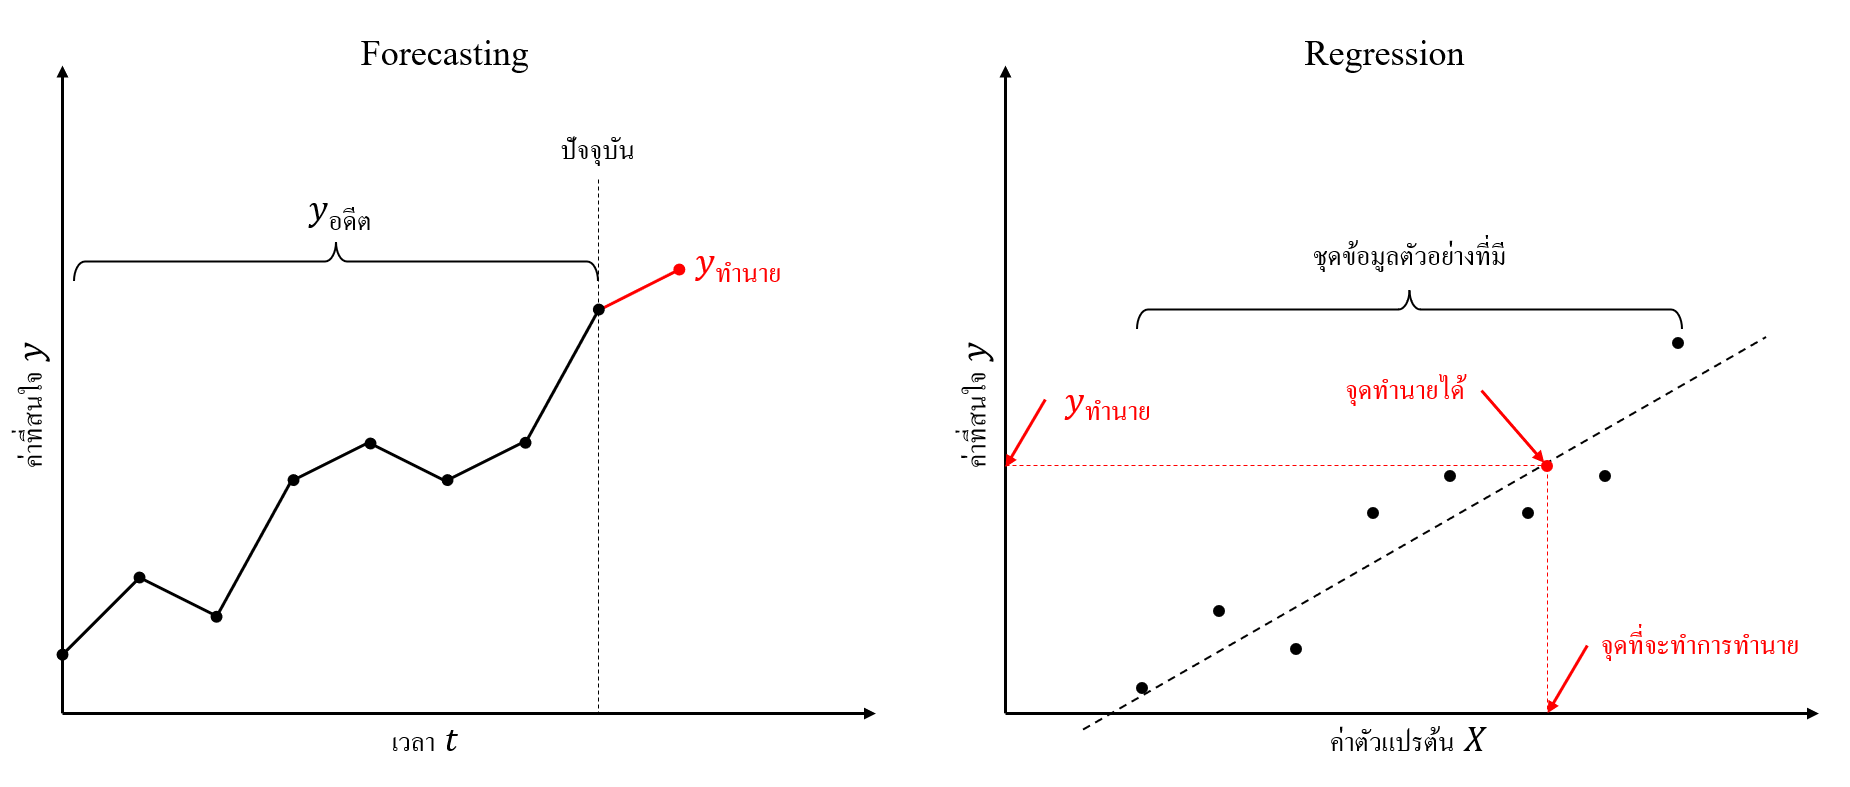
\includegraphics[width=1\linewidth]{forecast_and_regression.png}
    \caption{ความแตกต่างระหว่างตัวแบบอนุกรมเวลาและตัวแบบถดถอย}
\end{figure}
\begin{enumerate}
    \item \textbf{ตัวแบบอนุกรมเวลา} (time series forecasting): เป็นตัวแบบที่อยู่บนสมมติฐานว่าตัวแปรที่เราสนใจมีค่าขึ้นอยู่กับตัวแปรเดียวกันที่เกิดขึ้นในอดีต
    \[
        \hat{y}_{t} \sim y_{t-1}, y_{t-2}, \dots, y_{t-k} 
    \]
    \item \textbf{ตัวแบบการถอดถอย} (regression model): เป็นตัวแบบที่อยู่บนสมมติฐานว่าตัวแปรที่เราสนใจมีค่าขึ้นอยู่กับตัวแปรอื่น ๆ ที่เกิดขึ้นพร้อมกัน (หรือเป็นอยู่)
    \[
        \hat{y}_{t} \sim x_{1,t}, x_{2,t}, \dots, x_{n,t} 
    \]
\end{enumerate}

ทั้งนี้ เราไม่สามารถบอกได้ว่าวิธีการใดเป็นวิธีการที่ดีที่สุด เพราะแต่ละวิธีการ (ที่กำลังจะกล่าวในหัวข้อถัดไป) มีสมมติฐานตั้งต้นที่แตกต่างกัน ขึ้นอยู่กับลักษณะของข้อมูลว่าจะเหมาะสมกับตัวแบบไหน แต่ในทางปฏิบัติ ถ้าไม่มีได้ติดขัดเรื่องปัญหาด้านทรัพยากรในการทำการคำนวณ เรามักจะลองทุกวิธีการและวัดผลเพื่อตรวจสอบเปรียบเทียบความสามารถของแต่ละตัวแบบ (เรียนในหัวข้อสุดท้าย)

%\subsection{ข้อตกลงเรื่องสัญลักษณ์}

\section{ตัวแบบอนุกรมเวลา}
\subsection{วิธีการค่าเฉลี่ยรวม}
\begin{itemize}
    \item เหมาะกับข้อมูลที่มีลักษณะที่ค่อนข้างคงที่ในภาพรวม (ไม่ได้มีแนวโน้มที่เปลี่ยนแปลงไปเช่นตลาดโตขึ้นเรื่อย ๆ)
    \item วิธีการคำนวณ:
    \[
    \hat{y}_{t+1} = \frac{\sum_{i=1}^{t} y_i}{t} = \frac{y_1 + y_2 + \cdots + y_t}{t}
    \]
\end{itemize}

\begin{example}
    {วิธีการค่าเฉลี่ยรวม}{}
    บริษัทหนึ่งมีความต้องการทำนายยอดขายในเดือนที่ 7 โดยที่มียอดขาย 6 เดือนที่ผ่านมาตามตารางด้านล่างนี้ ทั้งนี้ ลองหาค่าทำนายของแต่ละเดือนก่อนหน้าด้วย
\end{example}
\begin{tabular}{|c|c|}
\hline
เดือน & ยอดขาย \\ \hline
1     & 800    \\ \hline
2     & 900    \\ \hline
3     & 800    \\ \hline
4     & 1000   \\ \hline
5     & 1000   \\ \hline
6     & 1300   \\ \hline
\end{tabular}
\newpage
\subsection{วิธีค่าเฉลี่ยเคลื่อนที่ (Moving Average)}
\begin{itemize}
    \item ถ้าข้อมูลระยะยาวไม่คงที่ วิธีการหาค่าเฉลี่ยทั้งหมดอาจจะเอาผลที่ไกลเกินไปมารวม
    \item แต่ถ้าพบว่ามีความคงที่ในระยะสั้น ๆ เช่น ในช่วง 6 เดือนไม่ได้มีการเปลี่ยนแปลงมากนัก เราก็ควรนำแค่ 6 เดือนย้อนหลังมาคิด ซึ่งจะเรียกว่าการหาค่าเฉลี่ยเคลื่อนที่ย้อนหลัง 6 เดือน
    \item วิธีการคำนวณ:
    \[
    \hat{y}_{t+1} = \frac{\sum_{i=t-n+1}^{t} y_i}{n} = \frac{y_{t-n+1} + y_{t-n+2} + \cdots + y_t}{n}
    \]
\end{itemize}
\begin{example}
    {วิธีการค่าเฉลี่ยเคลื่อนที่}{}
    จากตารางเดิม จงหาค่าเฉลี่ยเคลื่อนที่ 3 เดือน และค่าเฉลี่นเคลื่อนที่ 4 เดือนของเดือนทั้งหมดที่เป็นไปได้จนถึงเดือนที่ 7
\end{example}
\begin{tabular}{|c|c|}
\hline
เดือน & ยอดขาย \\ \hline
1     & 800    \\ \hline
2     & 900    \\ \hline
3     & 800    \\ \hline
4     & 1000   \\ \hline
5     & 1000   \\ \hline
6     & 1300   \\ \hline
\end{tabular}\\
~
\vspace{1cm}\\
\noindent\begin{tabular}{|c|c|}
\hline
เดือน & ยอดขาย \\ \hline
1     & 800    \\ \hline
2     & 900    \\ \hline
3     & 800    \\ \hline
4     & 1000   \\ \hline
5     & 1000   \\ \hline
6     & 1300   \\ \hline
\end{tabular}
\newpage
\subsection{วิธีค่าเฉลี่ยเคลื่อนที่ถ่วงน้ำหนัก (Weighted Moving Average)}
\begin{itemize}
    \item เป็นวิธีการที่ต่อยอดมาจากการทำค่าเฉลี่ยนเคลื่อนที่ แต่มีแนวคิดว่าผลกระทบที่ยิ่งห่างออกไปยิ่งควรมีความสำคัญน้อยลง แต่ในขณะที่เหตุการณ์ล่าสุดควรมีผลกระทบมากที่สุด
    \item วิธีการถ่วงน้ำหนักที่ง่ายที่สุดคือไล่ 1, 2, 3, ... จากอดีตสุดมาปัจจุบันสุด
    \item เรียกอีกชื่อว่า \textbf{วิธีปรับเรียบแบบเชิงเส้น}
    \item วิธีการคำนวณ:
    \[
    \hat{y}_{t+1} = \frac{\sum_{i=t-n+1}^{t} (i-t+n)y_i}{\sum_{i=1}^n i} = \frac{1 \cdot y_{t-n+1} + 2 \cdot y_{t-n+2} + \cdots + n \cdot y_t}{1 + 2 + \cdots + n}
    \]
\end{itemize}
\begin{example}
    {วิธีการค่าเฉลี่ยเคลื่อนที่ถ่วงน้ำหนัก}{}
    จากตารางเดิม จงหาค่าเฉลี่ยเคลื่อนที่ถ่วงน้ำหนัก 3 เดือน และค่าเฉลี่นเคลื่อนที่ถ่วงน้ำหนัก 4 เดือนของเดือนทั้งหมดที่เป็นไปได้จนถึงเดือนที่ 7
\end{example}
\begin{tabular}{|c|c|}
\hline
เดือน & ยอดขาย \\ \hline
1     & 800    \\ \hline
2     & 900    \\ \hline
3     & 800    \\ \hline
4     & 1000   \\ \hline
5     & 1000   \\ \hline
6     & 1300   \\ \hline
\end{tabular}\\
~
\vspace{1cm}\\
\noindent\begin{tabular}{|c|c|}
\hline
เดือน & ยอดขาย \\ \hline
1     & 800    \\ \hline
2     & 900    \\ \hline
3     & 800    \\ \hline
4     & 1000   \\ \hline
5     & 1000   \\ \hline
6     & 1300   \\ \hline
\end{tabular}

\newpage
\subsection{วิธีปรับเรียบแบบเอกซ์โพเนเชียล (exponential smoothing)}
\begin{itemize}
    \item เป็นอีกวิธีในการถ่วงน้ำหนัก โดยให้ความสำคัญของค่าล่าสุดเริ่มที่ 1 และลดค่าความสำคัญลงไปแบบ exponential โดยที่ยังมีการนำค่าตั้งแต่จุดเริ่มต้นมาพิจารณา
    \item แต่สูตรการคำนวณถูกจัดให้อยู่ในรูปที่คำนวณได้ง่าย (แค่ต้องคำนวณไต่ลำดับขึ้นมาเรื่อย ๆ) รูปแบบ exponential จึงไม่เห็นอยู่ในสูตร
    \item วิธีการคำนวณ:
    \[
    \hat{y}_{t+1} = \hat{y}_{t} + \alpha(y_t - \hat{y}_{t})
    \]
    หรือ
    \[
    \hat{y}_{t+1} = \alpha y_{t} + (1-\alpha)\hat{y}_t
    \]
    โดยที่ $0 \leq \alpha \leq 1$
    \item ค่า $\alpha$ เป็นค่าที่ต้องกำหนดขึ้นมาตั้งแต่เริ่มตัดสินใจ (เหมือนกับที่เราต้องเลือกว่าจะ moving average หรือ weighted moving average ของกี่เดือน)
\end{itemize}
\begin{example}
    {วิธีปรับเรียบแบบเอกซ์โพเนนเชียล}{}
    จากตารางเดิม จงหาค่าทำนายจากวิธีการปรับเรียบแบบเอกซ์โพเนนเชียล โดยใช้ $\alpha=0.3$ และ $\alpha=0.8$
\end{example}
\begin{tabular}{|c|c|}
\hline
เดือน & ยอดขาย \\ \hline
1     & 800    \\ \hline
2     & 900    \\ \hline
3     & 800    \\ \hline
4     & 1000   \\ \hline
5     & 1000   \\ \hline
6     & 1300   \\ \hline
\end{tabular}\\
~
\vspace{1cm}\\
\noindent\begin{tabular}{|c|c|}
\hline
เดือน & ยอดขาย \\ \hline
1     & 800    \\ \hline
2     & 900    \\ \hline
3     & 800    \\ \hline
4     & 1000   \\ \hline
5     & 1000   \\ \hline
6     & 1300   \\ \hline
\end{tabular}

\newpage
\begin{remark}
    {สาเหตุที่เรียกว่าการปรับเรียบแบบเอกซ์โพเนนเชียล}{}
    รูปแบบสมการที่นิยามมาในด้านบนเรียกว่าการนิยามแบบเวียนเกิด คือการจะหาพจน์ที่ใด ๆ ได้ จะต้องคำนวณให้ทราบค่าพจน์ก่อนหน้าก่อน ดังนั้นจึงจำเป็นต้องคำนวณไล่จากขั้นที่ 1 ขึ้นมาจนถึงขั้นที่ต้องการ แต่ทั้งนี้ เรายังสามารถจัดรูปให้อยู่ในรูปที่ไม่ขึ้นกับพจน์ก่อนหน้าได้ดังนี้
    \begin{align*}
        \hat{y}_{t+1}   &= \alpha y_{t} + (1-\alpha)\hat{y}_t\\
                        &= \alpha y_{t} + (1-\alpha)(\alpha y_{t-1} + (1-\alpha)\hat{y}_{t-1})\\
                        &= \alpha y_{t} + \alpha (1-\alpha) y_{t-1} + (1-\alpha)^2 \hat{y}_{t-1}\\
                        &= \alpha y_{t} + \alpha (1-\alpha) y_{t-1} + \alpha (1-\alpha)^2 y_{t-2} + (1-\alpha)^3 \hat{y}_{t-3}\\
                        &= \alpha y_{t} + \alpha (1-\alpha) y_{t-1} + \alpha (1-\alpha)^2 y_{t-2} + \alpha (1-\alpha)^3 y_{t-3} + (1-\alpha)^4 \hat{y}_{t-4}\\
                        & \quad\vdots \\
                        &= \alpha y_{t} + \alpha (1-\alpha) y_{t-1} + \alpha (1-\alpha)^2 y_{t-2} + \cdots + \alpha (1-\alpha)^{t-2} y_2 + (1 - \alpha)^{t-1} y_1
    \end{align*}
    หรือถ้าเขียนเป็นตัวอย่างแบบตัวเลขชัดเจน จะมีดังนี้
    \begin{align*}
        \hat{y}_1 &= y_1\\
        \hat{y}_2 &= (1 - \alpha)^0 y_1 = y_1\\
        \hat{y}_3 &= \alpha y_2 + (1-\alpha) y_1\\
        \hat{y}_4 &= \alpha y_3 + \alpha (1-\alpha) y_2 + (1-\alpha)^2 y_1\\
        \hat{y}_5 &= \alpha y_4 + \alpha (1-\alpha) y_3 + \alpha (1-\alpha)^2 y_2 + (1-\alpha)^3 y_1
    \end{align*}
    ซึ่งจะเห็นว่า
    \begin{enumerate}
        \item จำนวนพจน์ของค่าจริงที่มาใช้คำนวณจะไม่ถูกกำหนดตายตัวเหมือนวิธีค่าเฉลี่ยเคลื่อนที่แบบอื่นๆ
        \item แต่ความสำคัญก็จะถูกลดทอนลงเรื่อย ๆ จนเข้าใกล้ 0
    \end{enumerate}
    ตัวอย่างกราฟค่าความสำคัญเมื่อใช้ $\alpha = 0.3, 0.5, 0.95, 1$ แสดงการลดแบบ exponential\\
    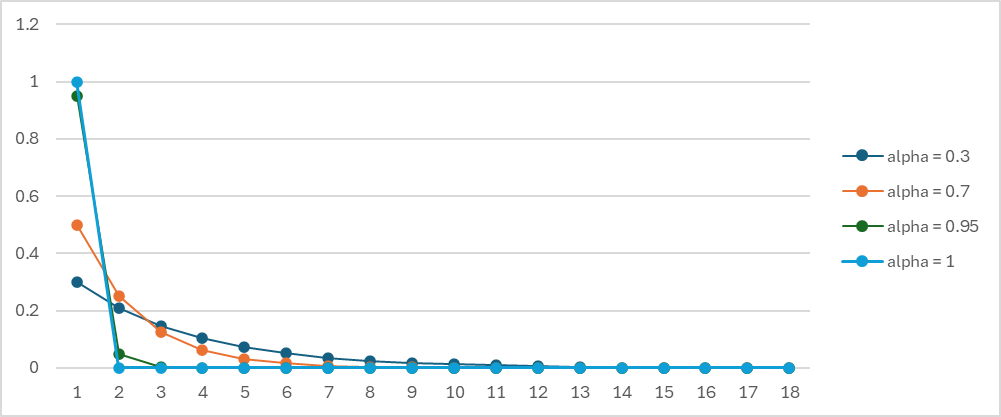
\includegraphics[width=0.9\linewidth]{alpha-expo-smoothing.png}
\end{remark}

\section{ตัวแบบการถดถอยเชิงเส้น}
\begin{itemize}
    \item ตัวแบบการถดถอย (regression) เป็นการสร้างตัวแบบการทำนายโดยอยู่บนสมมติฐานว่าตัวแปรต้นตัวหนึ่ง ($x$) มีความสัมพันธ์เชิงฟังก์ชันกับค่าตัวแปรที่เราสนใจ ($y$)
    \item ในวิชานี้เราสนใจแค่การถดถอยเชิงเส้นตัวแปรเดียว กล่าวคือ มีชุดข้อมูล $(x_1,y_1), (x_2, y_2), \dots, (x_n,y_n)$ ที่มีความสัมพันธ์
    $$
    Y = a_0 + a_1X + \epsilon
    $$
    โดย $a_0, a_1$ เป็นค่าคงที่ และ $\epsilon$ คือพจน์ค่าคาดเคลื่อน
    \item เป้าหมายคือเราต้องการประมาณค่า $a_0 = \alpha_0, a_1 = \alpha_1$ ที่
    $$
    Y \approx \hat{Y} = \alpha_0 + \alpha_1X
    $$
\end{itemize}
\begin{figure}[h]
    \centering
    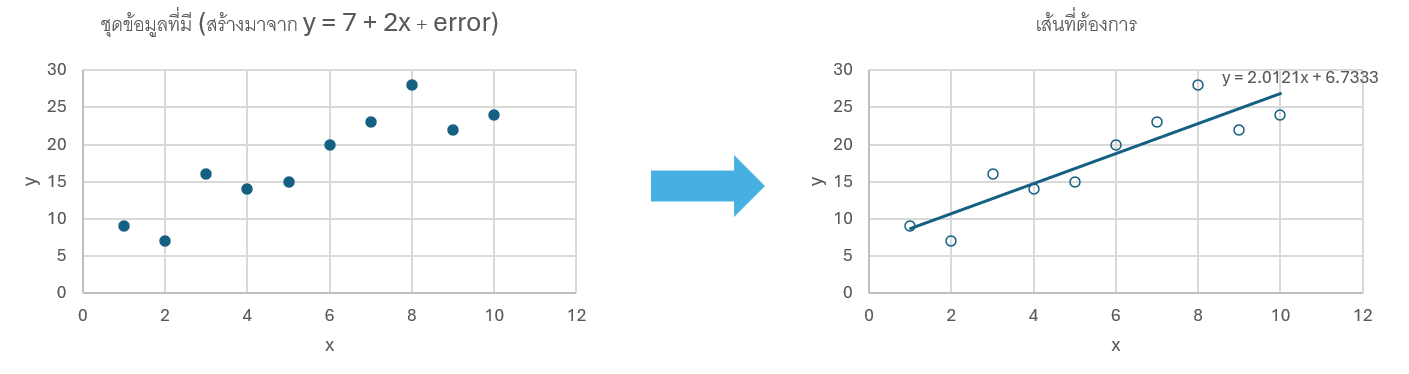
\includegraphics[width=1\linewidth]{regressionSample.png}
\end{figure}

\begin{algorithm}[breakable]
    {}{}
    ค่า $a_0, a_1$ ของตัวแบบการถดถอยเชิงเส้น $Y = a_0 + a_1X + \epsilon$ ของชุดข้อมูล $(x_1,y_1), (x_2, y_2), \dots, (x_n,y_n)$ สามารถประมาณค่าได้ด้วย $\alpha_0, \alpha_1$ (ด้วยวิธีการทางคณิตศาสตร์ที่เรียกว่าวิธีกำลังสองต่ำสุด (Least Squared Error)) ตามสูตร
	\[
        \alpha_1 = \frac{\sum_{i=1}^n(x_i-\bar{x})(y_i-\bar{y})}{\sum_{i=1}^n (x_i - \bar{x})^2},\hspace{1cm} \alpha_0 = \bar{y} - \alpha_1 \bar{x}
	\]
    และจะได้ว่า $\hat{Y} = \alpha_0 + \alpha_1X$ เป็นตัวแบบการถดถอยเชิงเส้นของ $Y = a_0 + a_1X + \epsilon$
    
    โดยขั้นตอนการคำนวณตามสูตรดังกล่าวคือ
   	\begin{enumerate}
   		\item คำนวณหาค่าเฉลี่ย $\bar{x} = \sum_{i=1}^{n}x / n$ และค่าเฉลี่ย $\bar{y} = \sum_{i=1}^{n}y / n$
   		\item $(x_i-\bar{x})$: คำนวณหาผลต่างระหว่างค่า $x$ และค่าเฉลี่ย $\bar{x}$ ของทุกข้อมูล 
   		\item $(y_i-\bar{y})$: คำนวณหาผลต่างระหว่างค่า $y$ และค่าเฉลี่ย $\bar{y}$ ของทุกข้อมูล 
   		\item $(x_i-\bar{x})(y_i-\bar{y})$: นำค่าผลต่างจาก 2 ข้อก่อนหน้ามาคูณกัน
   		\item $\sum_{i=1}^n(x_i-\bar{x})(y_i-\bar{y})$: นำค่าผลคูณของทุกข้อมูลจากขั้นที่ผ่านมามาบวกกัน
   		\item $(x_i-\bar{x})^2$: นำค่าผลต่างที่คำนวณไว้ในขั้นที่ 2 มายกกำลังสอง
   		\item $\sum_{i=1}^n(x_i-\bar{x})^2$: นำค่ากำลังสองของผลต่างในขั้นตอนที่ผ่านมามาบวกกัน
   		\item $\alpha_1=$ ค่าผลบวกจากขั้นตอนที่ 5 หารด้วยค่าผลบวกจากขั้นตอนที่ 7
   		\item $\alpha_0=\bar{y} - \alpha_1 \bar{x}$
   	\end{enumerate}
\end{algorithm}
นักศึกษาสามารถสร้างตารางการคำนวณตามตัวอย่างด้านล่างเพื่อใช้ประกอบการคำนวณได้
\begin{center}
	\begin{tabular}{|c|c|c|c|c|c|}
	\hline
	$x_i$ & $y_i$ & $x_i-\bar{x}$ & $y_i-\bar{y}$ &  $(x_i-\bar{x})(y_i-\bar{y})$ & $(x_i-\bar{x})^2$ \\
	\hline
	$x_1$&$y_1$&&&&\\
	$x_2$&$y_2$&&&&\\
	&&&&&\\
	&&&&&\\
	&&&&&\\
	&&&&&\\
	&&&&&\\
	$x_n$&$y_n$&&&&\\
	\hline
	$\bar{x} = \frac{\sum_{i=1}^{n}x_i}{n}$&$\bar{y} = \frac{\sum_{i=1}^{n}y_i}{n}$&&&$\sum_{i=1}^n(x_i-\bar{x})(y_i-\bar{y})$&$\sum_{i=1}^n(x_i-\bar{x})^2$\\
	\hline
\end{tabular}
\end{center}
\newpage
\begin{example}
    {การถดถอยเชิงเส้น 1 ตัวแปร}{regression1}
    จงประมาณตัวแบบการถดถอยเชิงเส้นของชุดข้อมูลดังตารางด้านล่าง (ข้อมูลเดียวกับรูปตัวอย่าง)
\end{example}
\begin{figure}[h]
    \centering
    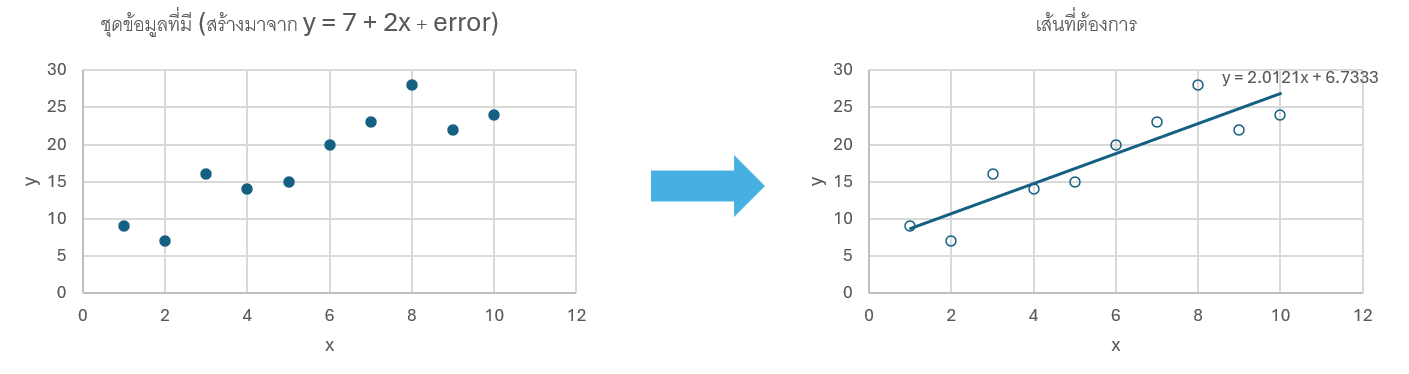
\includegraphics[width=1\linewidth]{regressionSample.png}
\end{figure}
\begin{tabular}{|c|c|}
    \hline
    $x$ & $y$ \\[0.05em] & \\ \hline
    1     & 9   \\[0.05em] & \\ \hline
    2     & 7    \\[0.05em] & \\ \hline
    3     & 16    \\[0.05em] & \\ \hline
    4     & 14   \\[0.05em] & \\ \hline
    5     & 15   \\[0.05em] & \\ \hline
    6     & 20   \\[0.05em] & \\ \hline
    7     & 23  \\[0.05em] &  \\ \hline
    8     & 28  \\[0.05em] &  \\ \hline
    9     & 22   \\[0.05em] & \\ \hline
    10    & 24   \\[0.05em] & \\ \hline
\end{tabular}\\

\section{การประเมิณผลความแม่นยำในการทำนาย}
อย่างที่ได้กล่าวไปก่อนหน้านี้ว่าเราไม่สามารถระบุได้ว่าตัวแบบใดเป็นตัวแบบที่ดีที่สุด เพราะตัวแบบในการทำนายที่ดีขึ้นอยู่กับข้อมูลที่มีว่ามีลักษณะข้อมูลเป็นอย่างไร ตัวแบบเดียวกันอาจจะทำงานได้ดีในชุดข้อมูลหนึ่ง แต่อาจจะทำได้ไม่ดีในอีกชุดข้อมูลหนึ่ง เพราะฉะนั้น ในกระบวนการทำงานจริง จึงต้องมีการวัดผลเพื่อประเมิณความแม่นยำของตัวแบบเพื่อที่จะเปรียบเทียบความสามารถในการทำนายของแต่ละตัวแบบได้ ซึ่งแนวคิดหลักของการวัดผลคือการใช้ค่า\textbf{ความคลาดเคลื่อน} (error) เพื่อเป็นตัวบอกว่าสิ่งที่ตัวแบบทำนายออกมาได้คลาดเคลื่อนออกไปจากค่าจริงเท่าใด
\[
\text{ค่าความคลาดเคลื่อนดิบ} = \left|\text{ค่าที่ตัวแบบทำนายได้} - \text{ค่าจริงจากชุดข้อมูล}\right|
\]
\begin{center}
	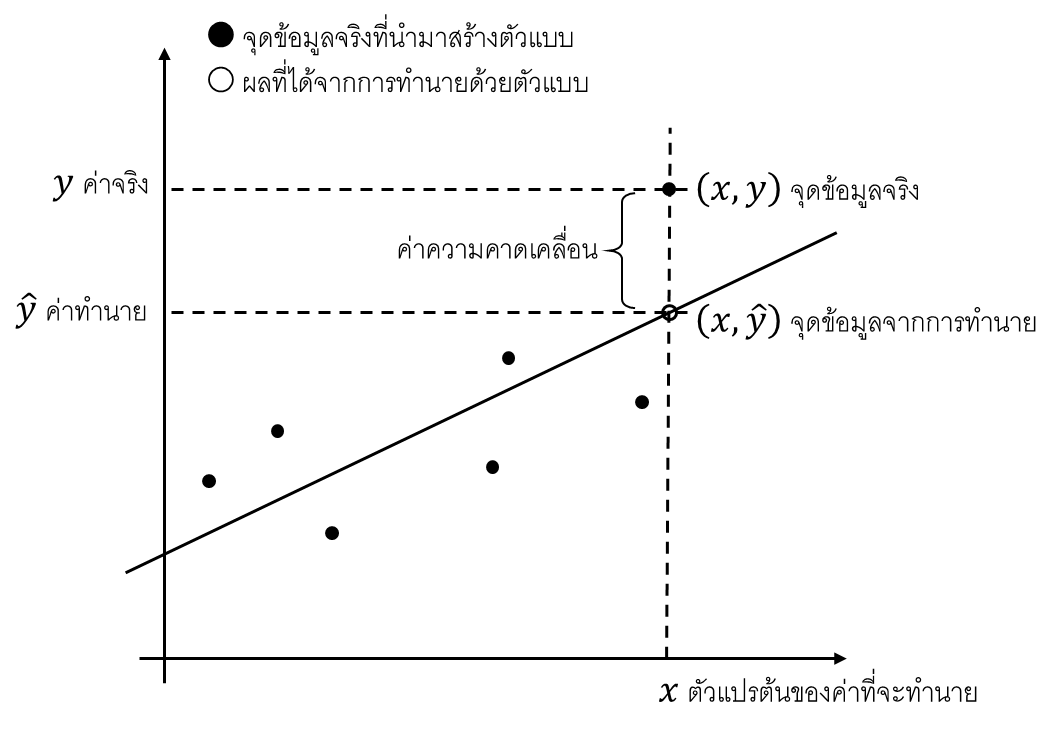
\includegraphics[width=0.5\linewidth]{image/error_in_forecasting}
\end{center}
ในหนังสือเล่มนี้ จะแบ่งการวัดผลออกเป็น 2 รูปแบบหลักได้แก่
\begin{enumerate}
	\item \textbf{การวัดผลด้วยมาตรวัดของข้อมูล}: เป็นการวัดผลที่มีหน่วยออกมาเป็นหน่วยเดียวกันกับข้อมูลที่เราต้องการจะทำนาย โดยต้องการวัดระยะห่าง มีข้อดีในแง่การแสกงค่าคาดเคลื่อนจริง ๆ เช่นทำนายคลาดเคลื่อนไปกี่บาท มักถูกใช้ในการเปรียบเทียบระหว่างตัวแบบต่าง ๆ บนข้อมูลชุดเดียวกัน โดยจะกล่าวถึง
	\begin{itemize}
		\item ค่าเฉลี่ยของความผิดพลาดสัมบูรณ์ (mean absolute error: MAE)
		\item ค่ารากที่สองของค่าเฉลี่ยของความผิดพลาดกำลังสอง (root mean squared error: RMSE)
	\end{itemize}
	\item \textbf{การวัดผลเชิงสัมพัทธ์}: เป็นการวัดผลในเชิงการหาร้อยละเทียบเคียงกับค่าจริงว่าคลาดเคลื่อนไปกี่เปอร์เซนต์ ซึ่งวิธีการนี้มักใช้กับชุดข้อมูลที่ความรุนแรงของการคลาดเคลื่อนขึ้นอยู่กับขนาดของค่าจริง กล่าวคือการคาดเคลื่อนด้วยปริมาณหนึ่งตอนที่ค่าจริงมีค่าน้อย ๆ จะรุนแรงกว่าการคาดเคลื่อนขนาดเดียวกันเมื่อค่าจริงมีค่ามาก ๆ (ตัวอย่างเช่น เงินหาย 9 บาทจาก 10 บาท กับเงินหายไป 9 บาทจาก 1 ล้านบาท) อีกทั้งยังเป็นค่าความคลาดเคลื่อนที่ใช้เพื่อการเปรียบเที่ยบการทำงานของตัวแบบในต่างชุดข้อมูลที่อาจจะมีค่าที่ต้องการทำนายอยู่ในคนละมาตรวัดกัน โดยจะกล่าวถึง
	\begin{itemize}
		\item ค่าเฉลี่ยของความผิดพลาดสัมพัทธ์ (mean absolute percentage error: MAPE)
		\item ค่าเฉลี่ยของความผิดพลาดสัมบูรณ์ที่ปรับมาตราส่วน (mean absolute scaled error: MASE)
	\end{itemize}
\end{enumerate}

\begin{definition}
	{mean absolute error}{}
	\[
	MAE = \frac{1}{n}\sum_{i=1}^{n}{|\hat{y}_i - y_i|}
	\]
\end{definition}

\begin{definition}
	{root mean squared error}{}
	\[
	RMSE = \sqrt{\frac{1}{n}\sum_{i=1}^{n}{(\hat{y}_i - y_i)^2}}
	\]
	และในบางครั้ง อาจมีการใช้ MSE ซึ่งคือ
	\[
	MSE = \frac{1}{n}\sum_{i=1}^{n}{(\hat{y}_i - y_i)^2}
	\]
	แต่สิ่งที่ต้องระวังตอนอ่านค่าคือค่าที่ได้จะอยู่ในหน่วยกำลังสองของหน่วยเดิม (เช่นหน่วย $\text{บาท}^2$) ซึ่งไม่ได้มีความหมายในโลกจริง
\end{definition}

\begin{definition}
	{mean absolute percentage error}{}
	\[
	MAPE = \frac{1}{n}\sum_{i=1}^{n}{\left|  \frac{\hat{y}_i - y_i}{y_i} \right|\times 100\% }
	\]
\end{definition}

\begin{definition}
	{mean absolute scaled error}{}
	สำหรับการทำการถดถอยเชิงเส้นเมื่อเทียบกับการทำนายด้วยการหยิบแต่ค่าเฉลี่ยมาเป็นค่าทำนาย
	\[
	MASE = {\frac{\sum_{i=1}^{n}|\hat{y}_i - y_i|}{\sum_{i=1}^{n}|\bar{y}-y_i|}  }
	\]
	
	สำหรับอนุกรมเวลาเมื่อเทียบกับการทำนายด้วยการหยิบค่าของครั้งก่อนหน้ามาเป็นค่าทำนายของครั้งปัจจุบัน
	\[
	MASE = {\frac{\frac{1}{n}\sum_{i=1}^{n}|\hat{y}_i - y_i|}{\frac{1}{T-1}\sum_{t=2}^{T}|y_t - y_{t-1}|}  }
	\]
	สำหรับการวัดผลด้วย MASE นั้น เราสามารถปรับเปลี่ยนวิธีการประมาณค่าตัวเทียบ (ตัวส่วน) เป็นตัวแบบแบบอื่นได้เช่นกัน เพียงแต่ 2 สูตรด้านบนเป็นการเทียบจากตัวแบบที่ง่ายที่สุดที่มักจะนึกถึงกันเป็นอันดับแรกตอนทำนาย
\end{definition}
\newpage
\begin{example}
	{การวัดผลอนุกรมเวลา}{}
	จากตารางการทำตัวแบบอนุกรมเวลาแบบต่าง ๆ ที่ทำมาในตัวอย่างที่ผ่าน ๆ มา จงวัดผลค่าความคลาดเคลื่อน MAE, RMSE, MAPE, MASE ของแต่ละตัวแบบ โดยสมมติเพิ่มว่าค่าจริงของเดือนที่ 7 มีค่าเท่ากับ 1200 (และเพื่อความสะดวกในการคำนวณ จึงขอปัดค่าทำนายให้เป็นจำนวนเต็ม)
\end{example}

วิธีค่าเฉลี่ย\\
\begin{tabular}{|c|c|c|}
	\hline
	เดือน & ยอดขายจริง & ค่าทำนาย \\ \hline
	1     & 800        & -              \\ \hline
	2     & 900        & 800           \\ \hline
	3     & 800        & 850           \\ \hline
	4     & 1000       & 833           \\ \hline
	5     & 1000       & 875           \\ \hline
	6     & 1300       & 900           \\ \hline
	7     & 1200       & 967           \\ \hline
\end{tabular}
\vspace{1cm}\\
วิธีเฉลี่ยเคลื่อนที่ 3 เดือน\\
\begin{tabular}{|c|c|c|}
	\hline
	เดือน & ยอดขายจริง & ค่าทำนาย \\ \hline
	1     & 800        &   -            \\ \hline
	2     & 900        &  -          \\ \hline
	3     & 800        &   -         \\ \hline
	4     & 1000       & 833           \\ \hline
	5     & 1000       & 900           \\ \hline
	6     & 1300       & 933           \\ \hline
	7     & 1200       & 1100           \\ \hline
\end{tabular}
\vspace{1cm}\\
วิธีเฉลี่ยเคลื่อนที่ 4 เดือน\\
\begin{tabular}{|c|c|c|}
	\hline
	เดือน & ยอดขายจริง & ค่าทำนาย \\ \hline
	1     & 800        &  -             \\ \hline
	2     & 900        &  -          \\ \hline
	3     & 800        &   -         \\ \hline
	4     & 1000       &  -          \\ \hline
	5     & 1000       & 875           \\ \hline
	6     & 1300       & 925           \\ \hline
	7     & 1200       & 1025           \\ \hline
\end{tabular}
\vspace{1cm}\\
วิธีค่าเฉลี่ยถ่วงน้ำหนัก 3 เดือน\\
\begin{tabular}{|c|c|c|}
	\hline
	เดือน & ยอดขายจริง & ค่าทำนาย \\ \hline
	1     & 800        &  -             \\ \hline
	2     & 900        &  -          \\ \hline
	3     & 800        &  -          \\ \hline
	4     & 1000       & 833           \\ \hline
	5     & 1000       & 917           \\ \hline
	6     & 1300       & 967           \\ \hline
	7     & 1200       & 1150           \\ \hline
\end{tabular}
\vspace{1cm}\\
วิธีค่าเฉลี่ยถ่วงน้ำหนัก 4 เดือน\\
\begin{tabular}{|c|c|c|}
	\hline
	เดือน & ยอดขายจริง & ค่าทำนาย \\ \hline
	1     & 800        &   -            \\ \hline
	2     & 900        &   -         \\ \hline
	3     & 800        &  -          \\ \hline
	4     & 1000       &  -          \\ \hline
	5     & 1000       & 900           \\ \hline
	6     & 1300       & 950           \\ \hline
	7     & 1200       & 1100           \\ \hline
\end{tabular}
\vspace{1cm}\\
วิธีปรับเรียบแบบเอ็กโพเนนเชียล โดย $\alpha=0.3$\\
\begin{tabular}{|c|c|c|}
	\hline
	เดือน & ยอดขายจริง & ค่าทำนาย \\ \hline
	1     & 800        & 800              \\ \hline
	2     & 900        & 800           \\ \hline
	3     & 800        & 830           \\ \hline
	4     & 1000       & 821           \\ \hline
	5     & 1000       & 875           \\ \hline
	6     & 1300       & 912           \\ \hline
	7     & 1200       & 1029           \\ \hline
\end{tabular}
\vspace{5cm}\\
วิธีปรับเรียบแบบเอ็กโพเนนเชียล โดย $\alpha=0.8$\\
\begin{tabular}{|c|c|c|}
	\hline
	เดือน & ยอดขายจริง & ค่าทำนาย \\ \hline
	1     & 800        & 800              \\ \hline
	2     & 900        & 800           \\ \hline
	3     & 800        & 880           \\ \hline
	4     & 1000       & 806           \\ \hline
	5     & 1000       & 964           \\ \hline
	6     & 1300       & 975           \\ \hline
	7     & 1200       & 1222           \\ \hline
\end{tabular}
\newpage
\begin{example}
	{การวัดผลการถดถอยเชิงเส้น}{}
	จากตัวอย่างการหาตัวแบบการถดถอยเชิงเส้นในตัวอย่าง \ref{ex:regression1} จงวัดผลความคลาดเคลื่อน MAE, RMSE, MAPE, MASE (ในทำนองเดียวกัน ถ้าเป็นการคำนวณมือให้ปัดเป็นจำนวนเต็มเพื่อคิดเลขได้ จะได้คำนวณได้สะดวก)
\end{example}
\begin{tabular}{|c|c|c|}
	\hline
	$x$ & $y$ & $\hat{y}$\\[0.05em] & &.........\\ \hline
	1     & 9   & \\[0.05em] & &\\ \hline
	2     & 7    & \\[0.05em] & &\\ \hline
	3     & 16    & \\[0.05em] & &\\ \hline
	4     & 14   & \\[0.05em] & &\\ \hline
	5     & 15   & \\[0.05em] & &\\ \hline
	6     & 20   & \\[0.05em] & &\\ \hline
	7     & 23  & \\[0.05em] &  &\\ \hline
	8     & 28  & \\[0.05em] &  &\\ \hline
	9     & 22   & \\[0.05em] & &\\ \hline
	10    & 24  &  \\[0.05em] & &\\ \hline
\end{tabular}

\newpage
\section{การใช้ Excel เพื่อช่วยคำนวณหาตัวแบบต่าง ๆ}
\newpage
	\chapter{ทฤษฎีเกม (Game Theory)}

\section{บทนำ}
\subsection{ความหมายของเกม}
\subsection{จุดแตกต่างจากหัวข้อทฤษฎีการตัดสินใจ}

\section{การวิเคราะห์กลยุทธ์ในเกม}
\subsection{แนวคิดพื้นฐาน: maximin vs. minimax}
\subsection{กลยุทธ์แท้และค่าของเกม}

\section{การวิเคราะห์กลยุทธ์ผสม}

\newpage
\includepdf[pages=-]{Quantitative_Analysis_250907.pdf}

\section{เกณฑ์กลยุทธ์เด่น}
ในกรณีที่มีกลยุทธ์มากกว่า 2 กลยุทธ์ การวิเคราะห์กลยุทธ์ผสมด้วยวิธีที่ศึกษาไปในหัวข้อที่ผ่านมาจะไม่สามารถนำมาใช้ได้ เนื่องจากเป็นการผสมกลยุทธ์แบบ $(p, 1-p)$ ทำให้สามารถคำนวณได้กับแค่กรณี 2 กลยุทธ์เท่านั้น เราจึงทำการลดทอนตารางให้มีขนาดเล็กลงทั้งในแนวแถวและแนวหลัก ซึ่งในบางกรณีอาจจะลดทอนได้จนถึงกรณีที่ฝ่ายใดฝ่ายหนึ่งเหลือกลยุทธ์เดียวและสามารถหาค่าของเกมจากตารางดังกล่าวได้โดยง่าย

เกณฑ์ในการลดทอนคือเกณฑ์การถูกครอบงำโดยกลยุทธ์อื่น โดยที่
\begin{definition}
	{เกณฑ์การถูกครอบงำ}{}
	ในตารางผลตอบแทนของการแข่งขันที่กำหนดให้ \textbf{กลยุทธ์ A ถูกครอบงำโดยกลยุทธ์ B} ถ้าไม่ว่าอีกฝ่ายจะเล่นกลยุทธ์ใดก็ตามค่าของกลยุทธ์ A จะแย่กว่าค่าของกลยุทธ์ B เสมอ ซึ่งถ้าเจอกลยุทธ์ใดก็ตามที่ถูกครอบงำด้วยกลยุทธ์อื่นก็จะสามารถตัดออกจากตัวเลือกการตัดสินใจได้ทันที เพราะไม่มีประโยชน์ที่จะเล่นกลยุทธ์ดังกล่าวแล้ว
\end{definition}
\begin{remark}
	{กลยุทธ์ที่ดีกว่าหรือแย่กว่า}{}
	สมมติให้ตารางผลตอบแทนที่มีเป็นผลตอบแทนของฝ่ายที่เล่นกลยุทธ์ตามแถว กล่าวคือเราจะหา maximin ของแต่ละแถว และหา minimax ของแต่ละหลัก
	\begin{itemize}
		\item ถ้าพิจารณากลยุทธ์ตามแถว (กลยุทธ์ฝ่ายผู้เล่น) กลยุทธ์ที่ดีกว่าคือกลยุทธ์ที่มีค่าผลตอบแทนมากกว่า
		\item ถ้าพิจารณากลยุทธ์ตามหลัก (กลยุทธ์ฝ่ายตรงข้าม) กลยุทธ์ที่ดีกว่าคือกลยุทธ์ที่มีค่าผลตอบแทนน้อยกว่า (เพราะฝ่ายตรงข้ามเสียหายน้อยกว่า)
	\end{itemize}
\end{remark}

\begin{example}
	{ตัวอย่างที่ถูกตัดกลยุทธ์ที่ถูกครอบงำออกจนเหลือกรณีกลยุทธ์บริสุทธ์}{}
	กำหนดให้ตารางผลตอบแทนด้านล่างเป็นตารางผลตอบแทนของ Player 1 ในเกมผลรวมเป็นศูนย์
	\begin{enumerate}
		\item พิจารณาว่าในบรรดากลยุทธ์ของ Player 1 มีกลยุทธ์ใดบ้างที่ถูกครอบงำและถูกครอบงำด้วยกลยุทธ์ใด
		\item จากข้อที่แล้ว ให้ตัดกลยุทธ์ที่ถูกครอบงำทั้งหมดทิ้ง และพิจารณากลยุทธ์ที่ถูกครอบงำในบรรดากลยุทธ์ของ Player 2
		\item ตัดกลยุทธ์ที่ถูกครอบงำออกและวนทำไปเรื่อยๆ จนกว่าจะตัดกลยุทธ์ต่อไม่ได้อีกแล้ว
	\end{enumerate}
	~\\
	\begin{tabular}{|c|c|ccc|}
		\hline
		&   & \multicolumn{3}{c|}{Player 2}                         \\ \hline
		&   & \multicolumn{1}{c|}{X}  & \multicolumn{1}{c|}{Y} & Z  \\ \hline
		\multirow{4}{*}{Player 1} & A & \multicolumn{1}{c|}{1}  & \multicolumn{1}{c|}{0} & 10 \\ \cline{2-5} 
		& B & \multicolumn{1}{c|}{-1} & \multicolumn{1}{c|}{0} & 9  \\ \cline{2-5} 
		& C & \multicolumn{1}{c|}{2}  & \multicolumn{1}{c|}{1} & 8  \\ \cline{2-5} 
		& D & \multicolumn{1}{c|}{-2} & \multicolumn{1}{c|}{0} & 7  \\ \hline
	\end{tabular}
\end{example}

\begin{example}
	{ตัวอย่างที่ถูกตัดกลยุทธ์ที่ถูกครอบงำออกจนเหลือกรณี 2 กลยุทธ์}{}
	กำหนดให้ตารางผลตอบแทนด้านล่างเป็นตารางผลตอบแทนของ Player 1 ในเกมผลรวมเป็นศูนย์ ซึ่งกรณีนี้จะไม่มีกลยุทธ์บริสุทธิ์ จึงต้องทำการผสมกลยุทธ์ จงหาค่าของเกมจากการผสมกลยุทธ์\\
	\begin{tabular}{|c|c|ccc|}
		\hline
		&   & \multicolumn{3}{c|}{Player 2}                         \\ \hline
		&   & \multicolumn{1}{c|}{X}  & \multicolumn{1}{c|}{Y} & Z  \\ \hline
		\multirow{4}{*}{Player 1} & A & \multicolumn{1}{c|}{38}  & \multicolumn{1}{c|}{37} & 39 \\ \cline{2-5} 
		& B & \multicolumn{1}{c|}{25} & \multicolumn{1}{c|}{40} & 41  \\ \cline{2-5} 
		& C & \multicolumn{1}{c|}{35}  & \multicolumn{1}{c|}{32} & 45  \\ \cline{2-5} 
		& D & \multicolumn{1}{c|}{38} & \multicolumn{1}{c|}{30} & 42  \\ \hline
	\end{tabular}
\end{example}
\newpage


\begin{example}
	{ตัวอย่างที่ถูกตัดกลยุทธ์ที่ถูกครอบงำออกแต่ยังเหลือกลยุทธ์มากกว่า 2 กลยุทธ์ (แนวข้อสอบ)}{}
	กำหนดให้ตารางผลตอบแทนด้านล่างเป็นตารางผลตอบแทนของ Player 1 ในเกมผลรวมเป็นศูนย์ ซึ่งกรณีนี้จะไม่มีกลยุทธ์บริสุทธิ์ จึงต้องทำการผสมกลยุทธ์ จงหาค่าของเกมจากการผสมกลยุทธ์\\
	\begin{tabular}{|c|c|ccccc|}
		\hline
		&   & \multicolumn{5}{c|}{Player 2}                         \\ \hline
		&   & \multicolumn{1}{c|}{X}  & \multicolumn{1}{c|}{Y} & \multicolumn{1}{c|}{Z} & \multicolumn{1}{c|}{W} & V \\ \hline
		\multirow{4}{*}{Player 1} 
		& A & \multicolumn{1}{c|}{6}  & \multicolumn{1}{c|}{1} & \multicolumn{1}{c|}{-4} & \multicolumn{1}{c|}{-8} & -3 \\ \cline{2-7} 
		& B & \multicolumn{1}{c|}{-5} & \multicolumn{1}{c|}{-2} & \multicolumn{1}{c|}{2}  & \multicolumn{1}{c|}{6}  & 3  \\ \cline{2-7} 
		& C & \multicolumn{1}{c|}{5}  & \multicolumn{1}{c|}{3} & \multicolumn{1}{c|}{-3} & \multicolumn{1}{c|}{-7} & -2 \\ \cline{2-7} 
		& D & \multicolumn{1}{c|}{4}  & \multicolumn{1}{c|}{2} & \multicolumn{1}{c|}{-5} & \multicolumn{1}{c|}{-9} & -4 \\ \hline
	\end{tabular}
\end{example}
\newpage



\section{การจัดรูปปัญหาเกมผลรวมเป็นศูนย์ให้อยู่ในรูปกำหนดการเชิงเส้น}
	\chapter{ตัวแบบแถวคอย (Queuing Theory)}

\section{บทนำ}
\begin{itemize}
	\item ระบบแถวคอย (การเข้าคิว) คือระบบที่มีผู้ให้บริการและมีผู้มารับบริการ โดยที่ผู้รับบริการอาจจะได้รับบริการทันที หรืออาจจะต้องรอเพื่อรับบริการตามลำดับ
	\item เป้าหมายของบทนี้คือวิเคราะห์และอธิบายระบบการเข้าแถวแบบต่าง ๆ ในแง่ของต้นทุนและแรงงาน
\end{itemize}

\section{โครงสร้างของระบบแถวคอย}
โครงสร้างสำคัญของระบบแถวคอยประกอบด้วย
\begin{enumerate}
	\item ลูกค้า (ผู้มาใช้บริการ): ลักษณะการมาเป็นอย่างไร (อัตราการมา)
	\item รูปแบบของระบบบริการ: มีกี่แถว มีกี่หน่วยบริการ และกระบวนต่อจากการให้บริการของหน่วยบริการเป็นอย่างไร
	\item หน่วยให้บริการ: อัตราการให้บริการเป็นอย่างไร
\end{enumerate}
\begin{figure}[h]
	\centering
	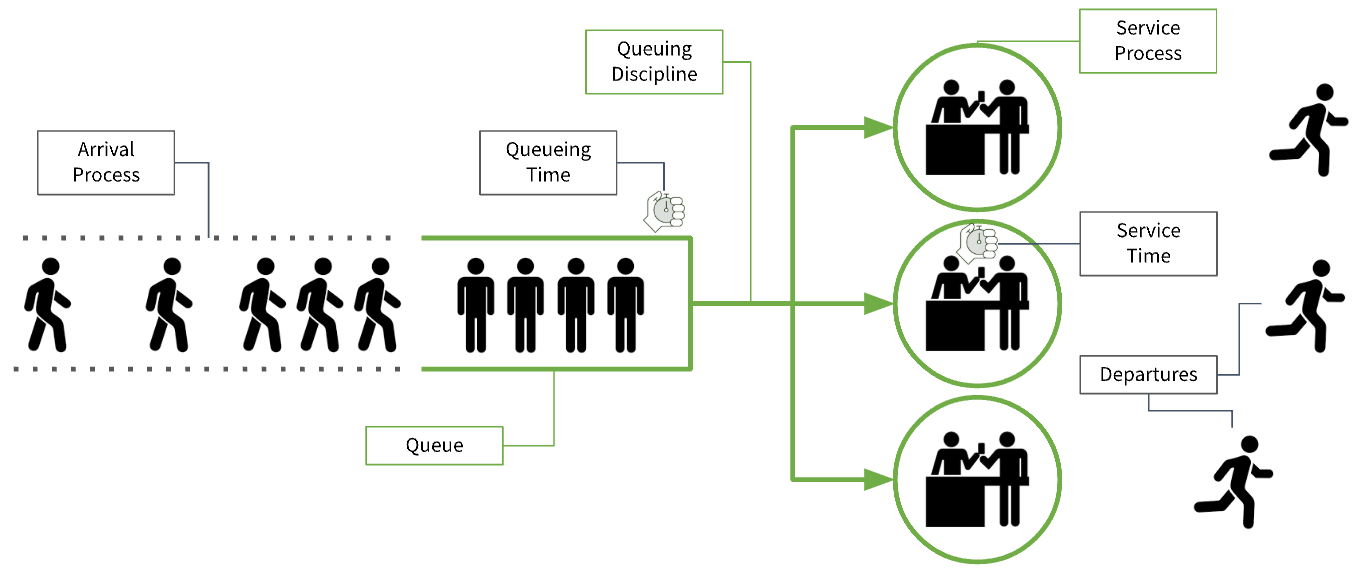
\includegraphics[width=1\linewidth]{image/queue}
\end{figure}

\subsection{ลักษณะของลูกค้า}
จำนวนผู้เข้ารับบริการ:
\begin{itemize}
	\item มีผู้เข้ารับบริการได้ไม่จำกัด
	\item มีผู้เข้ารับบริการได้จำกัด
\end{itemize}

นอกจากประเดินเรื่องความจำกัดของผู้เข้าคิวแล้ว ยังมีประเด็นเรื่องอัตราการมาเข้ารับบริการ (arrival rate) ซึ่งมักสมมติเป็น 2 รูปแบบ
\begin{itemize}
	\item ผู้เข้ารับบริการมาแบบอัตราคงที่
	\item ผู้เข้ารับบริการมาแบบสุ่ม ซึ่ง\underline{มัก}ถูกสมมติให้สุ่มด้วยการแจกแจงแบบปัวซง (Poisson distribution) 
\end{itemize}
ทั้งนี้การแจกแจงความน่าจะเป็นของการมาเข้ารับบริการอาจจะมีการแจกแจงแบบอื่นได้เช่นกันขึ้นอยู่กับสภาพแวดล้อมของแต่ละธุรกิจ

\subsubsection*{Arrival Rate: Poisson distribution}
\begin{property}
	{การแจกแจงปัวซงของอัตราการเข้ารับบริการ}{}
	กำหนดให้ $X$ เป็นตัวแปรสุ่มแทนจำนวนผู้เข้ารับบริการในช่วงระยะเวลาที่กำหนด เราจะกำหนดให้ $X$ มีการแจกแจงแบบปัวซงที่อัตราเฉลี่ยของการเข้ารับบริการมีค่าเท่ากับ $\lambda$ คนต่อหน่วยเวลา กล่าวคือ ความน่าจะเป็นที่จะมีผู้เข้าใช้บริการ $x$ คนมีค่าเท่ากับ
	$$
	P(X = x) = \frac{e^{-\lambda}\lambda^x}{x!}
	$$
\end{property}
\begin{example}
	{Warm-up Poisson}{}
	ในการทำการสำรวจอัตราการเข้าใช้บริการ ณ ร้านค้าแห่งหนึ่งในช่วงระยะเวลา 1 ชั่วโมง ผู้สำรวจพบว่าค่าเฉลี่ยการมาเข้าใช้บริการของบุคคลทั่วไปคือ 10 คน ต่อชั่วโมง กำหนดให้จำนวนผู้ใช้บริการห้างสรรพสินค้าแห่งนี้มีการแจกแจงแบบปัวซง จงหาความน่าจะเป็นต่อไปนี้
	\begin{enumerate}
		\item ความน่าจะเป็นที่จะมีผู้เข้าใช้บริการ 15 คน
		\item ความน่าจะเป็นที่จะมีผู้เข้าใช้บริการไม่เกิน 5 คน
		\item ความน่าจะเป็นที่จะมีผู้เข้าใช้บริการเกิน 5 คน
	\end{enumerate}
\end{example}
\newpage
\subsubsection*{Arrival Time Interval: Exponential distribution}
นอกจากการแจกแจงความน่าจะเป็นของจำนวนผู้เข้าใช้บริการที่มีการแจกแจงแบบปัวซงแล้วนั้น ยังมีการแจกแจงอีกแบบที่มีความสัมพันธ์เกี่ยวข้อกันคือการแจกแจงความน่าจะเป็นของระยะห่างเวลาระหว่างการเข้ามารับบริการ (arrival time interval)
\begin{property}
	{การแจกแจงเอกซ์โพเนเชียลของระยะห่างเวลาระหว่างการเข้ามารับบริการ}{}
	กำหนดให้ $X$ เป็นตัวแปรสุ่มแทนระยะห่างเวลาระหว่างการเข้ามารับบริการ เราจะกำหนดให้ $X$ มีการแจกแจงแบบเอกซ์โพเนนเชียลที่มีอัตราการเข้ามาใช้บริการเท่ากับ \(\lambda\) คนต่อหน่วยเวลา กล่าวคือ ฟังก์ชันการแจกแจงความน่าจะเป็นของตัวแปรสุ่มเวลา $T$ คือ
	\[
	f(t) = \lambda e^{-\lambda t}
	\]
	ซึ่งจะได้ว่าความน่าจะเป็นสะสม $F(a) = P(T\leq a) = 1 - e^{-\lambda a}$

\begin{center}
		\begin{tikzpicture}
		% ---- parameters you can change ----
		\def\lam{0.8} % rate \lambda > 0 (for plotting only)
		\def\a{1.5}   % left-tail cutoff 'a' (shade 0..a)
		% -----------------------------------
		
		\begin{axis}[
			width=11cm, height=7cm,
			domain=0:8, samples=400,
			axis lines=left,
			xmin=0, ymin=0, ymax=1.15*\lam,
			xlabel={$t$}, ylabel={$f(t)$},
			legend style={draw=none, fill=none},
			every axis plot/.append style={thick},
			clip=false
			]
			% pdf curve
			\addplot[name path=exp] {\lam*exp(-\lam*x)};
%			\addlegendentry{$f(t)=\lambda e^{-\lambda t}$}
			
			% baseline for fill
			\path[name path=axis0] (axis cs:0,0) -- (axis cs:\a,0);
			
			% shaded left tail 0..a
			\addplot[fill=gray!30] fill between[of=exp and axis0, soft clip={domain=0:\a}];
			
			% vertical guide at a
%			\draw[dashed] (axis cs:\a,0) -- (axis cs:\a,\lam*exp(-\lam*\a));
			\node[below] at (axis cs:\a,0) {$a$};
%			
%			% annotation of CDF on the tail
			\node[anchor=west] at (axis cs:\a,0.6*\lam)
			{$P(T\le a)=1-e^{-\lambda a}$};
		\end{axis}
	\end{tikzpicture}
\end{center}
\end{property}
\begin{example}
	{Warm-up Exponential}{}
	ในการทำการสำรวจอัตราการเข้าใช้บริการ ณ ร้านค้าแห่งหนึ่งในช่วงระยะเวลา 1 ชั่วโมง ผู้สำรวจพบว่าค่าเฉลี่ยการมาเข้าใช้บริการของบุคคลทั่วไปคือ 10 คน ต่อชั่วโมง กำหนดให้การเข้าใช้บริการเป็นกระบวนการปัวซง จงหาความน่าจะเป็นต่อไปนี้
	\begin{enumerate}
		\item ความน่าจะเป็นที่จะมีผู้เข้ามาใช้บริการภายใน 30 นาที
		\item ความน่าจะเป็นที่จะไม่มีผู้เข้ามาใช้บริการในช่วง 20 นาที
	\end{enumerate}
\end{example}

\newpage
\subsection{ลักษณะของแถวคอย}
\subsubsection{รูปแบบขอองระบบ}
\begin{enumerate}
	\item ระบบช่องทางเดียว-ขั้นตอนเดียว: ตัวอย่างเช่นตู้เอทีเอ็ม 1 ตู้
	\item ระบบช่องทางเดียว-หลายขั้นตอน: ตัวอย่างเช่นการจ่ายยาในโรงพยาบาลขนาดเล็กที่มี 1 เคาท์เตอร์จ่ายยาและ 1 เคาท์เตอร์เก็บเงินที่ผู้ป่วยจะต้องเข้าคิวจ่ายเงินก่อนแล้วค่อยเข้าคิวรับยาในขั้นตอนถัดไป
	\item ระบบหลายช่องทาง-ขั้นตอนเดียว: ตัวอย่างเช่นตู้ซื้อเหรียญโดยสาร MRT บางสถานีที่มีการเข้าคิว 1 แถวเพื่อกระจายคนไปตู้หลายตู้
	\item ระบบหลายช่องทาง-หลายขั้นตอน: ตัวอย่างเช่นแผนกจ่ายยาในโรงพยาบาลใหญ่ที่แต่ละขั้นตอนมีผู้ห้บริการมากกว่า 1 คน 
\end{enumerate}

\subsubsection{ความยาวของแถวคอย}
\begin{enumerate}
	\item จำกัด: เช่นในกรณีที่พื้นที่การเข้าแถวมีจำกัดทำให้เมื่อที่นั่งรอเต็มแล้วจะไม่สามารถรับลูกค้าเข้ามาเพิ่มได้อีกจนกว่าจะมีที่ว่าง เช่นปั๊มน้ำมัน
	\item ไม่จำกัด: เช่นเอกสารที่รอการพิมพ์ หรือระบบการจองที่ไม่ต้องอาศัยพื้นที่ทางกายภาพ
\end{enumerate}

\subsection{ลักษณะของหน่วยให้บริการ}
ในทำนองเดียวกันกับลักษณะการเข้ามาของลูกค้า เราจะสมมติให้เวลาของการให้เป็นบริการเป็นกระบวนการปัวซงเช่นกัน กล่าวคือ
\begin{itemize}
	\item การแจกแจงของเวลาให้บริการเป็นแบบเอกซ์โพเนนเชียล: กำหนดให้ $\mu$ เป็นอัตราการให้บริการโดยเฉลี่ย (คนต่อหน่วยเวลา) จะได้ว่า $f(t)=\mu e^{-\mu t}$ เมื่อ $t>0$ ซึ่งจะได้ตามมาว่า
	\(
	P(T > t) = e^{-\mu t}
	\)
	\item การแจกแจงของจำนวนคนที่ให้บริการได้ในหน่วยเวลาเป็นแบบปัวซง: กล่าวคือ \(P(X=x) = \frac{e^{-\mu}\mu^x}{x!}\)
\end{itemize}
\begin{example}
	{อัตราการ กับ เวลาที่ใช้}{}
	จงหาอัตราของการให้บริการของหน่วยบริการหนึ่งเมื่อกำหนดให้หน่วยบริการนั้นมีใช้เวลาให้บริการ 3 นาทีต่อคน
\end{example}
\newpage
\section{ตัวแบบแถวคอย (เบื้องต้น)}
ทั้งนี้ลักษณะของแถวคอยที่เราจะทำการศึกษาจะมีลักษณะดังต่อไปนี้
\begin{itemize}
	\item แถวคอยขั้นตอนเดียว
	\item หน่วยบริการมีได้ตั้งแต่ $1, 2, \dots$, หรือ $n$ หน่วยบริการ
	\item มาก่อนได้รับบริการก่อน
	\item การมารับบริการและการให้บริการเป็นแบบปัวซง (จำนวนครั้งเป็นปัวซง และระยะเวลาเป็นเอกซ์โพนเนเชียล)
\end{itemize}

\subsubsection{Kendall Notation}
เราจะเขียนรูปแบบแถวคอยเป็นสัญลักษณ์แบบ Kendall Notation ดังนี้
\begin{definition}
	{Kendall Notation}{}
	\[
	A/B/s
	\]
	โดยที่
	\begin{align*}
		A &= \text{การแจกแจงของอัตราการมารับบริการ}\\
		B &= \text{การแจกแจงของอัตราการให้บริการ}\\
		s &= \text{จำนวนหน่วยของผู้ให้บริการ}
	\end{align*}
	และสัญลักษณ์ที่ใช้แทนการแจกแจงมีดังนี้
	\begin{align*}
		M &= \text{แจกแจงแบบปัวซง}\\
		D &= \text{แจกแจงแบบคงที่}\\
		G &= \text{อัตราการให้บริการมีการแจกแจงแบบปกติ}
	\end{align*}
\end{definition}


\subsubsection{สัญลักษณ์ที่ใช้ในการวิเคราะห์แถวคอย}
\begin{definition}[breakable]
	{Notation}{}
	สัญลักษณ์ที่ใช้ในการวิเคราะห์แถวคอยมีดังนี้
	\begin{align*}
		\lambda &= \text{อัตราการเข้ามารับบริการ (จำนวนลูกค้าเฉลี่ยที่เข้ามารับบริการในหนึ่งหน่วยเวลา)}\\
		\mu &= \text{อัตราการให้บริการ (จำนวนลูกค้าเฉลี่ยที่หน่วยบริการสามารถให้บริการแล้วเสร็จในหนึ่งหน่วยเวลา)}\\
		\rho &= \text{ความน่าจะเป็นที่ระบบจะทำงาน (มีผู้รับบริการอยู่ในหน่วยบริการ)}\\
		P_0 &= \text{ความน่าจะเป็นที่ระบบจะว่าง}\\
		L &= \text{จำนวนลูกค้าโดยเฉลี่ยที่อยู่ในระบบ (ทั้งที่กำลังรับบริการและกำลังรอในแถวคอย)}\\
		L_q &= \text{จำนวนลูกค้าโดยเฉลี่ยที่อยู่ในแถวคอย}\\
		W &= \text{เวลาโดยเฉลี่ยที่ลูกค้าเสียไปในการรับบริการในระบบตั้งแต่เข้ามาจนเสร็จ}\\
		W_q &= \text{เวลาโดยเฉลี่ยที่ลูกค้าเสียไปในการรอคอยอยู่ในแถวคอย}\\
		P_n &= \text{ความน่าจะเป็นที่จะมีผู้เข้ามารับบริการจำนวน $n$ คนในระบบแถวคอย}
	\end{align*}
\end{definition}
\subsection{ตัวแบบ M/M/1}
แถวคอยที่มีอัตราการเข้ารับบริการแบบสุ่มแบบกระบวนการปัวซง, มีอัตราการให้บริการแบบปัวซอง และมี 1 หน่วยบริการ (กล่าวคือถ้ายังมี 1 คนใช้บริการอยู่คนที่เหลือต้องเข้าแถวคอยจนกว่าจะใช้บริการเสร็จและออกจากหน่วยบริการ)
\begin{theorem}
	{การวิเคราะห์เชิงปริมาณของแถวคอยแบบ M/M/1}{}
	\begin{align*}
		\rho &= \frac{\lambda}{\mu}, \qquad P_0 = 1 - \frac{\lambda}{\mu}, \qquad P_n = P_0\left(\frac{\lambda}{\mu}\right)^n \\
		L &= \frac{\lambda}{\mu - \lambda}, \qquad L_q = \frac{\lambda^2}{\mu (\mu - \lambda)} \\
		W &= \frac{1}{\mu - \lambda}, \qquad W_q = \frac{\lambda}{\mu(\mu - \lambda)}
	\end{align*}
	โดยทีสมมติฐานของตัวแบบนี้คือ $\lambda < \mu$
\end{theorem}
จริง ๆ แล้วสูตรเหล่านี้มีที่มาจากการใช้การคำนวณเชิงความน่าจะเป็น (ความน่าจะเป็น, ตัวแปรสุ่ม, การแจกแจงความน่าจะเป็นไม่ต่อเนื่อง, ค่าคาดหวัง) นักศึกษาที่แม่นในส่วนของการคำนวณเหล่านี้จะสามารถคำนวณตัวแปรต่าง ๆ ได้ด้วยตัวเองโดยที่ไม่จำเป็นต้องรู้สูตรเหล่านี้ก็ได้

%\begin{remark}
%	{ที่มาของสูตร}{}
%	กำหนดให้
%	\paragraph*{ความน่าจะเป็นที่ระบบจะทำงาน ($\rho$)} คือความน่าจะเป็นที่หน่วยบริการกำลังให้บริการผู้เข้ารับบริการอยู่ ซึ่งสามารถคำนวณหาได้โดยง่าย
%\end{remark}
\newpage
\begin{example}
	{M/M/1}{}
	บริการถ่ายเอกสารที่ร้านแห่งหนึ่งมีเครื่องถ่ายเอกสาร 1 เครื่องให้บริการแบบมาก่อนได้ก่อน โดยที่ลูกค้าที่เข้ามาเพื่อถ่ายเอกสารจะเข้ามาแบบสุ่มปัวซงในอัตรานาทีละ 2 คน ถ้าเวลาที่พนักงานประจำเครื่องถ่ายเอกสารให้บริการลูกค้ามีการแจกแจงแบบเอกซ์โพเนนเชียลด้วยค่าเฉลี่ย 1/4 นาทีต่อคน
	จงวิเคราะห์ระบบแถวคอยของบริการเครื่องถ่ายเอกสาร
\end{example}
\newpage
%\begin{example}
%	{จัดรูปสูตรให้อยู่ในรูปที่จำง่ายขึ้น}{}
%	สูตรที่ให้มาตามทฤษฎีบทเป็นสูตรที่ถูกจัดรูปให้สามารถคำนวณได้โดยใช้แค่ $\lambda$ และ $\mu$ ซึ่งอาจจะทำให้รู้สึกว่าจำได้ยาก เราจึงจะมาจัดรูปสูตรให้จำได้ง่ายขึ้นโดยใช้ความหมายเชิงปริมาณเข้ามาช่วย
%	
%	จงบอกเหตุผลว่าทำไมถึงได้สูตรดังต่อไปนี้ในเชิงความหมายเชิงปริมาณ
%	\begin{enumerate}
%		\item $P_0 = 1 - \rho$
%		\item $P_n=P_0\rho^n$
%		\item $L=\frac{\rho}{1 - \rho}$
%		\item $L_q = \rho L$
%	\end{enumerate}
%\end{example}
%\newpage
\begin{example}
	{M/M/1}{food}
	ร้านค้าแห่งหนึ่งกำลังวางแผนพัฒนาเรื่องการรอคิวของลูกค้าเพื่อไม่ให้ลูกค้าต้องรอคิวนานจึงได้ทำการวิเคราะห์พฤติกรรมลูกค้าและพบว่าจำนวนลูกค้าที่เข้ามาซื้อสินค้าโดยเฉลี่ยจะอยู่ที่ 20 คนต่อชั่วโมงและมีการแจกแจงแบบปัวซอง ในส่วนของทางร้าน พนักงานของร้านสามารถให้บริการคิดชำระเงินได้เฉลี่ย 1 คนต่อ 2 นาทีและมีการแจกแจงของเวลาการให้บริการแบบเอ็กซ์โพเนนเชียล ปัจจุบันทางร้านมีพนักงาน 1 คน จงวิเคราะห์แถวคอยของร้านค้าแห่งนี้ 
\end{example}
\newpage

\subsection{ตัวแบบ M/M/s}
\begin{theorem}
	{การวิเคราะห์เชิงปริมาณของแถวคอยแบบ M/M/s}{}
	\begin{align*}
		\rho &= \frac{\lambda}{s\mu}, \qquad 
		P_0 = \frac{1}{\sum_{n=0}^{s-1} \frac{(\lambda/\mu)^n}{n!} + \left[ \frac{(\lambda/\mu)^s}{s!} \frac{s\mu}{s\mu - \lambda} \right]}\\
		P_n &= \begin{cases}
			P_0\frac{(\lambda/\mu)^n}{n!} &\text{เมื่อ\quad} n\leq s\\
			P_0\frac{(\lambda/\mu)^n}{s!s^{n-s}} &\text{เมื่อ\quad} n > s
		\end{cases}\\
		L_q &= P_0\left[\frac{(\lambda/\mu)^s \rho}{s!(1-\rho)^2}\right], \qquad L = L_q + \frac{\lambda}{\mu}\\
		W_q &= \frac{L_q}{\lambda}, \qquad W = W_q + \frac{1}{\mu}
	\end{align*}
	โดยทีสมมติฐานของตัวแบบนี้คือ $\lambda < s\mu$
\end{theorem}
\begin{example}
	{M/M/s}{}
	บริการถ่ายเอกสารที่ร้านแห่งหนึ่งมีเครื่องถ่ายเอกสาร 5 เครื่องให้บริการแบบมาก่อนได้ก่อน โดยที่ลูกค้าที่เข้ามาเพื่อถ่ายเอกสารจะเข้ามาแบบสุ่มปัวซงในอัตรานาทีละ 2 คน ถ้าเวลาที่พนักงานประจำเครื่องถ่ายเอกสารให้บริการลูกค้ามีการแจกแจงแบบเอกซ์โพเนนเชียลด้วยค่าเฉลี่ย 1/4 นาทีต่อคน
	จงวิเคราะห์ระบบแถวคอยของบริการเครื่องถ่ายเอกสาร
\end{example}
\newpage

\subsection{ตัวแบบ M/G/1}
(ข้ามสำหรับ 720201)
\subsection{ตัวแบบ M/D/1}
(ข้ามสำหรับ 720201)
\section{ตัวแบบแถวคอย (ทฤษฎี)}
(ข้ามสำหรับ 720201)

\section{การวิเคราะห์ระบบแถวคอยเพื่อการตัดสินใจทางธุรกิจ}
ชัดเจนว่าวิธีการหนึ่งที่จะทำให้ลูกค้าไม่ต้องรอคอยคือการเพิ่มหน่วยบริการเข้าไปให้มากพอ หรือมากกว่าลูกค้าที่เข้ามา ก็จะทำให้ลูกค้าทุกคนสามารถได้รับบริการได้ทันที ทว่าวิธีการดังกล่าวอาจจะเป็นไปไม่ได้เพราะใช้ต้นทุนสูงหรือทรัพยากรไม่เพียงพอ (เช่นพื้นที่ร้าน) เราจึงต้องทำการ trade-off กันระหว่างจำนวนหน่วยบริการกับต้นทุนที่ใช้

ทั้งนี้ ต้นทุนที่จะนำมาพิจารณาในการวิเคราะห์แถวคอยมี 2 หมวดดังนี้
\begin{enumerate}
	\item \textbf{ต้นทุนการให้บริการ} (service cost): เช่นค่าแรงงาน ค่าเช่าสถานที่ ที่แปรผันตรงกับจำนวนหน่วยบริการ กล่าวคือ ยิ่งเพิ่มหน่วยบริการมากขึ้น ก็จะใช้ต้นทุนมากขึ้นเรื่อย ๆ
	\item \textbf{ต้นทุนในการรอคอยของลูกค้า} (waiting cost): เป็นค่าเสียหายที่เกิดจากการรอคอยที่ยิ่งลูกค้ารอคอยนานเท่าไหร่ก็จะยิ่งมีค่าใช้จ่ายมากขึ้นเท่านั้น เช่นการประเมิณความพึงพอใจของลูกค้า หรือต้นทุนของบริการเพิ่มเติมที่ลูกค้าได้รับขณะรอคิว (เช่นร้าน Haidilao มีบริการทำเล็บหรือขนมฟรีของลูกค้าที่กำลังรอคิว)
\end{enumerate}
\begin{align*}
	\text{ค่าใช้จ่ายรวม} &= \text{ต้นทุนการให้บริการ} + \text{ต้นทุนการรอคอยของลูกค้า}\\
				TC &= s\cdot C_s + L\cdot C_w 
\end{align*}

\begin{tikzpicture}
	\begin{axis}[
%		axis lines=middle,
		xmin=-0.5, xmax=5,
		ymin=-0.5, ymax=6,
		samples=200,
		domain=0.01:5,   % to avoid x=0 singularity
		legend style={at={(1,1)},anchor=north east},
		xlabel={\textbf{จำนวนหน่วยบริการ}},
		ylabel={\textbf{ค่าใช้จ่าย}}
		]
		
		% (1) y = 1/x
		\addplot[blue, thick] {1/x};
%		\addlegendentry{$y = \tfrac{1}{x}$}
		
		% (2) y = x
		\addplot[red, thick] {x};
%		\addlegendentry{$y = x$}
		
		% (3) y = x + 1/x
		\addplot[green!60!black, thick, dashed] {x + 1/x};
%		\addlegendentry{$y = x + \tfrac{1}{x}$}
		
	\end{axis}
\end{tikzpicture}
\subsection{การกำหนดจำนวนหน่วยบริการ}
โจทย์ที่มักจะถูกถามเป็นอันดับแรกคือเราควรจะทำหน่วยบริการกี่หน่วยดีเพื่อให้เพียงพอที่จะทำให้ลูกค้าพอใจโดยที่ไม่ต้องใช้ต้นทุนเยอะจนเกินไป ซึ่งวิธีการคือการวิเคราะห์หาจุดต่ำสุดของค่าใช้จ่ายรวม
แต่ในทางปฏิบัติ เนื่องจากเราต้องการหาจุดเหมาะสุดของตัวแปรเดียวที่เป็นจำนวนนับ จึงเป็นการง่ายที่จะทำการวิเคราะห์หาต้นทุนรวมของ M/M/1, M/M/2, ... ไปเรื่อย ๆ จนเจอจุดที่ให้ค่าต่ำสุด (ลดลงเรื่อย ๆ จนเจอจุดที่เพิ่มอีกหน่วยแล้วมีต้นทุนมากขึ้น)
\begin{example}
	{}{food2}
	จากตัวอย่าง \ref{ex:food} ที่จำนวนลูกค้าที่เข้ามาซื้อสินค้าโดยเฉลี่ยจะอยู่ที่ 20 คนต่อชั่วโมงและมีการแจกแจงแบบปัวซอง, พนักงานของร้านสามารถให้บริการคิดชำระเงินได้เฉลี่ย 1 คนต่อ 2 นาทีและมีการแจกแจงของเวลาการให้บริการแบบเอ็กซ์โพเนนเชียล สมมติว่าปัจจุบันมีพนักงาน 3 คนอยู่แล้ว จงหาว่าร้านนี้ควรจ้างพนักงานบริการชำระเงินเพิ่มอีกกี่คนมาทำงาน
\end{example}
\newpage

\subsection{การตัดสินใจจัดรูปแบบแถวคอย}
\begin{example}
	{}{}
	จากตัวอย่าง \ref{ex:food2} มีนักวิเคราะห์เสนอว่าแทนที่จะเพิ่มจำนวนพนักงานให้ลองเปลี่ยนรูปแบบเป็นแต่ละพนักงานมีแถวคอยเป็นของตัวเอง และลูกค้าที่เข้ามาจะกระจายตัวกันตามแถวคอยทั้ง 3 แถว กล่าวคือลองเปลี่ยนจาก M/M/3 เป็น M/M/1 ทั้งหมด 3 ระบบอิสระจากกัน จงวิเคราะห์ต้นทุนรวมของระบบใหม่นี้
\end{example}
\newpage

\subsection{การตัดสินใจในลักษณะอื่น ๆ}
\begin{example}
	{}{}
	บริษัทโลจิสติกแห่งหนึ่งให้บริการทั่วไปเกี่ยวกับการขนส่งและจัดเก็บสินค้า โดยปัจจุบันมีโกดังเก็บสินค้าเพียงแห่งเดียว ซึ่งมีที่เทียบรถบรรทุกเพื่อขนส่งสินค้าขึ้นลงได้ครั้งละ 1 คัน รถเข้ามาเฉลี่ยทุก ๆ 40 นาที แจกแจงแบบเอ็กซโพเนนเชียล การขนสินค้าขึ้นลงใช้เวลาเฉลี่ยคันละ 30 นาที แจกแจงแบบเอ็กซโพเนนเชียล ถ้าบริษัทต้องการให้รถแต่ละคันใช้เวลาในระบบการขนถ่ายสินค้าไม่เกินคันละ 1 ชั่วโมง ควรใช้เวลาในการขนสินค้าคันละกี่นาที
\end{example}
\newpage


%\section{การวิเคราะห์แถวคอยโดยกระบวนการมาร์คอฟ}
	\chapter{ปัญหาการหาค่าเหมาะสุดต่าง ๆ ในเชิงธุรกิจ (Optimization Problem in Business)}
\section{Zero-sum game as Linear Programming}
\section{Transportation Problem}
\section{Scheduling Problem}
\section{Matching Problem}


	
	\begin{appendices}               %%%%%%%%%%%%%%%%%%    (COMMENT IF NOT NEEDED)
		% !TEX root = ../BookTemplate.tex
%%%%%%%%%%%%%%%%%%%%%%%%%%%%%%%%%%%%%%%%%%%%%%%%%%%%%%%%%%%%%%%%%%%%%%%%%%%%%%%%%%
\newgeometry{
	top=3cm,
	bottom=3cm,
	left=75pt,
	right=50pt,
	marginparsep=0cm,
	marginparwidth=0cm,
	voffset=0pt,
	hoffset=0pt,
	headheight=0pt,
	headsep=0pt,
	footskip=14pt,
	footnotesep=0pt
}

%%%%%%%%    (APPENDICES TOC)
\addtocontents{toc}{
  \protect\vspace{25pt}
  \protect\noindent\qquad\qquad\bfseries\AppendixPart
  \protect\par
  \protect\vspace{10pt}}
\titlecontents{chapter}[4pc]
{\addvspace{16pt}\bfseries\thecontentslabel}{\hspace{.5cm}}{}
{\color{black!50}\;\;\dotfill\;\bfseries\color{black}\PageName\, \thecontentspage}

%%%%%%%%
\part*{Appendices}
\restoregeometry

%%%%%%%%    (APPENDICES PAGE FORMAT)
\fancypagestyle{fancyapp}{
\renewcommand{\headrulewidth}{0.25pt}
	\fancyhead[LE, RO]{\small\parbox{.45\textwidth}{\checkoddpage
\ifoddpage \raggedleft \else \raggedright \fi \bfseries\nouppercase{\leftmark}}\vspace{.065cm}}
	\fancyhead[LO, RE]{\small\parbox{.45\textwidth}{\checkoddpage
\ifoddpage \raggedright \else \raggedleft \fi \nouppercase{\rightmark}}\vspace{.065cm}}
	\fancyfoot[LE,RO]{\small\thepage}
	\fancyfoot[C]{}
	\fancyfoot[LO,RE]{\small \EMail}}

\pagestyle{fancyapp}    %%%%%%%%%%%%%%%          (DO NOT EDIT)
		\setcounter{page}{1}
		% !TEX root = ../BookTemplate.tex
%%%%%%%%%%%%%%%%%%%%%%%%%%%%%%%%%%%%%%%%%%%%%%%%%%%%%%%%%%%%%%%%%%%%%%%%%%%%%%%%%%
\chapter{คณิตศาสตร์สำหรับการวิเคราะห์เชิงปริมาณ}

ในบทแรก เราจะเริ่มจากการปูพื้นฐานคณิตศาสตร์ที่จำเป็นจะต้องใช้ในการเรียนรู้เนื้อหาวิชาการวิเคราะห์เชิงปริมาณกันก่อน
ทั้งนี้นักศึกษาไม่จำเป็นจะต้องศึกษาทั้งบทภายในครั้งเดียว เนื่องจากแต่ละบทนั้นจะมีคณิตศาสตร์ที่ต้องใช้แตกต่างกันไป นักศึกษาสามารถใช้บทนี้เป็นนบททบทวนก่อนขึ้นเนื้อหาหลักในแต่ละบทได้

สำหรับทางอาจารย์ผู้สอนนั้น ไม่ควรที่จะใช้บทนี้เป็นบทเรียนหลักที่สอนทั้งหมดภายในคราวเดียว เนื่องจากจนกว่าจะถึงตอนที่นักศึกษาจะต้องใช้จริงนั้น นักศึกษาเองก็อาจจะจำรายละเอียดไม่ได้แล้ว
ดังนั้น ทางผู้เขียนจึงขอแนะนำว่าให้หยิบไปบางส่วนขึ้นกับเนื้อหาหลักที่กำลังจะสอน และไม่ควรมีการออกสอบเก็บคะแนนสำหรับบทนี้ เนื่องจากเป็นความรู้พื้นฐานของเนื้อหาหลัก

อาจารย์ผู้สอนหรือนักศึกษาที่ศึกษาด้วยตัวเองสามารถใช้แผนภาพด้านล่างนี้เป็นแนวทางในการศึกษาในแต่ละหัวข้อ:

\begin{center}
\resizebox{\textwidth}{!}{\begin{tikzpicture}[
  font=\footnotesize,
  box/.style={rectangle, draw, text width=3.2cm, align=center, minimum height=1.2cm},
  arrow/.style={-{Stealth}, thick},
  node distance=1.2cm and 1.5cm
]

% กล่องเหตุผลเชิงปริมาณด้านล่าง
\node[box, fill=yellow!20] (reason) at (0,0) {เหตุผลเชิงปริมาณ};

% กลุ่มบทหลักแนวนอน
\node[box, fill=green!15, above=2.3cm of reason, xshift=-6.5cm] (ch2) {บทที่ 2\\โปรแกรมเชิงเส้น};
\node[box, fill=blue!10, right=1.5cm of ch2] (ch3) {บทที่ 3\\จำลองสถานการณ์};
\node[box, fill=blue!10, right=1.5cm of ch3] (ch4) {บทที่ 4\\การตัดสินใจ};
\node[box, fill=blue!10, right=1.5cm of ch4] (ch5) {บทที่ 5\\ทฤษฎีเกม};
\node[box, fill=blue!10, right=1.5cm of ch5] (ch6) {บทที่ 6\\ความน่าจะเป็น};
\node[box, fill=blue!10, right=1.5cm of ch6] (ch7) {บทที่ 7\\แถวคอย};

% คณิตศาสตร์พื้นฐานด้านล่างซ้าย
\node[box, below=1.5cm of ch2] (linear) {ระบบสมการ};
\node[box, below=1.5cm of ch5] (matrix) {เมทริกซ์};
\node[box, below=1.5cm of ch6] (prob) {ความน่าจะเป็น};

% ลูกศรจากคณิตศาสตร์พื้นฐาน
\draw[arrow] (linear.north) -- (ch2.south);
\draw[arrow] (matrix.north) -- (ch2.south);
\draw[arrow] (matrix.north) -- (ch5.south);
\draw[arrow] (prob.north) -- (ch3.south);
\draw[arrow] (prob.north) -- (ch4.south);
\draw[arrow] (prob.north) -- (ch6.south);
\draw[arrow] (prob.north) -- (ch7.south);

% ลูกศรจากเหตุผลเชิงปริมาณ
\foreach \x in {ch2, ch3, ch4, ch5, ch6, ch7}
  \draw[draw=red, dashed, -{Stealth}, thick] (reason.north) -- (\x.south);

\end{tikzpicture}}
\end{center}

\noindent จากแผนภาพจะเห็นว่าหัวข้อการให้เหตุผลเชิงปริมาณเป็นเนื้อหาสำคัญของบทนี้ที่จะข้ามไม่ได้ เนื่องจากเป็นบทที่ว่าด้วยทักษะการแปลปัญหาโลกจริงให้เป็นปัญหาทางคณิตศาสตร์ หรือกล่าวได้ว่าเป็นหัวข้อเกี่ยวกับ mathematical literacy ซึ่งจากประสบการณ์ของผู้เขียนนั้น พบว่านักเรียนนักศึกษาส่วนใหญ่ที่เรียนหัวข้อทางคณิตศาสตร์ หรือหัวข้อประยุกต์ทางคณิตศาสตร์ไม่เข้าใจ ไม่ได้เกิดจากการเรียนดนื้อหาในหัวข้อไม่เข้าใจ แต่เกิดจากการที่ไม่เข้าใจตั้งแต่แนวคิดตั้งต้นที่จะเชื่อมปัญหาในโลกจริงให้กลายเป็นปัญหาทางคณิตศาสตร์และใช้เครื่องมือทางคณิตศาสตร์เข้าไปช่วยแก้ปัญหา ซึ่งทางผู้เขียนค่อนข้างมีความเชื่อว่าสิ่งที่ยากไม่ใช่การเรียนเครื่องมือคณิตศาสตร์ เพราะอยากน้อยก็ใช้วิธีจำไปสอบ หรือตอนทำงานจริงก็เปิดคู่มือทำตามได้ แต่สิ่งที่ยากจริง ๆ คือการที่จะนำคณิตศาสตร์และปัญหาจริงมาเชื่อมโยงกันอย่างไร ดังนั้นจึงขอเน้นย้ำว่าหัวข้อการให้เหตุผลเชิงปริมาณนั้น ถึงแม้จะอยู่หัวข้อสุดท้ายของบท แต่ก็ไม่ควรละเลย

\newpage
\section{ระบบสมการเชิงเส้น}\label{section:linear}
ในบทที่ \ref{chapter:linprog} เราจะเรียนเกี่ยวกับการหาค่ามากสุดหรือน้อยสุด (เรียกว่าการทำ optimization) กับปัญหาที่ทั้งฟังก์ชันจุดประสงค์และเงื่อนไขอยู่ในรูปแบบที่เรียกว่า \textbf{รูปแบบเชิงเส้น} (linear form) กล่าวคือ เป็นรูปแบบที่ตัวแปรจะไม่มีการดำเนินการอื่นเลยนอกจากการบวกหรือลบ (ยกเว้นการคูณด้วยค่าคงที่ เพราะค่าคงที่ไม่ใช่ตัวแปร) ดังนั้นเราจะมาศึกษาเกี่ยวกับพื้นฐานของระบบเชิงเส้นเบื้องต้นกันในหัวข้อนี้ ซึ่งเราจะเริ่มด้วยการทำความเข้าใจสิ่งที่เรียกว่าเชิงเส้นกันในหัวข้อย่อย \ref{subsection:linear} และต่อด้วยระบบสมการเชิงเส้นในรูปแบบของความหมายเชิงเรขาคณิตรวมถึงการแก้สมการเบื้องต้นสำหรับผู้ที่ไม่มีพื้นฐานการแก้ระบบสมการฃ

ทั้งนี้ ก่อนที่จะเริ่มเนื้อหาจริง ๆ จะมี 2 คำสำคัญที่ต้องแยกความหมายให้ได้ นั่นคือ\textbf{ค่าคงที่} (constant) และ\textbf{ตัวแปร} (variable) โดยที่ค่าคงที่คือสิ่งที่ถูกกำหนดค่าตายตัวมาแล้วตั้งแต่แรก ถึงแม้ในการเขียนบางครั้งจะใช้ตัวอักษรภาษาอังกฤษก็ตาม แต่ตัวแปรคือสิ่งที่สามารถเปลี่ยนค่าได้ทำให้ระบบได้ผลลัพธ์ที่เปลี่ยนไป โดยถ้าเปรียบเทียบกับระบบการทำงานเครื่องจักรแปลสภาพวัตถุดิบ ค่าคงที่อาจเทียบได้กับรุ่นของอะไหล่ส่วนต่าง ๆ ซึ่งในบางครั้ง ถ้าเราเปลี่ยนค่าคงที่ไปก็คือเป็นการกล่าวถึงคนละระบบหรือคนละเครื่องจักรทันที แต่เมื่อเรามีเครื่องจักรแล้ว วัตถุดิบที่ใส่เข้าไปเปรียบเสมือนเป็นตัวแปรที่ในเครื่องจักรเครื่องนั้นจะให้ผลผลิตเป็นอะไรออกมาขึ้นกับว่าเราใส่วัตถุดิบหรือตัวแปรอะไรเข้า

ไม่ว่าจะค่าคงที่หรือตัวแปรก็ตาม ถ้าเราอธิบายคณิตศาสตร์ในเลเวลของการอธิบายเชิงนามธรรม ก็มักจะใช่ตัวอักษรภาษาอังกฤษทั้งคู่ ดังนั้นจงพึงละลึกไว้เสมอว่าตัวอักษรภาษาอังกฤษไม่ใช่ตัวแปรเสมอไป จะเป็นค่าคงที่หรือตัวแปร ขึ้นอยู่กับบริบทหรือหน้าที่ของสิ่งที่เรากำลังอธิบาย

\subsection{ฟังก์ชันเชิงเส้นและสมการเชิงเส้น} \label{subsection:linear}
ก่อนอื่น เราจะมาเริ่มกันที่นิยามของสิ่งต่าง ๆ ที่เกี่ยวข้องกับหัวข้อนี้กันก่อน
\begin{definition}{Linear Expression, Linear Equation and Linear Function}{}
    \textbf{นิพจน์เชิงเส้น} (Linear Expression) ของตัวแปร $x_1, \dots, x_n$ คือรูปแบบนิพจน์ทางคณิตศาสตร์ที่อยู่ในรูปแบบ $$c_0 + c_1x_1 + \cdots + c_nx_n$$ โดยที่ $c_i$ คือค่าคงที่ กล่าวคือไม่มี 2 ตัวแปรใด ๆ ที่ดำเนินการอื่นนอกจากการบวกหรือลบ ยกเว้นการคูณกันระหว่างค่าคงที่กับตัวแปร (ทั้งนี้เรายังคงจัดให้นิพจน์ที่มีแต่ค่าคงที่เป็นนิพจน์เชิงเส้นเช่นกัน)

    \textbf{สมการเชิงเส้น} (Linear Equation) คือสมการ (การเท่ากัน) ที่ทั้งสองฝั่งของสมการอยู่ในรูปแบบนิพจน์เชิงเส้น

    \textbf{ฟังก์ชันเชิงเส้น} (Linear Function) คือฟังก์ชันที่กำหนดกฏการคำนวณด้วยนิพจน์เชิงเส้น กล่าวคือ ฟังก์ชัน $f$ จะเป็นฟังก์ชันเชิงเส้นของตัวแปร $x_1, \dots, x_n$ ถ้า
    $$
    f(x_1, \dots, x_n) = c_0 + c_1x_1 + \cdots + c_nx_n
    $$
\end{definition}
สาเหตุที่เรียกว่าเชิงเส้น ก็มีที่มามาจากเส้นตรงในเรขาคณิต ซึ่งคือแนวทางการเดินทางที่มีพฤติกรรมว่าอัตราการเปลี่ยนค่ามีค่าคงที่และไม่ขึ้นกับค่าคงตัวแปรอื่น โดยจะได้นำตัวอย่างมาอธิบายในหัวข้อถัดไป
\newpage
\subsubsection{ตัวอย่างความสัมพันธ์เชิงเส้น 2 มิติ: กราฟเส้นตรง}
\paragraph{สมการสู่เส้นตรง}
ขอเริ่มจากสิ่งที่ง่ายกว่า ซึ่งคือเมื่อมีสมการแล้วอยากได้กราฟเส้นตรงของสมการ

\begin{enumerate}
    \item \textbf{กรณีไม่ได้ผ่านจุดกำเนิด}: สามารถทำได้โดยการหาจุดตัดแกน $x$ และจุดตัดแกน $y$
    \begin{center}
        \begin{tikzpicture}[scale=1.2, >=Stealth]
        
          % แกน
          \draw[->] (-0.5,0) -- (5,0) node[right] {$x$};
          \draw[->] (0,-0.5) -- (0,4) node[above] {$y$};
        
          % เส้นตรง
          \draw[thick, blue, <->] (-0.5,4) -- (3.5,-0.5);
        
          % จุด A และ B
          % \filldraw[black] (1,1) circle (1pt) node[below left] {$A$};
          % \filldraw[black] (3.5,2.5) circle (1pt) node[above right] {$B$};
        
        
          % สมการตรงกลางระหว่าง A กับ B
          \node at ($(3.5,0.25)$) {$(a,0)$};
          \node at ($(0.5,3.5)$) {$(0,b)$};
        
        \end{tikzpicture}
    \end{center}
    \begin{itemize}

        \item \textbf{จุดตัดแกน $x$} คือจุดที่มีค่า $y=0$ ซึ่งจะอยู่ในรูปแบบ $(a,0)$ และสามารถหาได้จากการแทนค่า $y=0$ ลงในสมการแล้วแก้สมการหาค่า $x$
        \item ในทำนองเดียวกัน เราก็สามารถหา\textbf{จุดตัดแกน $y$} ในรูป $(0,b)$ ได้ด้วยการแทนค่า $x=0$ แล้วแก้สมการหาค่า $y$
        
    \end{itemize}
    \begin{example}
        {วาดกราฟเส้นตรงที่ไม่ผ่านจุดกำเนิด}{}
        จงวาดกราฟของเส้นตรงของสมการ $3x + 4y = 24$
    \end{example}
    \newpage
    \item \textbf{กรณีผ่านจุดกำเนิด}: กรณีสมการอยู่ในรูป $Ax + By = 0$ ในกรณีนี้ทั้งระยะตัดแกน $x$ และระยะตัดแกน $y$ ต่างก็เป็น 0 ทั้งคู่ จึงทำให้จุดทั้ง 2 คือจุดเดียวกันคือจุด $(0,0)$ เพราะฉะนั้น จึงไม่มี 2 จุดให้ลากเชื่อมได้โดยง่ายเหมือนกรณีที่ผ่านมา
    \begin{center}
        \begin{tikzpicture}[scale=1.2, >=Stealth]
        
          % แกน
          \draw[->] (-0.5,0) -- (5,0) node[right] {$x$};
          \draw[->] (0,-0.5) -- (0,4) node[above] {$y$};
        
          % เส้นตรง
          \draw[thick, blue, <->] (-0.5,-0.35) -- (5,3.5);
        
          % จุด A และ B
          % \filldraw[black] (1,1) circle (1pt) node[below left] {$A$};
          % \filldraw[black] (3.5,2.5) circle (1pt) node[above right] {$B$};
        
        
          % สมการตรงกลางระหว่าง A กับ B
          \node at ($(0.5,-0.25)$) {$(0,0)$};
        
        \end{tikzpicture}
    \end{center}
    ในกรณีนี้เราสามารถแก้ปัญหาได้โดยการหาจุดที่อื่นที่ไม่จำเป็นต้องอยู่บนแกนก็ได้ เช่นอาจจะแทนค่า $x=1$ (หรือค่าอื่น ๆ แล้วแต่ความสะดวก) แล้วแก้สมการหาค่า $y$ ได้จุด $(1,y)$ แล้วลากเชื่อมกับจุด $(0,0)$
    \begin{example}
        {วาดกราฟเส้นตรงที่ผ่านจุดกำเนิด}{}
        จงวาดกราฟของเส้นตรงของสมการ $3x + 4y = 0$
    \end{example}
\end{enumerate}
\newpage
\paragraph{เส้นตรงสู่สมการ}
\begin{wrapfigure}{l}{0.5\textwidth}
 \centering~
  % \vspace{1ex}
    \begin{tikzpicture}[scale=1.2, >=Stealth]
    
      % แกน
      \draw[->] (-0.5,0) -- (5,0) node[right] {$x$};
      \draw[->] (0,-0.5) -- (0,4) node[above] {$y$};
    
      % เส้นตรง
      \draw[thick, blue, -{Stealth}] (1,1) -- (3.5,2.5);
    
      % จุด A และ B
      \filldraw[black] (1,1) circle (1pt) node[below left] {$A$};
      \filldraw[black] (3.5,2.5) circle (1pt) node[above right] {$B$};
    
      % เส้นประสามเหลี่ยมมุมฉาก
      \draw[dashed] (1,1) -- (3.5,1) node[midway, below] {$\Delta x$};
      \draw[dashed] (3.5,1) -- (3.5,2.5) node[midway, right] {$\Delta y$};
    
      % สมการตรงกลางระหว่าง A กับ B
      \node at ($(0,2)!0.5!(3.5,2.5) + (0,0.3)$) {$\displaystyle \frac{\Delta y}{\Delta x} = \text{ค่าคงที่}$};
    
    \end{tikzpicture}
    ~\vspace{4ex}
\end{wrapfigure}%
ซึ่งเมื่อลองกำหนดให้มีจุดตั้งต้น $A(x_0, y_0)$ เป็นจุดคงที่และสมมติว่า $B(x,y)$ คือจุดตัวแปรใด ๆ ที่อยู่ในแนวเส้นตรงนั้น และสมมติว่าอัตราคงที่ดังกล่าวคือ $m$ จะได้สมการว่า
$$
\frac{y-y_0}{x-x_0} = m
$$
และท้ายที่สุด จะได้สมการออกมาในรูปแบบ
$
y = (y_0 - kx_0) + mx
$
ซึ่งจะเห็นว่ารูปสมการที่ได้จะอยู่ในรูปแบบเชิงเส้น โดยที่มี $c_0 = y_0 - kx_0$ เป็นพจน์ค่าคงที่ และถ้าพิจารณาในรูปแบบของเส้นตรงทางเรขาคณิต ค่า $m$ ที่เป็นค่าคงที่ที่คูณอยู่หน้าตัวแปร $x$ จะเรียกว่า \textbf{ความชัน} (slope)

\begin{example}{การหาสมการของเส้นตรง $(x,y)$}{}
    จงหาสมการของเส้นตรงที่ผ่านจุด (3,2) และมีความชันเท่ากับ 3
\end{example}
\begin{tikzpicture}[scale=0.9, >=Stealth]

  % แกน
  \draw[->] (0,0) -- (7,0) node[right] {$x$};
  \draw[->] (0,0) -- (0,7) node[above] {$y$};

  % จุดเริ่มต้น A = (3,2)
  \coordinate (A) at (3,2);
  \node[below left] at (A) {$(3,2)$};
  \filldraw (A) circle (2pt);

  % คำนวณจุด B เฉย ๆ เพื่อใช้เส้น ไม่แสดงในภาพ
  \coordinate (B) at ($(A)+(1,3)$);

  % เส้นตรงผ่าน A ที่ชัน = 3
  \draw[blue, thick, -{Stealth}] (2.5,0.5) -- (4.5,6.5);

  % วาดสามเหลี่ยมมุมฉากเส้นประ
  \draw[dashed] (A) -- ($(A)+(1,0)$) node[midway, below] {$\Delta x$};
  \draw[dashed] ($(A)+(1,0)$) -- (B) node[midway, right] {$\Delta y$};

  % สมการความชัน
  \node at ($(A)!0.5!(B) + (0,0.5)$)
    {$\displaystyle \frac{\Delta y}{\Delta x} = 3$};
\end{tikzpicture}

\newpage
\begin{example}{การหาสมการของเส้นตรง $(x,y)$}{}
    จงหาสมการของเส้นตรงที่ผ่านจุด (4,-1) และจุด (-1,2)
\end{example}
\begin{tikzpicture}[scale=0.8, >=Stealth]

  % แกน
  \draw[->] (-2,0) -- (6,0) node[right] {$x$};
  \draw[->] (0,-2) -- (0,4) node[above] {$y$};

  % จุด A = (4, -1), B = (-1, 2)
  \coordinate (A) at (4,-1);
  \coordinate (B) at (-1,2);

  % เส้นตรงผ่าน A และ B
  \draw[thick, blue, -{Stealth}] (4,-1) -- (-1,2);

  % วงกลมจุด A, B
  \filldraw[black] (A) circle (2pt) node[below right] {$(4,\,-1)$};
  \filldraw[black] (B) circle (2pt) node[above left] {$(\,-1,\,2)$};

\end{tikzpicture}

\newpage
\subsubsection{ตัวอย่างความสัมพันธ์เชิงเส้น 3 มิติ: กราฟระนาบ $x,y,z$}\label{subsubsection:plane}
เส้นตรงและสมการเส้นตรงที่ได้ศึกษาไปในหัวข้อที่แล้วนั้นเป็นตัวอย่างอย่างง่ายในระนาบพิกัด 2 มิติ (และตัวเส้นตรงเองเป็นวัตถุ 1 มิติ) กล่าวคือเรากำลังศึกษาวัตถุ 1 มิติในมุมมอง 2 มิติ
ในหัวข้อย่อยนี้เราจะศึกษาของที่มิติสูงขึ้นอีกขั้นหนึ่งในมุมมอง 3 มิติ (พิกัด $x,y,z$) โดยวัตถุเชิงเส้นในระบบ 3 มิติดังกล่าวสามารถเขียนได้อยู่ในรูป
$$
0 = Ax + By + Cz + K
$$
(เส้นตรงใน 2 มิติก็สามารถเขียนได้ในทำนองเดียวกันคือ $0 = Ax + By + K$) หรือเขียนในรูปแบบฟังก์ชันของค่า $z$ คือ
$$
z = ax + by + k
$$

% สำหรับนักศึกษาที่ไม่เคยเรียนวิชาแคลคูลัสหลายตัวแปรมาก่อนอาจจะยังไม่เคยรู้จักกราฟของสมการดังกล่าว ทว่าไม่ใช่เรื่องยากที่จะสามารถหากราฟของสมการดังกล่าว เพียงแค่เราใช้คุณสมบัติของความเป็นเชิงเส้นเข้ามาช่วยดังนี้

\begin{property}{เชิงเส้นในเชิงเส้น: กรณีตัวอย่าง 3 ตัวแปร}{}
    กำหนดความสัมพันธ์เชิงเส้น 3 ตัวแปร $$z = f(x,y) = ax + by + k$$
    ถ้าสมมติให้ตัวแปรตัวหนึ่งเป็นค่าคงที่ (สมมติว่าเป็น $x = x_0$) จะได้สมการที่เหลือ 2 ตัวแปรเป็น $$z = by + (ax_0 + k)$$
    กล่าวคือ เราจะได้สมการเส้นตรงของตัวแปร $y, z$ ซึ่งจะพบว่าไม่ว่าเราจะกำหนดตัวแปร $x$ ให้เป็นค่าคงที่ใด ๆ ก็ตาม เราจะยังคงได้เส้นตรงความชัน $b$ เท่าเดิม เปลี่ยนแค่พจน์ในวงเล็บซึ่งคือจุดตัดระนาบ $x-z$ (แนว $y = 0$) ซึ่งจะมีแนวทางเดินรอยตัดคือ $z = ax + k$
   
\end{property}


\def\a{-1}    % slope a
\def\b{2}
\def\k{8}      % intercept k
ตัวอย่างเช่นเราอยากวาดกราฟของสมการ $z = \a x + \b y + \k$\\

\begin{tikzpicture}
  \begin{axis}[
    view={120}{45},         % มุมกล้อง
    axis lines=center,
    xlabel={$x$}, ylabel={$y$}, zlabel={$z$},
    xmin=-2, xmax=10,
    ymin=-2, ymax=10,
    zmin=-2, zmax=16,
    xtick={1,2,3,4,5,6,7,8,9},
    ytick={1,2,3,4,5,6,7,8,9},
    ztick={0,1,...,10},
    xtick distance=1,
    ytick distance=1,
    ztick distance=1,
    tick style={black, thick},
    enlargelimits=false,
    grid=major,
    grid style={dotted},
    scale = 1.4
  ]

  \addplot3[
        surf,
      domain=0:9,
      color=blue!40!white,
      samples=10,
    ]
    ({x}, {y}, {\a*x + \b*y + \k});

   \addplot3[
    domain=-1:10,
    samples=2,
    dashed,
    thick,
    color=red
  ]
  ({x}, {0}, {\a*x + \k});  % x, y=0, z = ax + k

  \node at (axis cs:9,1.75, \a*10 + \k + 0) {\small $z = \a x + \k$};
  \end{axis}
\end{tikzpicture}

หลังจากที่ได้ลองพิจารณากราฟของสมการเชิงเส้น 3 ตัวแปรด้วยวิธีการกำหนดให้ตัวแปรหนึ่งเป็นค่าคงที่แล้วลองวาดเส้นตรงของสมการเชิงเส้น 2 ตัวแปรที่เหลือ
จะพบว่ารูปที่ได้ เปรียบเสมือนการเลื่อนเส้นตรงไปตามแนวของเส้นตรงเส้นอีกเส้นหนึ่ง ทำให้ได้ออกมาในลักษณะแผ่นเรียบที่เรียกว่า ``ระนาบ'' (plane)
ซึ่งคือวัตถุเชิงเส้นในระบบพิกัดฉาก 3 มิติ (ถึงแม้จะไม่ได้มีรูปร่างเป็นเส้นตรงก็ตาม)

\begin{example}{การหาสมการของเส้นตรง $(x,y)$}{}
    จงวาดกราฟของสมการระนาบ $3x + 5y - z = 5$\\
    (challenge: ถ้าต้องการเดินไต่ตามระนาบ เสมือนว่าระนาบคือส่วนหนึ่งของภูเขา จงหาว่าต้องหันหัวไปทางทิศไหนถึงจะขึ้นได้เร็วที่สุด -- ปัญหานี้จะเกี่ยวข้องกับหัวข้อการโปรแกรมเชิงเส้นที่อยู่ในบทที่ \ref{chapter:linprog})
\end{example}
\begin{tikzpicture}
  \begin{axis}[
    view={120}{45},         % มุมกล้อง
    axis lines=center,
    xlabel={$x$}, ylabel={$y$}, zlabel={$z$},
    xmin=-8, xmax=11,
    ymin=-8, ymax=11,
    zmin=-8, zmax=11,
    xtick={-7,-6,...,10},
    ytick={-7,-6,...,10},
    ztick={-7,-6,...,10},
    xtick distance=1,
    ytick distance=1,
    ztick distance=1,
    tick style={black, thick},
    enlargelimits=false,
    grid=major,
    grid style={dotted},
    scale = 3.5
  ]

  \end{axis}
\end{tikzpicture}
\newpage

\subsection{ระบบสมการเชิงเส้น: ความหมายเชิงรูปภาพของการแก้สมการ}
เมื่อพูดถึงสมการเชิงเส้นเพียงหนึ่งสมการ ผลเฉลยก็คือสิ่งที่แทนค่าตัวแปรเข้าไปแล้วเป็นจริง ตัวอย่างเช่นเรามีสมการเชิงเส้น 2 ตัวแปร $y = 3x + 5$ ก็จะได้ว่า $(0,5), (-2,-1)$ หรือ $(5,20)$ ต่างก็เป็นผลเฉลยของสมการดังกล่าว และยังมีอีกมากมายหลายจุดที่ต่างก็เป็นผลเฉลยของสมการนั้น
ซึ่งถ้ามองในรูปแบบการวาดกราฟ ผลเฉลยก็คือจุดในพิกัดฉากที่กราฟของสมการนั้นลากผ่านนั่นเอง

และเมื่อเรามีสมการเชิงเส้นมากกว่า 1 สมการมาพิจารณาพร้อมกัน สิ่งนั้นจะถูกเรียกว่า ``\textbf{ระบบสมการเชิงเส้น}" หรือก็คือระบบที่มีสมการเชิงเส้นหลายสมการ และผลเฉลยของระบบสมการเชิงเส้นก็คือจุดที่สอดคล้องทุกสมการในระบบ หรือก็คือเมื่อวาดรูปแล้ว ทุกกราฟจะลากผ่านจุดนั้นหรือก็คือ จุดตัดร่วมของทุกกราฟนั่นเอง

\subsubsection{ตัวอย่างระบบสมการเชิงเส้น 2 ตัวแปร: เส้นตรงตัดกัน}
เส้นตรง 2 เส้นที่แตกต่างในระบบพิกัดฉาก 2 มิติสามารถวางตัวกันได้ 2 แบบคือ (1) ตัดกัน 1 จุด และ (2) ขนานกัน
\begin{figure}[ht]
\centering

% === Axis ซ้าย: เส้นตัดกัน
\begin{minipage}[t]{0.45\textwidth}
\centering
\begin{tikzpicture}
\begin{axis}[
  axis lines=middle,
  xmin=-2, xmax=4,
  ymin=-2, ymax=4,
  xtick=\empty, ytick=\empty,
  xlabel={$x$}, ylabel={$y$},
  title={ตัดกัน 1 จุด},
  title style={font=\small}
]
\addplot[red, thick, domain=-1.5:3.5] {x + 1};
\addplot[blue, thick, domain=-1.5:3.5] {-0.5*x + 2};
\end{axis}
\end{tikzpicture}
\end{minipage}
\hfill
% === Axis ขวา: เส้นขนานกัน
\begin{minipage}[t]{0.45\textwidth}
\centering
\begin{tikzpicture}
\begin{axis}[
  axis lines=middle,
  xmin=-2, xmax=4,
  ymin=-2, ymax=4,
  xtick=\empty, ytick=\empty,
  xlabel={$x$}, ylabel={$y$},
  title={ขนานกัน},
  title style={font=\small}
]
\addplot[red, thick, domain=-1.5:3.5] {0.5*x + 1};
\addplot[blue, thick, domain=-1.5:3.5] {0.5*x - 1};
\end{axis}
\end{tikzpicture}
\end{minipage}

\caption{เส้นตรง 2 เส้นสามารถวางตัวได้ 2 แบบ: ตัดกัน (ซ้าย) และขนานกัน (ขวา)}
\label{fig:line-relations}
\end{figure}

คำถามสำคัญที่ตามมาจะมีดังนี้
\begin{enumerate}
    \item จะรู้ได้อย่างไรว่าสมการของเส้นตรง 2 เส้นนั้นเป็นเส้นที่แตกต่างกัน
    \item และเมื่อทราบว่าแตกต่างกันแล้วนั้น จะรู้ได้อย่างไรว่าขนานหรือตัดกัน
    \item และสุดท้าย เมื่อทราบแล้วว่าตัดกัน 1 จุด จะหาผลเฉลยดังกล่าวได้อย่างไร
\end{enumerate}

สำหรับคำถามที่ 1 นั้น ต้องพึงระวังไว้เสมอว่าถึงแม้สมการเชิงเส้น 2 สมการจะใช้สัมประสิทธิ์ไม่เหมือนกันก็อาจจะเป็นเส้นตรงเส้นเดียวกันได้ ตัวอย่างเช่น
\begin{align*}
    0 &= 3x + 5y - 7\\
    0 &= 15x + 25y - 35
\end{align*}
สมการทั้งสองนี้มีกราฟเส้นตรงรูปเดียวกัน (ทำไม?)

ในขณะที่ระบบสมการนี้
\begin{align*}
    0 &= 3x + 5y - 7\\
    0 &= 15x + 25y - 3
\end{align*}
เป็นกราฟเส้นตรง 2 เส้นที่ขนานกัน

\begin{example}{การแก้ระบบสมการ 2 ตัวแปร}{}
    จงแก้ระบบสมการ
    \begin{align*}
        0 &= 3x + 5y - 7\\
        0 &= -2x + 3y - 3
    \end{align*}
    พร้อมทั้งวาดรูปประกอบ
\end{example}
\newpage
\subsubsection{ตัวอย่างระบบสมการเชิงเส้น 3 ตัวแปร: ระนาบตัดกัน}
คำถามแรกที่ค่อนข้างง่ายคือ ``ถ้าระนาบ 2 แผ่นตัดกัน จะได้รอยตัดรูปอะไร?'' ทว่าการหาผลเฉลยของรอยตัดดังกล่าวกลับเป็นเรื่องยาก
และคำถามในทำนองเดียวกันคือ ``ถ้าเรามีระนาบ 2 แผ่น จะรู้ได้อย่างไรว่าระนาบตัดหรือไม่ตัดกัน''
~\vspace{5cm}

จากรูปแบบการตัดแบบต่าง ๆ จะพบว่าการที่จะได้ผลเฉลยแบบออกมา 1 จุดนั้น ต้องอาศัยระนาบตัดกัน 3 แผ่นเพื่อให้ได้จุดตัดร่วมออกมาเป็น 1 จุด
\begin{example}{การแก้ระบบสมการ 3 ตัวแปร}{}
    จงแก้ระบบสมการ
    \begin{align*}
        0 &= 3x + 5y - 9z - 7\\
        0 &= -2x + 3y + 2z - 3\\
        0 &= x + 6y + 3z +5
    \end{align*}
\end{example}
\newpage
\subsection{อสมการเชิงเส้น และการวาดกราฟของอสมการเชิงเส้น}


\section{การดำเนินการบนเมทริกซ์}
\subsection{เมทริกซ์}
\subsection{การคูณเมทริกซ์}
\subsection{การใช้เมทริกซ์สำหรับทฤษฎีกราฟเบื้องต้น}

\section{ความน่าจะเป็นเบื้องต้น}
\subsection{แนวคิดตั้งต้นสำหรับความน่าจะเป็น}
\subsection{ตัวแปรสุ่ม ค่าคาดหวัง ความอิสระ}
\subsection{กฏของเบย์}
\subsection{การแจกแจงความน่าจะเป็น}

\section{พื้นฐานการให้เหตุผลเชิงปริมาณ}\label{section:mathexpression}
\subsection{ทักษะการแปรคำพูดเป็นนิพจน์ทางคณิตศาสตร์}
\subsection{การเข้าใจจุดประสงค์และเงื่อนไขของปัญหา}
		% % !TEX root = ../../BookTemplate.tex
%%%%%%%%%%%%%%%%%%%%%%%%%%%%%%%%%%%%%%%%%%%%%%%%%%%%%%%%%%%%%%%%%%%%%%%%%%%%%%%%%%
\chapter{Title}\label{AppendixA}
	\blindduck[maths]
    \begin{tikzpicture}
\begin{axis}[
  xlabel={X},
  ylabel={Y},
  title={Simulated Data Plot},
  grid=major,
  width=12cm,
  height=8cm,
  ymin=-1.5,
  ymax=21,
  xtick={0,2,4,6,8,10},
  ytick={-1.5,-1,-0.5,0,0.5,1,1.5,20},
  xticklabel=\tick,
  yticklabel=\tick
]
\addplot[
  color=blue,
  thick,
] table [col sep=comma, x=X, y=Y] {data/simulated_data.csv};

\addplot+[
    hist={
        bins=10,           % number of histogram bins
        data min=0,        % lower bound (optional)
        data max=2.5       % upper bound (optional)
    },
    fill=blue!50
] table[y=Y, col sep=comma] {data/simulated_data.csv};

\end{axis}
\end{tikzpicture}

\pgfplotstabletypeset[
    col sep=comma,
    string type,
    columns/X/.style={column name=X},
    columns/Y/.style={column name=Y},
    every head row/.style={before row=\toprule, after row=\midrule},
    every last row/.style={after row=\bottomrule}
]{data/simulated_data.csv}

		\chapter{Homework}
\newpage
\section*{Homework 1}
\newpage
\section*{Homework 2}
วันสั่ง: 10 สิงหาคม 2568\\
กำหนดส่ง: เสาร์ที่ 16 สิงหาคม 15:00 น.\\~\\
\noindent โจทย์ ABC Furniture ที่ได้ทำไปในการบ้านที่ 1 แล้ว ได้กำหนดการเชิงเส้นออกมาเป็น
\begin{align*}
    \max \quad & 2000x + 1500y \\
    \texttt{subject to} \quad
    & 4x + 3y \leq 1000 \\
    & 2x + y \leq 800 \\
    & x \geq 0, \quad y \geq 0 
\end{align*}
และมีพื้นที่ของผลเฉลยตามพื้นที่สี่น้ำเงินดังรูปด้านล่าง 
\begin{enumerate}
    \item จงแปลงรูปแบบปัญหาให้อยู่ในรูปแบบมาตรฐานด้วยการเติมตัวแปรส่วนขาด (slack variable)
    \item จงสร้างตาราง simplex ตั้งต้นของกำหนดการเชิงเส้นนี้
    \item และดำเนินการ pivot เพื่อเปลี่ยนตัวแปรฐาน 1 ครั้ง (ระบุตัวแปรฐานขาเข้า กับตัวแปรฐานขาออกด้วย) พร้อมกับอธิบายผลที่ได้เกี่ยวกับการย้ายจุดมุมในรูป
    \item อธิบายว่าจำเป็นต้องทำการดำเนินการ pivot อีกหรือไม่เพราะเหตุใด
    \item แก้โจทย์ปัญหาเดียวกันนี้ด้วยเครื่องมือ Solver ใน Excel
\end{enumerate}
\begin{figure}[h]
    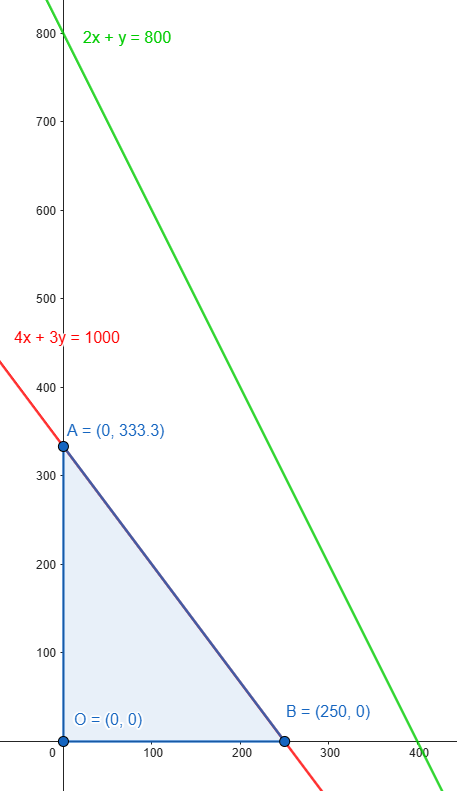
\includegraphics[width=0.37\linewidth]{hw2-1.png}
\end{figure}

\newpage
\section*{Homework 3}
วันสั่ง: 17 สิงหาคม 2568\\
กำหนดส่ง: เสาร์ที่ 23 สิงหาคม 15:00 น.
\subsection*{โจทย์ 1}
\noindent จากโจทย์ ABC Furniture ในเรื่องการกำหนดการเชิงเส้นตามเงื่อนไขที่กำหนดมาให้เราทราบกันมาแล้วว่าตราบใดที่เราสร้างเรากำหนดเงื่อนไขการผลิตโต๊ะ $x$ ตัวและผลิตตู้ $y$ ตัวที่สอดคล้องเงื่อนไขสมการ $4x + 3y = 1000$ ต่างก็จะได้กำไรสูงสุดเช่นกันเสมอ แต่ทั้งนี้สมมติฐานทางธุรกิจของการจะได้กำไรสูงสุดของกำหนดการเชิงเส้นคือต้องสมมติว่าเราจะขายสินค้าที่ผลิตออกมาได้ทั้งหมด ซึ่งอาจจะเป็นไปไม่ได้จริงในสภาวะตลาดที่แตกต่างกัน เพราะบางเวลาโต๊ะก็อาจจะขายได้ดี แต่ในขณะที่บางเวลาตู้ก็อาจจะขายได้ดีกว่า

\textbf{สถานการณ์ทางเลือก:} สำหรับไตรมาสถัดไป ฝ่ายผลิตเสนอ 3 กลยุทธ์ให้ฝ่ายบริหารพิจารณา:

\begin{itemize}
    \item \textbf{กลยุทธ์ A:} ผลิตโต๊ะ 80\% ของการผลิตทั้งหมด
    \item \textbf{กลยุทธ์ B:} ผลิตตู้ 80\% ของการผลิตทั้งหมด
    \item \textbf{กลยุทธ์ C:} ผลิตในอัตราส่วนเท่าๆ กัน
\end{itemize}

\noindent
\textbf{สถานการณ์ตลาด (States of Nature):}  
ฝ่ายการตลาดระบุว่าสถานการณ์ตลาดอาจเป็นไปได้ 3 แบบในไตรมาสหน้า:

\begin{itemize}
    \item \textbf{สถานการณ์ 1 (S1) — โต๊ะบูม:} โต๊ะทำงานขายดีมาก ตู้ขายได้น้อย
    \item \textbf{สถานการณ์ 2 (S2) — ตลาดสมดุล:} สินค้าทั้งสองขายได้ใกล้เคียงกัน
    \item \textbf{สถานการณ์ 3 (S3) — ตู้บูม:} ตู้เอกสารขายดีมาก โต๊ะขายได้น้อย
\end{itemize}

ฝ่ายบริหารต้องการทราบว่า ภายใต้แต่ละกลยุทธ์นั้น ถ้าเกิดสถานการณ์ตลาดแต่ละแบบ จะได้กำไรเท่าไร โดยฝ่ายวิเคราะห์ประเมินกำไร (หน่วย: พันบาท) ดังตาราง:

\begin{center}
\begin{tabular}{|c|c|c|c|}
\hline
\textbf{กลยุทธ์การผลิต} & \textbf{S1: โต๊ะบูม} & \textbf{S2: สมดุล} & \textbf{S3: ตู้บูม} \\
\hline
A (เน้นโต๊ะ) & 422 & 182 & 78 \\
B (เน้นตู้) & 122 & 213 & 378 \\
C (สมดุล) & 284 & 497 & 213 \\
\hline
\end{tabular}
\end{center}

จงตอบคำถามต่อไปนี้
\begin{enumerate}
    \item วิเคราะห์การตัดสินใจภายใต้ความไม่แน่นอนด้วยวิธี maximax
    \item วิเคราะห์การตัดสินใจภายใต้ความไม่แน่นอนด้วยวิธี maximin
    \item ถ้าฝ่ายการตลาดประเมิณมาให้ว่าโอกาสที่จะเกิดตลาดแบบโต๊ะบูม, สมดุล และ ตู้บูมเป็น $25\%, 50\%, 25\%$ ตามลำดับ จงวิเคราะห์การตัดสินใจภายใต้ความเสี่ยงดังกล่าว ด้วยวิธีค่าคาดหวังของกำไร หรือค่าคาดหวังของค่าเสียโอกาสอย่างใดอย่างหนึ่ง
\end{enumerate}

\subsection*{โจทย์ 2}
สถาบันการศึกษาแห่งหนึ่งได้จัดเจ้าหน้าที่เพื่อให้คำปรึกษาวิชาการไว้ 1 คนเพื่อให้คำปรึกษาด้านปัญหาการเรียนแก่นักศึกษา ทว่าได้รับการร้องมาว่าไม่เพียงพอทำให้บางครั้งต้องรอคิวนานจึงกำลังวางแผนจะจ้างเจ้าหน้าที่มาเพิ่มเพราะที่มีอยู่ไม่เพียงพอต่อความต้องการ จึงได้ทำการสำรวจปริมาณการใช้งานในช่วง 1 ชั่วโมง ได้ข้อมูลดังนี้เพื่อจะสุ่มจำลองสถานการณ์โดยใช้เลข 00-99

ข้อมูลการเข้ามารับบริการ\\
\begin{tabular}{|c|c|c|c|c|}
\hline
\textbf{ระยะเวลาที่ห่างกันของการเข้ามา (นาที)} & \textbf{จำนวนนักศึกษา (คน)} & ความน่าจะเป็น & ความน่าจะเป็นสะสม & ช่วงเลขในการสุ่ม \\
\hline 1 & 11 &&&\\
\hline 2 & 29  &&&\\
\hline 3 & 35  &&&\\
\hline 4 & 25  &&&\\
\hline
\end{tabular}

ข้อมูลเวลาในการรับบริการ\\
\begin{tabular}{|c|c|c|c|c|}
\hline
\textbf{เวลาที่ใช้} & \textbf{จำนวนนักศึกษา (คน)} & ความน่าจะเป็น & ความน่าจะเป็นสะสม & ช่วงเลขในการสุ่ม \\
\hline 2 & 15 &&& \\
\hline 3 & 35 &&& \\
\hline 4 & 30 &&& \\
\hline 5 & 20 &&& \\
\hline
\end{tabular}

ได้ทำการจำลองสถานการณ์สำหรับนักศึกษา 10 คน โดยการสุ่มเลขได้ดังตารางด้านล่าง สมมติว่าเริ่มสำรวจตอน 13:00 น.\\
\begin{tabular}{|c|c|c|c|c|c|c|c|c|}
\hline
นิสิต  & เลขสุ่ม   & ระยะห่างเวลา  & เวลาที่ & เวลารอ & เวลาเริ่ม  & เลขสุ่ม &รยะเวลา& เวลาแล้วเสร็จ \\
คนที่ & ระยะห่างเวลา&ระหว่างนักศึกษา& นศ มาถึง &  & ใช้บริการ  & เวลาใช้บริการ &ใช้บริการ& \\
\hline 1 & 53 &&&&&37&& \\
\hline 2 & 74 &&&&&60&& \\
\hline 3 & 05 &&&&&79&& \\
\hline 4 & 71 &&&&&21&& \\
\hline 5 & 06 &&&&&85&& \\
\hline 6 & 49 &&&&&71&& \\
\hline 7 & 11 &&&&&48&& \\
\hline 8 & 13 &&&&&39&& \\
\hline 9 & 62 &&&&&31&& \\
\hline 10 & 69 &&&&&35&& \\
\hline
\end{tabular}

จากตารางการสุ่มที่ได้ จงวิเคราะห์ว่าจำนวนผู้ให้บริการที่มีอยู่เพียงพอหรือไม่

\section*{Homework 4}
วันสั่ง: 24 สิงหาคม 2568\\
กำหนดส่ง: เสาร์ที่ 30 สิงหาคม 15:00 น.

    จากข้อโรงอาหารที่จะได้เมทริกซ์การเปลี่ยนสถานะดังนี้
    \begin{center}
    \begin{tabular}{ll|lll|}
        \cline{3-5}
                                                                     &   & \multicolumn{3}{l|}{เมนูที่ทานเดือนนี้}                   \\ \cline{3-5} 
                                                                     &   & \multicolumn{1}{l|}{A}   & \multicolumn{1}{l|}{B}   & C   \\ \hline
        \multicolumn{1}{|l|}{\multirow{3}{*}{เมนูที่่ทานเดือนถัดไป}} & A & \multicolumn{1}{l|}{0.6} & \multicolumn{1}{l|}{0.6} & 0.2 \\ \cline{2-5} 
        \multicolumn{1}{|l|}{}                                       & B & \multicolumn{1}{l|}{0.3} & \multicolumn{1}{l|}{0.1} & 0.2 \\ \cline{2-5} 
        \multicolumn{1}{|l|}{}                                       & C & \multicolumn{1}{l|}{0.1} & \multicolumn{1}{l|}{0.3} & 0.6 \\ \hline
    \end{tabular}  
    \end{center}
    \begin{enumerate}
        \item จงหาว่าต้องมีอัตราส่วนของคนชอบเมนูอาหารใดเท่าไหร่บ้างถึงจะอยู่ในสภาวะที่ไม่ต้องเปลี่ยนแปลงปริมาณการเก็บวัตถุดิบในเดือนถัดไป (จงหาเวกเตอร์ความน่าจะเป็นที่อยู่ในสถานะคงที่) โดยใช้วิธีการตั้งสมการและแก้ระบบสมการ
        \item ใช้ Excel เพื่อหาเวกเตอร์สถานะคงที่โดยใช้เวกเตอร์ $\begin{pmatrix}
            1 + \text{เลขหลักร้อยของรหัสนักศึกษา}\\
            1 + \text{เลขหลักสิบของรหัสนักศึกษา}\\
            1 + \text{เลขหลักหน่วยของรหัสนักศึกษา}
        \end{pmatrix}$ เป็นเวกเตอร์เริ่มต้น (พิจารณาจำนวนครั้งการคูณกันด้วยตัวเองที่มั่นใจพอว่าเวกเตอร์นิ่งแล้ว) และทำเวกเตอร์สุดท้ายให้อยู่ในรูปเวกเตอร์ความน่าจะเป็น ทำส่งเป็นไฟล์ Excel แนบมาพร้อมกับไฟล์ pdf ของข้อ 1
    \end{enumerate}
    \begin{figure}[h]
        \centering
        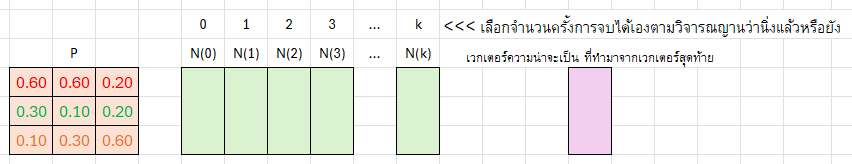
\includegraphics[width=1\linewidth]{Homework4-template.png}
        \caption{ตัวอย่างตาราง Excel (สามารถออกแบบได้ด้วยตัวเอง)}
    \end{figure}
    
\newpage
\section*{Homework 5}
วันสั่ง: 31 สิงหาคม 2568\\
กำหนดส่ง: เสาร์ที่ 6 กันยายน 15:00 น.

\section*{วัตถุประสงค์}
\begin{enumerate}
	\item คำนวณตัวชี้วัดความคลาดเคลื่อน MAE และ RMSE ด้วยมือจากตาราง
	\item เปรียบเทียบความไวต่อ outlier ของ RMSE (ที่ยกกำลังสอง) กับ MAE
	\item ฝึกตีความผลเมื่อมี/ไม่มี outlier ทั้งในชุดฝึกสอนและชุดทดสอบ
\end{enumerate}

\section*{หาตัวแบบ}
\begin{exercise}
	{หาตัวแบบ}{}
	กำหนดชุดข้อมูลมาให้ 6 จุดดังนี้
	\[
	(1,5),\ (2,7),\ (3,9),\ (4,11),\ (5,13),\ \mathbf{(6,50)}
	\]
	โดยที่จุด $(6,50)$ เป็นค่าผิดปกติ (outlier)
	ให้ทำการหาตัวแบบการถดถอยเชิงเส้น 2 อันด้วยการคำนวณด้วยตาราง โดยที่
	\begin{enumerate}
		\item ใช้ข้อมูลครบทั้ง 6 ตัว จะได้ $\hat{y}_{(1)} = \blank{1cm} + \blank{1cm}x$
		\item ใช้แค่ข้อมูล 5 ตัวปกติ จะได้ $\hat{y}_{(2)} = \blank{1cm} + \blank{1cm}x$
	\end{enumerate}
\end{exercise}

\begin{exercise}
	{วัดผลบนชุดข้อมูลที่ใช้สร้างตัวแบบ}{}
	จากตัวแบบที่ได้ในข้อที่ผ่านมา ให้วัดผลด้วย MAE และ RMSE ด้วยชุดข้อมูลที่ใช้
\end{exercise}

\begin{exercise}
	{วัดผลบนชุดข้อมูลใหม่}{}
	จากตัวแบบที่ได้ในข้อที่ผ่านมา ให้วัดผลด้วย MAE และ RMSE ด้วยชุดข้อมูลใหม่ 3 ตัวดังนี้
	\[
	(1.5,6),\ (4.5,12),\ \mathbf{(6.5,55)}
	\]
\end{exercise}

\newpage
\section*{Homework 6}
วันสั่ง: 8 กันยายน 2568\\
กำหนดส่ง: อาทิตย์ที่ 14 กันยายน 21:00 น.

\section*{PART A: ลองคิดกรณีผสมกลยุทธ์ในกรณีที่มีกลยุทธ์แท้}
ตารางค่าผลตอบแทนจากการแข่งขันด้านล่างนี้เป็นตารางของกรณีที่มีกลยุทธ์แท้ กล่าวคือ maximin ของฝ่ายโจมตีมีค่าเท่ากับ minimax การแก้เกมได้ของฝ่ายตั้งรับ
\begin{center}
\begin{tabular}{|c|cc|}
	\hline
	               & \multicolumn{2}{c|}{กลยุทธ์ฝ่ายตรงข้าม}               \\ \hline
	กลยุทธ์ฝ่ายเรา        & \multicolumn{1}{c|}{1}  & \multicolumn{1}{c|}{2}   \\ \hline
	1              & \multicolumn{1}{c|}{4}  & \multicolumn{1}{c|}{3}   \\ \hline
	2              & \multicolumn{1}{c|}{-3} & \multicolumn{1}{c|}{-2}  \\ \hline
\end{tabular}
\end{center}
\textbf{โจทย์:}
\begin{enumerate}
	\item จงหากลยุทธ์แท้ของแต่ละฝ่าย พร้อมทั้งหาค่าของเกม
	\item จงใช้วิธีผสมกลยุทธ์จากฝ่ายเราและวาดแผนภาพแสดงอัตราส่วนของการผสมกลยุทธ์
\end{enumerate}

\section*{PART B: กลยุทธ์ผสม}
ตารางด้านล่างนี้เป็นตารางที่เราได้ดูกันไปในห้องแล้ว และได้ว่าค่าของเกมคือ 36 โดยในห้องเรียนได้พิจารณาการผสมกลยุทธ์ของร้านขาว และการผสมกลยุทธ์แบบสีและแบบผสมของร้านดำไปแล้ว
\begin{center}
	\begin{tabular}{|c|ccc|}
		\hline
		& \multicolumn{3}{c|}{กลยุทธ์ร้านดำ}               \\ \hline
		กลยุทธ์ร้านขาว & \multicolumn{1}{c|}{แบบสี}  & \multicolumn{1}{c|}{แบบขาวดำ}   & \multicolumn{1}{c|}{แบบผสม}\\ \hline
		แบบสี     & \multicolumn{1}{c|}{20}  & \multicolumn{1}{c|}{30}   & \multicolumn{1}{c|}{60}\\ \hline
		แบบขาวดำ   & \multicolumn{1}{c|}{40} & \multicolumn{1}{c|}{45}  & \multicolumn{1}{c|}{30}\\ \hline
	\end{tabular}
\end{center}
ในการบ้านนี้ให้นักศึกษาลองพิจารณาการผสมกลยุทธ์ของแบบสีและแบบขาวดำ (คำเตือน: ต้องพิจารณาแบบ minimax เพราะเป็นตารางผลตอบแทนของร้านขาว)

\newpage
\section*{Homework 7: การบ้านสุดท้าย เตรียมก่อนสอบ}
วันสั่ง: 16 กันยายน 2568\\
กำหนดส่ง: เสาร์ที่ 13 กันยายน 21:00 น.

การบ้านนี้จะเน้นเพื่อเตรียมตัวก่อนสอบ ที่สามารถจดโน๊ตเข้าห้องสอบได้ 1 แผ่นตามคำสั่งหน้าข้อสอบดังนี้
\begin{figure}[h]
	\centering
	
\includegraphics[width=0.7\linewidth]{instruction-final}
\end{figure}

เพราะฉะนั้น ในการบ้านนี้พวกเราจะมาทบทวนสิ่งที่จำเป็นก่อนสอบเพื่อเป็นแนวทางให้นักศึกษาสามารถจดโน๊ตเข้าห้องสอบได้อย่างมีประสิทธิภาพ จงตอบคำถามต่อไปนี้

\section*{การวิเคราะห์มาร์คอฟ}
สูตรในการคำนวณเกี่ยวกับมาร์คอฟมีเพียงสูตรเดียวดังนี้
\begin{equation}
	\vec{N}^{(t+1)} = T\vec{N^{(t)}}
\end{equation}
\begin{enumerate}
	\item เมทริกซ์ความน่าจะเป็นของการเปลี่ยนสถานะ ($T$) จะต้องมีสิ่งที่คำนึงเรื่องการเขียนดังนี้
	\begin{itemize}
		\item การเรียงตัวกันของสถานะในแนวแถวและแนวคอลัมน์ต้องเรียงตัวเหมือนกัน  แต่เพราะเหตุใดเราจึงเขียนการเรียงตัวกันของค่าความน่าจะเป็นในเมทริกซ์การเปลี่ยนสถานะให้ค่าที่มาจากสถานะต้นทางเดียวกันอยู่ในคอลัมน์เดียวกัน และค่าที่มีสถานะปลายทางเดียวกันอยู่ในแถวนอนเดียวกัน
		\item วิธีการหนึ่งที่นักศึกษาจะสามารถตรวจสอบได้ว่านำค่าความน่าจะเป็นของการเปลี่ยนสถานะมาเขียนเรียงกันในเมทริกซ์ได้ถูกต้องหรือไม่คือการดูว่าผลรวมของความน่าจะเป็นในคอลัมน์เดียวกันต้องได้ 1 ในทุก ๆ คอลัมน์ จงอธิบายว่าเพราะเหตุใดถึงทำให้ผลรวมของค่าในคอลัมน์เดียวกันเป็น 1 ในทุก ๆ คอลัมน์
		\item เพราะฉะนั้น ถ้านักศึกษาวาดแผนภาพการเปลี่ยนสถานะได้ดังรูป (ในข้อสอบไม่มีให้วาด) จะได้เมทริกซ์การเปลี่ยนสถานะเป็นอย่างไร
		\begin{center}
			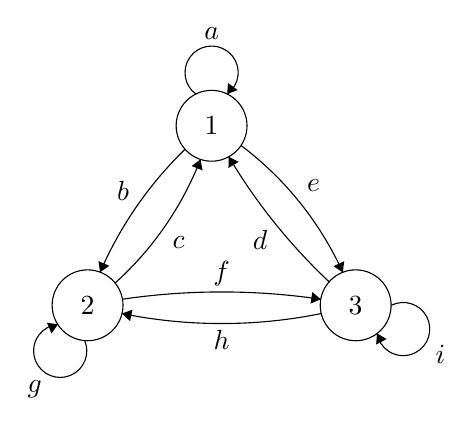
\begin{tikzpicture}[scale=0.15]
				\tikzstyle{every node}+=[inner sep=0pt]
				\draw [black] (41.2,-18.6) circle (3);
				\draw (41.2,-18.6) node {$1$};
				\draw [black] (30.7,-33.8) circle (3);
				\draw (30.7,-33.8) node {$2$};
				\draw [black] (53.4,-33.8) circle (3);
				\draw (53.4,-33.8) node {$3$};
				\draw [black] (40.263,-21.448) arc (-21.32007:-47.95255:27.617);
				\fill [black] (40.26,-21.45) -- (39.51,-22.01) -- (40.44,-22.38);
				\draw (37.86,-28.46) node [right] {$c$};
				\draw [black] (31.764,-30.996) arc (156.57389:134.15349:32.536);
				\fill [black] (31.76,-31) -- (32.54,-30.46) -- (31.62,-30.06);
				\draw (34.25,-24.08) node [left] {$b$};
				\draw [black] (43.691,-20.269) arc (53.08227:24.42099:27.813);
				\fill [black] (52.31,-31.01) -- (52.43,-30.07) -- (51.52,-30.49);
				\draw (49.24,-23.67) node [right] {$e$};
				\draw [black] (51.153,-31.813) arc (-133.25624:-149.24051:48.829);
				\fill [black] (42.65,-21.22) -- (42.63,-22.17) -- (43.49,-21.66);
				\draw (45.97,-28.24) node [left] {$d$};
				\draw [black] (39.877,-15.92) arc (234:-54:2.25);
				\draw (41.2,-11.35) node [above] {$a$};
				\fill [black] (42.52,-15.92) -- (43.4,-15.57) -- (42.59,-14.98);
				\draw [black] (56.388,-33.816) arc (117.43495:-170.56505:2.25);
				\draw (60.13,-37.93) node [right] {$i$};
				\fill [black] (55.21,-36.18) -- (55.13,-37.12) -- (56.02,-36.66);
				\draw [black] (30.455,-36.778) arc (23.03624:-264.96376:2.25);
				\draw (26.23,-40.09) node [below] {$g$};
				\fill [black] (28.19,-35.42) -- (27.26,-35.27) -- (27.65,-36.19);
				\draw [black] (33.655,-33.285) arc (98.39146:81.60854:57.525);
				\fill [black] (50.44,-33.29) -- (49.73,-32.67) -- (49.58,-33.66);
				\draw (42.05,-32.17) node [above] {$f$};
				\draw [black] (50.483,-34.5) arc (-78.53386:-101.46614:42.424);
				\fill [black] (33.62,-34.5) -- (34.3,-35.15) -- (34.5,-34.17);
				\draw (42.05,-35.85) node [below] {$h$};
			\end{tikzpicture}
		\end{center}
	\end{itemize}
	\item เวกเตอร์แสดงอัตราส่วนของแต่ละสถานะ ($\vec{N}$) ซึ่งจะต้องมีลำดับการเรียงตัวของสถานะเหมือนกันกับลำดับของสถานะในเมทริกซ์ $T$
	\begin{itemize}
		\item เราสามารถเขียนแสดงผลได้ 2 แบบคือ (1) เวกเตอร์แสดงจำนวนคนจริง ๆ ในแต่ละสถานะ หรือ (2) เวกเตอร์แสดงความน่าจะเป็นของแต่ละสถานะ แต่ถ้าเรามีเวกเตอร์แสดงจำนวนคนอยู่ก่อน แต่โจทย์ถามเวกเตอร์ความน่าจะเป็น (หรืออัตราส่วน) จะต้องหาอย่างไร
		\item จงคำนวณหาเวกเตอร์แสดงความน่าจะเป็นของแต่ละสถานะจากเวกเตอร์แสดงจำนวนคน $\begin{pmatrix}
			50\\ 80\\ 70
		\end{pmatrix}$
	\end{itemize}
	\item สรุปแล้วลักษณะของปัญหาที่แก้ได้ด้วยการวิเคราะห์มาร์คอฟคือปัญหาแบบใด
\end{enumerate}


\section*{การทำนายและพยากรณ์}
กระบวนการสำคัญของการหาค่าพยากรณ์คือ (1) เตรียมข้อมูล (2) เลือกตัวแบบ (3) คำนวณตัวเบบ และ (4) วัดผลความแม่นยำของการพยากรณ์
\begin{enumerate}
	\item ในการพยากรณ์โดยใช้ตัวแบบอนุกรมเวลา ลำดับของค่าที่จะนำมาพยากรณ์ต้องเป็นอย่างไร
	\item จงระบุสูตรของตัวแบบ และอธิบายวิธีการคำนวณของแต่ละสูตรของการทำตัวแบบอนุกรมเวลา
	\begin{itemize}
		\item Simple moving average ของระยะเวลา $n$ เดือน
		\item Weighted moving average ของระยะเวลา $n$ เดือนแบบกำหนดน้ำหนักด้วยตัวเองเป็น $w_n, w_{n-1}, \dots, w_2, w_1$ ของเดือนย้อนหลัง 1 เดือนจนถึง n เดือนตามลำดับ
		\item Exponential smoothing เหมือนกำหนด $alpha$
	\end{itemize}
	\item ในการวัดผล เราจะใช้วิธีที่เบสิคที่สุดในการวัดผล ซึ่งคือ \textbf{ค่าเฉลี่ยความคลาดเคลื่อนสมบูรณ์} (Mean Absolute Error หรือ Mean Absolute Division) จงระบุสูตรและอธิบายวิธีการคำนวณ 
\end{enumerate}


\section*{ทฤษฎีแถวคอย}
แท้ที่จริงแล้ว ตัวแบบ M/M/1 ก็เป็นกรณีเฉพาะของตัวแบบ M/M/s โดยที่ $s=1$ จงใช้สูตรของ M/M/s เพื่อคำนวณกรณีเฉพาะที่ $s=1$ แล้วดูความแตกต่างระหว่างสูตรของ M/M/1 กับสูตรที่ได้จากการแทน $s=1$ ใน M/M/s


\section*{ทฤษฎีเกม}
ในบททฤษฎีเกม เราสนใจกรณี Zero-sum game กล่าวคือเป็นเกมที่ผู้ชนะได้เท่าไหร่ ผู้แพ้จะเสียเท่านั้น
\begin{enumerate}
	\item ในการคำนวณค่าของเกม สิ่งที่เราสมมติคือผู้เล่นทั้ง 2 ฝ่ายเป็นผู้ที่สามารถเลือกกลยุทธ์การเล่นแบบดีที่สุดได้เสมอ จึงทำให้เข้ารูปแบบการคิดด้วยการใช้ Maximin และการใช้ Minimax คำถามคือเราใช้เกณฑ์อะไรในการตัดสินใจว่าในตารางที่ให้มาผู้เล่นฝ่ายใดต้องใช้ Maximin และผู้เล่นฝ่ายใดต้องใช้ Minimax
	\item ทั้งนี้ ในห้องเรียน อาจารย์ไม่ได้สอนอีกหัวข้อที่อาจารย์ท่านอื่นนำมาออกข้อสอบ ซึ่งคือหัวข้อ ``กลยุทธ์เด่น'' คือการที่ทั้ง 2 ฝ่ายมีกลยุทธ์มากกว่า 2 กลยุทธ์ทั้งคู่ ทำให้เราไม่สามารถใช้วิธีการแบ่งอัตราส่วนอกอเป็น $p, 1-p$ ได้ จึงต้องทำการตัดกลยุทธ์ที่ไม่ดีออกไปก่อน กล่าวคือทำให้เหลือตาราง $2\times n$ หรือ ตาราง $m \times 2$ ให้ได้ก่อน ซึ่งจะใช้วิธีการดูว่ากลยุทธ์ใดที่ให้ผลลัพธ์แย่กว่ากลยุทธ์อื่นในทุก ๆ การเล่นของอีกฝ่าย เราจะตัดกลยุทธ์นั้นทิ้งทันที นักศึกษาสามารถอ่านเพิ่มเติมได้ที่หน้าที่ 282 ในลิงค์ \url{https://blog.bru.ac.th/wp-content/uploads/2024/10/%E0%B9%80%E0%B8%AD%E0%B8%81%E0%B8%AA%E0%B8%B2%E0%B8%A3%E0%B8%9B%E0%B8%A3%E0%B8%B0%E0%B8%81%E0%B8%AD%E0%B8%9A%E0%B8%81%E0%B8%B2%E0%B8%A3%E0%B8%AA%E0%B8%AD%E0%B8%99%E0%B8%A7%E0%B8%B4%E0%B8%8A%E0%B8%B2%E0%B8%81%E0%B8%B2%E0%B8%A3%E0%B8%A7%E0%B8%B4%E0%B9%80%E0%B8%84%E0%B8%A3%E0%B8%B2%E0%B8%B0%E0%B8%AB%E0%B9%8C%E0%B9%80%E0%B8%8A%E0%B8%B4%E0%B8%87%E0%B8%9B%E0%B8%A3%E0%B8%B4%E0%B8%A1%E0%B8%B2%E0%B8%93%E0%B8%97%E0%B8%B2%E0%B8%87%E0%B8%98%E0%B8%B8%E0%B8%A3%E0%B8%81%E0%B8%B4%E0%B8%88-2024.pdf} (ควรจะกดเข้าลิงค์ผ่าน pdf ได้ แต่ถ้ากดไม่ได้อาจารย์จะโพสต์ลิงค์ไว้ในการบ้านอีกที) - และอาจารย์ขอสอนเพิ่มให้ผ่านในวิดีโอ
\end{enumerate}







		\chapter{Quiz}
\newpage
\section*{Quiz 1}
\begin{exercise}{เขียนแบบจำลองและแก้ปัญหาด้วยการวาดรูป}{quiz1}
    บริษัทผลิตอัญมณีแห่งหนึ่งผลิตแหวนและต่างหูจากแร่เงินและแร่ทองคำ โดยที่
    \begin{itemize}
        \item ในการผลิตแหวน จะต้องใช้แร่งทองคำ 3 หน่วย และแร่เงิน 3 หน่วย และจะขายได้กำไร 2 พันบาท
        \item ในการผลิตต่างหู จะต้องใช้แร่งทองคำ 1 หน่วย และแร่เงิน 5 หน่วย และจะขายได้กำไร 1 พันบาท
    \end{itemize}
    ในรอบการผลิตปัจจุบัน บริษัทนี้ได้รับแร่ทองคำมา 18 หน่วย และแร่เงินมา 30 หน่วย โดยที่บริษัทอยากผลิตแหวนและต่างหูให้ได้กำไรมากที่สุด
\end{exercise}

\begin{enumerate}[label=\textbf{ขั้นที่ \arabic*:}, align=left, labelwidth=5em, labelsep=1em, leftmargin=*, itemsep=16pt, topsep=0pt, parsep=0pt, partopsep=0pt]
    \item กำหนดตัวแปร โดยกำหนดให้ $x = \text{จำนวนแหวนที่จะผลิต}$ และ $y = \text{จำนวนต่างหูที่จะผลิต}$
    \item เขียนฟังก์ชันจุดประสงค์ โดยสิ่งที่เป็นเป้าหมายของโจทย์ธุรกิจนี้คืออยาก \blank[1]{1cm} (max ตอบ 0 / min ตอบ 1) ค่ากำไรที่ได้จากการขาย โดยที่
\begin{equation}
    \text{กำไร} = \blank[2]{1.5cm}\ x + \blank[3]{1.5cm}\ y \tag{1}
\end{equation}
    \item เขียนอสมการเงื่อนไข โดยจากโจทย์จะได้ว่ามีเงื่อนไขอยู่ 2 เงื่อนไข คือเงื่อนไขการใช้แร่ทองคำ และเงื่อนไขการใช้แร่เงิน
        \begin{align}
            \text{แร่ทองคำ: }& &\blank[4]{1.5cm}\ x + \blank[5]{1.5cm}\  y &\leq \blank[6]{1.5cm} \tag{2} \\
            \text{แร่เงิน: }& &\blank[7]{1.5cm}\ x + \blank[8]{1.5cm}\  y &\leq \blank[9]{1.5cm}\tag{3} 
        \end{align}
    \item วาดรูปภาพเงื่อนไขจะได้ดังรูปด้านล่างสุด แต่เราจะแบ่งเป็นขั้นตอนการคิดดังนี้
        \begin{enumerate}[label=\textbf{ขั้นที่ 4.\arabic*:}, align=left, itemsep=16pt, topsep=0pt, parsep=0pt, partopsep=0pt]
            \item วาดเส้นเงื่อนไขการใช้แร่ทองคำ (สมการ [2]) โดยการหาจุดตัดแกนทั้ง 2:
                \begin{itemize}[itemsep=16pt]
                    \item หาระยะตัดแกน $x$ โดยการแทน $y = 0$ จะได้สมการ $\blank[4]{1.5cm}\ x = \blank[6]{1.5cm}$
                            ทำให้ได้ว่า $\displaystyle x = \frac{\ \blank[6]{1.5cm}\ }{\ \blank[4]{1.5cm}\ } = \blank[10]{1.5cm} $\\
                            จึงได้ว่าจุดตัดแกน $x$ คือจุด $\left(6,0\right)$
                    \item และในทำนองเดียวกัน จะได้ว่าจุดตัดแกน $y$ คือจุด $\left(0,18\right)$
                \end{itemize}
            \item ในทำนองเดียวกัน เมื่อพิจารณาเงื่อนไขการใช้แร่เงิน (สมการ [3]) \\
                    จะได้ว่าตัดแกน $x$ ที่จุด $\left(10,0\right)$ และตัดแกน $y$ ที่จุด $\left(0,6\right)$
            \item หาจุดตัดระหว่างสมการเส้นขอบของ [2] และสมการเส้นขอบของ [3] จะได้ว่าตัดกันที่จุด $(5,3)$ (+1 คะแนนพิเศษสำหรับคนที่สามารถแก้ระบบสมการเพื่อหาจุดตัดด้วยตัวเองได้: เขียนกระดาษแนบรูปหรือไฟล์ pdf มา)\label{bonus}
        \end{enumerate}
    \item แทนค่าจุดมุมลงในฟังก์ชันจุดประสงค์เพื่อหาค่าแล้วเปรียบเทียบกันว่าจุดใดให้ค่าจุดประสงค์ \blank[11]{1.5cm} (มากสุด ตอบ 0/ น้อยสุด ตอบ 1)\\
    \begin{minipage}{0.35\textwidth}
    \centering
    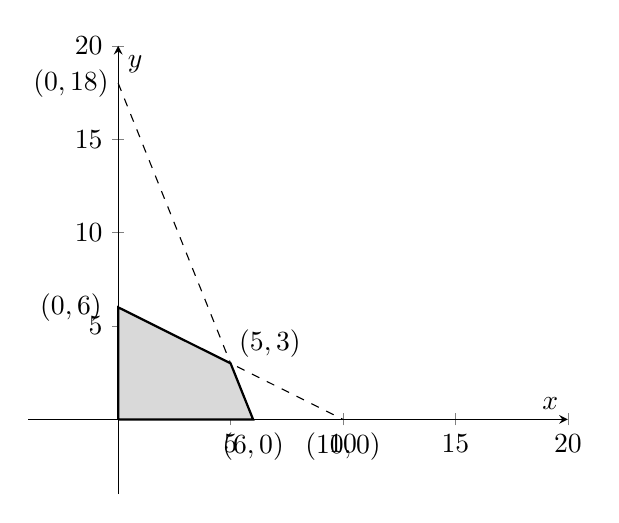
\begin{tikzpicture}[scale=1]
        \begin{axis}[
              axis lines=middle,
              xmin=-4, xmax=20,
              ymin=-4, ymax=20,
              xlabel={$x$}, ylabel={$y$},
            ]
            \addplot[black, dashed, domain=0:6] {18 - 3*x};
            \addplot[black, dashed, domain=0:10] {6 - 3/5*x};
            \addplot[black, thick, fill=gray!30] coordinates {(0,0) (0,6) (5,3) (6,0) (0,0)};
            \node at (axis cs:5,3) [xshift=0.5cm, yshift=0.25cm] {$(5,3)$};
            \node at (axis cs:6,0) [yshift=-0.35cm] {$(6,0)$};
            \node at (axis cs:0,18) [xshift=-0.6cm] {$(0,18)$};
            \node at (axis cs:0,6) [xshift=-0.6cm] {$(0,6)$};
            \node at (axis cs:10,0) [yshift=-0.35cm] {$(10,0)$};
        \end{axis}
    \end{tikzpicture}
\end{minipage}%
\hfill
\begin{minipage}{0.63\textwidth}
    \centering
    \begin{tabular}{c|c}
        $(x,y)$ & กำไร (จากสมการ [1]) \\
        \hline
        $(0,6)$ & \blank[14]{2cm} \\
        \hline
        $(6,0)$ & \blank[15]{2cm} \\
        \hline
        $(5,3)$ & \blank[16]{2cm} \\
        \hline
        $(\blank[12]{1cm},\blank[13]{1cm})$ & \blank[17]{2cm} \\
        \hline
    \end{tabular}
\end{minipage}

    \item สรุปคำตอบ จะได้ค่า \blank[11]{1.5cm} (มากสุด ตอบ 0/ น้อยสุด ตอบ 1) เท่ากับ \blank[18]{1cm} เกิดขึ้นที่จุด $(\blank[19]{1cm},\blank[20]{1cm})$
\end{enumerate}

\subsection*{โบนัสพิเศษ +1 คะแนน}
จงแสดงวิธีการระบบสมการในขั้นที่ \ref{bonus} ว่าได้จุดตัดเป็น $(5,3)$

\newpage
\section*{Quiz 2}
เราจะยังคงใช้โจทย์ปัญหาเดิมกับ quiz 1 อยู่
\begin{exercise}{simplex method}{quiz2}
    บริษัทผลิตอัญมณีแห่งหนึ่งผลิตแหวนและต่างหูจากแร่เงินและแร่ทองคำ โดยที่
    \begin{itemize}
        \item ในการผลิตแหวน จะต้องใช้แร่ทองคำ 3 หน่วย และแร่เงิน 3 หน่วย และจะขายได้กำไร 2 พันบาท
        \item ในการผลิตต่างหู จะต้องใช้แร่ทองคำ 1 หน่วย และแร่เงิน 5 หน่วย และจะขายได้กำไร 1 พันบาท
    \end{itemize}
    ในรอบการผลิตปัจจุบัน บริษัทนี้ได้รับแร่ทองคำมา 18 หน่วย และแร่เงินมา 30 หน่วย โดยที่บริษัทอยากผลิตแหวนและต่างหูให้ได้กำไรมากที่สุด
\end{exercise}

กำหนดให้ $x = \text{จำนวนแหวนที่จะผลิต}$ และ $y = \text{จำนวนต่างหูที่จะผลิต}$ และจาก quiz 1 เราได้โจทย์กำหนดการเชิงเส้นออกมาให้รูป

\begin{multicols}{2}
    \begin{align*}
    \max \quad & 2000x + 1000y\\
    \texttt{subject to} \quad
    & 3x + y \leq 18 \\
    & 3x + 5y \leq 30 \\
    & x \geq 0, \quad y \geq 0 
\end{align*}
และได้บริเวณการตัดสินใจเป็นตามรูปด้านขวา
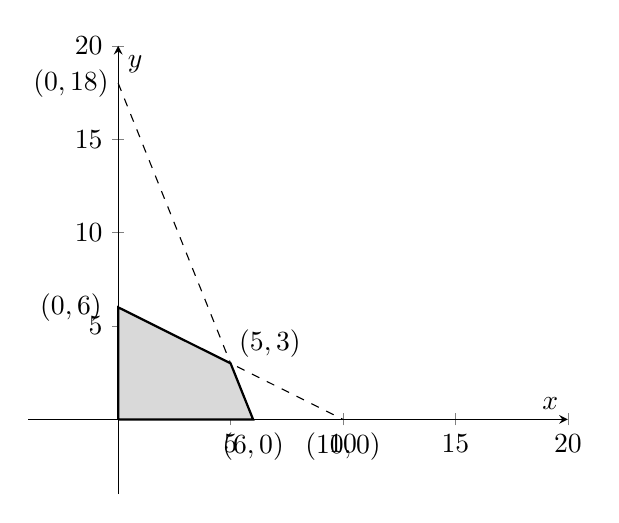
\begin{tikzpicture}[scale=1]
        \begin{axis}[
              axis lines=middle,
              xmin=-4, xmax=20,
              ymin=-4, ymax=20,
              xlabel={$x$}, ylabel={$y$},
            ]
            \addplot[black, dashed, domain=0:6] {18 - 3*x};
            \addplot[black, dashed, domain=0:10] {6 - 3/5*x};
            \addplot[black, thick, fill=gray!30] coordinates {(0,0) (0,6) (5,3) (6,0) (0,0)};
            \node at (axis cs:5,3) [xshift=0.5cm, yshift=0.25cm] {$(5,3)$};
            \node at (axis cs:6,0) [yshift=-0.35cm] {$(6,0)$};
            \node at (axis cs:0,18) [xshift=-0.6cm] {$(0,18)$};
            \node at (axis cs:0,6) [xshift=-0.6cm] {$(0,6)$};
            \node at (axis cs:10,0) [yshift=-0.35cm] {$(10,0)$};
        \end{axis}
    \end{tikzpicture}
\end{multicols}

\begin{multicols}{2}

    และจะแปลงเป็นรูปมาตรฐานได้ดังนี้
    \begin{align*}
        \max \quad & 2000x + 1000y + \blank[]{0.5cm}s_1+ \blank[]{0.5cm}s_2\\
        \texttt{s.t.} \quad
        & 3x + y + s_1 = 18 \\
        & 3x + 5y + s_2 = 30 \\
        & x \geq 0, \quad y \geq 0, \quad s_1 \geq 0, \quad s_2 \geq 0 
    \end{align*}
    และเมื่อนำมาเขียนตารางซิมเพลกซ์ตั้งต้นจะได้ดังนี้
    \begin{center}
        \begin{tabular}{|c|cccc|c|}
            \hline
            \textbf{Pivot} & $x$ & $y$ &  $s_1$ & $s_2$ &  \textbf{RHS} \\
            \hline
            $s_1$ & $3$ & $1$  & $1$ & $0$ & $\blank[]{0.5cm}$ \\
            $s_2$ & $\blank[]{0.5cm}$ & $\blank[]{0.5cm}$  & $\blank[]{0.5cm}$ & $\blank[]{0.5cm}$ & $\blank[]{0.5cm}$ \\
            \hline
            $z$   & $\blank[]{0.5cm}$ & $\blank[]{0.5cm}$  & $\blank[]{0.5cm}$ & $\blank[]{0.5cm}$ & $\blank[]{0.5cm}$ \\
            \hline
        \end{tabular}
    \end{center}
\end{multicols}

ต่อมาเป็นขั้นตอนการเปลี่ยนตัวแปรฐาน โดย
\begin{itemize}
    \item \textbf{ตัวแปรขาเข้า} โดยเลือกใช้ตัวแปรของคอลัมน์ที่มีค่าตัวเลขในแถว $z$ ติดลบมากที่สุด ซึ่งคือตัวแปร \blank[]{1cm}
    \item \textbf{ตัวแปรขาออก} โดยเลือกใช้ตัวแปรที่มีอัตราส่วนระหว่างค่าด้านขวามือ (RHS) กับสัมประสิทธิ์ของตัวแปรขาเข้าค่าบวกที่น้อยที่สุด
    \begin{center}
        \begin{tabular}{|c|cccc|c|c|}
            \hline
            \textbf{Pivot} & $x$ & $y$ &  $s_1$ & $s_2$ &  \textbf{RHS} & อัตราส่วน \\
            \hline
            $s_1$ & $3$ & $1$  & $1$ & $0$ & $\blank[]{0.5cm}$ & $\blank[]{0.5cm} {\Big /} \blank[]{0.5cm} = 6$ \\
            $s_2$ & $\blank[]{0.5cm}$ & $\blank[]{0.5cm}$  & $\blank[]{0.5cm}$ & $\blank[]{0.5cm}$ & $\blank[]{0.5cm}$ & $\blank[]{0.5cm} {\Big /} \blank[]{0.5cm} = 10$ \\
            \hline
            $z$   & $\blank[]{0.5cm}$ & $\blank[]{0.5cm}$  & $\blank[]{0.5cm}$ & $\blank[]{0.5cm}$ & $\blank[]{0.5cm}$ & \\
            \hline
        \end{tabular}
    \end{center}
    ดังนั้น จึงได้ว่าตัวแปรขาออกคือ \blank[]{1cm}
\end{itemize}
และเมื่อทำการดำเนินการตามแถวเพื่อเปลี่ยน pivot ตามขั้นตอนด้านล่างจะได้ตารางซิมเพลกซ์ใหม่ดังนี้
\begin{multicols}{2}
\noindent1. หารแถวของตัวแปรฐานใหม่ด้วยสัมประสิทธิ์ของตัวแปรฐานดังกล่าวในแถวนั้น\\
2. ดำเนินการตามแถวเพื่อให้สัมประสิทธิ์ของตัวแปรฐานในแถวอื่นเป็น 0\\
\begin{tabular}{|c|cccc|c|}
    \hline
    \textbf{Pivot} & $x$ & $y$ &  $s_1$ & $s_2$ &  \textbf{RHS}  \\
    \hline
    $x$ & $1$ & $1/3$  & $1/3$ & $0$ & $6$ \\
    $s_2$ & $0$ & $4$  & $-1$ & $1$ & $12$ \\
    \hline
    $z$   & $0$ & $-1000/3$  & $2000/3$ & $0$ & $12000$ \\
    \hline
\end{tabular}
\end{multicols}

\begin{multicols}{2}
    และถ้าทำซิมเพลกซ์ขั้นถัดไปจะได้ว่าต้องใช้ $y$ เป็นตัวแปรฐานขาเข้า และใช้ $s_2$ เป็นตัวแปรขาออก จะได้ตารางซิมเพลกซ์เป็น

    \begin{tabular}{|c|cccc|c|}
        \hline
        \textbf{Pivot} & $x$ & $y$ &  $s_1$ & $s_2$ &  \textbf{RHS}  \\
        \hline
        $x$ & $1$ & $0$  & $5/12$ & $-1/12$ & $5$ \\
        $y$ & $0$ & $1$  & $-1/4$ & $1/4$ & $3$ \\
        \hline
        $z$   & $0$ & $0$  & $1750/3$ & $250/3$ & $13000$ \\
        \hline
    \end{tabular}
\end{multicols}

ซึ่งไม่มีสมาชิกในแถว $z$ ติดลบแล้วจึงได้ว่ากระบวนการจบสิ้น ซึ่งจะได้ว่าผลเฉลยที่ทำให้ค่ามากสุดคือ $x = 5$ และ $y=3$ (ที่ได้จากคอลัมน์ RHS ในตารางสุดท้าย) และได้ $z = \blank[]{1.5cm}$ เป็นค่ามากสุด

\subsection*{โบนัสพิเศษ +1 คะแนน}
จงใช้ตาราง simplex สุดท้ายแปลงให้เป็นระบบสมการของตัวแปร $x, y, s_1, s_2$ และระบุเหตุผลว่าทำไม $x = 5$ และ $y=3$ โดยอาศัยตัวระบบสมการที่ได้ (คำใบ้: ตัวแปรที่ไม่ใช่ฐานคือตัวแปรที่โดนกำหนดให้ค่าเป็น 0 ดังนั้นต้องระบุให้ได้ก่อนว่าในตารางสุดท้ายใครถูกตั้งบทบาทให้เป็นตัวแปรฐาน)

\newpage
\begin{solution}
    กำหนดให้ $x = \text{จำนวนแหวนที่จะผลิต}$ และ $y = \text{จำนวนต่างหูที่จะผลิต}$ และจาก quiz 1 เราได้โจทย์กำหนดการเชิงเส้นออกมาให้รูป

\begin{multicols}{2}
    \begin{align*}
    \max \quad & 2000x + 1000y\\
    \texttt{subject to} \quad
    & 3x + y \leq 18 \\
    & 3x + 5y \leq 30 \\
    & x \geq 0, \quad y \geq 0 
\end{align*}
และได้บริเวณการตัดสินใจเป็นตามรูปด้านขวา
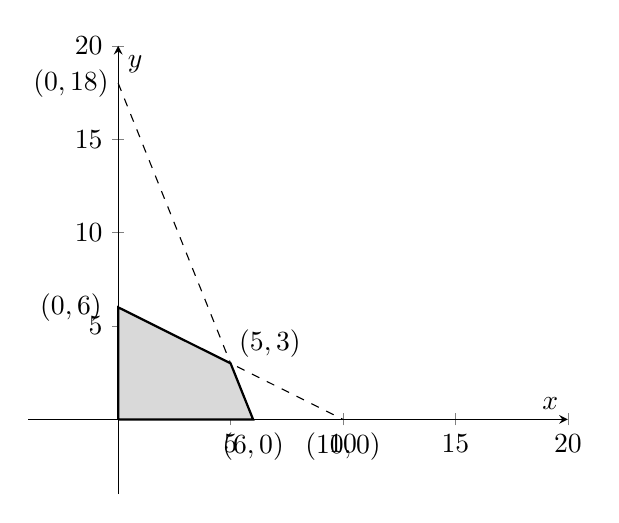
\begin{tikzpicture}[scale=1]
        \begin{axis}[
              axis lines=middle,
              xmin=-4, xmax=20,
              ymin=-4, ymax=20,
              xlabel={$x$}, ylabel={$y$},
            ]
            \addplot[black, dashed, domain=0:6] {18 - 3*x};
            \addplot[black, dashed, domain=0:10] {6 - 3/5*x};
            \addplot[black, thick, fill=gray!30] coordinates {(0,0) (0,6) (5,3) (6,0) (0,0)};
            \node at (axis cs:5,3) [xshift=0.5cm, yshift=0.25cm] {$(5,3)$};
            \node at (axis cs:6,0) [yshift=-0.35cm] {$(6,0)$};
            \node at (axis cs:0,18) [xshift=-0.6cm] {$(0,18)$};
            \node at (axis cs:0,6) [xshift=-0.6cm] {$(0,6)$};
            \node at (axis cs:10,0) [yshift=-0.35cm] {$(10,0)$};
        \end{axis}
    \end{tikzpicture}
\end{multicols}

\begin{multicols}{2}

    และจะแปลงเป็นรูปมาตรฐานได้ดังนี้
    \begin{align*}
        \max \quad & 2000x + 1000y + \blank[0]{0.5cm}s_1+ \blank[0]{0.5cm}s_2\\
        \texttt{s.t.} \quad
        & 3x + y + s_1 = 18 \\
        & 3x + 5y + s_2 = 30 \\
        & x \geq 0, \quad y \geq 0, \quad s_1 \geq 0, \quad s_2 \geq 0 
    \end{align*}
    และเมื่อนำมาเขียนตารางซิมเพลกซ์ตั้งต้นจะได้ดังนี้
    \begin{center}
        \begin{tabular}{|c|cccc|c|}
            \hline
            \textbf{Pivot} & $x$ & $y$ &  $s_1$ & $s_2$ &  \textbf{RHS} \\
            \hline
            $s_1$ & $3$ & $1$  & $1$ & $0$ & $\blank[18]{0.5cm}$ \\
            $s_2$ & $\blank[3]{0.5cm}$ & $\blank[5]{0.5cm}$  & $\blank[0]{0.5cm}$ & $\blank[1]{0.5cm}$ & $\blank[30]{0.5cm}$ \\
            \hline
            $z$   & $\blank[-2000]{1cm}$ & $\blank[-1000]{1cm}$  & $\blank[0]{0.5cm}$ & $\blank[0]{0.5cm}$ & $\blank[0]{0.5cm}$ \\
            \hline
        \end{tabular}
    \end{center}
\end{multicols}

ต่อมาเป็นขั้นตอนการเปลี่ยนตัวแปรฐาน โดย
\begin{itemize}
    \item \textbf{ตัวแปรขาเข้า} โดยเลือกใช้ตัวแปรของคอลัมน์ที่มีค่าตัวเลขในแถว $z$ ติดลบมากที่สุด ซึ่งคือตัวแปร \blank[$x$]{1cm}
    \item \textbf{ตัวแปรขาออก} โดยเลือกใช้ตัวแปรที่มีอัตราส่วนระหว่างค่าด้านขวามือ (RHS) กับสัมประสิทธิ์ของตัวแปรขาเข้าค่าบวกที่น้อยที่สุด
    \begin{center}
        \begin{tabular}{|c|cccc|c|c|}
            \hline
            \textbf{Pivot} & $x$ & $y$ &  $s_1$ & $s_2$ &  \textbf{RHS} & อัตราส่วน \\
            \hline
            $s_1$ & $3$ & $1$  & $1$ & $0$ & $\blank[18]{0.5cm}$ & $\blank[18]{0.5cm} {\Big /} \blank[3]{0.5cm} = 6$ \\
            $s_2$ & $\blank[3]{0.5cm}$ & $\blank[5]{0.5cm}$  & $\blank[0]{0.5cm}$ & $\blank[1]{0.5cm}$ & $\blank[30]{0.5cm}$ & $\blank[30]{0.5cm} {\Big /} \blank[3]{0.5cm} = 10$ \\
            \hline
            $z$   & $\blank[-2000]{1cm}$  & $\blank[-1000]{1cm}$ & $\blank[0]{0.5cm}$ & $\blank[0]{0.5cm}$& $\blank[0]{0.5cm}$  &  \\
            \hline
        \end{tabular}
    \end{center}
    ดังนั้น จึงได้ว่าตัวแปรขาออกคือ \blank[$s_1$]{1cm}
\end{itemize}
และเมื่อทำการดำเนินการตามแถวเพื่อเปลี่ยน pivot ตามขั้นตอนด้านล่างจะได้ตารางซิมเพลกซ์ใหม่ดังนี้
\begin{multicols}{2}
\noindent1. หารแถวของตัวแปรฐานใหม่ด้วยสัมประสิทธิ์ของตัวแปรฐานดังกล่าวในแถวนั้น\\
2. ดำเนินการตามแถวเพื่อให้สัมประสิทธิ์ของตัวแปรฐานในแถวอื่นเป็น 0\\
\begin{tabular}{|c|cccc|c|}
    \hline
    \textbf{Pivot} & $x$ & $y$ &  $s_1$ & $s_2$ &  \textbf{RHS}  \\
    \hline
    $x$ & $1$ & $1/3$  & $1/3$ & $0$ & $6$ \\
    $s_2$ & $0$ & $4$  & $-1$ & $1$ & $12$ \\
    \hline
    $z$   & $0$ & $-1000/3$  & $2000/3$ & $0$ & $12000$ \\
    \hline
\end{tabular}
\end{multicols}

\begin{multicols}{2}
    และถ้าทำซิมเพลกซ์ขั้นถัดไปจะได้ว่าต้องใช้ $y$ เป็นตัวแปรฐานขาเข้า และใช้ $s_2$ เป็นตัวแปรขาออก จะได้ตารางซิมเพลกซ์เป็น

    \begin{tabular}{|c|cccc|c|}
        \hline
        \textbf{Pivot} & $x$ & $y$ &  $s_1$ & $s_2$ &  \textbf{RHS}  \\
        \hline
        $x$ & $1$ & $0$  & $5/12$ & $-1/12$ & $5$ \\
        $y$ & $0$ & $1$  & $-1/4$ & $1/4$ & $3$ \\
        \hline
        $z$   & $0$ & $0$  & $1750/3$ & $250/3$ & $13000$ \\
        \hline
    \end{tabular}
\end{multicols}

ซึ่งไม่มีสมาชิกในแถว $z$ ติดลบแล้วจึงได้ว่ากระบวนการจบสิ้น ซึ่งจะได้ว่าผลเฉลยที่ทำให้ค่ามากสุดคือ $x = 5$ และ $y=3$ (ที่ได้จากคอลัมน์ RHS ในตารางสุดท้าย) และได้ $z = \blank[13000]{1.5cm}$ เป็นค่ามากสุด

\subsection*{โบนัสพิเศษ +1 คะแนน}
จงใช้ตาราง simplex สุดท้ายแปลงให้เป็นระบบสมการของตัวแปร $x, y, s_1, s_2$ และระบุเหตุผลว่าทำไม $x = 5$ และ $y=3$ โดยอาศัยตัวระบบสมการที่ได้ (คำใบ้: ตัวแปรที่ไม่ใช่ฐานคือตัวแปรที่โดนกำหนดให้ค่าเป็น 0 ดังนั้นต้องระบุให้ได้ก่อนว่าในตารางสุดท้ายใครถูกตั้งบทบาทให้เป็นตัวแปรฐาน)

\begin{align*}
    x + \frac{5}{12}s_1 + \frac{-1}{12}s_2 &= 5\\
    y + \frac{-1}{4}s_1 + \frac{1}{4}s_2 &= 3\\
    z + \frac{1750}{3}s_1 + \frac{250}{3}s_2 &= 13000
\end{align*}

โดยที่มี $x,y$ เป็นตัวแแปรฐาน ดังนั้น $s_1,s_2$ ที่ไม่ใช่ตัวแปรฐานจึงมีค่าเท่ากับ $0$ จึงได้ว่า
\begin{align*}
    x + \frac{5}{12}(0) + \frac{-1}{12}(0) &= 5 &\Rightarrow x &= 5\\
    y + \frac{-1}{4}(0) + \frac{1}{4}(0) &= 3 &\Rightarrow y &= 3\\
    z + \frac{1750}{3}(0) + \frac{250}{3}(0) &= 13000&\Rightarrow z &= 13000
\end{align*}
\end{solution}

\newpage
\section*{Quiz 3}
ในการสอบย่อยครั้งนี้ เราจะมาฝึกคูณเมทริกซ์กับเทริกซ์โดยอาศัยรูปภาพของการเปลี่ยนสถานะแบบมาร์คอฟกัน
\begin{exercise}{หาผลกำลังสองของเมทริกซ์ความน่าจะเปลี่ยนของการเปลี่ยนสถานะ}{quiz3}
	จงหาผลคูณของเมทริกซ์ได้ผลลัพธ์ดังนี้ (โจทย์ให้ผลลัพธ์การคูณมาแล้ว ดังนั้นไม่ต้องนั่งคูณด้วยตัวเอง แต่เราจะลองใช้ความรู้ Markov ช่วยหาผลคูณ และในข้อนี้เราจะไม่ได้หาผลคูณของทั้ง 9 ตัว เราจะยกตัวอย่างการหาผลคูณของแค่ 3 ตัวเท่านั้น)
	$$
	\begin{bmatrix}
		0.6 & 0.6 & 0.2 \\
		0.3 & 0.1 & 0.2 \\
		0.1 & 0.3 & 0.6 \\
	\end{bmatrix} \times
	\begin{bmatrix}
		0.6 & 0.6 & 0.2 \\
		0.3 & 0.1 & 0.2 \\
		0.1 & 0.3 & 0.6 \\
	\end{bmatrix}
	=
	\begin{bmatrix}
		0.56 & 0.48 & 0.36 \\
		0.23 & 0.25 & 0.20 \\
		0.21 & 0.27 & 0.44 \\
	\end{bmatrix}
	$$
\end{exercise}

เริ่มจากเขียนแผนภาพการเปลี่ยนสถานะกันก่อน โดยโจทย์คือให้\underline{\textbf{เขียนค่าความน่าจะเป็นลงไปบนเส้นการเปลี่ยนสถานะ}}
\begin{center}
	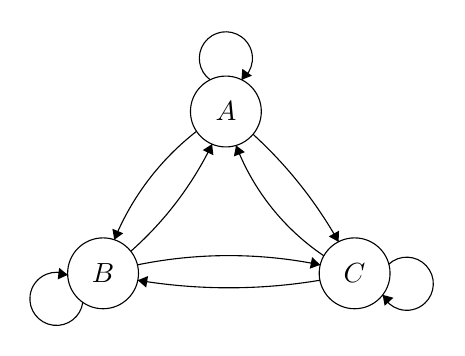
\begin{tikzpicture}[scale=0.15]
		\tikzstyle{every node}+=[inner sep=0pt]
		\draw [black] (23.7,-25.4) circle (3);
		\draw (23.7,-25.4) node {$A$};
		\draw [black] (13.3,-39.1) circle (3);
		\draw (13.3,-39.1) node {$B$};
		\draw [black] (34.6,-39.1) circle (3);
		\draw (34.6,-39.1) node {$C$};
		\draw [black] (14.249,-36.256) arc (157.70826:127.88572:22.39);
		\fill [black] (14.25,-36.26) -- (15.01,-35.71) -- (14.09,-35.33);
		\draw [black] (22.535,-28.163) arc (-25.83943:-48.56659:28.903);
		\fill [black] (22.53,-28.16) -- (21.74,-28.67) -- (22.64,-29.1);
		\draw [black] (16.213,-38.384) arc (101.57892:78.42108:38.549);
		\fill [black] (31.69,-38.38) -- (31,-37.73) -- (30.8,-38.71);
		\draw [black] (31.659,-39.688) arc (-80.52759:-99.47241:46.841);
		\fill [black] (16.24,-39.69) -- (16.95,-40.31) -- (17.11,-39.33);
		\draw [black] (25.997,-27.328) arc (47.64144:29.37151:36.624);
		\fill [black] (33.24,-36.43) -- (33.28,-35.49) -- (32.41,-35.98);
		\draw [black] (31.995,-37.618) arc (-123.95959:-159.02746:19.823);
		\fill [black] (24.56,-28.27) -- (24.38,-29.2) -- (25.31,-28.84);
		\draw [black] (22.377,-22.72) arc (234:-54:2.25);
		\fill [black] (25.02,-22.72) -- (25.9,-22.37) -- (25.09,-21.78);
		\draw [black] (37.487,-38.329) arc (132.69007:-155.30993:2.25);
		\fill [black] (36.97,-40.92) -- (37.14,-41.85) -- (37.88,-41.17);
		\draw [black] (11.585,-41.547) arc (-7.29476:-295.29476:2.25);
		\fill [black] (10.31,-39.23) -- (9.58,-38.63) -- (9.46,-39.62);
	\end{tikzpicture}
\end{center}


จากที่เรียนมาในห้อง เราทราบกันอยู่แล้วว่าความหมายของการนำเมทริกซ์การเปลี่ยนสถานะ 1 ขั้นมาคูณกัน จะได้ผลออกมาเป็นเมทริกซ์การเปลี่ยนสถานะข้าม 2 ขั้น (เช่นเปลี่ยนจากขั้นที่ 1 ไปขั้นที่ 3)
ดังนั้น ถ้าเราอยากหาผลคูณของเมทริกซ์การเปลี่ยนสถานะ สิ่งที่ต้องทำคือหาความน่าจะเป็นในการเดินข้าม 2 ขั้นทุกรูปแบบที่เป็นไปได้

\subsubsection*{การเปลี่ยนสถานะจาก A ในขั้นที่ 1 ไป A ในขั้นที่ 3}
วาดแผนภาพด้านล่าง โจทย์คือ \underline{\textbf{จงเขียนค่าความน่าจะเป็นของการย้ายสถานะของแต่ละเส้น (มี 6 เส้น)}}
\begin{center}
	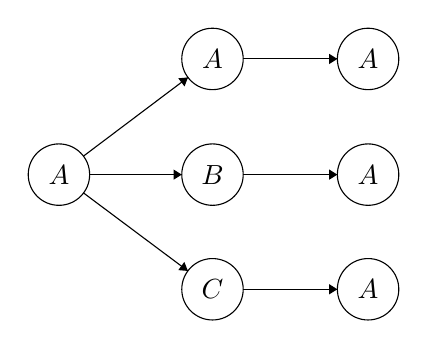
\begin{tikzpicture}[scale=0.13]
		\tikzstyle{every node}+=[inner sep=0pt]
		\draw [black] (11,-31.3) circle (3);
		\draw (11,-31.3) node {$A$};
		\draw [black] (26,-31.3) circle (3);
		\draw (26,-31.3) node {$B$};
		\draw [black] (26,-42.5) circle (3);
		\draw (26,-42.5) node {$C$};
		\draw [black] (26,-20) circle (3);
		\draw (26,-20) node {$A$};
		\draw [black] (41.2,-20) circle (3);
		\draw (41.2,-20) node {$A$};
		\draw [black] (41.2,-31.3) circle (3);
		\draw (41.2,-31.3) node {$A$};
		\draw [black] (41.2,-42.5) circle (3);
		\draw (41.2,-42.5) node {$A$};
		\draw [black] (13.4,-29.49) -- (23.6,-21.81);
		\fill [black] (23.6,-21.81) -- (22.66,-21.89) -- (23.27,-22.69);
		\draw [black] (14,-31.3) -- (23,-31.3);
		\fill [black] (23,-31.3) -- (22.2,-30.8) -- (22.2,-31.8);
		\draw [black] (13.4,-33.09) -- (23.6,-40.71);
		\fill [black] (23.6,-40.71) -- (23.25,-39.83) -- (22.66,-40.63);
		\draw [black] (29,-20) -- (38.2,-20);
		\fill [black] (38.2,-20) -- (37.4,-19.5) -- (37.4,-20.5);
		\draw [black] (29,-31.3) -- (38.2,-31.3);
		\fill [black] (38.2,-31.3) -- (37.4,-30.8) -- (37.4,-31.8);
		\draw [black] (29,-42.5) -- (38.2,-42.5);
		\fill [black] (38.2,-42.5) -- (37.4,-42) -- (37.4,-43);
	\end{tikzpicture}
\end{center}

ด้วยความรู้ในเรื่องความน่าจะเป็น เราจะได้ว่าความน่าจะเป็นรวมของการย้ายสถานะจาก A ข้ามไป A ใน 2 ขั้นถัดไปหาได้จากกฏการคูณและการบวกจากแผนภาพต้นไม้ดังกล่าว โดยที่
\begin{itemize}
	\item เส้นต่อกัน ให้นำค่าความน่าจะเป็นของเส้นมาคูณกัน
	\item หลังจากคิดผลคูณค่าความน่าจะเป็นของแต่ละกิ่งเรียบร้อยแล้ว ให้นำมาบวกกัน
\end{itemize}
เพราะฉะนั้น เราจะได้ว่าความน่าจะเป็นของการเปลี่ยนสถานะจาก A ข้ามไป A ใน 2 ขั้นถัดไปมีค่าเท่ากับ
$$
P(A\rightarrow_2A) = \left(\blank{1cm}\times\blank{1cm}\right) + \left(\blank{1cm}\times\blank{1cm}\right) + \left(\blank{1cm}\times\blank{1cm}\right) = 0.56
$$
ซึ่งมีผลลัพธ์เท่ากับสมาชิกในแถวที่ 1 หลักที่ 1 ที่แทนความน่าจะเป็นของการเปลี่ยนจาก A ไป A ในเมทริกซ์ผลลัพธ์
\subsubsection*{การเปลี่ยนสถานะจาก A ในขั้นที่ 1 ไป B ในขั้นที่ 3}
วาดแผนภาพด้านล่าง โจทย์คือ \underline{\textbf{จงเขียนค่าความน่าจะเป็นของการย้ายสถานะของแต่ละเส้น (มี 6 เส้น)}}
\begin{center}
	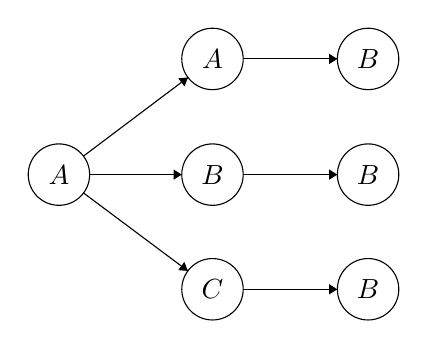
\begin{tikzpicture}[scale=0.13]
		\tikzstyle{every node}+=[inner sep=0pt]
		\draw [black] (11,-31.3) circle (3);
		\draw (11,-31.3) node {$A$};
		\draw [black] (26,-31.3) circle (3);
		\draw (26,-31.3) node {$B$};
		\draw [black] (26,-42.5) circle (3);
		\draw (26,-42.5) node {$C$};
		\draw [black] (26,-20) circle (3);
		\draw (26,-20) node {$A$};
		\draw [black] (41.2,-20) circle (3);
		\draw (41.2,-20) node {$B$};
		\draw [black] (41.2,-31.3) circle (3);
		\draw (41.2,-31.3) node {$B$};
		\draw [black] (41.2,-42.5) circle (3);
		\draw (41.2,-42.5) node {$B$};
		\draw [black] (13.4,-29.49) -- (23.6,-21.81);
		\fill [black] (23.6,-21.81) -- (22.66,-21.89) -- (23.27,-22.69);
		\draw [black] (14,-31.3) -- (23,-31.3);
		\fill [black] (23,-31.3) -- (22.2,-30.8) -- (22.2,-31.8);
		\draw [black] (13.4,-33.09) -- (23.6,-40.71);
		\fill [black] (23.6,-40.71) -- (23.25,-39.83) -- (22.66,-40.63);
		\draw [black] (29,-20) -- (38.2,-20);
		\fill [black] (38.2,-20) -- (37.4,-19.5) -- (37.4,-20.5);
		\draw [black] (29,-31.3) -- (38.2,-31.3);
		\fill [black] (38.2,-31.3) -- (37.4,-30.8) -- (37.4,-31.8);
		\draw [black] (29,-42.5) -- (38.2,-42.5);
		\fill [black] (38.2,-42.5) -- (37.4,-42) -- (37.4,-43);
	\end{tikzpicture}
\end{center}

เพราะฉะนั้น เราจะได้ว่าความน่าจะเป็นของการเปลี่ยนสถานะจาก A ข้ามไป B ใน 2 ขั้นถัดไปมีค่าเท่ากับ
$$
P(A\rightarrow_2B) = \left(\blank{1cm}\times\blank{1cm}\right) + \left(\blank{1cm}\times\blank{1cm}\right) + \left(\blank{1cm}\times\blank{1cm}\right) = \blank{1cm}
$$
\subsection*{โบนัสพิเศษ +1 คะแนน (แบบไม่หาร)}
จาก 2 ตัวอย่างที่ผ่านมา น่าจะพอสังเกตลักษณะการนำตัวเลขในเมทริกซ์มาคูณไขว้กันได้ จงอธิบายวิธีการคิดการคูณเมทริกซ์กับเมทริกซ์จากข้อสังเกตที่ได้ พร้อมทั้งแสดงวิธีคำนวณการคูณเพื่อหาสมาชิกอีก 7 ตัวที่เหลือ 
		% \chapter{Handnote}
\newpage
\includepdf[pages=-]{Quantitative_Analysis_250803.pdf}
\includepdf[pages=-]{Quantitative_Analysis_250810.pdf}
\includepdf[pages=-]{Quantitative_Analysis_250817.pdf}
\includepdf[pages=-]{Quantitative_Analysis_250824.pdf}
\includepdf[pages=-]{Quantitative_Analysis_250831.pdf}
\includepdf[pages=-]{Quantitative_Analysis_250907.pdf}
	\end{appendices}
	
	% !TEX root = ../BookTemplate.tex
%%%%%%%%%%%%%%%%%%%%%%%%%%%%%%%%%%%%%%%%%%%%%%%%%%%%%%%%%%%%%%%%%%%%%%%%%%%%%%%%%%
\backmatter

%%%%%%%%%                       (BIBLIOGRAPHY PAGE FORMAT)
\fancypagestyle{fancyBibliography}{
	\renewcommand{\headrulewidth}{0.25pt}
	\renewcommand{\footrulewidth}{0.25pt}
	\fancyfoot[LE,RO]{}
	\fancyhead[LO,RE]{\bf\small \BibliographyName}}

%%%%%%%%%%                      (ANALYTIC INDEX PAGE FORMAT)
\fancypagestyle{fancyIndex}{
	\renewcommand{\headrulewidth}{0.25pt}
	\renewcommand{\footrulewidth}{0.25pt}
	\fancyhead[L,R]{}
	\fancyfoot[L,R]{}
	\fancyfoot[C]{\small\thepage}
	\fancyfoot[LE,RO]{}
	\fancyhead[LO,RE]{\bf\small \AnalyticIndexName}}

%%%%%%%%%%%%%%%%%%%%%%%%%%%%    (BIBLIOGRAPHY)
\pagestyle{fancyBibliography}
\renewcommand{\bibname}{}

\titleformat{\chapter}[display]{\bfseries\Large}	{\filleft\MakeUppercase{\chaptertitlename} \HUGE\thechapter}{.4ex}{\vspace{1ex}\filleft}[\vspace{3.5ex}]
\titlespacing*{\chapter}{0pt}{0.1\baselineskip}{0.5\baselineskip}

{
    \let\cleardoublepage\relax
    \begin{minipage}[r]{.95\textwidth}\raggedleft
    \vspace{3cm}
    \HUGE\bfseries\BibliographyName
	\vspace{0cm}
    \end{minipage}
	\addcontentsline{toc}{part}{\BibliographyName}
    
	\nocite{*}
	\bibliographystyle{amsalpha}
	\bibliography{Structure/Bibliography}
}

\cleardoublepage

%%%%%%%%%%%%%%%%%%%%%%%%%%%%    (ANALYTIC INDEX)
 \pagestyle{fancyIndex}
 	\renewcommand{\indexname}{}
	\let\cleardoublepage\relax
    \titleformat{\chapter}[hang]{}{}{0em}{}[]
 	
    \chapter*{}
	\titleformat{\chapter}
		[hang]
		{\Huge}
		{}
		{0em}
		{}
		[\Large {\begin{tikzpicture} [remember picture, overlay]
		\pgftext[right,x=14.75cm,y=0.2cm]{\HUGE\bfseries 
			\AnalyticIndexName}
		\end{tikzpicture}}]
	\titlespacing*{\chapter}{0pt}{0\baselineskip}{5\baselineskip}

    \addcontentsline{toc}{part}{\AnalyticIndexName}	
	%\vspace{-2cm}
	\printindex    %%%%%%%%%%%%%%%%%%          (DO NOT EDIT)
	
\end{document}
